\documentclass[twoside]{book}

% Packages required by doxygen
\usepackage{fixltx2e}
\usepackage{calc}
\usepackage{doxygen}
\usepackage[export]{adjustbox} % also loads graphicx
\usepackage{graphicx}
\usepackage[utf8]{inputenc}
\usepackage{makeidx}
\usepackage{multicol}
\usepackage{multirow}
\PassOptionsToPackage{warn}{textcomp}
\usepackage{textcomp}
\usepackage[nointegrals]{wasysym}
\usepackage[table]{xcolor}

% Font selection
\usepackage[T1]{fontenc}
\usepackage[scaled=.90]{helvet}
\usepackage{courier}
\usepackage{amssymb}
\usepackage{sectsty}
\renewcommand{\familydefault}{\sfdefault}
\allsectionsfont{%
  \fontseries{bc}\selectfont%
  \color{darkgray}%
}
\renewcommand{\DoxyLabelFont}{%
  \fontseries{bc}\selectfont%
  \color{darkgray}%
}
\newcommand{\+}{\discretionary{\mbox{\scriptsize$\hookleftarrow$}}{}{}}

% Page & text layout
\usepackage{geometry}
\geometry{%
  a4paper,%
  top=2.5cm,%
  bottom=2.5cm,%
  left=2.5cm,%
  right=2.5cm%
}
\tolerance=750
\hfuzz=15pt
\hbadness=750
\setlength{\emergencystretch}{15pt}
\setlength{\parindent}{0cm}
\setlength{\parskip}{3ex plus 2ex minus 2ex}
\makeatletter
\renewcommand{\paragraph}{%
  \@startsection{paragraph}{4}{0ex}{-1.0ex}{1.0ex}{%
    \normalfont\normalsize\bfseries\SS@parafont%
  }%
}
\renewcommand{\subparagraph}{%
  \@startsection{subparagraph}{5}{0ex}{-1.0ex}{1.0ex}{%
    \normalfont\normalsize\bfseries\SS@subparafont%
  }%
}
\makeatother

% Headers & footers
\usepackage{fancyhdr}
\pagestyle{fancyplain}
\fancyhead[LE]{\fancyplain{}{\bfseries\thepage}}
\fancyhead[CE]{\fancyplain{}{}}
\fancyhead[RE]{\fancyplain{}{\bfseries\leftmark}}
\fancyhead[LO]{\fancyplain{}{\bfseries\rightmark}}
\fancyhead[CO]{\fancyplain{}{}}
\fancyhead[RO]{\fancyplain{}{\bfseries\thepage}}
\fancyfoot[LE]{\fancyplain{}{}}
\fancyfoot[CE]{\fancyplain{}{}}
\fancyfoot[RE]{\fancyplain{}{\bfseries\scriptsize Generated by Doxygen }}
\fancyfoot[LO]{\fancyplain{}{\bfseries\scriptsize Generated by Doxygen }}
\fancyfoot[CO]{\fancyplain{}{}}
\fancyfoot[RO]{\fancyplain{}{}}
\renewcommand{\footrulewidth}{0.4pt}
\renewcommand{\chaptermark}[1]{%
  \markboth{#1}{}%
}
\renewcommand{\sectionmark}[1]{%
  \markright{\thesection\ #1}%
}

% Indices & bibliography
\usepackage{natbib}
\usepackage[titles]{tocloft}
\setcounter{tocdepth}{3}
\setcounter{secnumdepth}{5}
\makeindex

% Hyperlinks (required, but should be loaded last)
\usepackage{ifpdf}
\ifpdf
  \usepackage[pdftex,pagebackref=true]{hyperref}
\else
  \usepackage[ps2pdf,pagebackref=true]{hyperref}
\fi
\hypersetup{%
  colorlinks=true,%
  linkcolor=blue,%
  citecolor=blue,%
  unicode%
}

% Custom commands
\newcommand{\clearemptydoublepage}{%
  \newpage{\pagestyle{empty}\cleardoublepage}%
}

\usepackage{caption}
\captionsetup{labelsep=space,justification=centering,font={bf},singlelinecheck=off,skip=4pt,position=top}

%===== C O N T E N T S =====

\begin{document}

% Titlepage & ToC
\hypersetup{pageanchor=false,
             bookmarksnumbered=true,
             pdfencoding=unicode
            }
\pagenumbering{alph}
\begin{titlepage}
\vspace*{7cm}
\begin{center}%
{\Large Raft\+Lib \\[1ex]\large 0.\+9a }\\
\vspace*{1cm}
{\large Generated by Doxygen 1.8.12}\\
\end{center}
\end{titlepage}
\clearemptydoublepage
\pagenumbering{roman}
\tableofcontents
\clearemptydoublepage
\pagenumbering{arabic}
\hypersetup{pageanchor=true}

%--- Begin generated contents ---
\chapter{Command Args}
\label{md_git-dep_cmdargs__r_e_a_d_m_e}
\hypertarget{md_git-dep_cmdargs__r_e_a_d_m_e}{}
Super simple command arguments parser for C++. Yeah, there are quite a few already in existence, but I made this for a particular purpose, ended up using it quite a bit so it\textquotesingle{}s worth it at this point to put it up on Git\+Hub so I can download it from multiple points.

\#\+Build Status \href{https://travis-ci.org/RaftLib/cmdargs}{\tt }

\#\+Notes There are a few bugs here and there, notably there are a few instances where there are null arguments that I\textquotesingle{}d like to pass but it\textquotesingle{}s easy enough to get around by adding an explicit boolean.

\#\+Compiling is super simple\+:


\begin{DoxyCode}
mkdir build
cd build
cmake ../cmdargs
make
sudo make install
\end{DoxyCode}


which installs all the library code and header files in the appropriate /usr/local prefix. I\textquotesingle{}ve used on both OS X and Linux, I\textquotesingle{}ll check to see if it works on Windows when I get a chance.

\#\#\+Simple Example 
\begin{DoxyCode}
\hyperlink{class_cmd_args}{CmdArgs}  cmd( argv[ 0 ],
              std::cout,
              std::cerr );

\textcolor{keywordtype}{bool} help( \textcolor{keyword}{false} );

cmd.addOption( \textcolor{keyword}{new} Option< bool >( help,
                                    \textcolor{stringliteral}{"-h"},
                                    \textcolor{stringliteral}{"Print this message"},
                                    \textcolor{keyword}{false},
                                    \textcolor{keyword}{true} ) );
\textcolor{keywordtype}{bool} printHeader( \textcolor{keyword}{false} );
cmd.addOption( \textcolor{keyword}{new} Option< bool >( printHeader,
                                    \textcolor{stringliteral}{"-header"},
                                    \textcolor{stringliteral}{"Print the header and exit"} ) );


cmd.addOption( \textcolor{keyword}{new} Option< std::string >( filename,
                                          \textcolor{stringliteral}{"-f"},
                                          \textcolor{stringliteral}{"Set the output file name"},
                                          \textcolor{keyword}{true} \textcolor{comment}{/** make this arg mandatory **/} ) );

cmd.addOption( \textcolor{keyword}{new} Option< int64\_t >( length, 
                                      \textcolor{stringliteral}{"-l"},
                                      \textcolor{stringliteral}{"Length of run"} ) );
cmd.addOption( \textcolor{keyword}{new} Option< int64\_t >( buff\_size,
                                      \textcolor{stringliteral}{"-b"},
                                      \textcolor{stringliteral}{"Buffer size"} ) );

cmd.addOption( \textcolor{keyword}{new} Option< int64\_t >( repeat,
                                      \textcolor{stringliteral}{"-r"},
                                      \textcolor{stringliteral}{"Number of times to repeat simulation"} ) );

cmd.processArgs( argc, argv );
\textcolor{comment}{}
\textcolor{comment}{/** give object command line **/}
cmd.processArgs( argc, argv );
\textcolor{comment}{}
\textcolor{comment}{/** handle the user needing help **/}
\textcolor{keywordflow}{if}( help )
\{
   cmd.printArgs();
   exit( EXIT\_SUCCESS );
\}\textcolor{comment}{}
\textcolor{comment}{/** }
\textcolor{comment}{ * to check and see if all mandatory args are set, add this code}
\textcolor{comment}{ * which will print all mandatory args that are missing.}
\textcolor{comment}{ */}
\textcolor{keywordflow}{if}( cmd.allMandatorySet() )
\{ 
   \textcolor{comment}{//exit since well, mandatory args missing}
   exit( EXIT\_FAILURE );
\}
\end{DoxyCode}


Enjoy, feel free to update, copy or fix as you feel the need to. 
\chapter{R\+E\+A\+D\+ME}
\label{md_git-dep_shm__r_e_a_d_m_e}
\hypertarget{md_git-dep_shm__r_e_a_d_m_e}{}
\#\+Description Easy S\+HM library for C++, still a work in progress but it\textquotesingle{}s a easier way to code up an anonymous S\+HM mapping, protect the last page and generate a key to access it....I\textquotesingle{}ve used similar code quite a bit and was tired of re-\/coding it. If I find time I\textquotesingle{}ll make it a bit more advanced, like adding a monitor process to cleanup if for some reason the code crashes (you know, things happen right?). I\textquotesingle{}ve tested the code on OS X and Linux, but as usual your mileage may vary greatly.

\#\+Build Status \href{https://travis-ci.org/RaftLib/shm}{\tt }

\#\+Important Notes So I\textquotesingle{}ve checked the functions found in the testsuite. I\textquotesingle{}ve used the code quite a bit in various forms so it should work rather well...however if you find bugs please submit a pull request and I\textquotesingle{}ll get it fixed A\+S\+AP.

\#\+Compilation Notes To build this library on OS X you\textquotesingle{}ll need to run\+: glibtoolize aclocal autoconf automake --add-\/missing make make check sudo make intall

The only changes for linux will be libtoolize for call to libtool instead of glibtoolize...on OS X the binary might be named differently depending on how you\textquotesingle{}ve installed it so your mileage may vary. If you\textquotesingle{}re advanced enough to install libtool on OS X you should be able to figure this out.

\#\+Usage To use this library, simply\+: \#include $<$shm$>$

When compiling your code that uses it, link with -\/lshm. On Linux you\textquotesingle{}ll have to compile with the -\/lrt, -\/lpthread and -\/lnuma in order to fully utilize all the features. In the future I might add a flag to compile without the N\+U\+MA features so that you can use the library without having to install libnuma.

\#\+Parting Thoughts Hopefully everything will work well....there are fairly good comments if you\textquotesingle{}re interested in the S\+HM header file under /include. 
\chapter{R\+E\+A\+D\+ME}
\label{md__r_e_a_d_m_e}
\hypertarget{md__r_e_a_d_m_e}{}
============= \subsubsection*{Pre-\/requisites}

\paragraph*{O\+S X}

Compiler\+: Clang, G\+N\+U G\+C\+C 4.\+8+, or Intel icc Libraries\+:
\begin{DoxyItemize}
\item Only for random number generators \href{http://goo.gl/gchdSw}{\tt G\+N\+U G\+S\+L}
\item Only for partitioning, basic download doesn\textquotesingle{}t need\+: \href{http://goo.gl/tI1NGf}{\tt Scotch} \paragraph*{Linux}
\end{DoxyItemize}

Compiler\+: c++11 capable Libraries\+:
\begin{DoxyItemize}
\item Only for random number generators \href{http://goo.gl/gchdSw}{\tt G\+N\+U G\+S\+L}
\item Only for partitioning, basic download doesn\textquotesingle{}t need\+: \href{http://goo.gl/tI1NGf}{\tt Scotch}
\end{DoxyItemize}

\subsubsection*{Install}

Once the optional pre-\/requisite libraries are installed, make a build directory (for the instructions below, we\textquotesingle{}ll write \mbox{[}build\mbox{]}). 
\begin{DoxyCode}
1 cd [build]
2 cmake ../[build]
3 make
4 sudo make install
\end{DoxyCode}
 N\+O\+T\+E\+: The default prefix in the makefile is 
\begin{DoxyCode}
1 PREFIX ?= /usr/local
\end{DoxyCode}
 The old Makefile had an uninstall script, I need to add an object to the cmake file so that we can have similar functionality.

N\+O\+T\+E\+: still working on cmake/re-\/arrangeing. C\+Make basically works tested on O\+S X and Linux. I\textquotesingle{}ll have more time for re-\/arrangements and the sub-\/modules sometime this week (19 Nov. 2015) 
\chapter{Notes}
\label{md_testsuite__t_o_d_o}
\hypertarget{md_testsuite__t_o_d_o}{}
The following test cases build and work on OS X Yosemite and Linux using Intel I\+CC and G\+NU G\+CC 4.\+9 and Apple Clang (fixed the dependant template problem, looks prettier without the proper syntax, but well...compiles more easily on clang with the correct syntax)\+:


\begin{DoxyItemize}
\item allocate\+\_\+s
\item dynallocate
\item foreach
\item gamma
\item gaussian
\item iterator
\item partition\+Test
\item sequential
\item port\+Type\+Exception
\item peekrange
\item lambdatest
\item split
\item stdlibsupport 
\end{DoxyItemize}
\chapter{T\+O\+DO}
\label{md__t_o_d_o}
\hypertarget{md__t_o_d_o}{}
Just a list of stuff that are nice to haves or things that could be \char`\"{}improved\char`\"{} but are not necessarily essential for correctness.


\begin{DoxyItemize}
\item Finish compartmentalization of packages
\item add gsl/scotch/shm/systeminfo/papi/hwloc/numactl(linux only) as sub-\/modules to build with system
\item add homebrew script/macports script to get dependencies for OS X
\item finish testing out on Windows
\end{DoxyItemize}

\subsection*{Object Functions}


\begin{DoxyItemize}
\item struct with ref. count,
\item larger run-\/time wide structure for storing the actual data, access to those as well
\item 
\end{DoxyItemize}
\chapter{Namespace Index}
\section{Namespace List}
Here is a list of all documented namespaces with brief descriptions\+:\begin{DoxyCompactList}
\item\contentsline{section}{\hyperlink{namespace_buffer}{Buffer} }{\pageref{namespace_buffer}}{}
\item\contentsline{section}{\hyperlink{namespaceraft}{raft} }{\pageref{namespaceraft}}{}
\item\contentsline{section}{\hyperlink{namespace_schedule_const}{Schedule\+Const} }{\pageref{namespace_schedule_const}}{}
\end{DoxyCompactList}

\chapter{Hierarchical Index}
\section{Class Hierarchy}
This inheritance list is sorted roughly, but not completely, alphabetically\+:\begin{DoxyCompactList}
\item \contentsline{section}{affinity}{\pageref{structaffinity}}{}
\item \contentsline{section}{Allocate}{\pageref{class_allocate}}{}
\begin{DoxyCompactList}
\item \contentsline{section}{dynalloc}{\pageref{classdynalloc}}{}
\item \contentsline{section}{stdalloc}{\pageref{classstdalloc}}{}
\end{DoxyCompactList}
\item \contentsline{section}{autopair$<$ T $>$}{\pageref{structautopair}}{}
\item \contentsline{section}{autoreleasebase}{\pageref{classautoreleasebase}}{}
\item \contentsline{section}{basic\+\_\+parallel}{\pageref{classbasic__parallel}}{}
\item \contentsline{section}{Blocked}{\pageref{struct_blocked}}{}
\item \contentsline{section}{Blocked\+:\+:blocked\+\_\+and\+\_\+counter}{\pageref{struct_blocked_1_1blocked__and__counter}}{}
\item \contentsline{section}{Cmd\+Args}{\pageref{class_cmd_args}}{}
\item \contentsline{section}{common}{\pageref{classcommon}}{}
\item exception\begin{DoxyCompactList}
\item \contentsline{section}{Kernel\+Exception}{\pageref{class_kernel_exception}}{}
\begin{DoxyCompactList}
\item \contentsline{section}{Clone\+Not\+Implemented\+Exception}{\pageref{class_clone_not_implemented_exception}}{}
\end{DoxyCompactList}
\item \contentsline{section}{Map\+Exception}{\pageref{class_map_exception}}{}
\begin{DoxyCompactList}
\item \contentsline{section}{Invalid\+Topology\+Operation\+Exception}{\pageref{class_invalid_topology_operation_exception}}{}
\end{DoxyCompactList}
\item \contentsline{section}{No\+Signal\+Handler\+Found\+Exception}{\pageref{class_no_signal_handler_found_exception}}{}
\item \contentsline{section}{Port\+Exception}{\pageref{class_port_exception}}{}
\begin{DoxyCompactList}
\item \contentsline{section}{Ambiguous\+Port\+Assignment\+Exception}{\pageref{class_ambiguous_port_assignment_exception}}{}
\item \contentsline{section}{Closed\+Port\+Access\+Exception}{\pageref{class_closed_port_access_exception}}{}
\item \contentsline{section}{No\+More\+Data\+Exception}{\pageref{class_no_more_data_exception}}{}
\item \contentsline{section}{Port\+Already\+Exists}{\pageref{class_port_already_exists}}{}
\item \contentsline{section}{Port\+Double\+Initialize\+Exception}{\pageref{class_port_double_initialize_exception}}{}
\item \contentsline{section}{Port\+Not\+Found\+Exception}{\pageref{class_port_not_found_exception}}{}
\item \contentsline{section}{Port\+Type\+Exception}{\pageref{class_port_type_exception}}{}
\item \contentsline{section}{Port\+Type\+Mismatch\+Exception}{\pageref{class_port_type_mismatch_exception}}{}
\end{DoxyCompactList}
\end{DoxyCompactList}
\item \contentsline{section}{F\+I\+FO}{\pageref{class_f_i_f_o}}{}
\item \contentsline{section}{foo$<$ N $>$}{\pageref{structfoo}}{}
\item \contentsline{section}{foo$<$ 80 $>$}{\pageref{structfoo}}{}
\item \contentsline{section}{Gate}{\pageref{class_gate}}{}
\item \contentsline{section}{Gate\+Keeper}{\pageref{class_gate_keeper}}{}
\item \contentsline{section}{Graph\+Tools}{\pageref{class_graph_tools}}{}
\item \contentsline{section}{interface\+\_\+partition}{\pageref{classinterface__partition}}{}
\begin{DoxyCompactList}
\item \contentsline{section}{partition\+\_\+basic}{\pageref{classpartition__basic}}{}
\item \contentsline{section}{partition\+\_\+dummy}{\pageref{classpartition__dummy}}{}
\end{DoxyCompactList}
\item iterator\begin{DoxyCompactList}
\item \contentsline{section}{Port\+Iterator}{\pageref{class_port_iterator}}{}
\end{DoxyCompactList}
\item \contentsline{section}{raft\+:\+:join$<$ T, method $>$}{\pageref{classraft_1_1join}}{}
\item \contentsline{section}{raft\+:\+:kernel}{\pageref{classraft_1_1kernel}}{}
\begin{DoxyCompactList}
\item \contentsline{section}{display$<$ T $>$}{\pageref{classdisplay}}{}
\item \contentsline{section}{Generate$<$ T $>$}{\pageref{class_generate}}{}
\item \contentsline{section}{last}{\pageref{classlast}}{}
\item \contentsline{section}{last}{\pageref{classlast}}{}
\item \contentsline{section}{last}{\pageref{classlast}}{}
\item \contentsline{section}{last}{\pageref{classlast}}{}
\item \contentsline{section}{last}{\pageref{classlast}}{}
\item \contentsline{section}{last}{\pageref{classlast}}{}
\item \contentsline{section}{middle}{\pageref{classmiddle}}{}
\item \contentsline{section}{middle}{\pageref{classmiddle}}{}
\item \contentsline{section}{middle}{\pageref{classmiddle}}{}
\item \contentsline{section}{middle}{\pageref{classmiddle}}{}
\item \contentsline{section}{print$<$ T $>$}{\pageref{classprint}}{}
\item \contentsline{section}{raft\+:\+:parallel\+\_\+k}{\pageref{classraft_1_1parallel__k}}{}
\item \contentsline{section}{source$<$ T $>$}{\pageref{classsource}}{}
\item \contentsline{section}{start}{\pageref{classstart}}{}
\item \contentsline{section}{start}{\pageref{classstart}}{}
\item \contentsline{section}{start}{\pageref{classstart}}{}
\item \contentsline{section}{start}{\pageref{classstart}}{}
\item \contentsline{section}{start}{\pageref{classstart}}{}
\item \contentsline{section}{start}{\pageref{classstart}}{}
\item \contentsline{section}{sub$<$ T $>$}{\pageref{classsub}}{}
\item \contentsline{section}{sub$<$ T $>$}{\pageref{classsub}}{}
\item \contentsline{section}{sub$<$ T $>$}{\pageref{classsub}}{}
\item \contentsline{section}{sub$<$ T $>$}{\pageref{classsub}}{}
\item \contentsline{section}{sub$<$ T $>$}{\pageref{classsub}}{}
\item \contentsline{section}{sub$<$ T $>$}{\pageref{classsub}}{}
\item \contentsline{section}{sub$<$ T $>$}{\pageref{classsub}}{}
\item \contentsline{section}{sub$<$ T $>$}{\pageref{classsub}}{}
\item \contentsline{section}{sub$<$ T $>$}{\pageref{classsub}}{}
\item \contentsline{section}{sub$<$ T $>$}{\pageref{classsub}}{}
\item \contentsline{section}{sub$<$ T $>$}{\pageref{classsub}}{}
\item \contentsline{section}{sub$<$ T $>$}{\pageref{classsub}}{}
\item \contentsline{section}{sum$<$ T $>$}{\pageref{classsum}}{}
\item \contentsline{section}{Sum$<$ A, B, C $>$}{\pageref{class_sum}}{}
\item \contentsline{section}{Sum$<$ A, B, C $>$}{\pageref{class_sum}}{}
\item \contentsline{section}{Sum$<$ A, B, C $>$}{\pageref{class_sum}}{}
\end{DoxyCompactList}
\item \contentsline{section}{kernel\+\_\+container}{\pageref{classkernel__container}}{}
\item \contentsline{section}{kernel\+\_\+pair\+\_\+t}{\pageref{classkernel__pair__t}}{}
\item \contentsline{section}{raft\+:\+:kernel\+\_\+wrapper}{\pageref{classraft_1_1kernel__wrapper}}{}
\item \contentsline{section}{kpair}{\pageref{classkpair}}{}
\item \contentsline{section}{Map\+Base}{\pageref{class_map_base}}{}
\begin{DoxyCompactList}
\item \contentsline{section}{raft\+:\+:map}{\pageref{classraft_1_1map}}{}
\item \contentsline{section}{raft\+:\+:submap}{\pageref{classraft_1_1submap}}{}
\end{DoxyCompactList}
\item \contentsline{section}{no\+\_\+parallel}{\pageref{classno__parallel}}{}
\item \contentsline{section}{Option\+Base}{\pageref{class_option_base}}{}
\item \contentsline{section}{Pair\+Base$<$ T, N $>$}{\pageref{struct_pair_base}}{}
\item \contentsline{section}{Pointer}{\pageref{class_pointer}}{}
\item \contentsline{section}{port\+\_\+helper$<$ T, P\+O\+RT, P\+O\+R\+T\+N\+A\+M\+ES $>$}{\pageref{structport__helper}}{}
\item \contentsline{section}{port\+\_\+helper$<$ T, P\+O\+RT $>$}{\pageref{structport__helper_3_01_t_00_01_p_o_r_t_01_4}}{}
\item \contentsline{section}{port\+\_\+helper$<$ T, P\+O\+RT, P\+O\+R\+T\+N\+A\+ME, P\+O\+R\+T\+N\+A\+M\+ES... $>$}{\pageref{structport__helper_3_01_t_00_01_p_o_r_t_00_01_p_o_r_t_n_a_m_e_00_01_p_o_r_t_n_a_m_e_s_8_8_8_01_4}}{}
\item \contentsline{section}{Port\+Base}{\pageref{class_port_base}}{}
\begin{DoxyCompactList}
\item \contentsline{section}{Port}{\pageref{class_port}}{}
\end{DoxyCompactList}
\item \contentsline{section}{Port\+Info}{\pageref{struct_port_info}}{}
\item \contentsline{section}{portmap\+\_\+t}{\pageref{structportmap__t}}{}
\item \contentsline{section}{Port\+Template}{\pageref{class_port_template}}{}
\item \contentsline{section}{raft\+:\+:randombase}{\pageref{classraft_1_1randombase}}{}
\item \contentsline{section}{sched\+\_\+cmd\+\_\+t}{\pageref{structsched__cmd__t}}{}
\item \contentsline{section}{Schedule}{\pageref{class_schedule}}{}
\begin{DoxyCompactList}
\item \contentsline{section}{pool\+\_\+schedule}{\pageref{classpool__schedule}}{}
\item \contentsline{section}{simple\+\_\+schedule}{\pageref{classsimple__schedule}}{}
\end{DoxyCompactList}
\item \contentsline{section}{Buffer\+:\+:Signal}{\pageref{struct_buffer_1_1_signal}}{}
\item \contentsline{section}{Signal\+Data}{\pageref{class_signal_data}}{}
\item \contentsline{section}{raft\+:\+:split$<$ T, method $>$}{\pageref{classraft_1_1split}}{}
\item \contentsline{section}{splitmethod}{\pageref{classsplitmethod}}{}
\begin{DoxyCompactList}
\item \contentsline{section}{roundrobin}{\pageref{classroundrobin}}{}
\end{DoxyCompactList}
\item \contentsline{section}{stats}{\pageref{structstats}}{}
\item \contentsline{section}{System\+Signal\+F\+I\+FO}{\pageref{class_system_signal_f_i_f_o}}{}
\item \contentsline{section}{System\+Signal\+Handler}{\pageref{class_system_signal_handler}}{}
\item \contentsline{section}{simple\+\_\+schedule\+:\+:thread\+\_\+data}{\pageref{structsimple__schedule_1_1thread__data}}{}
\item \contentsline{section}{pool\+\_\+schedule\+:\+:thread\+\_\+data}{\pageref{structpool__schedule_1_1thread__data}}{}
\item \contentsline{section}{simple\+\_\+schedule\+:\+:thread\+\_\+info\+\_\+t}{\pageref{structsimple__schedule_1_1thread__info__t}}{}
\item \contentsline{section}{typecheck}{\pageref{classtypecheck}}{}
\item \contentsline{section}{varlen$<$ N $>$}{\pageref{structvarlen}}{}
\item bool\item buffer $\ast$\item char\item float\item function$<$ raft\+:\+:kernel $\ast$() $>$\item gsl\+\_\+rng $\ast$\item int\item int64\+\_\+t\item kernelkeeper\item kernelkeeper \&\item map$<$ raft\+:\+:signal, sighandler $>$\item map$<$ std\+:\+:string, Gate $>$\item map$<$ std\+:\+:string, Port\+Info \&$>$\item map$<$ std\+:\+:string, Port\+Info $>$\item map$<$ std\+:\+:string, raft\+:\+:raft\+:\+:kernel $\ast$$>$\item map$<$ Type\+:\+:Ring\+Buffer\+Type, instr\+\_\+map\+\_\+t $\ast$$>$\item memory\+\_\+type\item mutex\item ostream \&\item queue$<$ raft\+:\+:kernel $\ast$ $>$\item queue$<$ std\+:\+:string $>$\item sched\+\_\+cmd\item sem\+\_\+t $\ast$\item set$<$ F\+I\+FO $\ast$$>$\item signal\item size\+\_\+t\item size\+\_\+t\item size\+\_\+t\item string\item string\item T\item T \&\item T $\ast$\item T $\ast$const\item thread\item type\+\_\+index\item uint16\+\_\+t\item uint32\+\_\+t\item uint64\+\_\+t\item uint64\+\_\+t\item uintptr\+\_\+t\item vector$<$ Map\+Base $\ast$$>$\item vector$<$ Option\+Base $\ast$$>$\item vector$<$ pool\+\_\+schedule\+:\+:thread\+\_\+data $\ast$$>$\item vector$<$ simple\+\_\+schedule\+:\+:thread\+\_\+info\+\_\+t $\ast$$>$\item vector$<$ std\+:\+:reference\+\_\+wrapper$<$ raft\+:\+:kernel $>$ $>$\item vector$<$ std\+:\+:string $>$\item Video\+Capture\item void $\ast$\item void $\ast$const\item volatile wrap\+\_\+t\end{DoxyCompactList}

\chapter{Class Index}
\section{Class List}
Here are the classes, structs, unions and interfaces with brief descriptions\+:\begin{DoxyCompactList}
\item\contentsline{section}{\hyperlink{structaffinity}{affinity} }{\pageref{structaffinity}}{}
\item\contentsline{section}{\hyperlink{class_allocate}{Allocate} }{\pageref{class_allocate}}{}
\item\contentsline{section}{\hyperlink{class_ambiguous_port_assignment_exception}{Ambiguous\+Port\+Assignment\+Exception} }{\pageref{class_ambiguous_port_assignment_exception}}{}
\item\contentsline{section}{\hyperlink{structautopair}{autopair$<$ T $>$} }{\pageref{structautopair}}{}
\item\contentsline{section}{\hyperlink{classautoreleasebase}{autoreleasebase} }{\pageref{classautoreleasebase}}{}
\item\contentsline{section}{\hyperlink{classbasic__parallel}{basic\+\_\+parallel} }{\pageref{classbasic__parallel}}{}
\item\contentsline{section}{\hyperlink{struct_blocked}{Blocked} }{\pageref{struct_blocked}}{}
\item\contentsline{section}{\hyperlink{struct_blocked_1_1blocked__and__counter}{Blocked\+::blocked\+\_\+and\+\_\+counter} }{\pageref{struct_blocked_1_1blocked__and__counter}}{}
\item\contentsline{section}{\hyperlink{class_clone_not_implemented_exception}{Clone\+Not\+Implemented\+Exception} }{\pageref{class_clone_not_implemented_exception}}{}
\item\contentsline{section}{\hyperlink{class_closed_port_access_exception}{Closed\+Port\+Access\+Exception} }{\pageref{class_closed_port_access_exception}}{}
\item\contentsline{section}{\hyperlink{class_cmd_args}{Cmd\+Args} }{\pageref{class_cmd_args}}{}
\item\contentsline{section}{\hyperlink{classcommon}{common} }{\pageref{classcommon}}{}
\item\contentsline{section}{\hyperlink{classdisplay}{display$<$ T $>$} }{\pageref{classdisplay}}{}
\item\contentsline{section}{\hyperlink{classdynalloc}{dynalloc} }{\pageref{classdynalloc}}{}
\item\contentsline{section}{\hyperlink{class_f_i_f_o}{F\+I\+FO} }{\pageref{class_f_i_f_o}}{}
\item\contentsline{section}{\hyperlink{structfoo}{foo$<$ N $>$} }{\pageref{structfoo}}{}
\item\contentsline{section}{\hyperlink{class_gate}{Gate} }{\pageref{class_gate}}{}
\item\contentsline{section}{\hyperlink{class_gate_keeper}{Gate\+Keeper} }{\pageref{class_gate_keeper}}{}
\item\contentsline{section}{\hyperlink{class_generate}{Generate$<$ T $>$} }{\pageref{class_generate}}{}
\item\contentsline{section}{\hyperlink{class_graph_tools}{Graph\+Tools} }{\pageref{class_graph_tools}}{}
\item\contentsline{section}{\hyperlink{classinterface__partition}{interface\+\_\+partition} }{\pageref{classinterface__partition}}{}
\item\contentsline{section}{\hyperlink{class_invalid_topology_operation_exception}{Invalid\+Topology\+Operation\+Exception} }{\pageref{class_invalid_topology_operation_exception}}{}
\item\contentsline{section}{\hyperlink{classraft_1_1join}{raft\+::join$<$ T, method $>$} }{\pageref{classraft_1_1join}}{}
\item\contentsline{section}{\hyperlink{classraft_1_1kernel}{raft\+::kernel} }{\pageref{classraft_1_1kernel}}{}
\item\contentsline{section}{\hyperlink{classkernel__container}{kernel\+\_\+container} }{\pageref{classkernel__container}}{}
\item\contentsline{section}{\hyperlink{classkernel__pair__t}{kernel\+\_\+pair\+\_\+t} }{\pageref{classkernel__pair__t}}{}
\item\contentsline{section}{\hyperlink{classraft_1_1kernel__wrapper}{raft\+::kernel\+\_\+wrapper} }{\pageref{classraft_1_1kernel__wrapper}}{}
\item\contentsline{section}{\hyperlink{class_kernel_exception}{Kernel\+Exception} }{\pageref{class_kernel_exception}}{}
\item\contentsline{section}{\hyperlink{classkpair}{kpair} }{\pageref{classkpair}}{}
\item\contentsline{section}{\hyperlink{classlast}{last} }{\pageref{classlast}}{}
\item\contentsline{section}{\hyperlink{classraft_1_1map}{raft\+::map} }{\pageref{classraft_1_1map}}{}
\item\contentsline{section}{\hyperlink{class_map_base}{Map\+Base} }{\pageref{class_map_base}}{}
\item\contentsline{section}{\hyperlink{class_map_exception}{Map\+Exception} }{\pageref{class_map_exception}}{}
\item\contentsline{section}{\hyperlink{classmiddle}{middle} }{\pageref{classmiddle}}{}
\item\contentsline{section}{\hyperlink{classno__parallel}{no\+\_\+parallel} }{\pageref{classno__parallel}}{}
\item\contentsline{section}{\hyperlink{class_no_more_data_exception}{No\+More\+Data\+Exception} }{\pageref{class_no_more_data_exception}}{}
\item\contentsline{section}{\hyperlink{class_no_signal_handler_found_exception}{No\+Signal\+Handler\+Found\+Exception} }{\pageref{class_no_signal_handler_found_exception}}{}
\item\contentsline{section}{\hyperlink{class_option_base}{Option\+Base} }{\pageref{class_option_base}}{}
\item\contentsline{section}{\hyperlink{struct_pair_base}{Pair\+Base$<$ T, N $>$} }{\pageref{struct_pair_base}}{}
\item\contentsline{section}{\hyperlink{classraft_1_1parallel__k}{raft\+::parallel\+\_\+k} }{\pageref{classraft_1_1parallel__k}}{}
\item\contentsline{section}{\hyperlink{classpartition__basic}{partition\+\_\+basic} }{\pageref{classpartition__basic}}{}
\item\contentsline{section}{\hyperlink{classpartition__dummy}{partition\+\_\+dummy} }{\pageref{classpartition__dummy}}{}
\item\contentsline{section}{\hyperlink{class_pointer}{Pointer} }{\pageref{class_pointer}}{}
\item\contentsline{section}{\hyperlink{classpool__schedule}{pool\+\_\+schedule} }{\pageref{classpool__schedule}}{}
\item\contentsline{section}{\hyperlink{class_port}{Port} }{\pageref{class_port}}{}
\item\contentsline{section}{\hyperlink{structport__helper}{port\+\_\+helper$<$ T, P\+O\+R\+T, P\+O\+R\+T\+N\+A\+M\+E\+S $>$} }{\pageref{structport__helper}}{}
\item\contentsline{section}{\hyperlink{structport__helper_3_01_t_00_01_p_o_r_t_01_4}{port\+\_\+helper$<$ T, P\+O\+R\+T $>$} }{\pageref{structport__helper_3_01_t_00_01_p_o_r_t_01_4}}{}
\item\contentsline{section}{\hyperlink{structport__helper_3_01_t_00_01_p_o_r_t_00_01_p_o_r_t_n_a_m_e_00_01_p_o_r_t_n_a_m_e_s_8_8_8_01_4}{port\+\_\+helper$<$ T, P\+O\+R\+T, P\+O\+R\+T\+N\+A\+M\+E, P\+O\+R\+T\+N\+A\+M\+E\+S... $>$} }{\pageref{structport__helper_3_01_t_00_01_p_o_r_t_00_01_p_o_r_t_n_a_m_e_00_01_p_o_r_t_n_a_m_e_s_8_8_8_01_4}}{}
\item\contentsline{section}{\hyperlink{class_port_already_exists}{Port\+Already\+Exists} }{\pageref{class_port_already_exists}}{}
\item\contentsline{section}{\hyperlink{class_port_base}{Port\+Base} }{\pageref{class_port_base}}{}
\item\contentsline{section}{\hyperlink{class_port_double_initialize_exception}{Port\+Double\+Initialize\+Exception} }{\pageref{class_port_double_initialize_exception}}{}
\item\contentsline{section}{\hyperlink{class_port_exception}{Port\+Exception} }{\pageref{class_port_exception}}{}
\item\contentsline{section}{\hyperlink{struct_port_info}{Port\+Info} }{\pageref{struct_port_info}}{}
\item\contentsline{section}{\hyperlink{class_port_iterator}{Port\+Iterator} }{\pageref{class_port_iterator}}{}
\item\contentsline{section}{\hyperlink{structportmap__t}{portmap\+\_\+t} }{\pageref{structportmap__t}}{}
\item\contentsline{section}{\hyperlink{class_port_not_found_exception}{Port\+Not\+Found\+Exception} }{\pageref{class_port_not_found_exception}}{}
\item\contentsline{section}{\hyperlink{class_port_template}{Port\+Template} }{\pageref{class_port_template}}{}
\item\contentsline{section}{\hyperlink{class_port_type_exception}{Port\+Type\+Exception} }{\pageref{class_port_type_exception}}{}
\item\contentsline{section}{\hyperlink{class_port_type_mismatch_exception}{Port\+Type\+Mismatch\+Exception} }{\pageref{class_port_type_mismatch_exception}}{}
\item\contentsline{section}{\hyperlink{classprint}{print$<$ T $>$} }{\pageref{classprint}}{}
\item\contentsline{section}{\hyperlink{classraft_1_1randombase}{raft\+::randombase} }{\pageref{classraft_1_1randombase}}{}
\item\contentsline{section}{\hyperlink{classroundrobin}{roundrobin} }{\pageref{classroundrobin}}{}
\item\contentsline{section}{\hyperlink{structsched__cmd__t}{sched\+\_\+cmd\+\_\+t} }{\pageref{structsched__cmd__t}}{}
\item\contentsline{section}{\hyperlink{class_schedule}{Schedule} }{\pageref{class_schedule}}{}
\item\contentsline{section}{\hyperlink{struct_buffer_1_1_signal}{Buffer\+::\+Signal} }{\pageref{struct_buffer_1_1_signal}}{}
\item\contentsline{section}{\hyperlink{class_signal_data}{Signal\+Data} }{\pageref{class_signal_data}}{}
\item\contentsline{section}{\hyperlink{classsimple__schedule}{simple\+\_\+schedule} }{\pageref{classsimple__schedule}}{}
\item\contentsline{section}{\hyperlink{classsource}{source$<$ T $>$} }{\pageref{classsource}}{}
\item\contentsline{section}{\hyperlink{classraft_1_1split}{raft\+::split$<$ T, method $>$} }{\pageref{classraft_1_1split}}{}
\item\contentsline{section}{\hyperlink{classsplitmethod}{splitmethod} }{\pageref{classsplitmethod}}{}
\item\contentsline{section}{\hyperlink{classstart}{start} }{\pageref{classstart}}{}
\item\contentsline{section}{\hyperlink{structstats}{stats} }{\pageref{structstats}}{}
\item\contentsline{section}{\hyperlink{classstdalloc}{stdalloc} }{\pageref{classstdalloc}}{}
\item\contentsline{section}{\hyperlink{classsub}{sub$<$ T $>$} }{\pageref{classsub}}{}
\item\contentsline{section}{\hyperlink{classraft_1_1submap}{raft\+::submap} }{\pageref{classraft_1_1submap}}{}
\item\contentsline{section}{\hyperlink{class_sum}{Sum$<$ A, B, C $>$} }{\pageref{class_sum}}{}
\item\contentsline{section}{\hyperlink{classsum}{sum$<$ T $>$} }{\pageref{classsum}}{}
\item\contentsline{section}{\hyperlink{class_system_signal_f_i_f_o}{System\+Signal\+F\+I\+FO} }{\pageref{class_system_signal_f_i_f_o}}{}
\item\contentsline{section}{\hyperlink{class_system_signal_handler}{System\+Signal\+Handler} }{\pageref{class_system_signal_handler}}{}
\item\contentsline{section}{\hyperlink{structsimple__schedule_1_1thread__data}{simple\+\_\+schedule\+::thread\+\_\+data} }{\pageref{structsimple__schedule_1_1thread__data}}{}
\item\contentsline{section}{\hyperlink{structpool__schedule_1_1thread__data}{pool\+\_\+schedule\+::thread\+\_\+data} }{\pageref{structpool__schedule_1_1thread__data}}{}
\item\contentsline{section}{\hyperlink{structsimple__schedule_1_1thread__info__t}{simple\+\_\+schedule\+::thread\+\_\+info\+\_\+t} }{\pageref{structsimple__schedule_1_1thread__info__t}}{}
\item\contentsline{section}{\hyperlink{classtypecheck}{typecheck} }{\pageref{classtypecheck}}{}
\item\contentsline{section}{\hyperlink{structvarlen}{varlen$<$ N $>$} }{\pageref{structvarlen}}{}
\end{DoxyCompactList}

\chapter{Namespace Documentation}
\hypertarget{namespace_buffer}{}\section{Buffer Namespace Reference}
\label{namespace_buffer}\index{Buffer@{Buffer}}
\subsection*{Classes}
\begin{DoxyCompactItemize}
\item 
struct \hyperlink{struct_buffer_1_1_signal}{Signal}
\end{DoxyCompactItemize}


\subsection{Detailed Description}
\hyperlink{signal_8hpp_source}{signal.\+hpp} -\/ \begin{DoxyAuthor}{Author}
\+: Jonathan Beard 
\end{DoxyAuthor}
\begin{DoxyVersion}{Version}
\+: Wed Dec 31 15\+:14\+:56 2014
\end{DoxyVersion}
Copyright 2014 Jonathan Beard

Licensed under the Apache License, Version 2.\+0 (the \char`\"{}\+License\char`\"{}); you may not use this file except in compliance with the License. You may obtain a copy of the License at\+:

\href{http://www.apache.org/licenses/LICENSE-2.0}{\tt http\+://www.\+apache.\+org/licenses/\+L\+I\+C\+E\+N\+S\+E-\/2.\+0}

Unless required by applicable law or agreed to in writing, software distributed under the License is distributed on an \char`\"{}\+A\+S I\+S\char`\"{} B\+A\+S\+IS, W\+I\+T\+H\+O\+UT W\+A\+R\+R\+A\+N\+T\+I\+ES OR C\+O\+N\+D\+I\+T\+I\+O\+NS OF A\+NY K\+I\+ND, either express or implied. See the License for the specific language governing permissions and limitations under the License. T\+O\+DO, add templated signal so that the user can define tuple-\/like structures based on their own needs. 
\hypertarget{namespaceraft}{}\section{raft Namespace Reference}
\label{namespaceraft}\index{raft@{raft}}
\subsection*{Classes}
\begin{DoxyCompactItemize}
\item 
class \hyperlink{classraft_1_1join}{join}
\item 
class \hyperlink{classraft_1_1kernel}{kernel}
\item 
class \hyperlink{classraft_1_1kernel__wrapper}{kernel\+\_\+wrapper}
\item 
class \hyperlink{classraft_1_1map}{map}
\item 
class \hyperlink{classraft_1_1parallel__k}{parallel\+\_\+k}
\item 
class \hyperlink{classraft_1_1randombase}{randombase}
\item 
class \hyperlink{classraft_1_1split}{split}
\item 
class \hyperlink{classraft_1_1submap}{submap}
\end{DoxyCompactItemize}
\subsection*{Typedefs}
\begin{DoxyCompactItemize}
\item 
\hypertarget{namespaceraft_a8fa5dc256d5e10b99cc367c0f7e67214}{}\label{namespaceraft_a8fa5dc256d5e10b99cc367c0f7e67214} 
{\footnotesize template$<$typename A , typename B $>$ }\\using {\bfseries common\+\_\+t} = typename std\+::common\+\_\+type$<$ A, B $>$\+::type
\item 
\hypertarget{namespaceraft_a5ebab943f6e6118ff08b5f32b741059c}{}\label{namespaceraft_a5ebab943f6e6118ff08b5f32b741059c} 
{\footnotesize template$<$typename A , typename B $>$ }\\using {\bfseries common\+\_\+v\+\_\+t} = std\+::vector$<$ common\+\_\+t$<$ A, B $>$ $>$
\end{DoxyCompactItemize}
\subsection*{Enumerations}
\begin{DoxyCompactItemize}
\item 
enum \hyperlink{namespaceraft_aa5b30239b85dd904f012b8982a9436b9}{Mem\+Action} \+: std\+::int32\+\_\+t \{ {\bfseries R\+E\+AD} = 0, 
{\bfseries W\+R\+I\+TE} = 1
 \}
\item 
enum \hyperlink{namespaceraft_ae150b57b2cf963cc45ea81e0c504a46c}{Locality} \+: std\+::int32\+\_\+t \{ {\bfseries NO} = 0, 
{\bfseries L\+OW} = 1, 
{\bfseries M\+OD} = 2, 
{\bfseries L\+O\+TS} = 3
 \}
\item 
\hypertarget{namespaceraft_a0d60fc92faf93d85edd021f6b32b9a38}{}\label{namespaceraft_a0d60fc92faf93d85edd021f6b32b9a38} 
enum {\bfseries kstatus} \{ {\bfseries stop}, 
{\bfseries proceed}
 \}
\item 
\hypertarget{namespaceraft_ad471cb5d2da1a6b7e321456abebe8036}{}\label{namespaceraft_ad471cb5d2da1a6b7e321456abebe8036} 
enum {\bfseries signal} \+: std\+::uint32\+\_\+t \{ {\bfseries none} = 0, 
{\bfseries quit}, 
{\bfseries term}, 
{\bfseries eof} = M\+A\+X\+\_\+\+S\+Y\+S\+T\+E\+M\+\_\+\+S\+I\+G\+N\+AL
 \}
\end{DoxyCompactItemize}


\subsection{Detailed Description}
\hyperlink{basicparallel_8hpp_source}{basicparallel.\+hpp} -\/ \begin{DoxyAuthor}{Author}
\+: Jonathan Beard 
\end{DoxyAuthor}
\begin{DoxyVersion}{Version}
\+: Mon Aug 10 20\+:00\+:25 2015
\end{DoxyVersion}
Copyright 2015 Jonathan Beard

Licensed under the Apache License, Version 2.\+0 (the \char`\"{}\+License\char`\"{}); you may not use this file except in compliance with the License. You may obtain a copy of the License at\+:

\href{http://www.apache.org/licenses/LICENSE-2.0}{\tt http\+://www.\+apache.\+org/licenses/\+L\+I\+C\+E\+N\+S\+E-\/2.\+0}

Unless required by applicable law or agreed to in writing, software distributed under the License is distributed on an \char`\"{}\+A\+S I\+S\char`\"{} B\+A\+S\+IS, W\+I\+T\+H\+O\+UT W\+A\+R\+R\+A\+N\+T\+I\+ES OR C\+O\+N\+D\+I\+T\+I\+O\+NS OF A\+NY K\+I\+ND, either express or implied. See the License for the specific language governing permissions and limitations under the License.

\hyperlink{defs_8hpp_source}{defs.\+hpp} -\/ \begin{DoxyAuthor}{Author}
\+: Jonathan Beard 
\end{DoxyAuthor}
\begin{DoxyVersion}{Version}
\+: Sun Feb 7 05\+:46\+:48 2016
\end{DoxyVersion}
Copyright 2016 Jonathan Beard

Licensed under the Apache License, Version 2.\+0 (the \char`\"{}\+License\char`\"{}); you may not use this file except in compliance with the License. You may obtain a copy of the License at\+:

\href{http://www.apache.org/licenses/LICENSE-2.0}{\tt http\+://www.\+apache.\+org/licenses/\+L\+I\+C\+E\+N\+S\+E-\/2.\+0}

Unless required by applicable law or agreed to in writing, software distributed under the License is distributed on an \char`\"{}\+A\+S I\+S\char`\"{} B\+A\+S\+IS, W\+I\+T\+H\+O\+UT W\+A\+R\+R\+A\+N\+T\+I\+ES OR C\+O\+N\+D\+I\+T\+I\+O\+NS OF A\+NY K\+I\+ND, either express or implied. See the License for the specific language governing permissions and limitations under the License.\+predeclare \hyperlink{classraft_1_1kernel}{raft\+::kernel} for kernel\+\_\+list\+\_\+t below

\hyperlink{dynalloc_8hpp_source}{dynalloc.\+hpp} -\/ \begin{DoxyAuthor}{Author}
\+: Jonathan Beard 
\end{DoxyAuthor}
\begin{DoxyVersion}{Version}
\+: Mon Oct 13 16\+:36\+:18 2014
\end{DoxyVersion}
Copyright 2014 Jonathan Beard

Licensed under the Apache License, Version 2.\+0 (the \char`\"{}\+License\char`\"{}); you may not use this file except in compliance with the License. You may obtain a copy of the License at\+:

\href{http://www.apache.org/licenses/LICENSE-2.0}{\tt http\+://www.\+apache.\+org/licenses/\+L\+I\+C\+E\+N\+S\+E-\/2.\+0}

Unless required by applicable law or agreed to in writing, software distributed under the License is distributed on an \char`\"{}\+A\+S I\+S\char`\"{} B\+A\+S\+IS, W\+I\+T\+H\+O\+UT W\+A\+R\+R\+A\+N\+T\+I\+ES OR C\+O\+N\+D\+I\+T\+I\+O\+NS OF A\+NY K\+I\+ND, either express or implied. See the License for the specific language governing permissions and limitations under the License.

\hyperlink{randombase_8hpp_source}{randombase.\+hpp} -\/ \begin{DoxyAuthor}{Author}
\+: Jonathan Beard 
\end{DoxyAuthor}
\begin{DoxyVersion}{Version}
\+: Sun Feb 22 10\+:41\+:44 2015
\end{DoxyVersion}
Copyright 2015 Jonathan Beard

Licensed under the Apache License, Version 2.\+0 (the \char`\"{}\+License\char`\"{}); you may not use this file except in compliance with the License. You may obtain a copy of the License at\+:

\href{http://www.apache.org/licenses/LICENSE-2.0}{\tt http\+://www.\+apache.\+org/licenses/\+L\+I\+C\+E\+N\+S\+E-\/2.\+0}

Unless required by applicable law or agreed to in writing, software distributed under the License is distributed on an \char`\"{}\+A\+S I\+S\char`\"{} B\+A\+S\+IS, W\+I\+T\+H\+O\+UT W\+A\+R\+R\+A\+N\+T\+I\+ES OR C\+O\+N\+D\+I\+T\+I\+O\+NS OF A\+NY K\+I\+ND, either express or implied. See the License for the specific language governing permissions and limitations under the License.

\hyperlink{kernel__pair__t_8hpp_source}{kernel\+\_\+pair\+\_\+t.\+hpp} -\/ class returned by the (relatively) deprecated link operators. These should only be used in the run-\/time...however some older code may still have it exposed and running around.

\begin{DoxyAuthor}{Author}
\+: Jonathan Beard 
\end{DoxyAuthor}
\begin{DoxyVersion}{Version}
\+: Mon Apr 18 20\+:39\+:53 2016
\end{DoxyVersion}
Copyright 2016 Jonathan Beard

Licensed under the Apache License, Version 2.\+0 (the \char`\"{}\+License\char`\"{}); you may not use this file except in compliance with the License. You may obtain a copy of the License at\+:

\href{http://www.apache.org/licenses/LICENSE-2.0}{\tt http\+://www.\+apache.\+org/licenses/\+L\+I\+C\+E\+N\+S\+E-\/2.\+0}

Unless required by applicable law or agreed to in writing, software distributed under the License is distributed on an \char`\"{}\+A\+S I\+S\char`\"{} B\+A\+S\+IS, W\+I\+T\+H\+O\+UT W\+A\+R\+R\+A\+N\+T\+I\+ES OR C\+O\+N\+D\+I\+T\+I\+O\+NS OF A\+NY K\+I\+ND, either express or implied. See the License for the specific language governing permissions and limitations under the License.\+pre-\/declare some stuff

\hyperlink{kernelpreempt_8hpp_source}{kernelpreempt.\+hpp} -\/ \begin{DoxyAuthor}{Author}
\+: Jonathan Beard 
\end{DoxyAuthor}
\begin{DoxyVersion}{Version}
\+: Fri May 22 15\+:26\+:59 2015
\end{DoxyVersion}
Copyright 2015 Jonathan Beard

Licensed under the Apache License, Version 2.\+0 (the \char`\"{}\+License\char`\"{}); you may not use this file except in compliance with the License. You may obtain a copy of the License at\+:

\href{http://www.apache.org/licenses/LICENSE-2.0}{\tt http\+://www.\+apache.\+org/licenses/\+L\+I\+C\+E\+N\+S\+E-\/2.\+0}

Unless required by applicable law or agreed to in writing, software distributed under the License is distributed on an \char`\"{}\+A\+S I\+S\char`\"{} B\+A\+S\+IS, W\+I\+T\+H\+O\+UT W\+A\+R\+R\+A\+N\+T\+I\+ES OR C\+O\+N\+D\+I\+T\+I\+O\+NS OF A\+NY K\+I\+ND, either express or implied. See the License for the specific language governing permissions and limitations under the License.

\hyperlink{kpair_8hpp_source}{kpair.\+hpp} -\/ \begin{DoxyAuthor}{Author}
\+: Jonathan Beard 
\end{DoxyAuthor}
\begin{DoxyVersion}{Version}
\+: Wed Dec 9 11\+:36\+:08 2015
\end{DoxyVersion}
Copyright 2015 Jonathan Beard

Licensed under the Apache License, Version 2.\+0 (the \char`\"{}\+License\char`\"{}); you may not use this file except in compliance with the License. You may obtain a copy of the License at\+:

\href{http://www.apache.org/licenses/LICENSE-2.0}{\tt http\+://www.\+apache.\+org/licenses/\+L\+I\+C\+E\+N\+S\+E-\/2.\+0}

Unless required by applicable law or agreed to in writing, software distributed under the License is distributed on an \char`\"{}\+A\+S I\+S\char`\"{} B\+A\+S\+IS, W\+I\+T\+H\+O\+UT W\+A\+R\+R\+A\+N\+T\+I\+ES OR C\+O\+N\+D\+I\+T\+I\+O\+NS OF A\+NY K\+I\+ND, either express or implied. See the License for the specific language governing permissions and limitations under the License.

\hyperlink{map_8hpp_source}{map.\+hpp} -\/ \begin{DoxyAuthor}{Author}
\+: Jonathan Beard 
\end{DoxyAuthor}
\begin{DoxyVersion}{Version}
\+: Fri Sep 12 10\+:28\+:33 2014
\end{DoxyVersion}
Copyright 2014 Jonathan Beard

Licensed under the Apache License, Version 2.\+0 (the \char`\"{}\+License\char`\"{}); you may not use this file except in compliance with the License. You may obtain a copy of the License at\+:

\href{http://www.apache.org/licenses/LICENSE-2.0}{\tt http\+://www.\+apache.\+org/licenses/\+L\+I\+C\+E\+N\+S\+E-\/2.\+0}

Unless required by applicable law or agreed to in writing, software distributed under the License is distributed on an \char`\"{}\+A\+S I\+S\char`\"{} B\+A\+S\+IS, W\+I\+T\+H\+O\+UT W\+A\+R\+R\+A\+N\+T\+I\+ES OR C\+O\+N\+D\+I\+T\+I\+O\+NS OF A\+NY K\+I\+ND, either express or implied. See the License for the specific language governing permissions and limitations under the License.\+includes all partitioners

\hyperlink{noparallel_8hpp_source}{noparallel.\+hpp} -\/ dummy package to remove auto-\/parallelization \begin{DoxyAuthor}{Author}
\+: Jonathan Beard 
\end{DoxyAuthor}
\begin{DoxyVersion}{Version}
\+: Mon Aug 10 20\+:00\+:25 2015
\end{DoxyVersion}
Copyright 2015 Jonathan Beard

Licensed under the Apache License, Version 2.\+0 (the \char`\"{}\+License\char`\"{}); you may not use this file except in compliance with the License. You may obtain a copy of the License at\+:

\href{http://www.apache.org/licenses/LICENSE-2.0}{\tt http\+://www.\+apache.\+org/licenses/\+L\+I\+C\+E\+N\+S\+E-\/2.\+0}

Unless required by applicable law or agreed to in writing, software distributed under the License is distributed on an \char`\"{}\+A\+S I\+S\char`\"{} B\+A\+S\+IS, W\+I\+T\+H\+O\+UT W\+A\+R\+R\+A\+N\+T\+I\+ES OR C\+O\+N\+D\+I\+T\+I\+O\+NS OF A\+NY K\+I\+ND, either express or implied. See the License for the specific language governing permissions and limitations under the License.

need to pre-\/declare this

\hyperlink{port__info_8hpp_source}{port\+\_\+info.\+hpp} -\/ \begin{DoxyAuthor}{Author}
\+: Jonathan Beard 
\end{DoxyAuthor}
\begin{DoxyVersion}{Version}
\+: Wed Sep 3 20\+:22\+:56 2014
\end{DoxyVersion}
Copyright 2014 Jonathan Beard

Licensed under the Apache License, Version 2.\+0 (the \char`\"{}\+License\char`\"{}); you may not use this file except in compliance with the License. You may obtain a copy of the License at\+:

\href{http://www.apache.org/licenses/LICENSE-2.0}{\tt http\+://www.\+apache.\+org/licenses/\+L\+I\+C\+E\+N\+S\+E-\/2.\+0}

Unless required by applicable law or agreed to in writing, software distributed under the License is distributed on an \char`\"{}\+A\+S I\+S\char`\"{} B\+A\+S\+IS, W\+I\+T\+H\+O\+UT W\+A\+R\+R\+A\+N\+T\+I\+ES OR C\+O\+N\+D\+I\+T\+I\+O\+NS OF A\+NY K\+I\+ND, either express or implied. See the License for the specific language governing permissions and limitations under the License.

\hyperlink{port__info__types_8hpp_source}{port\+\_\+info\+\_\+types.\+hpp} -\/ \begin{DoxyAuthor}{Author}
\+: Jonathan Beard 
\end{DoxyAuthor}
\begin{DoxyVersion}{Version}
\+: Mon Sep 22 20\+:01\+:43 2014
\end{DoxyVersion}
Copyright 2014 Jonathan Beard

Licensed under the Apache License, Version 2.\+0 (the \char`\"{}\+License\char`\"{}); you may not use this file except in compliance with the License. You may obtain a copy of the License at\+:

\href{http://www.apache.org/licenses/LICENSE-2.0}{\tt http\+://www.\+apache.\+org/licenses/\+L\+I\+C\+E\+N\+S\+E-\/2.\+0}

Unless required by applicable law or agreed to in writing, software distributed under the License is distributed on an \char`\"{}\+A\+S I\+S\char`\"{} B\+A\+S\+IS, W\+I\+T\+H\+O\+UT W\+A\+R\+R\+A\+N\+T\+I\+ES OR C\+O\+N\+D\+I\+T\+I\+O\+NS OF A\+NY K\+I\+ND, either express or implied. See the License for the specific language governing permissions and limitations under the License.

\hyperlink{portorder_8hpp_source}{portorder.\+hpp} -\/ \begin{DoxyAuthor}{Author}
\+: Jonathan Beard 
\end{DoxyAuthor}
\begin{DoxyVersion}{Version}
\+: Wed Mar 16 13\+:11\+:49 2016
\end{DoxyVersion}
Copyright 2016 Jonathan Beard

Licensed under the Apache License, Version 2.\+0 (the \char`\"{}\+License\char`\"{}); you may not use this file except in compliance with the License. You may obtain a copy of the License at\+:

\href{http://www.apache.org/licenses/LICENSE-2.0}{\tt http\+://www.\+apache.\+org/licenses/\+L\+I\+C\+E\+N\+S\+E-\/2.\+0}

Unless required by applicable law or agreed to in writing, software distributed under the License is distributed on an \char`\"{}\+A\+S I\+S\char`\"{} B\+A\+S\+IS, W\+I\+T\+H\+O\+UT W\+A\+R\+R\+A\+N\+T\+I\+ES OR C\+O\+N\+D\+I\+T\+I\+O\+NS OF A\+NY K\+I\+ND, either express or implied. See the License for the specific language governing permissions and limitations under the License.

\hyperlink{rafttypes_8hpp_source}{rafttypes.\+hpp} -\/ \begin{DoxyAuthor}{Author}
\+: Jonathan Beard 
\end{DoxyAuthor}
\begin{DoxyVersion}{Version}
\+: Fri Sep 26 12\+:26\+:53 2014
\end{DoxyVersion}
Copyright 2014 Jonathan Beard

Licensed under the Apache License, Version 2.\+0 (the \char`\"{}\+License\char`\"{}); you may not use this file except in compliance with the License. You may obtain a copy of the License at\+:

\href{http://www.apache.org/licenses/LICENSE-2.0}{\tt http\+://www.\+apache.\+org/licenses/\+L\+I\+C\+E\+N\+S\+E-\/2.\+0}

Unless required by applicable law or agreed to in writing, software distributed under the License is distributed on an \char`\"{}\+A\+S I\+S\char`\"{} B\+A\+S\+IS, W\+I\+T\+H\+O\+UT W\+A\+R\+R\+A\+N\+T\+I\+ES OR C\+O\+N\+D\+I\+T\+I\+O\+NS OF A\+NY K\+I\+ND, either express or implied. See the License for the specific language governing permissions and limitations under the License.

\hyperlink{sched__cmd__t_8hpp_source}{sched\+\_\+cmd\+\_\+t.\+hpp} -\/ \begin{DoxyAuthor}{Author}
\+: Jonathan Beard 
\end{DoxyAuthor}
\begin{DoxyVersion}{Version}
\+: Sat Mar 21 11\+:05\+:19 2015
\end{DoxyVersion}
Copyright 2015 Jonathan Beard

Licensed under the Apache License, Version 2.\+0 (the \char`\"{}\+License\char`\"{}); you may not use this file except in compliance with the License. You may obtain a copy of the License at\+:

\href{http://www.apache.org/licenses/LICENSE-2.0}{\tt http\+://www.\+apache.\+org/licenses/\+L\+I\+C\+E\+N\+S\+E-\/2.\+0}

Unless required by applicable law or agreed to in writing, software distributed under the License is distributed on an \char`\"{}\+A\+S I\+S\char`\"{} B\+A\+S\+IS, W\+I\+T\+H\+O\+UT W\+A\+R\+R\+A\+N\+T\+I\+ES OR C\+O\+N\+D\+I\+T\+I\+O\+NS OF A\+NY K\+I\+ND, either express or implied. See the License for the specific language governing permissions and limitations under the License.\+full def in \hyperlink{kernel_8hpp_source}{kernel.\+hpp}

\hyperlink{schedule_8hpp_source}{schedule.\+hpp} -\/ \begin{DoxyAuthor}{Author}
\+: Jonathan Beard 
\end{DoxyAuthor}
\begin{DoxyVersion}{Version}
\+: Thu Sep 11 15\+:42\+:28 2014
\end{DoxyVersion}
Copyright 2014 Jonathan Beard

Licensed under the Apache License, Version 2.\+0 (the \char`\"{}\+License\char`\"{}); you may not use this file except in compliance with the License. You may obtain a copy of the License at\+:

\href{http://www.apache.org/licenses/LICENSE-2.0}{\tt http\+://www.\+apache.\+org/licenses/\+L\+I\+C\+E\+N\+S\+E-\/2.\+0}

Unless required by applicable law or agreed to in writing, software distributed under the License is distributed on an \char`\"{}\+A\+S I\+S\char`\"{} B\+A\+S\+IS, W\+I\+T\+H\+O\+UT W\+A\+R\+R\+A\+N\+T\+I\+ES OR C\+O\+N\+D\+I\+T\+I\+O\+NS OF A\+NY K\+I\+ND, either express or implied. See the License for the specific language governing permissions and limitations under the License.

\hyperlink{signalvars_8hpp_source}{signalvars.\+hpp} -\/ \begin{DoxyAuthor}{Author}
\+: Jonathan Beard 
\end{DoxyAuthor}
\begin{DoxyVersion}{Version}
\+: Sun May 11 08\+:26\+:13 2014
\end{DoxyVersion}
Copyright 2014 Jonathan Beard

Licensed under the Apache License, Version 2.\+0 (the \char`\"{}\+License\char`\"{}); you may not use this file except in compliance with the License. You may obtain a copy of the License at\+:

\href{http://www.apache.org/licenses/LICENSE-2.0}{\tt http\+://www.\+apache.\+org/licenses/\+L\+I\+C\+E\+N\+S\+E-\/2.\+0}

Unless required by applicable law or agreed to in writing, software distributed under the License is distributed on an \char`\"{}\+A\+S I\+S\char`\"{} B\+A\+S\+IS, W\+I\+T\+H\+O\+UT W\+A\+R\+R\+A\+N\+T\+I\+ES OR C\+O\+N\+D\+I\+T\+I\+O\+NS OF A\+NY K\+I\+ND, either express or implied. See the License for the specific language governing permissions and limitations under the License.

\hyperlink{simpleschedule_8hpp_source}{simpleschedule.\+hpp} -\/ \begin{DoxyAuthor}{Author}
\+: Jonathan Beard 
\end{DoxyAuthor}
\begin{DoxyVersion}{Version}
\+: Thu Sep 11 15\+:49\+:57 2014
\end{DoxyVersion}
Copyright 2014 Jonathan Beard

Licensed under the Apache License, Version 2.\+0 (the \char`\"{}\+License\char`\"{}); you may not use this file except in compliance with the License. You may obtain a copy of the License at\+:

\href{http://www.apache.org/licenses/LICENSE-2.0}{\tt http\+://www.\+apache.\+org/licenses/\+L\+I\+C\+E\+N\+S\+E-\/2.\+0}

Unless required by applicable law or agreed to in writing, software distributed under the License is distributed on an \char`\"{}\+A\+S I\+S\char`\"{} B\+A\+S\+IS, W\+I\+T\+H\+O\+UT W\+A\+R\+R\+A\+N\+T\+I\+ES OR C\+O\+N\+D\+I\+T\+I\+O\+NS OF A\+NY K\+I\+ND, either express or implied. See the License for the specific language governing permissions and limitations under the License.

\hyperlink{stdalloc_8hpp_source}{stdalloc.\+hpp} -\/ simple allocation, just initializes the \hyperlink{class_f_i_f_o}{F\+I\+FO} with a fixed size buffer (512 items) with an alignment of 16-\/bytes. This can easily be changed by changing the constants below. \begin{DoxyAuthor}{Author}
\+: Jonathan Beard 
\end{DoxyAuthor}
\begin{DoxyVersion}{Version}
\+: Sat Sep 20 19\+:56\+:49 2014
\end{DoxyVersion}
Copyright 2014 Jonathan Beard

Licensed under the Apache License, Version 2.\+0 (the \char`\"{}\+License\char`\"{}); you may not use this file except in compliance with the License. You may obtain a copy of the License at\+:

\href{http://www.apache.org/licenses/LICENSE-2.0}{\tt http\+://www.\+apache.\+org/licenses/\+L\+I\+C\+E\+N\+S\+E-\/2.\+0}

Unless required by applicable law or agreed to in writing, software distributed under the License is distributed on an \char`\"{}\+A\+S I\+S\char`\"{} B\+A\+S\+IS, W\+I\+T\+H\+O\+UT W\+A\+R\+R\+A\+N\+T\+I\+ES OR C\+O\+N\+D\+I\+T\+I\+O\+NS OF A\+NY K\+I\+ND, either express or implied. See the License for the specific language governing permissions and limitations under the License.

\hyperlink{submap_8hpp_source}{submap.\+hpp} -\/ Defines an interface to create sub-\/mappings which are basically maps that are allowed to have unconnected inputs and/or outputs that will be connected within a main mapping. The only real rule to these \char`\"{}sub-\/maps\char`\"{} is that the names of the output ports must be unique.

\begin{DoxyAuthor}{Author}
\+: Jonathan Beard 
\end{DoxyAuthor}
\begin{DoxyVersion}{Version}
\+: Sun Nov 30 06\+:12\+:23 2014
\end{DoxyVersion}
Copyright 2014 Jonathan Beard

Licensed under the Apache License, Version 2.\+0 (the \char`\"{}\+License\char`\"{}); you may not use this file except in compliance with the License. You may obtain a copy of the License at\+:

\href{http://www.apache.org/licenses/LICENSE-2.0}{\tt http\+://www.\+apache.\+org/licenses/\+L\+I\+C\+E\+N\+S\+E-\/2.\+0}

Unless required by applicable law or agreed to in writing, software distributed under the License is distributed on an \char`\"{}\+A\+S I\+S\char`\"{} B\+A\+S\+IS, W\+I\+T\+H\+O\+UT W\+A\+R\+R\+A\+N\+T\+I\+ES OR C\+O\+N\+D\+I\+T\+I\+O\+NS OF A\+NY K\+I\+ND, either express or implied. See the License for the specific language governing permissions and limitations under the License.

\hyperlink{systemsignal_8hpp_source}{systemsignal.\+hpp} -\/ definition header file for signal handler function

\begin{DoxyAuthor}{Author}
\+: Jonathan Beard 
\end{DoxyAuthor}
\begin{DoxyVersion}{Version}
\+: Sat Dec 6 18\+:19\+:13 2014
\end{DoxyVersion}
Copyright 2014 Jonathan Beard

Licensed under the Apache License, Version 2.\+0 (the \char`\"{}\+License\char`\"{}); you may not use this file except in compliance with the License. You may obtain a copy of the License at\+:

\href{http://www.apache.org/licenses/LICENSE-2.0}{\tt http\+://www.\+apache.\+org/licenses/\+L\+I\+C\+E\+N\+S\+E-\/2.\+0}

Unless required by applicable law or agreed to in writing, software distributed under the License is distributed on an \char`\"{}\+A\+S I\+S\char`\"{} B\+A\+S\+IS, W\+I\+T\+H\+O\+UT W\+A\+R\+R\+A\+N\+T\+I\+ES OR C\+O\+N\+D\+I\+T\+I\+O\+NS OF A\+NY K\+I\+ND, either express or implied. See the License for the specific language governing permissions and limitations under the License.

\hyperlink{utility_8hpp_source}{utility.\+hpp} -\/ \begin{DoxyAuthor}{Author}
\+: Jonathan Beard 
\end{DoxyAuthor}
\begin{DoxyVersion}{Version}
\+: Sat Mar 21 22\+:12\+:15 2015
\end{DoxyVersion}
Copyright 2015 Jonathan Beard

Licensed under the Apache License, Version 2.\+0 (the \char`\"{}\+License\char`\"{}); you may not use this file except in compliance with the License. You may obtain a copy of the License at\+:

\href{http://www.apache.org/licenses/LICENSE-2.0}{\tt http\+://www.\+apache.\+org/licenses/\+L\+I\+C\+E\+N\+S\+E-\/2.\+0}

Unless required by applicable law or agreed to in writing, software distributed under the License is distributed on an \char`\"{}\+A\+S I\+S\char`\"{} B\+A\+S\+IS, W\+I\+T\+H\+O\+UT W\+A\+R\+R\+A\+N\+T\+I\+ES OR C\+O\+N\+D\+I\+T\+I\+O\+NS OF A\+NY K\+I\+ND, either express or implied. See the License for the specific language governing permissions and limitations under the License. 

\subsection{Enumeration Type Documentation}
\hypertarget{namespaceraft_ae150b57b2cf963cc45ea81e0c504a46c}{}\label{namespaceraft_ae150b57b2cf963cc45ea81e0c504a46c} 
\index{raft@{raft}!Locality@{Locality}}
\index{Locality@{Locality}!raft@{raft}}
\subsubsection{\texorpdfstring{Locality}{Locality}}
{\footnotesize\ttfamily enum \hyperlink{namespaceraft_ae150b57b2cf963cc45ea81e0c504a46c}{raft\+::\+Locality} \+: std\+::int32\+\_\+t}

locality hints also pretty self explanatory 

Definition at line 17 of file prefetch.\+hpp.


\begin{DoxyCode}
17 : std::int32\_t \{ NO = 0, LOW = 1, MOD = 2, LOTS = 3 \};
\end{DoxyCode}
\hypertarget{namespaceraft_aa5b30239b85dd904f012b8982a9436b9}{}\label{namespaceraft_aa5b30239b85dd904f012b8982a9436b9} 
\index{raft@{raft}!Mem\+Action@{Mem\+Action}}
\index{Mem\+Action@{Mem\+Action}!raft@{raft}}
\subsubsection{\texorpdfstring{Mem\+Action}{MemAction}}
{\footnotesize\ttfamily enum \hyperlink{namespaceraft_aa5b30239b85dd904f012b8982a9436b9}{raft\+::\+Mem\+Action} \+: std\+::int32\+\_\+t}

enums for prefetch, read/write pretty self explanatory 

Definition at line 13 of file prefetch.\+hpp.


\begin{DoxyCode}
13 : std::int32\_t \{ READ= 0, WRITE = 1 \};
\end{DoxyCode}

\hypertarget{namespace_schedule_const}{}\section{Schedule\+Const Namespace Reference}
\label{namespace_schedule_const}\index{Schedule\+Const@{Schedule\+Const}}


\subsection{Detailed Description}
\hyperlink{scheduleconst_8hpp_source}{scheduleconst.\+hpp} -\/ \begin{DoxyAuthor}{Author}
\+: Jonathan Beard 
\end{DoxyAuthor}
\begin{DoxyVersion}{Version}
\+: Fri May 22 15\+:21\+:25 2015
\end{DoxyVersion}
Copyright 2015 Jonathan Beard

Licensed under the Apache License, Version 2.\+0 (the \char`\"{}\+License\char`\"{}); you may not use this file except in compliance with the License. You may obtain a copy of the License at\+:

\href{http://www.apache.org/licenses/LICENSE-2.0}{\tt http\+://www.\+apache.\+org/licenses/\+L\+I\+C\+E\+N\+S\+E-\/2.\+0}

Unless required by applicable law or agreed to in writing, software distributed under the License is distributed on an \char`\"{}\+A\+S I\+S\char`\"{} B\+A\+S\+I\+S, W\+I\+T\+H\+O\+U\+T W\+A\+R\+R\+A\+N\+T\+I\+E\+S O\+R C\+O\+N\+D\+I\+T\+I\+O\+N\+S O\+F A\+N\+Y K\+I\+N\+D, either express or implied. See the License for the specific language governing permissions and limitations under the License. 
\chapter{Class Documentation}
\hypertarget{structaffinity}{}\section{affinity Struct Reference}
\label{structaffinity}\index{affinity@{affinity}}
\subsection*{Static Public Member Functions}
\begin{DoxyCompactItemize}
\item 
static void \hyperlink{structaffinity_abe34f20b4d661e9ed44ca5def0470e00}{set} (const std\+::size\+\_\+t desired\+\_\+core)
\end{DoxyCompactItemize}


\subsection{Member Function Documentation}
\hypertarget{structaffinity_abe34f20b4d661e9ed44ca5def0470e00}{}\index{affinity@{affinity}!set@{set}}
\index{set@{set}!affinity@{affinity}}
\subsubsection[{set(const std\+::size\+\_\+t desired\+\_\+core)}]{\setlength{\rightskip}{0pt plus 5cm}void affinity\+::set (
\begin{DoxyParamCaption}
\item[{const std\+::size\+\_\+t}]{desired\+\_\+core}
\end{DoxyParamCaption}
)\hspace{0.3cm}{\ttfamily [static]}}\label{structaffinity_abe34f20b4d661e9ed44ca5def0470e00}
end if linux not linux 

The documentation for this struct was generated from the following files\+:\begin{DoxyCompactItemize}
\item 
affinity.\+hpp\item 
affinity.\+cpp\end{DoxyCompactItemize}

\hypertarget{class_allocate}{}\section{Allocate Class Reference}
\label{class_allocate}\index{Allocate@{Allocate}}


Inheritance diagram for Allocate\+:
\nopagebreak
\begin{figure}[H]
\begin{center}
\leavevmode
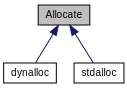
\includegraphics[width=200pt]{class_allocate__inherit__graph}
\end{center}
\end{figure}


Collaboration diagram for Allocate\+:
\nopagebreak
\begin{figure}[H]
\begin{center}
\leavevmode
\includegraphics[width=323pt]{class_allocate__coll__graph}
\end{center}
\end{figure}
\subsection*{Public Member Functions}
\begin{DoxyCompactItemize}
\item 
\hyperlink{class_allocate_ab2b82e7fab9d0fccb9702effec93917b}{Allocate} (\hyperlink{classraft_1_1map}{raft\+::map} \&map, volatile bool \&\hyperlink{class_allocate_a4d10076b88ab1297c89b8a05e117b510}{exit\+\_\+alloc})
\item 
virtual \hyperlink{class_allocate_a68cd61da26f3b82da094b6d3e5d556f5}{$\sim$\+Allocate} ()
\item 
virtual void \hyperlink{class_allocate_a44f9b51c382fec159233609e21b9d272}{run} ()=0
\item 
void \hyperlink{class_allocate_a3123c2c1d9584974ce19b47fe6ceea17}{wait\+Till\+Ready} ()
\end{DoxyCompactItemize}
\subsection*{Protected Member Functions}
\begin{DoxyCompactItemize}
\item 
void \hyperlink{class_allocate_a1d5c71b5cd6fc9671ed82d9c1d04965c}{initialize} (\hyperlink{struct_port_info}{Port\+Info} $\ast$const src, \hyperlink{struct_port_info}{Port\+Info} $\ast$const dst, \hyperlink{class_f_i_f_o}{F\+I\+FO} $\ast$const fifo)
\item 
\hypertarget{class_allocate_a901eb0fdb6cffd56019c9ab9f2b25f92}{}\label{class_allocate_a901eb0fdb6cffd56019c9ab9f2b25f92} 
virtual void {\bfseries allocate} (\hyperlink{struct_port_info}{Port\+Info} \&a, \hyperlink{struct_port_info}{Port\+Info} \&b, void $\ast$data)
\item 
void \hyperlink{class_allocate_a4cf36bb704e43f5736a0e736d9e1a81b}{set\+Ready} ()
\end{DoxyCompactItemize}
\subsection*{Protected Attributes}
\begin{DoxyCompactItemize}
\item 
kernelkeeper \& \hyperlink{class_allocate_a93e612d7ea7eb686fc88b5dee7a1407b}{source\+\_\+kernels}
\item 
\hypertarget{class_allocate_a91e8c7d69ab7b309ea45439aea54fb4f}{}\label{class_allocate_a91e8c7d69ab7b309ea45439aea54fb4f} 
kernelkeeper \& {\bfseries all\+\_\+kernels}
\item 
std\+::set$<$ \hyperlink{class_f_i_f_o}{F\+I\+FO} $\ast$$>$ \hyperlink{class_allocate_a037410210c0d10578f87de1ec68f47ba}{allocated\+\_\+fifo}
\item 
volatile bool \& \hyperlink{class_allocate_a4d10076b88ab1297c89b8a05e117b510}{exit\+\_\+alloc}
\end{DoxyCompactItemize}
\subsection*{Friends}
\begin{DoxyCompactItemize}
\item 
\hypertarget{class_allocate_a901ac6fe1c35f3c114cf9e83f75dde0c}{}\label{class_allocate_a901ac6fe1c35f3c114cf9e83f75dde0c} 
class {\bfseries basic\+\_\+parallel}
\end{DoxyCompactItemize}


\subsection{Detailed Description}


Definition at line 58 of file allocate.\+hpp.



\subsection{Constructor \& Destructor Documentation}
\hypertarget{class_allocate_ab2b82e7fab9d0fccb9702effec93917b}{}\label{class_allocate_ab2b82e7fab9d0fccb9702effec93917b} 
\index{Allocate@{Allocate}!Allocate@{Allocate}}
\index{Allocate@{Allocate}!Allocate@{Allocate}}
\subsubsection{\texorpdfstring{Allocate()}{Allocate()}}
{\footnotesize\ttfamily Allocate\+::\+Allocate (\begin{DoxyParamCaption}\item[{\hyperlink{classraft_1_1map}{raft\+::map} \&}]{map,  }\item[{volatile bool \&}]{exit\+\_\+alloc }\end{DoxyParamCaption})}

\hyperlink{class_allocate}{Allocate} -\/ base constructor, really doesn\textquotesingle{}t do too much save for setting the global variables all\+\_\+kernels and source\+\_\+kernels from the Map object. 
\begin{DoxyParams}{Parameters}
{\em map} & -\/ \hyperlink{classraft_1_1map}{raft\+::map}\& \\
\hline
{\em exit\+\_\+alloc} & -\/ bool used to terminate loop, for monitoring allocations, controlled by map object.\\
\hline
\end{DoxyParams}
allocate.\+cpp -\/ \begin{DoxyAuthor}{Author}
\+: Jonathan Beard 
\end{DoxyAuthor}
\begin{DoxyVersion}{Version}
\+: Tue Sep 16 20\+:20\+:06 2014
\end{DoxyVersion}
Copyright 2014 Jonathan Beard

Licensed under the Apache License, Version 2.\+0 (the \char`\"{}\+License\char`\"{}); you may not use this file except in compliance with the License. You may obtain a copy of the License at\+:

\href{http://www.apache.org/licenses/LICENSE-2.0}{\tt http\+://www.\+apache.\+org/licenses/\+L\+I\+C\+E\+N\+S\+E-\/2.\+0}

Unless required by applicable law or agreed to in writing, software distributed under the License is distributed on an \char`\"{}\+A\+S I\+S\char`\"{} B\+A\+S\+IS, W\+I\+T\+H\+O\+UT W\+A\+R\+R\+A\+N\+T\+I\+ES OR C\+O\+N\+D\+I\+T\+I\+O\+NS OF A\+NY K\+I\+ND, either express or implied. See the License for the specific language governing permissions and limitations under the License. 

Definition at line 30 of file src/allocate.\+cpp.


\begin{DoxyCode}
30                                                             :
31    \hyperlink{class_allocate_a93e612d7ea7eb686fc88b5dee7a1407b}{source\_kernels}( map.\hyperlink{class_map_base_a2541cb37a237e66fc88129f9f0b02f50}{source\_kernels} ),
32    all\_kernels(    map.\hyperlink{class_map_base_a2220cd630c5d00708f08d9bc70a48220}{all\_kernels} ),
33    \hyperlink{class_allocate_a4d10076b88ab1297c89b8a05e117b510}{exit\_alloc}( \hyperlink{class_allocate_a4d10076b88ab1297c89b8a05e117b510}{exit\_alloc} )
34 \{
35 \}
\end{DoxyCode}
\hypertarget{class_allocate_a68cd61da26f3b82da094b6d3e5d556f5}{}\label{class_allocate_a68cd61da26f3b82da094b6d3e5d556f5} 
\index{Allocate@{Allocate}!````~Allocate@{$\sim$\+Allocate}}
\index{````~Allocate@{$\sim$\+Allocate}!Allocate@{Allocate}}
\subsubsection{\texorpdfstring{$\sim$\+Allocate()}{~Allocate()}}
{\footnotesize\ttfamily Allocate\+::$\sim$\+Allocate (\begin{DoxyParamCaption}{ }\end{DoxyParamCaption})\hspace{0.3cm}{\ttfamily [virtual]}}

destructor 

Definition at line 37 of file src/allocate.\+cpp.



References allocated\+\_\+fifo.


\begin{DoxyCode}
38 \{
39    \textcolor{keywordflow}{for}( \hyperlink{class_f_i_f_o}{FIFO} *f : \hyperlink{class_allocate_a037410210c0d10578f87de1ec68f47ba}{allocated\_fifo} )
40    \{
41       \textcolor{keyword}{delete}( f );
42    \}
43 \}
\end{DoxyCode}


\subsection{Member Function Documentation}
\hypertarget{class_allocate_a1d5c71b5cd6fc9671ed82d9c1d04965c}{}\label{class_allocate_a1d5c71b5cd6fc9671ed82d9c1d04965c} 
\index{Allocate@{Allocate}!initialize@{initialize}}
\index{initialize@{initialize}!Allocate@{Allocate}}
\subsubsection{\texorpdfstring{initialize()}{initialize()}}
{\footnotesize\ttfamily void Allocate\+::initialize (\begin{DoxyParamCaption}\item[{\hyperlink{struct_port_info}{Port\+Info} $\ast$const}]{src,  }\item[{\hyperlink{struct_port_info}{Port\+Info} $\ast$const}]{dst,  }\item[{\hyperlink{class_f_i_f_o}{F\+I\+FO} $\ast$const}]{fifo }\end{DoxyParamCaption})\hspace{0.3cm}{\ttfamily [protected]}}

initialize -\/ internal method to be used within the run method takes care of the initialization using the already allocated \hyperlink{class_f_i_f_o}{F\+I\+FO} object passed as a param. This function will throw an exception if either port (src or dst) have already been allocated. 
\begin{DoxyParams}{Parameters}
{\em src} & -\/ Port\+Info$\ast$, nullptr if not to be set \\
\hline
{\em dst} & -\/ Port\+Info$\ast$, nullptr if not to be set \\
\hline
{\em fifo} & -\/ F\+I\+F\+O$\ast$ \\
\hline
\end{DoxyParams}

\begin{DoxyExceptions}{Exceptions}
{\em \hyperlink{class_port_double_initialize_exception}{Port\+Double\+Initialize\+Exception}} & -\/ if either port is already initialized. \\
\hline
\end{DoxyExceptions}
N\+O\+TE\+: this list simply speeds up the monitoring if we want it 

Definition at line 58 of file src/allocate.\+cpp.



References allocated\+\_\+fifo, Port\+Info\+::const\+\_\+map, Port\+Info\+::get\+F\+I\+F\+O(), F\+I\+F\+O\+::set\+\_\+dst\+\_\+kernel(), F\+I\+F\+O\+::set\+\_\+src\+\_\+kernel(), and Port\+Info\+::set\+F\+I\+F\+O().



Referenced by stdalloc\+::run().


\begin{DoxyCode}
61 \{
62    assert( fifo != \textcolor{keyword}{nullptr} );
63    assert( dst  != \textcolor{keyword}{nullptr} );
64    assert( src  != \textcolor{keyword}{nullptr} );
65    \textcolor{keywordflow}{if}( src->\hyperlink{struct_port_info_a483d162fbe356e07381c6c5cfccb4f48}{getFIFO}() != nullptr )
66    \{
67       \textcolor{keywordflow}{throw} \hyperlink{class_port_double_initialize_exception}{PortDoubleInitializeException}(
68          \textcolor{stringliteral}{"Source port \(\backslash\)""} + src->my\_name + \textcolor{stringliteral}{"\(\backslash\)" already initialized!"} );
69    \}
70    \textcolor{keywordflow}{if}( dst->\hyperlink{struct_port_info_a483d162fbe356e07381c6c5cfccb4f48}{getFIFO}() !=  nullptr )
71    \{
72       \textcolor{keywordflow}{throw} \hyperlink{class_port_double_initialize_exception}{PortDoubleInitializeException}(
73          \textcolor{stringliteral}{"Destination port \(\backslash\)""} + dst->my\_name +  \textcolor{stringliteral}{"\(\backslash\)" already initialized!"} );
74    \}
75    src->\hyperlink{struct_port_info_a43a57cd624dcc44ccd9dcaba1d07a000}{setFIFO}( fifo );
76    fifo->\hyperlink{class_f_i_f_o_aa9c1f679b4e2585047af2c09a2518209}{set\_src\_kernel}( src->my\_kernel );
77    dst->\hyperlink{struct_port_info_a43a57cd624dcc44ccd9dcaba1d07a000}{setFIFO}( fifo );
78    fifo->\hyperlink{class_f_i_f_o_a11422695c75c05ad2c60e662553f2667}{set\_dst\_kernel}( dst->my\_kernel );\textcolor{comment}{}
79 \textcolor{comment}{   /** NOTE: this list simply speeds up the monitoring if we want it **/}
80    \hyperlink{class_allocate_a037410210c0d10578f87de1ec68f47ba}{allocated\_fifo}.insert( fifo );
81 \}
\end{DoxyCode}
Here is the call graph for this function\+:
\nopagebreak
\begin{figure}[H]
\begin{center}
\leavevmode
\includegraphics[width=318pt]{class_allocate_a1d5c71b5cd6fc9671ed82d9c1d04965c_cgraph}
\end{center}
\end{figure}
\hypertarget{class_allocate_a44f9b51c382fec159233609e21b9d272}{}\label{class_allocate_a44f9b51c382fec159233609e21b9d272} 
\index{Allocate@{Allocate}!run@{run}}
\index{run@{run}!Allocate@{Allocate}}
\subsubsection{\texorpdfstring{run()}{run()}}
{\footnotesize\ttfamily virtual void Allocate\+::run (\begin{DoxyParamCaption}{ }\end{DoxyParamCaption})\hspace{0.3cm}{\ttfamily [pure virtual]}}

run -\/ implement this function to create a new allocator, will be run inside a thread so exits when done but if run-\/time monitoring is desired then this is the place to do it. 

Implemented in \hyperlink{classstdalloc_a60438b15948ce354b52b03ba6d975de0}{stdalloc}, and \hyperlink{classdynalloc_a2a52b86ec09bd6dd52e49062137b2e37}{dynalloc}.

\hypertarget{class_allocate_a4cf36bb704e43f5736a0e736d9e1a81b}{}\label{class_allocate_a4cf36bb704e43f5736a0e736d9e1a81b} 
\index{Allocate@{Allocate}!set\+Ready@{set\+Ready}}
\index{set\+Ready@{set\+Ready}!Allocate@{Allocate}}
\subsubsection{\texorpdfstring{set\+Ready()}{setReady()}}
{\footnotesize\ttfamily void Allocate\+::set\+Ready (\begin{DoxyParamCaption}{ }\end{DoxyParamCaption})\hspace{0.3cm}{\ttfamily [protected]}}

set\+Ready -\/ call within the implemented run function to signal that the initial allocations have been completed. 

Definition at line 52 of file src/allocate.\+cpp.



Referenced by dynalloc\+::run(), and stdalloc\+::run().


\begin{DoxyCode}
53 \{
54    ready = \textcolor{keyword}{true};
55 \}
\end{DoxyCode}
\hypertarget{class_allocate_a3123c2c1d9584974ce19b47fe6ceea17}{}\label{class_allocate_a3123c2c1d9584974ce19b47fe6ceea17} 
\index{Allocate@{Allocate}!wait\+Till\+Ready@{wait\+Till\+Ready}}
\index{wait\+Till\+Ready@{wait\+Till\+Ready}!Allocate@{Allocate}}
\subsubsection{\texorpdfstring{wait\+Till\+Ready()}{waitTillReady()}}
{\footnotesize\ttfamily void Allocate\+::wait\+Till\+Ready (\begin{DoxyParamCaption}{ }\end{DoxyParamCaption})}

wait\+Till\+Ready -\/ call after initializing the allocate thread, returns when the initial allocation is complete. 

Definition at line 46 of file src/allocate.\+cpp.


\begin{DoxyCode}
47 \{
48    \textcolor{keywordflow}{while}( ! ready );
49 \}
\end{DoxyCode}


\subsection{Member Data Documentation}
\hypertarget{class_allocate_a037410210c0d10578f87de1ec68f47ba}{}\label{class_allocate_a037410210c0d10578f87de1ec68f47ba} 
\index{Allocate@{Allocate}!allocated\+\_\+fifo@{allocated\+\_\+fifo}}
\index{allocated\+\_\+fifo@{allocated\+\_\+fifo}!Allocate@{Allocate}}
\subsubsection{\texorpdfstring{allocated\+\_\+fifo}{allocated\_fifo}}
{\footnotesize\ttfamily std\+::set$<$ \hyperlink{class_f_i_f_o}{F\+I\+FO}$\ast$ $>$ Allocate\+::allocated\+\_\+fifo\hspace{0.3cm}{\ttfamily [protected]}}

keeps a list of all currently allocated \hyperlink{class_f_i_f_o}{F\+I\+FO} objects, set from within the initialize function. 

Definition at line 124 of file allocate.\+hpp.



Referenced by initialize(), and $\sim$\+Allocate().

\hypertarget{class_allocate_a4d10076b88ab1297c89b8a05e117b510}{}\label{class_allocate_a4d10076b88ab1297c89b8a05e117b510} 
\index{Allocate@{Allocate}!exit\+\_\+alloc@{exit\+\_\+alloc}}
\index{exit\+\_\+alloc@{exit\+\_\+alloc}!Allocate@{Allocate}}
\subsubsection{\texorpdfstring{exit\+\_\+alloc}{exit\_alloc}}
{\footnotesize\ttfamily volatile bool\& Allocate\+::exit\+\_\+alloc\hspace{0.3cm}{\ttfamily [protected]}}

exit\+\_\+alloc -\/ bool whose value is set by the map object, controls when the loop within the alloc thread is exited. 

Definition at line 131 of file allocate.\+hpp.



Referenced by dynalloc\+::run().

\hypertarget{class_allocate_a93e612d7ea7eb686fc88b5dee7a1407b}{}\label{class_allocate_a93e612d7ea7eb686fc88b5dee7a1407b} 
\index{Allocate@{Allocate}!source\+\_\+kernels@{source\+\_\+kernels}}
\index{source\+\_\+kernels@{source\+\_\+kernels}!Allocate@{Allocate}}
\subsubsection{\texorpdfstring{source\+\_\+kernels}{source\_kernels}}
{\footnotesize\ttfamily kernelkeeper\& Allocate\+::source\+\_\+kernels\hspace{0.3cm}{\ttfamily [protected]}}

both convenience structs, hold exactly what the names say 

Definition at line 117 of file allocate.\+hpp.



Referenced by dynalloc\+::run(), and stdalloc\+::run().



The documentation for this class was generated from the following files\+:\begin{DoxyCompactItemize}
\item 
allocate.\+hpp\item 
src/allocate.\+cpp\end{DoxyCompactItemize}

\hypertarget{class_ambiguous_port_assignment_exception}{}\section{Ambiguous\+Port\+Assignment\+Exception Class Reference}
\label{class_ambiguous_port_assignment_exception}\index{Ambiguous\+Port\+Assignment\+Exception@{Ambiguous\+Port\+Assignment\+Exception}}
Inheritance diagram for Ambiguous\+Port\+Assignment\+Exception\+:\begin{figure}[H]
\begin{center}
\leavevmode
\includegraphics[height=3.000000cm]{class_ambiguous_port_assignment_exception}
\end{center}
\end{figure}
\subsection*{Public Member Functions}
\begin{DoxyCompactItemize}
\item 
\hypertarget{class_ambiguous_port_assignment_exception_a5c2daf243080521a90629fcc262dec61}{}{\bfseries Ambiguous\+Port\+Assignment\+Exception} (const std\+::string message)\label{class_ambiguous_port_assignment_exception_a5c2daf243080521a90629fcc262dec61}

\end{DoxyCompactItemize}


The documentation for this class was generated from the following files\+:\begin{DoxyCompactItemize}
\item 
portexception.\+hpp\item 
portexception.\+cpp\end{DoxyCompactItemize}

\hypertarget{structautopair}{}\section{autopair$<$ T $>$ Struct Template Reference}
\label{structautopair}\index{autopair$<$ T $>$@{autopair$<$ T $>$}}


{\ttfamily \#include $<$autoreleasebase.\+hpp$>$}



Collaboration diagram for autopair$<$ T $>$\+:
\nopagebreak
\begin{figure}[H]
\begin{center}
\leavevmode
\includegraphics[width=219pt]{structautopair__coll__graph}
\end{center}
\end{figure}
\subsection*{Public Member Functions}
\begin{DoxyCompactItemize}
\item 
\hypertarget{structautopair_a1d2579cf46990324db585e503b7d1e2b}{}\label{structautopair_a1d2579cf46990324db585e503b7d1e2b} 
{\bfseries autopair} (T \&ele, \hyperlink{struct_buffer_1_1_signal}{Buffer\+::\+Signal} \&sig)
\end{DoxyCompactItemize}
\subsection*{Public Attributes}
\begin{DoxyCompactItemize}
\item 
\hypertarget{structautopair_a689ed2b7027d53831ea76d0131bd416f}{}\label{structautopair_a689ed2b7027d53831ea76d0131bd416f} 
T \& {\bfseries ele}
\item 
\hypertarget{structautopair_a5c4e5b72c053a2606e3cc4b3cb7b8b88}{}\label{structautopair_a5c4e5b72c053a2606e3cc4b3cb7b8b88} 
\hyperlink{struct_buffer_1_1_signal}{Buffer\+::\+Signal} \& {\bfseries sig}
\end{DoxyCompactItemize}


\subsection{Detailed Description}
\subsubsection*{template$<$class T$>$\newline
struct autopair$<$ T $>$}

\hyperlink{autoreleasebase_8hpp_source}{autoreleasebase.\+hpp} -\/ \begin{DoxyAuthor}{Author}
\+: Jonathan Beard 
\end{DoxyAuthor}
\begin{DoxyVersion}{Version}
\+: Thu Aug 27 14\+:24\+:31 2015
\end{DoxyVersion}
Copyright 2015 Jonathan Beard

Licensed under the Apache License, Version 2.\+0 (the \char`\"{}\+License\char`\"{}); you may not use this file except in compliance with the License. You may obtain a copy of the License at\+:

\href{http://www.apache.org/licenses/LICENSE-2.0}{\tt http\+://www.\+apache.\+org/licenses/\+L\+I\+C\+E\+N\+S\+E-\/2.\+0}

Unless required by applicable law or agreed to in writing, software distributed under the License is distributed on an \char`\"{}\+A\+S I\+S\char`\"{} B\+A\+S\+IS, W\+I\+T\+H\+O\+UT W\+A\+R\+R\+A\+N\+T\+I\+ES OR C\+O\+N\+D\+I\+T\+I\+O\+NS OF A\+NY K\+I\+ND, either express or implied. See the License for the specific language governing permissions and limitations under the License. this is used by the autorelease objects so that index operator \mbox{[}\mbox{]} can return access to both the signal and the element at that index 

Definition at line 27 of file autoreleasebase.\+hpp.



The documentation for this struct was generated from the following file\+:\begin{DoxyCompactItemize}
\item 
autoreleasebase.\+hpp\end{DoxyCompactItemize}

\hypertarget{classautoreleasebase}{}\section{autoreleasebase Class Reference}
\label{classautoreleasebase}\index{autoreleasebase@{autoreleasebase}}


\subsection{Detailed Description}


Definition at line 37 of file autoreleasebase.\+hpp.



The documentation for this class was generated from the following file\+:\begin{DoxyCompactItemize}
\item 
autoreleasebase.\+hpp\end{DoxyCompactItemize}

\hypertarget{classbasic__parallel}{}\section{basic\+\_\+parallel Class Reference}
\label{classbasic__parallel}\index{basic\+\_\+parallel@{basic\+\_\+parallel}}
\subsection*{Public Member Functions}
\begin{DoxyCompactItemize}
\item 
\hyperlink{classbasic__parallel_a6f8a4933fb29d6f4c60ebb3e934b192e}{basic\+\_\+parallel} (\hyperlink{class_map}{Map} \&map, \hyperlink{class_allocate}{Allocate} \&alloc, \hyperlink{class_schedule}{Schedule} \&sched, volatile bool \&exit\+\_\+para)
\item 
virtual void \hyperlink{classbasic__parallel_a85ea2560d40ad50482468e39d626a52b}{start} ()
\end{DoxyCompactItemize}
\subsection*{Protected Attributes}
\begin{DoxyCompactItemize}
\item 
kernelkeeper \& \hyperlink{classbasic__parallel_a969b8832b2f6eaea5e985d4582d9e4dc}{source\+\_\+kernels}
\item 
\hypertarget{classbasic__parallel_a028feb03732d5fef0e9d184ddc18ce7b}{}kernelkeeper \& {\bfseries all\+\_\+kernels}\label{classbasic__parallel_a028feb03732d5fef0e9d184ddc18ce7b}

\item 
\hypertarget{classbasic__parallel_aab09daae41a9d218568115be037a8357}{}\hyperlink{class_allocate}{Allocate} \& {\bfseries alloc}\label{classbasic__parallel_aab09daae41a9d218568115be037a8357}

\item 
\hypertarget{classbasic__parallel_a9124d0bfd5d75277ddd44fb59814435a}{}\hyperlink{class_schedule}{Schedule} \& {\bfseries sched}\label{classbasic__parallel_a9124d0bfd5d75277ddd44fb59814435a}

\item 
\hypertarget{classbasic__parallel_ac648d03dceed09e7834d656f561da33b}{}volatile bool \& {\bfseries exit\+\_\+para}\label{classbasic__parallel_ac648d03dceed09e7834d656f561da33b}

\end{DoxyCompactItemize}


\subsection{Constructor \& Destructor Documentation}
\hypertarget{classbasic__parallel_a6f8a4933fb29d6f4c60ebb3e934b192e}{}\index{basic\+\_\+parallel@{basic\+\_\+parallel}!basic\+\_\+parallel@{basic\+\_\+parallel}}
\index{basic\+\_\+parallel@{basic\+\_\+parallel}!basic\+\_\+parallel@{basic\+\_\+parallel}}
\subsubsection[{basic\+\_\+parallel(\+Map \&map, Allocate \&alloc, Schedule \&sched, volatile bool \&exit\+\_\+para)}]{\setlength{\rightskip}{0pt plus 5cm}basic\+\_\+parallel\+::basic\+\_\+parallel (
\begin{DoxyParamCaption}
\item[{{\bf Map} \&}]{map, }
\item[{{\bf Allocate} \&}]{alloc, }
\item[{{\bf Schedule} \&}]{sched, }
\item[{volatile bool \&}]{exit\+\_\+para}
\end{DoxyParamCaption}
)}\label{classbasic__parallel_a6f8a4933fb29d6f4c60ebb3e934b192e}
nothing to do here, move along 

\subsection{Member Function Documentation}
\hypertarget{classbasic__parallel_a85ea2560d40ad50482468e39d626a52b}{}\index{basic\+\_\+parallel@{basic\+\_\+parallel}!start@{start}}
\index{start@{start}!basic\+\_\+parallel@{basic\+\_\+parallel}}
\subsubsection[{start()}]{\setlength{\rightskip}{0pt plus 5cm}void basic\+\_\+parallel\+::start (
\begin{DoxyParamCaption}
{}
\end{DoxyParamCaption}
)\hspace{0.3cm}{\ttfamily [virtual]}}\label{classbasic__parallel_a85ea2560d40ad50482468e39d626a52b}
since we have to have a lock on the ports for both B\+F\+S and duplication, we\textquotesingle{}ll mark the kernels inside of B\+F\+S and duplicate outside of it.

start checking stats

input stats

apply criteria

F\+I\+X\+M\+E, logic below only works for single input, single output..intended to get it working

clone

attach ports

connecting a.\+y -\/$>$ b.\+x new\+\_\+other\+\_\+outprt == port y on a new\+\_\+port\+\_\+in == port x on b

connecting b.\+y -\/$>$ c.\+x newoutport == port y on b new\+\_\+other\+\_\+inport == port x on c

schedule new kernel 

\subsection{Member Data Documentation}
\hypertarget{classbasic__parallel_a969b8832b2f6eaea5e985d4582d9e4dc}{}\index{basic\+\_\+parallel@{basic\+\_\+parallel}!source\+\_\+kernels@{source\+\_\+kernels}}
\index{source\+\_\+kernels@{source\+\_\+kernels}!basic\+\_\+parallel@{basic\+\_\+parallel}}
\subsubsection[{source\+\_\+kernels}]{\setlength{\rightskip}{0pt plus 5cm}kernelkeeper\& basic\+\_\+parallel\+::source\+\_\+kernels\hspace{0.3cm}{\ttfamily [protected]}}\label{classbasic__parallel_a969b8832b2f6eaea5e985d4582d9e4dc}
both convenience structs, hold exactly what the names say 

The documentation for this class was generated from the following files\+:\begin{DoxyCompactItemize}
\item 
basicparallel.\+hpp\item 
basicparallel.\+cpp\end{DoxyCompactItemize}

\hypertarget{struct_blocked}{}\section{Blocked Struct Reference}
\label{struct_blocked}\index{Blocked@{Blocked}}


{\ttfamily \#include $<$blocked.\+hpp$>$}



Collaboration diagram for Blocked\+:
\nopagebreak
\begin{figure}[H]
\begin{center}
\leavevmode
\includegraphics[width=350pt]{struct_blocked__coll__graph}
\end{center}
\end{figure}
\subsection*{Classes}
\begin{DoxyCompactItemize}
\item 
struct \hyperlink{struct_blocked_1_1blocked__and__counter}{blocked\+\_\+and\+\_\+counter}
\end{DoxyCompactItemize}
\subsection*{Public Types}
\begin{DoxyCompactItemize}
\item 
\hypertarget{struct_blocked_a5c1d9f4d77e4940785c83a43ce81729f}{}\label{struct_blocked_a5c1d9f4d77e4940785c83a43ce81729f} 
using {\bfseries value\+\_\+type} = std\+::uint32\+\_\+t
\item 
\hypertarget{struct_blocked_a0b0291787b8f79d99ae9a60ad84cd3e0}{}\label{struct_blocked_a0b0291787b8f79d99ae9a60ad84cd3e0} 
using {\bfseries whole\+\_\+type} = std\+::uint64\+\_\+t
\end{DoxyCompactItemize}
\subsection*{Public Member Functions}
\begin{DoxyCompactItemize}
\item 
\hypertarget{struct_blocked_aab6ec9e4b1fd78fa02c50db7d3c1d623}{}\label{struct_blocked_aab6ec9e4b1fd78fa02c50db7d3c1d623} 
{\bfseries Blocked} (const \hyperlink{struct_blocked}{Blocked} \&other)
\item 
\hypertarget{struct_blocked_afe38f1192d5feef760dc1992fdd0bef4}{}\label{struct_blocked_afe38f1192d5feef760dc1992fdd0bef4} 
\hyperlink{struct_blocked}{Blocked} \& {\bfseries operator+=} (const \hyperlink{struct_blocked}{Blocked} \&rhs)
\end{DoxyCompactItemize}
\subsection*{Public Attributes}
\begin{DoxyCompactItemize}
\item 
\hypertarget{struct_blocked_a8a4071ed2ac86920e4fcd21bc39cae48}{}\label{struct_blocked_a8a4071ed2ac86920e4fcd21bc39cae48} 
\begin{tabbing}
xx\=xx\=xx\=xx\=xx\=xx\=xx\=xx\=xx\=\kill
union \{\\
\>\hyperlink{struct_blocked_1_1blocked__and__counter}{blocked\_and\_counter} {\bfseries bec}\\
\>whole\_type {\bfseries all} = 0\\
\}; \\

\end{tabbing}\item 
\hypertarget{struct_blocked_a655f1539c05155f99a1b016331a89b90}{}\label{struct_blocked_a655f1539c05155f99a1b016331a89b90} 
char {\bfseries pad} \mbox{[}L1\+D\+\_\+\+C\+A\+C\+H\+E\+\_\+\+L\+I\+N\+E\+\_\+\+S\+I\+ZE -\/ sizeof(whole\+\_\+type)\mbox{]}
\end{DoxyCompactItemize}


\subsection{Detailed Description}
\hyperlink{blocked_8hpp_source}{blocked.\+hpp} -\/ \begin{DoxyAuthor}{Author}
\+: Jonathan Beard 
\end{DoxyAuthor}
\begin{DoxyVersion}{Version}
\+: Sun Jun 29 14\+:06\+:10 2014
\end{DoxyVersion}
Copyright 2014 Jonathan Beard

Licensed under the Apache License, Version 2.\+0 (the \char`\"{}\+License\char`\"{}); you may not use this file except in compliance with the License. You may obtain a copy of the License at\+:

\href{http://www.apache.org/licenses/LICENSE-2.0}{\tt http\+://www.\+apache.\+org/licenses/\+L\+I\+C\+E\+N\+S\+E-\/2.\+0}

Unless required by applicable law or agreed to in writing, software distributed under the License is distributed on an \char`\"{}\+A\+S I\+S\char`\"{} B\+A\+S\+IS, W\+I\+T\+H\+O\+UT W\+A\+R\+R\+A\+N\+T\+I\+ES OR C\+O\+N\+D\+I\+T\+I\+O\+NS OF A\+NY K\+I\+ND, either express or implied. See the License for the specific language governing permissions and limitations under the License. F\+I\+X\+ME...should probably align these to cache line then zero extend pad for producer/consumer. 

Definition at line 29 of file blocked.\+hpp.



The documentation for this struct was generated from the following file\+:\begin{DoxyCompactItemize}
\item 
blocked.\+hpp\end{DoxyCompactItemize}

\hypertarget{struct_blocked_1_1blocked__and__counter}{}\section{Blocked\+:\+:blocked\+\_\+and\+\_\+counter Struct Reference}
\label{struct_blocked_1_1blocked__and__counter}\index{Blocked\+::blocked\+\_\+and\+\_\+counter@{Blocked\+::blocked\+\_\+and\+\_\+counter}}


Collaboration diagram for Blocked\+:\+:blocked\+\_\+and\+\_\+counter\+:
\nopagebreak
\begin{figure}[H]
\begin{center}
\leavevmode
\includegraphics[width=194pt]{struct_blocked_1_1blocked__and__counter__coll__graph}
\end{center}
\end{figure}
\subsection*{Public Attributes}
\begin{DoxyCompactItemize}
\item 
\hypertarget{struct_blocked_1_1blocked__and__counter_adbdd8f50a31d16dab89bc0525881cbb5}{}\label{struct_blocked_1_1blocked__and__counter_adbdd8f50a31d16dab89bc0525881cbb5} 
value\+\_\+type {\bfseries blocked}
\item 
\hypertarget{struct_blocked_1_1blocked__and__counter_a926f029d3834d74776188aaf4aa8de7c}{}\label{struct_blocked_1_1blocked__and__counter_a926f029d3834d74776188aaf4aa8de7c} 
value\+\_\+type {\bfseries count}
\end{DoxyCompactItemize}


\subsection{Detailed Description}


Definition at line 48 of file blocked.\+hpp.



The documentation for this struct was generated from the following file\+:\begin{DoxyCompactItemize}
\item 
blocked.\+hpp\end{DoxyCompactItemize}

\hypertarget{class_clone_not_implemented_exception}{}\section{Clone\+Not\+Implemented\+Exception Class Reference}
\label{class_clone_not_implemented_exception}\index{Clone\+Not\+Implemented\+Exception@{Clone\+Not\+Implemented\+Exception}}


Inheritance diagram for Clone\+Not\+Implemented\+Exception\+:
\nopagebreak
\begin{figure}[H]
\begin{center}
\leavevmode
\includegraphics[width=239pt]{class_clone_not_implemented_exception__inherit__graph}
\end{center}
\end{figure}


Collaboration diagram for Clone\+Not\+Implemented\+Exception\+:
\nopagebreak
\begin{figure}[H]
\begin{center}
\leavevmode
\includegraphics[width=239pt]{class_clone_not_implemented_exception__coll__graph}
\end{center}
\end{figure}
\subsection*{Public Member Functions}
\begin{DoxyCompactItemize}
\item 
\hypertarget{class_clone_not_implemented_exception_a079b0f22e6fc12f2bdd7fa10dd906c3a}{}\label{class_clone_not_implemented_exception_a079b0f22e6fc12f2bdd7fa10dd906c3a} 
{\bfseries Clone\+Not\+Implemented\+Exception} (const std\+::string message)
\end{DoxyCompactItemize}


\subsection{Detailed Description}


Definition at line 34 of file kernelexception.\+hpp.



The documentation for this class was generated from the following file\+:\begin{DoxyCompactItemize}
\item 
kernelexception.\+hpp\end{DoxyCompactItemize}

\hypertarget{class_closed_port_access_exception}{}\section{Closed\+Port\+Access\+Exception Class Reference}
\label{class_closed_port_access_exception}\index{Closed\+Port\+Access\+Exception@{Closed\+Port\+Access\+Exception}}


Inheritance diagram for Closed\+Port\+Access\+Exception\+:
\nopagebreak
\begin{figure}[H]
\begin{center}
\leavevmode
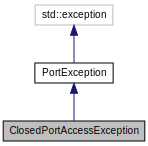
\includegraphics[width=222pt]{class_closed_port_access_exception__inherit__graph}
\end{center}
\end{figure}


Collaboration diagram for Closed\+Port\+Access\+Exception\+:
\nopagebreak
\begin{figure}[H]
\begin{center}
\leavevmode
\includegraphics[width=222pt]{class_closed_port_access_exception__coll__graph}
\end{center}
\end{figure}
\subsection*{Public Member Functions}
\begin{DoxyCompactItemize}
\item 
\hypertarget{class_closed_port_access_exception_aa66df922ca194ecd6431bd9cae0a4b24}{}\label{class_closed_port_access_exception_aa66df922ca194ecd6431bd9cae0a4b24} 
{\bfseries Closed\+Port\+Access\+Exception} (const std\+::string message)
\end{DoxyCompactItemize}


\subsection{Detailed Description}


Definition at line 63 of file portexception.\+hpp.



The documentation for this class was generated from the following files\+:\begin{DoxyCompactItemize}
\item 
portexception.\+hpp\item 
portexception.\+cpp\end{DoxyCompactItemize}

\hypertarget{class_cmd_args}{}\section{Cmd\+Args Class Reference}
\label{class_cmd_args}\index{Cmd\+Args@{Cmd\+Args}}


{\ttfamily \#include $<$command\+\_\+arguments.\+h$>$}

\subsection*{Public Member Functions}
\begin{DoxyCompactItemize}
\item 
\hyperlink{class_cmd_args_a214efd9198eb8124a08e80cda9f0e253}{Cmd\+Args} (const std\+::string name, std\+::ostream \&user, std\+::ostream \&err)
\item 
void \hyperlink{class_cmd_args_aecdd9be22130abe064fb46a6ebc40c41}{print\+Args} ()
\item 
void \hyperlink{class_cmd_args_a1ac48d7334790086d8fb55e86d8cdd6e}{print\+Settings} ()
\item 
void \hyperlink{class_cmd_args_a58a223305551991a3b9f3a38d386295d}{add\+Option} (\hyperlink{class_option_base}{Option\+Base} $\ast$option)
\item 
void \hyperlink{class_cmd_args_a91066e5757db5cee24b244a736365939}{process\+Args} (int argc, char $\ast$$\ast$argv)
\item 
\hypertarget{class_cmd_args_a173bac3022d199a2973d76e9c93e4c88}{}\label{class_cmd_args_a173bac3022d199a2973d76e9c93e4c88} 
char $\ast$$\ast$ {\bfseries get\+Original\+Arguments} ()
\item 
\hypertarget{class_cmd_args_a7d53af33026586a5d0017297485f3aff}{}\label{class_cmd_args_a7d53af33026586a5d0017297485f3aff} 
int {\bfseries get\+Original\+Argument\+Count} ()
\item 
bool \hyperlink{class_cmd_args_af8460dc8b1ec7eb745d256f6e80afc2e}{all\+Mandatory\+Set} ()
\end{DoxyCompactItemize}


\subsection{Detailed Description}
\hyperlink{class_cmd_args}{Cmd\+Args} -\/ A very simple command line arguments src file, can be included in C++ and C files using the appropriate function calls. In order to use this to process your arguments simply do the following\+: //create a \hyperlink{class_cmd_args}{Cmd\+Args} object \hyperlink{class_cmd_args}{Cmd\+Args} $\ast$args = new \hyperlink{class_cmd_args}{Cmd\+Args(std\+::string(argv\mbox{[}0\mbox{]}))}; //sets program name for object //define static variables for options static bool my\+First\+Option = false; //assigning var gives default value //add options to \hyperlink{class_cmd_args}{Cmd\+Args} cmd-\/$>$add\+Option(new Option$<$bool$>$(\&my\+First\+Option,\char`\"{}-\/m\+F\+O\char`\"{},\char`\"{}\+An option\char`\"{})); //general form of cmd-\/$>$add\+Option(new Option$<$type$>$(var mem location, text flag, text description)); //give cmd line args to \hyperlink{class_cmd_args}{Cmd\+Args} cmd-\/$>$process\+Args(argc,argv) .....now you can use the variables as you see fit

\begin{DoxyAuthor}{Author}
Jonathan Beard 
\end{DoxyAuthor}
\begin{DoxyVersion}{Version}
Last modified 27 May 2012  \href{mailto:jbeard@wustl.edu}{\tt jbeard@wustl.\+edu} \hyperlink{class_cmd_args}{Cmd\+Args} -\/ actual cmd args class 
\end{DoxyVersion}


Definition at line 43 of file command\+\_\+arguments.\+h.



\subsection{Constructor \& Destructor Documentation}
\hypertarget{class_cmd_args_a214efd9198eb8124a08e80cda9f0e253}{}\label{class_cmd_args_a214efd9198eb8124a08e80cda9f0e253} 
\index{Cmd\+Args@{Cmd\+Args}!Cmd\+Args@{Cmd\+Args}}
\index{Cmd\+Args@{Cmd\+Args}!Cmd\+Args@{Cmd\+Args}}
\subsubsection{\texorpdfstring{Cmd\+Args()}{CmdArgs()}}
{\footnotesize\ttfamily Cmd\+Args\+::\+Cmd\+Args (\begin{DoxyParamCaption}\item[{const std\+::string}]{n,  }\item[{std\+::ostream \&}]{user,  }\item[{std\+::ostream \&}]{err }\end{DoxyParamCaption})}

Default Constructor -\/ 
\begin{DoxyParams}{Parameters}
{\em name} & -\/ std\+::string, name of program using \hyperlink{class_cmd_args}{Cmd\+Args} \\
\hline
{\em user} & -\/ std\+::ostream\&, stream for user output \\
\hline
{\em err} & -\/ std\+::ostream\&, stream for error output\\
\hline
\end{DoxyParams}
\hyperlink{class_cmd_args}{Cmd\+Args} -\/ A very simple command line arguments src file, can be included in C++ and C files using the appropriate function calls. In order to use this to process your arguments simply do the following\+: //create a \hyperlink{class_cmd_args}{Cmd\+Args} object \hyperlink{class_cmd_args}{Cmd\+Args} $\ast$args = new \hyperlink{class_cmd_args}{Cmd\+Args(std\+::string(argv\mbox{[}0\mbox{]}))}; //sets program name for object //define static variables for options static bool my\+First\+Option = false; //assigning var gives default value //add options to \hyperlink{class_cmd_args}{Cmd\+Args} cmd-\/$>$add\+Option(new Option$<$bool$>$(\&my\+First\+Option,\char`\"{}-\/m\+F\+O\char`\"{},\char`\"{}\+An option\char`\"{})); //general form of cmd-\/$>$add\+Option(new Option$<$type$>$(var mem location, text flag, text description)); //give cmd line args to \hyperlink{class_cmd_args}{Cmd\+Args} cmd-\/$>$process\+Args(argc,argv) .....now you can use the variables as you see fit

\begin{DoxyAuthor}{Author}
Jonathan Beard 
\end{DoxyAuthor}
\begin{DoxyVersion}{Version}
Last modified 27 May 2012  \href{mailto:jbeard@wustl.edu}{\tt jbeard@wustl.\+edu} 
\end{DoxyVersion}


Definition at line 34 of file command\+\_\+arguments.\+cpp.


\begin{DoxyCode}
37    : name( n ),
38      userstream( user ),
39      errorstream( err )
40 \{
41   \textcolor{comment}{/* nothing to do here, move along */}
42 \}
\end{DoxyCode}


\subsection{Member Function Documentation}
\hypertarget{class_cmd_args_a58a223305551991a3b9f3a38d386295d}{}\label{class_cmd_args_a58a223305551991a3b9f3a38d386295d} 
\index{Cmd\+Args@{Cmd\+Args}!add\+Option@{add\+Option}}
\index{add\+Option@{add\+Option}!Cmd\+Args@{Cmd\+Args}}
\subsubsection{\texorpdfstring{add\+Option()}{addOption()}}
{\footnotesize\ttfamily void Cmd\+Args\+::add\+Option (\begin{DoxyParamCaption}\item[{\hyperlink{class_option_base}{Option\+Base} $\ast$}]{option }\end{DoxyParamCaption})}

add\+Option -\/ each of these takes a ptr to an options object, there is a method for int64\+\_\+t, bool, std\+::string, and double. 

Definition at line 76 of file command\+\_\+arguments.\+cpp.


\begin{DoxyCode}
76                                     \{
77    assert( option != \textcolor{keyword}{nullptr} );
78    options.push\_back(option);
79 \}
\end{DoxyCode}
\hypertarget{class_cmd_args_af8460dc8b1ec7eb745d256f6e80afc2e}{}\label{class_cmd_args_af8460dc8b1ec7eb745d256f6e80afc2e} 
\index{Cmd\+Args@{Cmd\+Args}!all\+Mandatory\+Set@{all\+Mandatory\+Set}}
\index{all\+Mandatory\+Set@{all\+Mandatory\+Set}!Cmd\+Args@{Cmd\+Args}}
\subsubsection{\texorpdfstring{all\+Mandatory\+Set()}{allMandatorySet()}}
{\footnotesize\ttfamily bool Cmd\+Args\+::all\+Mandatory\+Set (\begin{DoxyParamCaption}{ }\end{DoxyParamCaption})}

not set yet

return false for rest, continue to print all not set 

Definition at line 148 of file command\+\_\+arguments.\+cpp.


\begin{DoxyCode}
149 \{
150    \textcolor{keywordtype}{bool} ret\_val( \textcolor{keyword}{true} );
151    \textcolor{keywordflow}{for}( \hyperlink{class_option_base}{OptionBase} * \textcolor{keyword}{const} option : options )
152    \{
153       assert( option != \textcolor{keyword}{nullptr} );
154       \textcolor{keywordflow}{if}( option->is\_mandatory() && ! option->is\_set() )
155       \{
156          \textcolor{keywordflow}{if}( ret\_val \textcolor{comment}{/** not set yet **/} )
157          \{
158            errorstream << \textcolor{stringliteral}{"\(\backslash\)033[1;36m"} << \textcolor{stringliteral}{"The following options must be set:"} << \textcolor{stringliteral}{"\(\backslash\)033[0m"} << \textcolor{stringliteral}{"\(\backslash\)n"};
159          \}
160          errorstream << \textcolor{stringliteral}{"\(\backslash\)033[1;31m"} << \textcolor{stringliteral}{"Option: "} << \textcolor{stringliteral}{"\(\backslash\)033[0m"} << option->toString() << \textcolor{stringliteral}{"\(\backslash\)n"}; \textcolor{comment}{}
161 \textcolor{comment}{         /** return false for rest, continue to print all not set **/}
162          ret\_val = \textcolor{keyword}{false};
163       \}
164    \}
165    \textcolor{keywordflow}{return}( ret\_val );
166 \}
\end{DoxyCode}
\hypertarget{class_cmd_args_aecdd9be22130abe064fb46a6ebc40c41}{}\label{class_cmd_args_aecdd9be22130abe064fb46a6ebc40c41} 
\index{Cmd\+Args@{Cmd\+Args}!print\+Args@{print\+Args}}
\index{print\+Args@{print\+Args}!Cmd\+Args@{Cmd\+Args}}
\subsubsection{\texorpdfstring{print\+Args()}{printArgs()}}
{\footnotesize\ttfamily void Cmd\+Args\+::print\+Args (\begin{DoxyParamCaption}{ }\end{DoxyParamCaption})}

print\+Args -\/ print all the options 

Definition at line 46 of file command\+\_\+arguments.\+cpp.


\begin{DoxyCode}
46                        \{
47    \textcolor{keywordtype}{char} stars[81];
48    generateStars( stars, 81 );
49    userstream << stars << std::endl;
50    userstream << \textcolor{stringliteral}{"Options menu for: "} << name << std::endl;
51    for\_each( options.begin(),
52              options.end(),
53              [&]( \hyperlink{class_option_base}{OptionBase} *option )\{ 
54                   userstream << 
55                         option->toString() << std::endl; \} );
56    userstream << \textcolor{stringliteral}{"End Options"} << std::endl;
57    userstream << stars << std::endl;
58 \}
\end{DoxyCode}
\hypertarget{class_cmd_args_a1ac48d7334790086d8fb55e86d8cdd6e}{}\label{class_cmd_args_a1ac48d7334790086d8fb55e86d8cdd6e} 
\index{Cmd\+Args@{Cmd\+Args}!print\+Settings@{print\+Settings}}
\index{print\+Settings@{print\+Settings}!Cmd\+Args@{Cmd\+Args}}
\subsubsection{\texorpdfstring{print\+Settings()}{printSettings()}}
{\footnotesize\ttfamily void Cmd\+Args\+::print\+Settings (\begin{DoxyParamCaption}{ }\end{DoxyParamCaption})}

print\+Settings -\/ useful for benchmark codes 

Definition at line 60 of file command\+\_\+arguments.\+cpp.


\begin{DoxyCode}
61 \{
62    \textcolor{keywordtype}{char} stars[ 81 ];
63    generateStars( stars, 81 );
64    userstream << stars << std::endl;
65    userstream << \textcolor{stringliteral}{"Current Settings:\(\backslash\)n"};
66    for\_each( options.begin(),
67              options.end(),
68              [&]( \hyperlink{class_option_base}{OptionBase} *option )
69              \{
70                userstream << option->get\_flag() << \textcolor{stringliteral}{":    "} << option->getValue() << \textcolor{stringliteral}{"\(\backslash\)n"};
71              \} );
72    userstream << stars << std::endl;
73 \}
\end{DoxyCode}
\hypertarget{class_cmd_args_a91066e5757db5cee24b244a736365939}{}\label{class_cmd_args_a91066e5757db5cee24b244a736365939} 
\index{Cmd\+Args@{Cmd\+Args}!process\+Args@{process\+Args}}
\index{process\+Args@{process\+Args}!Cmd\+Args@{Cmd\+Args}}
\subsubsection{\texorpdfstring{process\+Args()}{processArgs()}}
{\footnotesize\ttfamily void Cmd\+Args\+::process\+Args (\begin{DoxyParamCaption}\item[{int}]{argc,  }\item[{char $\ast$$\ast$}]{argv }\end{DoxyParamCaption})}

process\+Args -\/ to be called when all the options are registered and you\textquotesingle{}re ready to set the variables 
\begin{DoxyParams}{Parameters}
{\em argc} & -\/ int, with number of strings in \+\_\+argv \\
\hline
{\em argv} & -\/ char$\ast$$\ast$, with list of strings from the command line \\
\hline
\end{DoxyParams}
rewind i 

Definition at line 81 of file command\+\_\+arguments.\+cpp.


\begin{DoxyCode}
81                                               \{
82    \textcolor{comment}{/* store for later just in case */}
83    this->argc = argc;
84    this->argv = argv;
85 
86    \textcolor{comment}{/* now on to the processing */}
87    std::queue< std::string > ignored\_options;
88    \textcolor{keywordflow}{for}(\textcolor{keywordtype}{int} i = 1 ; i < argc; i++)
89    \{
90       \textcolor{keywordflow}{for}( \textcolor{keyword}{auto} it( options.begin() ); it != options.end(); ++it )
91       \{
92        \textcolor{keywordflow}{if}( std::strcmp( \textcolor{comment}{/* given argument */} argv[i],
93                         \textcolor{comment}{/* given flag     */} (*it)->get\_flag().c\_str() ) == 0 )
94          \{
95             \textcolor{keywordtype}{bool} success( \textcolor{keyword}{false} );
96             \textcolor{keywordflow}{if}( i + 1 < argc )
97             \{
98                success = (*it)->setValue( argv[ ++i ] );
99             \}
100             \textcolor{keywordflow}{if}( success != \textcolor{keyword}{true} )
101             \{
102                \textcolor{keywordflow}{if}( (*it)->is\_bool() )
103                \{
104                   (*it)->setValue( \textcolor{stringliteral}{"true"} );\textcolor{comment}{}
105 \textcolor{comment}{                  /** rewind i **/}
106                   \textcolor{keywordflow}{if}( i != argc - 1 )
107                   \{
108                      --i;
109                   \}
110                \}
111                \textcolor{keywordflow}{else}
112                \{
113                   errorstream << \textcolor{stringliteral}{"Invalid input for flag ("} <<
114                    (*it)->get\_flag() << \textcolor{stringliteral}{") : "} << argv[i] << \textcolor{stringliteral}{"\(\backslash\)n"};
115                \}
116             \}
117             \textcolor{keywordflow}{goto} END;
118          \}
119     \}
120       ignored\_options.push( std::string( argv[i] ) );
121       END:;
122    \}
123    
124    \textcolor{keywordflow}{if}(! ignored\_options.empty() )\{
125       errorstream << 
126          \textcolor{stringliteral}{"The following options were unknown and ignored: \(\backslash\)n"};
127    \}
128    \textcolor{keywordflow}{while}(! ignored\_options.empty() )\{
129       std::string option = ignored\_options.front();
130       ignored\_options.pop();
131       errorstream << option << std::endl;
132    \}
133 \}
\end{DoxyCode}


The documentation for this class was generated from the following files\+:\begin{DoxyCompactItemize}
\item 
command\+\_\+arguments.\+h\item 
command\+\_\+arguments.\+cpp\end{DoxyCompactItemize}

\hypertarget{classcommon}{}\section{common Class Reference}
\label{classcommon}\index{common@{common}}


{\ttfamily \#include $<$common.\+hpp$>$}

\subsection*{Static Public Member Functions}
\begin{DoxyCompactItemize}
\item 
static std\+::string \hyperlink{classcommon_a7ca2338596041e14a38de0f63d1c1e31}{\+\_\+\+\_\+print\+Class\+Name} (const std\+::string \&\&obj\+\_\+name)
\item 
\hypertarget{classcommon_aa84197a1f03508da476a68d11fe139d5}{}\label{classcommon_aa84197a1f03508da476a68d11fe139d5} 
static std\+::string {\bfseries print\+Class\+Name\+From\+Str} (const std\+::string \&\&str)
\item 
{\footnotesize template$<$class K $>$ }\\static std\+::string \hyperlink{classcommon_aec4b942352abd180c71fca2c0dbd70b7}{print\+Class\+Name} (K \&k)
\end{DoxyCompactItemize}


\subsection{Detailed Description}
\hyperlink{common_8hpp_source}{common.\+hpp} -\/ static helper functions of various types \begin{DoxyAuthor}{Author}
\+: Jonathan Beard 
\end{DoxyAuthor}
\begin{DoxyVersion}{Version}
\+: Sun May 10 19\+:10\+:06 2015
\end{DoxyVersion}
Copyright 2015 Jonathan Beard

Licensed under the Apache License, Version 2.\+0 (the \char`\"{}\+License\char`\"{}); you may not use this file except in compliance with the License. You may obtain a copy of the License at\+:

\href{http://www.apache.org/licenses/LICENSE-2.0}{\tt http\+://www.\+apache.\+org/licenses/\+L\+I\+C\+E\+N\+S\+E-\/2.\+0}

Unless required by applicable law or agreed to in writing, software distributed under the License is distributed on an \char`\"{}\+A\+S I\+S\char`\"{} B\+A\+S\+IS, W\+I\+T\+H\+O\+UT W\+A\+R\+R\+A\+N\+T\+I\+ES OR C\+O\+N\+D\+I\+T\+I\+O\+NS OF A\+NY K\+I\+ND, either express or implied. See the License for the specific language governing permissions and limitations under the License. 

Definition at line 28 of file common.\+hpp.



\subsection{Member Function Documentation}
\hypertarget{classcommon_a7ca2338596041e14a38de0f63d1c1e31}{}\label{classcommon_a7ca2338596041e14a38de0f63d1c1e31} 
\index{common@{common}!\+\_\+\+\_\+print\+Class\+Name@{\+\_\+\+\_\+print\+Class\+Name}}
\index{\+\_\+\+\_\+print\+Class\+Name@{\+\_\+\+\_\+print\+Class\+Name}!common@{common}}
\subsubsection{\texorpdfstring{\+\_\+\+\_\+print\+Class\+Name()}{\_\_printClassName()}}
{\footnotesize\ttfamily std\+::string common\+::\+\_\+\+\_\+print\+Class\+Name (\begin{DoxyParamCaption}\item[{const std\+::string \&\&}]{obj\+\_\+name }\end{DoxyParamCaption})\hspace{0.3cm}{\ttfamily [static]}}

\+\_\+\+\_\+print\+Class\+Name -\/ helper function for below function, basically see the more complete docs below for the delta, the string passed to this function should be the name of the class from either the typeinfo or typeid( xx ).name() call. user must delete this, make string then delete 

Definition at line 7 of file common.\+cpp.



Referenced by print\+Class\+Name().


\begin{DoxyCode}
8 \{\textcolor{comment}{}
9 \textcolor{comment}{   /** user must delete this, make string then delete **/}
10    \textcolor{keywordflow}{return}( boost::core::demangle( obj\_name.c\_str() ) );
11 \}
\end{DoxyCode}
\hypertarget{classcommon_aec4b942352abd180c71fca2c0dbd70b7}{}\label{classcommon_aec4b942352abd180c71fca2c0dbd70b7} 
\index{common@{common}!print\+Class\+Name@{print\+Class\+Name}}
\index{print\+Class\+Name@{print\+Class\+Name}!common@{common}}
\subsubsection{\texorpdfstring{print\+Class\+Name()}{printClassName()}}
{\footnotesize\ttfamily template$<$class K $>$ \\
static std\+::string common\+::print\+Class\+Name (\begin{DoxyParamCaption}\item[{K \&}]{k }\end{DoxyParamCaption})\hspace{0.3cm}{\ttfamily [inline]}, {\ttfamily [static]}}

pring\+Class\+Name -\/ takes in a class reference and prints the class name using cxx-\/demangle. I basically got tired of typing all the error checking code over and over so here\textquotesingle{}s a simplified interface for it. 
\begin{DoxyParams}{Parameters}
{\em k} & -\/ Class reference for which you want the class. \\
\hline
\end{DoxyParams}
\begin{DoxyReturn}{Returns}
std\+::string 
\end{DoxyReturn}


Definition at line 51 of file common.\+hpp.



References \+\_\+\+\_\+print\+Class\+Name().



Referenced by Graph\+Tools\+::\+B\+F\+S(), and Map\+Base\+::join().


\begin{DoxyCode}
52 \{
53    \textcolor{keywordflow}{return}( \hyperlink{classcommon_a7ca2338596041e14a38de0f63d1c1e31}{common::\_\_printClassName}( \textcolor{keyword}{typeid}( k ).name() ) );
54 \}
\end{DoxyCode}
Here is the call graph for this function\+:
\nopagebreak
\begin{figure}[H]
\begin{center}
\leavevmode
\includegraphics[width=350pt]{classcommon_aec4b942352abd180c71fca2c0dbd70b7_cgraph}
\end{center}
\end{figure}


The documentation for this class was generated from the following files\+:\begin{DoxyCompactItemize}
\item 
common.\+hpp\item 
common.\+cpp\end{DoxyCompactItemize}

\hypertarget{classdisplay}{}\section{display$<$ T $>$ Class Template Reference}
\label{classdisplay}\index{display$<$ T $>$@{display$<$ T $>$}}


Inheritance diagram for display$<$ T $>$\+:
\nopagebreak
\begin{figure}[H]
\begin{center}
\leavevmode
\includegraphics[width=150pt]{classdisplay__inherit__graph}
\end{center}
\end{figure}


Collaboration diagram for display$<$ T $>$\+:
\nopagebreak
\begin{figure}[H]
\begin{center}
\leavevmode
\includegraphics[width=350pt]{classdisplay__coll__graph}
\end{center}
\end{figure}
\subsection*{Public Member Functions}
\begin{DoxyCompactItemize}
\item 
virtual raft\+::kstatus \hyperlink{classdisplay_a8652ca329ee5d1650e183b17f7299b51}{run} ()
\end{DoxyCompactItemize}
\subsection*{Additional Inherited Members}


\subsection{Detailed Description}
\subsubsection*{template$<$class T$>$\newline
class display$<$ T $>$}



Definition at line 40 of file testraft10.\+cpp.



\subsection{Member Function Documentation}
\hypertarget{classdisplay_a8652ca329ee5d1650e183b17f7299b51}{}\label{classdisplay_a8652ca329ee5d1650e183b17f7299b51} 
\index{display@{display}!run@{run}}
\index{run@{run}!display@{display}}
\subsubsection{\texorpdfstring{run()}{run()}}
{\footnotesize\ttfamily template$<$class T $>$ \\
virtual raft\+::kstatus \hyperlink{classdisplay}{display}$<$ T $>$\+::run (\begin{DoxyParamCaption}{ }\end{DoxyParamCaption})\hspace{0.3cm}{\ttfamily [inline]}, {\ttfamily [virtual]}}

run -\/ function to be extended for the actual execution. Code can be executed outside of the run function, i.\+e., with any function call, however the scheduler will only call the run function so it must initiate any follow-\/on behavior desired by the user. decrement count within frame so it\textquotesingle{}ll deallocate before recycle 

Implements \hyperlink{classraft_1_1kernel_a05094286d7577360fb1b91c91fc05901}{raft\+::kernel}.



Definition at line 50 of file testraft10.\+cpp.



References raft\+::map\+::exe(), raft\+::kernel\+::input, and Map\+Base\+::link().


\begin{DoxyCode}
51    \{
52       \textcolor{keyword}{auto} &frame( \hyperlink{classraft_1_1kernel_a6edbe35a56409d402e719b3ac36d6554}{input}[ \textcolor{stringliteral}{"0"} ].\textcolor{keyword}{template} peek< cvm >() );
53       cv::imshow( \textcolor{stringliteral}{"cam"}, frame );\textcolor{comment}{}
54 \textcolor{comment}{      /** decrement count within frame so it'll deallocate before recycle **/}
55       \hyperlink{classraft_1_1kernel_a6edbe35a56409d402e719b3ac36d6554}{input}[ \textcolor{stringliteral}{"0"} ].unpeek();
56       \hyperlink{classraft_1_1kernel_a6edbe35a56409d402e719b3ac36d6554}{input}[ \textcolor{stringliteral}{"0"} ].recycle( frame );
57       frames++;
58       \textcolor{keywordflow}{if}( frames % 200 == 0 )
59       \{
60          end = system\_clock->getTime();
61          \textcolor{keyword}{const} \textcolor{keyword}{auto} fps( frames / (end - \hyperlink{classstart}{start}) );
62          std::cout << fps << \textcolor{stringliteral}{"\(\backslash\)n"};
63       \}
64       \textcolor{keywordflow}{return}( raft::proceed );
65    \}
\end{DoxyCode}
Here is the call graph for this function\+:
\nopagebreak
\begin{figure}[H]
\begin{center}
\leavevmode
\includegraphics[width=350pt]{classdisplay_a8652ca329ee5d1650e183b17f7299b51_cgraph}
\end{center}
\end{figure}


The documentation for this class was generated from the following file\+:\begin{DoxyCompactItemize}
\item 
testraft10.\+cpp\end{DoxyCompactItemize}

\hypertarget{classdynalloc}{}\section{dynalloc Class Reference}
\label{classdynalloc}\index{dynalloc@{dynalloc}}


Inheritance diagram for dynalloc\+:
\nopagebreak
\begin{figure}[H]
\begin{center}
\leavevmode
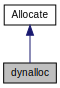
\includegraphics[width=133pt]{classdynalloc__inherit__graph}
\end{center}
\end{figure}


Collaboration diagram for dynalloc\+:
\nopagebreak
\begin{figure}[H]
\begin{center}
\leavevmode
\includegraphics[width=323pt]{classdynalloc__coll__graph}
\end{center}
\end{figure}
\subsection*{Public Member Functions}
\begin{DoxyCompactItemize}
\item 
\hyperlink{classdynalloc_ad5aa0343bab70d1f51e05953d890e8d2}{dynalloc} (\hyperlink{classraft_1_1map}{raft\+::map} \&map, volatile bool \&\hyperlink{class_allocate_a4d10076b88ab1297c89b8a05e117b510}{exit\+\_\+alloc})
\item 
virtual void \hyperlink{classdynalloc_a2a52b86ec09bd6dd52e49062137b2e37}{run} ()
\end{DoxyCompactItemize}
\subsection*{Additional Inherited Members}


\subsection{Detailed Description}


Definition at line 29 of file dynalloc.\+hpp.



\subsection{Constructor \& Destructor Documentation}
\hypertarget{classdynalloc_ad5aa0343bab70d1f51e05953d890e8d2}{}\label{classdynalloc_ad5aa0343bab70d1f51e05953d890e8d2} 
\index{dynalloc@{dynalloc}!dynalloc@{dynalloc}}
\index{dynalloc@{dynalloc}!dynalloc@{dynalloc}}
\subsubsection{\texorpdfstring{dynalloc()}{dynalloc()}}
{\footnotesize\ttfamily dynalloc\+::dynalloc (\begin{DoxyParamCaption}\item[{\hyperlink{classraft_1_1map}{raft\+::map} \&}]{map,  }\item[{volatile bool \&}]{exit\+\_\+alloc }\end{DoxyParamCaption})}

\hyperlink{dynalloc_8cpp_source}{dynalloc.\+cpp} -\/ \begin{DoxyAuthor}{Author}
\+: Jonathan Beard 
\end{DoxyAuthor}
\begin{DoxyVersion}{Version}
\+: Mon Oct 13 16\+:36\+:18 2014
\end{DoxyVersion}
Copyright 2014 Jonathan Beard

Licensed under the Apache License, Version 2.\+0 (the \char`\"{}\+License\char`\"{}); you may not use this file except in compliance with the License. You may obtain a copy of the License at\+:

\href{http://www.apache.org/licenses/LICENSE-2.0}{\tt http\+://www.\+apache.\+org/licenses/\+L\+I\+C\+E\+N\+S\+E-\/2.\+0}

Unless required by applicable law or agreed to in writing, software distributed under the License is distributed on an \char`\"{}\+A\+S I\+S\char`\"{} B\+A\+S\+IS, W\+I\+T\+H\+O\+UT W\+A\+R\+R\+A\+N\+T\+I\+ES OR C\+O\+N\+D\+I\+T\+I\+O\+NS OF A\+NY K\+I\+ND, either express or implied. See the License for the specific language governing permissions and limitations under the License. 

Definition at line 35 of file dynalloc.\+cpp.


\begin{DoxyCode}
36                                                 :
37                         \hyperlink{class_allocate_ab2b82e7fab9d0fccb9702effec93917b}{Allocate}( map, \hyperlink{class_allocate_a4d10076b88ab1297c89b8a05e117b510}{exit\_alloc} )
38 \{
39 \}
\end{DoxyCode}


\subsection{Member Function Documentation}
\hypertarget{classdynalloc_a2a52b86ec09bd6dd52e49062137b2e37}{}\label{classdynalloc_a2a52b86ec09bd6dd52e49062137b2e37} 
\index{dynalloc@{dynalloc}!run@{run}}
\index{run@{run}!dynalloc@{dynalloc}}
\subsubsection{\texorpdfstring{run()}{run()}}
{\footnotesize\ttfamily void dynalloc\+::run (\begin{DoxyParamCaption}{ }\end{DoxyParamCaption})\hspace{0.3cm}{\ttfamily [virtual]}}

run -\/ call to initiate schedule, in the current instantiation this is called by the scheduler. same alloc for all, inherit from base alloc

acquire source kernels

make this a fixed quantity right now, if size $>$ .75\% at montor interval three times or more then increase size.

T\+O\+DO, the values might wrap if no monitoring on

get initializer function

start monitor loop

monitor fifo\textquotesingle{}s 

Implements \hyperlink{class_allocate_a44f9b51c382fec159233609e21b9d272}{Allocate}.



Definition at line 65 of file dynalloc.\+cpp.



References Graph\+Tools\+::\+B\+F\+S(), Allocate\+::exit\+\_\+alloc, F\+I\+F\+O\+::get\+\_\+frac\+\_\+write\+\_\+blocked(), Port\+Info\+::get\+F\+I\+F\+O(), Allocate\+::set\+Ready(), and Allocate\+::source\+\_\+kernels.


\begin{DoxyCode}
66 \{
67    \textcolor{keyword}{auto} alloc\_func = [&]( \hyperlink{struct_port_info}{PortInfo} &a, \hyperlink{struct_port_info}{PortInfo} &b, \textcolor{keywordtype}{void} *data )
68    \{\textcolor{comment}{}
69 \textcolor{comment}{      /** same alloc for all, inherit from base alloc **/}
70       (\textcolor{keyword}{this})->allocate( a, b, data );
71    \};
72 \textcolor{comment}{}
73 \textcolor{comment}{   /** acquire source kernels **/}
74    \textcolor{keyword}{auto} &container( (\textcolor{keyword}{this})->\hyperlink{class_allocate_a93e612d7ea7eb686fc88b5dee7a1407b}{source\_kernels}.acquire() );
75    \hyperlink{class_graph_tools_ade51007699cbd681c1a37946609c46ee}{GraphTools::BFS}( container, alloc\_func );
76    (\textcolor{keyword}{this})->\hyperlink{class_allocate_a93e612d7ea7eb686fc88b5dee7a1407b}{source\_kernels}.release();
77    (\textcolor{keyword}{this})->\hyperlink{class_allocate_a4cf36bb704e43f5736a0e736d9e1a81b}{setReady}();
78    std::map< std::size\_t, int > size\_map;
79 \textcolor{comment}{}
80 \textcolor{comment}{   /**}
81 \textcolor{comment}{    * make this a fixed quantity right now, if size > .75% at}
82 \textcolor{comment}{    * montor interval three times or more then increase size.}
83 \textcolor{comment}{    */}
84 
85    \textcolor{keyword}{auto} mon\_func = [&]( \hyperlink{struct_port_info}{PortInfo} &a, \hyperlink{struct_port_info}{PortInfo} &b, \textcolor{keywordtype}{void} *data ) -> \textcolor{keywordtype}{void}
86    \{
87       (void) data;
88 
89       \textcolor{keyword}{const} \textcolor{keyword}{auto} hash\_val( dynalloc::hash( a, b ) );\textcolor{comment}{}
90 \textcolor{comment}{      /** TODO, the values might wrap if no monitoring on **/}
91       \textcolor{keyword}{const} \textcolor{keyword}{auto} realized\_ratio( a.\hyperlink{struct_port_info_a483d162fbe356e07381c6c5cfccb4f48}{getFIFO}()->\hyperlink{class_f_i_f_o_a4d44784c43a4026508e85982eb3174c7}{get\_frac\_write\_blocked}() );
92       \textcolor{keyword}{const} \textcolor{keyword}{auto} ratio( 0.8 );
93       \textcolor{keywordflow}{if}( realized\_ratio >= ratio )
94       \{
95          \textcolor{keyword}{const} \textcolor{keyword}{auto} curr\_count( size\_map[ hash\_val ]++ );
96          \textcolor{keywordflow}{if}( curr\_count  > 2 )
97          \{\textcolor{comment}{}
98 \textcolor{comment}{            /** get initializer function **/}
99             \textcolor{keyword}{auto} * \textcolor{keyword}{const} buff\_ptr( a.\hyperlink{struct_port_info_a483d162fbe356e07381c6c5cfccb4f48}{getFIFO}() );
100             \textcolor{keyword}{const} \textcolor{keyword}{auto} cap( buff\_ptr->capacity() );
101             buff\_ptr->resize( cap * 2, ALLOC\_ALIGN\_WIDTH, \hyperlink{class_allocate_a4d10076b88ab1297c89b8a05e117b510}{exit\_alloc} );
102             size\_map[ hash\_val ] = 0;
103          \}
104       \}
105       \textcolor{keywordflow}{return};
106    \};\textcolor{comment}{}
107 \textcolor{comment}{   /** start monitor loop **/}
108    \textcolor{keywordflow}{while}( ! \hyperlink{class_allocate_a4d10076b88ab1297c89b8a05e117b510}{exit\_alloc} )
109    \{\textcolor{comment}{}
110 \textcolor{comment}{      /** monitor fifo's **/}
111       std::chrono::microseconds dura( 3000 );
112       std::this\_thread::sleep\_for( dura );
113 
114       \textcolor{keyword}{auto} &container( (\textcolor{keyword}{this})->\hyperlink{class_allocate_a93e612d7ea7eb686fc88b5dee7a1407b}{source\_kernels}.acquire() );
115       \hyperlink{class_graph_tools_ade51007699cbd681c1a37946609c46ee}{GraphTools::BFS}( container, mon\_func );
116       (\textcolor{keyword}{this})->\hyperlink{class_allocate_a93e612d7ea7eb686fc88b5dee7a1407b}{source\_kernels}.release();
117 
118    \}
119    \textcolor{keywordflow}{return};
120 \}
\end{DoxyCode}
Here is the call graph for this function\+:
\nopagebreak
\begin{figure}[H]
\begin{center}
\leavevmode
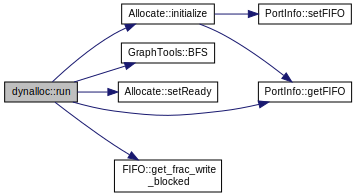
\includegraphics[width=296pt]{classdynalloc_a2a52b86ec09bd6dd52e49062137b2e37_cgraph}
\end{center}
\end{figure}


The documentation for this class was generated from the following files\+:\begin{DoxyCompactItemize}
\item 
dynalloc.\+hpp\item 
dynalloc.\+cpp\end{DoxyCompactItemize}

\hypertarget{class_f_i_f_o}{}\section{F\+I\+FO Class Reference}
\label{class_f_i_f_o}\index{F\+I\+FO@{F\+I\+FO}}
\subsection*{Public Member Functions}
\begin{DoxyCompactItemize}
\item 
\hyperlink{class_f_i_f_o_a200f4cf6db6b1994331ee4e0b2a594b1}{F\+I\+FO} ()=default
\item 
virtual \hyperlink{class_f_i_f_o_a75da1c02fbe46eb47f948f37d063dabf}{$\sim$\+F\+I\+FO} ()=default
\item 
virtual std\+::size\+\_\+t \hyperlink{class_f_i_f_o_ae80b8555fc249168560c67cd0a13e574}{size} ()=0
\item 
virtual std\+::size\+\_\+t \hyperlink{class_f_i_f_o_ac34aa9afd24e536aad0a9553863b6fe6}{space\+\_\+avail} ()=0
\item 
virtual std\+::size\+\_\+t \hyperlink{class_f_i_f_o_a64565d7156f6796ff14c3033387043b1}{capacity} ()=0
\item 
{\footnotesize template$<$class T , typename std\+::enable\+\_\+if$<$ inline\+\_\+nonclass\+\_\+alloc$<$ T $>$\+::value $>$\+::type $\ast$  = nullptr$>$ }\\T \& \hyperlink{class_f_i_f_o_a43ad12d67e3611fafae4d6ed862c60b9}{allocate} ()
\item 
{\footnotesize template$<$class T , class ... Args, typename std\+::enable\+\_\+if$<$ inline\+\_\+class\+\_\+alloc$<$ T $>$\+::value $>$\+::type $\ast$  = nullptr$>$ }\\T \& \hyperlink{class_f_i_f_o_af3ebfa2420677b5225794a361aa8dccc}{allocate} (Args \&\&... params)
\item 
{\footnotesize template$<$class T , class ... Args, typename std\+::enable\+\_\+if$<$ ext\+\_\+alloc$<$ T $>$\+::value $>$\+::type $\ast$  = nullptr$>$ }\\T \& \hyperlink{class_f_i_f_o_af3ebfa2420677b5225794a361aa8dccc}{allocate} (Args \&\&... params)
\item 
virtual void \hyperlink{class_f_i_f_o_af37b9a289093791f4bb9e4ef4e4e271a}{deallocate} ()=0
\item 
{\footnotesize template$<$class T , typename std\+::enable\+\_\+if$<$ inline\+\_\+nonclass\+\_\+alloc$<$ T $>$\+::value $>$\+::type $\ast$  = nullptr$>$ }\\auto \hyperlink{class_f_i_f_o_a9033768546db45b5f06103d32fec4b65}{allocate\+\_\+s} () -\/$>$ autorelease$<$ T, allocatetype $>$
\item 
{\footnotesize template$<$class T , class ... Args, typename std\+::enable\+\_\+if$<$ inline\+\_\+class\+\_\+alloc$<$ T $>$\+::value $>$\+::type $\ast$  = nullptr$>$ }\\auto \hyperlink{class_f_i_f_o_aa5f5334a93f8a014eb19d488898a2e39}{allocate\+\_\+s} (Args \&\&... params) -\/$>$ autorelease$<$ T, allocatetype $>$
\item 
{\footnotesize template$<$class T $>$ }\\auto \hyperlink{class_f_i_f_o_a8b93da58a3fd6ecd844827c4fcbd2473}{allocate\+\_\+range} (const std\+::size\+\_\+t n) -\/$>$ std\+::vector$<$ std\+::reference\+\_\+wrapper$<$ T $>$ $>$
\item 
virtual void \hyperlink{class_f_i_f_o_a0bb564ddace3951ed7754a285b438ba4}{send} (const raft\+::signal=raft\+::none)=0
\item 
virtual void \hyperlink{class_f_i_f_o_ac0be4de6db251e1a2e6dcc97a5d4a584}{send\+\_\+range} (const raft\+::signal=raft\+::none)=0
\item 
{\footnotesize template$<$class T $>$ }\\void \hyperlink{class_f_i_f_o_a381974271d6c818473edd23c355f0d36}{push} (const T \&item, const raft\+::signal signal=raft\+::none)
\item 
{\footnotesize template$<$class T $>$ }\\void \hyperlink{class_f_i_f_o_ad1237dfa071d0ca2002bd5aa0ce6d203}{push} (const T \&\&item, const raft\+::signal signal=raft\+::none)
\item 
{\footnotesize template$<$class iterator\+\_\+type $>$ }\\void \hyperlink{class_f_i_f_o_a922b94b854cc9e3ee37fbd447982f663}{insert} (iterator\+\_\+type begin, iterator\+\_\+type end, const raft\+::signal signal=raft\+::none)
\item 
{\footnotesize template$<$class T $>$ }\\void \hyperlink{class_f_i_f_o_a0607b6c931ed1fab618e637af617dd15}{pop} (T \&item, raft\+::signal $\ast$signal=nullptr)
\item 
\hypertarget{class_f_i_f_o_ad0ae6389ad4f59a38eb859f1b7d5db1f}{}\label{class_f_i_f_o_ad0ae6389ad4f59a38eb859f1b7d5db1f} 
{\footnotesize template$<$class T $>$ }\\auto {\bfseries pop\+\_\+s} () -\/$>$ autorelease$<$ T, poptype $>$
\item 
{\footnotesize template$<$class T $>$ }\\void \hyperlink{class_f_i_f_o_a23be63e817ff487d32013064e752f02f}{pop\+\_\+range} (pop\+\_\+range\+\_\+t$<$ T $>$ \&items, const std\+::size\+\_\+t n\+\_\+items)
\item 
{\footnotesize template$<$class T , typename std\+::enable\+\_\+if$<$ inline\+\_\+alloc$<$ T $>$\+::value $>$\+::type $\ast$  = nullptr$>$ }\\T \& \hyperlink{class_f_i_f_o_a8721e94d35fdfb20294ae8478d0baae5}{peek} (raft\+::signal $\ast$signal=nullptr)
\item 
\hypertarget{class_f_i_f_o_a8721e94d35fdfb20294ae8478d0baae5}{}\label{class_f_i_f_o_a8721e94d35fdfb20294ae8478d0baae5} 
{\footnotesize template$<$class T , typename std\+::enable\+\_\+if$<$ ext\+\_\+alloc$<$ T $>$\+::value $>$\+::type $\ast$  = nullptr$>$ }\\T \& {\bfseries peek} (raft\+::signal $\ast$signal=nullptr)
\item 
{\footnotesize template$<$class T , typename std\+::enable\+\_\+if$<$ inline\+\_\+alloc$<$ T $>$\+::value $>$\+::type $\ast$  = nullptr$>$ }\\auto \hyperlink{class_f_i_f_o_ada716e83c59345f73295d3b6f720681f}{peek\+\_\+range} (const std\+::size\+\_\+t n) -\/$>$ autorelease$<$ T, peekrange $>$
\item 
{\footnotesize template$<$class T , typename std\+::enable\+\_\+if$<$ ext\+\_\+alloc$<$ T $>$\+::value $>$\+::type $\ast$  = nullptr$>$ }\\auto \hyperlink{class_f_i_f_o_ada716e83c59345f73295d3b6f720681f}{peek\+\_\+range} (const std\+::size\+\_\+t n) -\/$>$ autorelease$<$ T, peekrange $>$
\item 
virtual void \hyperlink{class_f_i_f_o_aa0cbb6c4a5b8783af38c6deb1a6f651e}{unpeek} ()=0
\item 
void \hyperlink{class_f_i_f_o_abac84fe2d1e4b83df8571a97abf9a713}{recycle} (const std\+::size\+\_\+t range=1)
\item 
virtual void \hyperlink{class_f_i_f_o_aa372ba61179c80ce8355aadbdbbad844}{get\+\_\+zero\+\_\+read\+\_\+stats} (\hyperlink{struct_blocked}{Blocked} \&copy)
\item 
virtual void \hyperlink{class_f_i_f_o_a6dd419cc4b99bd13f6b018145844bdd2}{get\+\_\+zero\+\_\+write\+\_\+stats} (\hyperlink{struct_blocked}{Blocked} \&copy)
\item 
virtual void \hyperlink{class_f_i_f_o_a27264d14b86811604a54e0d30aa22c33}{resize} (const std\+::size\+\_\+t n\+\_\+items, const std\+::size\+\_\+t align, volatile bool \&exit\+\_\+alloc)=0
\item 
virtual float \hyperlink{class_f_i_f_o_a4d44784c43a4026508e85982eb3174c7}{get\+\_\+frac\+\_\+write\+\_\+blocked} ()=0
\item 
virtual void \hyperlink{class_f_i_f_o_af65e8231c0d1a7cdf250f2ce57f3723f}{invalidate} ()=0
\item 
virtual bool \hyperlink{class_f_i_f_o_a01bc45169bff5253496dc6bf6f902f89}{is\+\_\+invalid} ()=0
\end{DoxyCompactItemize}
\subsection*{Protected Member Functions}
\begin{DoxyCompactItemize}
\item 
virtual void \hyperlink{class_f_i_f_o_a6d7f0cf28c0eba5eaa12c347734dbdf2}{set\+Ptr\+Map} (ptr\+\_\+map\+\_\+t $\ast$const in)
\item 
virtual void \hyperlink{class_f_i_f_o_a866988c11d53fae77d6ac6f0b56aae56}{set\+Ptr\+Set} (ptr\+\_\+set\+\_\+t $\ast$const out)
\item 
virtual void \hyperlink{class_f_i_f_o_abccc27a45f6590bb8529513c411b0b5a}{set\+In\+Peek\+Set} (ptr\+\_\+set\+\_\+t $\ast$const peekset)
\item 
virtual void \hyperlink{class_f_i_f_o_aaf19d035ab4e130dbcd78c576cdf0dae}{set\+Out\+Peek\+Set} (ptr\+\_\+set\+\_\+t $\ast$const peekset)
\item 
virtual void \hyperlink{class_f_i_f_o_aa9c1f679b4e2585047af2c09a2518209}{set\+\_\+src\+\_\+kernel} (\hyperlink{classraft_1_1kernel}{raft\+::kernel} $\ast$const k)=0
\item 
virtual void \hyperlink{class_f_i_f_o_a11422695c75c05ad2c60e662553f2667}{set\+\_\+dst\+\_\+kernel} (\hyperlink{classraft_1_1kernel}{raft\+::kernel} $\ast$const k)=0
\item 
virtual raft\+::signal \hyperlink{class_f_i_f_o_a36a7519af834c969d49f3d9ae7080af9}{signal\+\_\+peek} ()=0
\item 
virtual void \hyperlink{class_f_i_f_o_ad6b606d47361489007490e0e0b4e2aa1}{signal\+\_\+pop} ()=0
\item 
virtual void \hyperlink{class_f_i_f_o_ae7e91c74078cd52cdfc6f3609b83c8eb}{inline\+\_\+signal\+\_\+send} (const raft\+::signal sig)=0
\item 
virtual void \hyperlink{class_f_i_f_o_a60068cb00b13626e41d4b11099354ae3}{local\+\_\+allocate} (void $\ast$$\ast$ptr)=0
\item 
virtual void \hyperlink{class_f_i_f_o_a4acc34ebbad9df32f54ae8c618ffa0c0}{local\+\_\+allocate\+\_\+n} (void $\ast$ptr, const std\+::size\+\_\+t n)=0
\item 
virtual void \hyperlink{class_f_i_f_o_a4ef48ce2cb02e8bd5d381bb65687e6cb}{local\+\_\+push} (void $\ast$ptr, const raft\+::signal \&signal)=0
\item 
virtual void \hyperlink{class_f_i_f_o_ab3e42eddd74c0c5ce4a640c0cc022245}{local\+\_\+insert} (void $\ast$ptr\+\_\+begin, void $\ast$ptr\+\_\+end, const raft\+::signal \&signal, const std\+::size\+\_\+t iterator\+\_\+type)=0
\item 
virtual void \hyperlink{class_f_i_f_o_ad7ca430a795bbf0904c041dcdfd836a4}{local\+\_\+pop} (void $\ast$ptr, raft\+::signal $\ast$signal)=0
\item 
virtual void \hyperlink{class_f_i_f_o_ab57165cd95da922e5432577893ab2e28}{local\+\_\+pop\+\_\+range} (void $\ast$ptr\+\_\+data, const std\+::size\+\_\+t n\+\_\+items)=0
\item 
virtual void \hyperlink{class_f_i_f_o_afc960790e2803da85fa24e64c61c38b5}{local\+\_\+peek} (void $\ast$$\ast$ptr, raft\+::signal $\ast$signal)=0
\item 
virtual void \hyperlink{class_f_i_f_o_a8056adb06fadf2b7aae4d9858795be45}{local\+\_\+peek\+\_\+range} (void $\ast$$\ast$ptr, void $\ast$$\ast$sig, const std\+::size\+\_\+t n\+\_\+items, std\+::size\+\_\+t \&curr\+\_\+pointer\+\_\+loc)=0
\item 
virtual void \hyperlink{class_f_i_f_o_a72ba5eed0ad96d6f65414f1070a2ac37}{local\+\_\+recycle} (std\+::size\+\_\+t range)=0
\end{DoxyCompactItemize}
\subsection*{Friends}
\begin{DoxyCompactItemize}
\item 
class \hyperlink{class_f_i_f_o_aae5808dc2e987bf17ef42196457a654d}{Schedule}
\item 
\hypertarget{class_f_i_f_o_a64fd97b135f77d4b136e8fff9a1c1ae1}{}\label{class_f_i_f_o_a64fd97b135f77d4b136e8fff9a1c1ae1} 
class {\bfseries Allocate}
\end{DoxyCompactItemize}


\subsection{Detailed Description}


Definition at line 51 of file fifo.\+hpp.



\subsection{Constructor \& Destructor Documentation}
\hypertarget{class_f_i_f_o_a200f4cf6db6b1994331ee4e0b2a594b1}{}\label{class_f_i_f_o_a200f4cf6db6b1994331ee4e0b2a594b1} 
\index{F\+I\+FO@{F\+I\+FO}!F\+I\+FO@{F\+I\+FO}}
\index{F\+I\+FO@{F\+I\+FO}!F\+I\+FO@{F\+I\+FO}}
\subsubsection{\texorpdfstring{F\+I\+F\+O()}{FIFO()}}
{\footnotesize\ttfamily F\+I\+F\+O\+::\+F\+I\+FO (\begin{DoxyParamCaption}{ }\end{DoxyParamCaption})\hspace{0.3cm}{\ttfamily [default]}}

\hyperlink{class_f_i_f_o}{F\+I\+FO} -\/ default constructor for base class for all subsequent ringbuffers. \hypertarget{class_f_i_f_o_a75da1c02fbe46eb47f948f37d063dabf}{}\label{class_f_i_f_o_a75da1c02fbe46eb47f948f37d063dabf} 
\index{F\+I\+FO@{F\+I\+FO}!````~F\+I\+FO@{$\sim$\+F\+I\+FO}}
\index{````~F\+I\+FO@{$\sim$\+F\+I\+FO}!F\+I\+FO@{F\+I\+FO}}
\subsubsection{\texorpdfstring{$\sim$\+F\+I\+F\+O()}{~FIFO()}}
{\footnotesize\ttfamily virtual F\+I\+F\+O\+::$\sim$\+F\+I\+FO (\begin{DoxyParamCaption}{ }\end{DoxyParamCaption})\hspace{0.3cm}{\ttfamily [virtual]}, {\ttfamily [default]}}

$\sim$\+F\+I\+FO -\/ default destructor 

\subsection{Member Function Documentation}
\hypertarget{class_f_i_f_o_a43ad12d67e3611fafae4d6ed862c60b9}{}\label{class_f_i_f_o_a43ad12d67e3611fafae4d6ed862c60b9} 
\index{F\+I\+FO@{F\+I\+FO}!allocate@{allocate}}
\index{allocate@{allocate}!F\+I\+FO@{F\+I\+FO}}
\subsubsection{\texorpdfstring{allocate()}{allocate()}\hspace{0.1cm}{\footnotesize\ttfamily [1/3]}}
{\footnotesize\ttfamily template$<$class T , typename std\+::enable\+\_\+if$<$ inline\+\_\+nonclass\+\_\+alloc$<$ T $>$\+::value $>$\+::type $\ast$  = nullptr$>$ \\
T\& F\+I\+F\+O\+::allocate (\begin{DoxyParamCaption}{ }\end{DoxyParamCaption})\hspace{0.3cm}{\ttfamily [inline]}}

allocate -\/ returns a reference to a writeable member at the tail of the \hyperlink{class_f_i_f_o}{F\+I\+FO}. You must have a subsequent call to send in order to release this object to the \hyperlink{class_f_i_f_o}{F\+I\+FO} once it is written. If the user needs to de-\/allocate the memory without using it, they can call the deallocate function. \begin{DoxyReturn}{Returns}
T\& 
\end{DoxyReturn}
call blocks till an element is available 

Definition at line 101 of file fifo.\+hpp.


\begin{DoxyCode}
102    \{
103       \textcolor{keywordtype}{void} *ptr( \textcolor{keyword}{nullptr} );\textcolor{comment}{}
104 \textcolor{comment}{      /** call blocks till an element is available **/}
105       \hyperlink{class_f_i_f_o_a60068cb00b13626e41d4b11099354ae3}{local\_allocate}( &ptr );
106       \textcolor{keywordflow}{return}( *( reinterpret\_cast< T* >( ptr ) ) );
107    \}
\end{DoxyCode}
\hypertarget{class_f_i_f_o_af3ebfa2420677b5225794a361aa8dccc}{}\label{class_f_i_f_o_af3ebfa2420677b5225794a361aa8dccc} 
\index{F\+I\+FO@{F\+I\+FO}!allocate@{allocate}}
\index{allocate@{allocate}!F\+I\+FO@{F\+I\+FO}}
\subsubsection{\texorpdfstring{allocate()}{allocate()}\hspace{0.1cm}{\footnotesize\ttfamily [2/3]}}
{\footnotesize\ttfamily template$<$class T , class ... Args, typename std\+::enable\+\_\+if$<$ inline\+\_\+class\+\_\+alloc$<$ T $>$\+::value $>$\+::type $\ast$  = nullptr$>$ \\
T\& F\+I\+F\+O\+::allocate (\begin{DoxyParamCaption}\item[{Args \&\&...}]{params }\end{DoxyParamCaption})\hspace{0.3cm}{\ttfamily [inline]}}

call blocks till an element is available 

Definition at line 115 of file fifo.\+hpp.


\begin{DoxyCode}
116    \{
117       \textcolor{keywordtype}{void} *ptr( \textcolor{keyword}{nullptr} );\textcolor{comment}{}
118 \textcolor{comment}{      /** call blocks till an element is available **/}
119       \hyperlink{class_f_i_f_o_a60068cb00b13626e41d4b11099354ae3}{local\_allocate}( &ptr );
120       T * temp( \textcolor{keyword}{new} (ptr) T( std::forward< Args >( params )... ) );
121       UNUSED( temp );
122       \textcolor{keywordflow}{return}( *( reinterpret\_cast< T* >( ptr ) ) );
123    \}
\end{DoxyCode}
\hypertarget{class_f_i_f_o_af3ebfa2420677b5225794a361aa8dccc}{}\label{class_f_i_f_o_af3ebfa2420677b5225794a361aa8dccc} 
\index{F\+I\+FO@{F\+I\+FO}!allocate@{allocate}}
\index{allocate@{allocate}!F\+I\+FO@{F\+I\+FO}}
\subsubsection{\texorpdfstring{allocate()}{allocate()}\hspace{0.1cm}{\footnotesize\ttfamily [3/3]}}
{\footnotesize\ttfamily template$<$class T , class ... Args, typename std\+::enable\+\_\+if$<$ ext\+\_\+alloc$<$ T $>$\+::value $>$\+::type $\ast$  = nullptr$>$ \\
T\& F\+I\+F\+O\+::allocate (\begin{DoxyParamCaption}\item[{Args \&\&...}]{params }\end{DoxyParamCaption})\hspace{0.3cm}{\ttfamily [inline]}}

call blocks till an element is available 

Definition at line 129 of file fifo.\+hpp.


\begin{DoxyCode}
130    \{
131       T **ptr( \textcolor{keyword}{nullptr} );\textcolor{comment}{}
132 \textcolor{comment}{      /** call blocks till an element is available **/}
133       \hyperlink{class_f_i_f_o_a60068cb00b13626e41d4b11099354ae3}{local\_allocate}( (\textcolor{keywordtype}{void}**) &ptr );
134       *ptr = \textcolor{keyword}{new} T( std::forward< Args >( params )... );
135       \textcolor{keywordflow}{return}( **ptr );
136    \}
\end{DoxyCode}
\hypertarget{class_f_i_f_o_a8b93da58a3fd6ecd844827c4fcbd2473}{}\label{class_f_i_f_o_a8b93da58a3fd6ecd844827c4fcbd2473} 
\index{F\+I\+FO@{F\+I\+FO}!allocate\+\_\+range@{allocate\+\_\+range}}
\index{allocate\+\_\+range@{allocate\+\_\+range}!F\+I\+FO@{F\+I\+FO}}
\subsubsection{\texorpdfstring{allocate\+\_\+range()}{allocate\_range()}}
{\footnotesize\ttfamily template$<$class T $>$ \\
auto F\+I\+F\+O\+::allocate\+\_\+range (\begin{DoxyParamCaption}\item[{const std\+::size\+\_\+t}]{n }\end{DoxyParamCaption}) -\/$>$ std\+::vector$<$ std\+::reference\+\_\+wrapper$<$ T $>$ $>$
   \hspace{0.3cm}{\ttfamily [inline]}}

T\+O\+DO, fix allocate\+\_\+range to double buffer properly if not enough mem available allocate\+\_\+range -\/ returns a std\+::vector of references to n items on the queue. If for some reason the capacity of the queue is less than n or some other unspecified error occurs then the number allocated is returned in n\+\_\+ret. To release items to the queue, use push\+\_\+range as opposed to the standard push. 
\begin{DoxyParams}{Parameters}
{\em n} & -\/ const std\+::size\+\_\+t, \# items to allocate \\
\hline
\end{DoxyParams}
\begin{DoxyReturn}{Returns}
std\+::vector$<$ std\+::reference\+\_\+wrapper$<$ T $>$ $>$ 
\end{DoxyReturn}
compiler should optimize this copy, if not then it\textquotesingle{}ll be a copy of referneces not full objects 

Definition at line 207 of file fifo.\+hpp.


\begin{DoxyCode}
209    \{
210       std::vector< std::reference\_wrapper< T > > output;
211       \textcolor{keywordtype}{void} *ptr( (\textcolor{keywordtype}{void}*) &output );
212       \hyperlink{class_f_i_f_o_a4acc34ebbad9df32f54ae8c618ffa0c0}{local\_allocate\_n}( ptr, n );\textcolor{comment}{}
213 \textcolor{comment}{      /** compiler should optimize this copy, if not then it'll be a copy of referneces not full objects *
      */}
214       \textcolor{keywordflow}{return}( std::forward<
215          std::vector< 
216             std::reference\_wrapper< T > > >( output ) );
217    \}
\end{DoxyCode}
\hypertarget{class_f_i_f_o_a9033768546db45b5f06103d32fec4b65}{}\label{class_f_i_f_o_a9033768546db45b5f06103d32fec4b65} 
\index{F\+I\+FO@{F\+I\+FO}!allocate\+\_\+s@{allocate\+\_\+s}}
\index{allocate\+\_\+s@{allocate\+\_\+s}!F\+I\+FO@{F\+I\+FO}}
\subsubsection{\texorpdfstring{allocate\+\_\+s()}{allocate\_s()}\hspace{0.1cm}{\footnotesize\ttfamily [1/2]}}
{\footnotesize\ttfamily template$<$class T , typename std\+::enable\+\_\+if$<$ inline\+\_\+nonclass\+\_\+alloc$<$ T $>$\+::value $>$\+::type $\ast$  = nullptr$>$ \\
auto F\+I\+F\+O\+::allocate\+\_\+s (\begin{DoxyParamCaption}{ }\end{DoxyParamCaption}) -\/$>$ autorelease$<$ T, allocatetype $>$
   \hspace{0.3cm}{\ttfamily [inline]}}

allocate\+\_\+s -\/ \char`\"{}auto-\/release\char`\"{} version of allocate, where the action of pushing the memory allocated to the consumer is handled by the returned object exiting the calling stack frame. There are two functions here, one that uses the objec constructor type. This one is for plain old data types. \begin{DoxyReturn}{Returns}
autorelease$<$ T, allocatetype $>$ 
\end{DoxyReturn}


Definition at line 157 of file fifo.\+hpp.


\begin{DoxyCode}
158    \{
159       \textcolor{keywordtype}{void} *ptr( \textcolor{keyword}{nullptr} );
160       \hyperlink{class_f_i_f_o_a60068cb00b13626e41d4b11099354ae3}{local\_allocate}( &ptr );
161       \textcolor{keywordflow}{return}( autorelease< T, allocatetype >( 
162          reinterpret\_cast< T* >( ptr ), (*\textcolor{keyword}{this}) ) );
163    \}
\end{DoxyCode}
\hypertarget{class_f_i_f_o_aa5f5334a93f8a014eb19d488898a2e39}{}\label{class_f_i_f_o_aa5f5334a93f8a014eb19d488898a2e39} 
\index{F\+I\+FO@{F\+I\+FO}!allocate\+\_\+s@{allocate\+\_\+s}}
\index{allocate\+\_\+s@{allocate\+\_\+s}!F\+I\+FO@{F\+I\+FO}}
\subsubsection{\texorpdfstring{allocate\+\_\+s()}{allocate\_s()}\hspace{0.1cm}{\footnotesize\ttfamily [2/2]}}
{\footnotesize\ttfamily template$<$class T , class ... Args, typename std\+::enable\+\_\+if$<$ inline\+\_\+class\+\_\+alloc$<$ T $>$\+::value $>$\+::type $\ast$  = nullptr$>$ \\
auto F\+I\+F\+O\+::allocate\+\_\+s (\begin{DoxyParamCaption}\item[{Args \&\&...}]{params }\end{DoxyParamCaption}) -\/$>$ autorelease$<$ T, allocatetype $>$
   \hspace{0.3cm}{\ttfamily [inline]}}

allocate\+\_\+s -\/ \char`\"{}auto-\/release\char`\"{} version of allocate, where the action of pushing the memory allocated to the consumer is handled by the returned object exiting the calling stack frame. There are two functions here, one that uses the objec constructor type. This one is for object types. \begin{DoxyReturn}{Returns}
autorelease$<$ T, allocatetype $>$ 
\end{DoxyReturn}
call blocks till an element is available 

Definition at line 178 of file fifo.\+hpp.


\begin{DoxyCode}
179    \{
180       \textcolor{keywordtype}{void} *ptr( \textcolor{keyword}{nullptr} );\textcolor{comment}{}
181 \textcolor{comment}{      /** call blocks till an element is available **/}
182       \hyperlink{class_f_i_f_o_a60068cb00b13626e41d4b11099354ae3}{local\_allocate}( &ptr );
183       T * \_\_attribute\_\_((\_\_unused\_\_)) temp( 
184          new (ptr) T( std::forward< Args >( params )... ) );
185       return( autorelease< T, allocatetype >( 
186          reinterpret\_cast< T* >( ptr ), (*this) ) );
187    \}
\end{DoxyCode}
\hypertarget{class_f_i_f_o_a64565d7156f6796ff14c3033387043b1}{}\label{class_f_i_f_o_a64565d7156f6796ff14c3033387043b1} 
\index{F\+I\+FO@{F\+I\+FO}!capacity@{capacity}}
\index{capacity@{capacity}!F\+I\+FO@{F\+I\+FO}}
\subsubsection{\texorpdfstring{capacity()}{capacity()}}
{\footnotesize\ttfamily virtual std\+::size\+\_\+t F\+I\+F\+O\+::capacity (\begin{DoxyParamCaption}{ }\end{DoxyParamCaption})\hspace{0.3cm}{\ttfamily [pure virtual]}}

capacity -\/ returns the set maximum capacity of the \hyperlink{class_f_i_f_o}{F\+I\+FO}. \begin{DoxyReturn}{Returns}
std\+::size\+\_\+t 
\end{DoxyReturn}
\hypertarget{class_f_i_f_o_af37b9a289093791f4bb9e4ef4e4e271a}{}\label{class_f_i_f_o_af37b9a289093791f4bb9e4ef4e4e271a} 
\index{F\+I\+FO@{F\+I\+FO}!deallocate@{deallocate}}
\index{deallocate@{deallocate}!F\+I\+FO@{F\+I\+FO}}
\subsubsection{\texorpdfstring{deallocate()}{deallocate()}}
{\footnotesize\ttfamily virtual void F\+I\+F\+O\+::deallocate (\begin{DoxyParamCaption}{ }\end{DoxyParamCaption})\hspace{0.3cm}{\ttfamily [pure virtual]}}

deallocate -\/ call after allocate if memory allocated is not needed. Will deallocate all memory allocated by a previous allocate call. \hypertarget{class_f_i_f_o_a4d44784c43a4026508e85982eb3174c7}{}\label{class_f_i_f_o_a4d44784c43a4026508e85982eb3174c7} 
\index{F\+I\+FO@{F\+I\+FO}!get\+\_\+frac\+\_\+write\+\_\+blocked@{get\+\_\+frac\+\_\+write\+\_\+blocked}}
\index{get\+\_\+frac\+\_\+write\+\_\+blocked@{get\+\_\+frac\+\_\+write\+\_\+blocked}!F\+I\+FO@{F\+I\+FO}}
\subsubsection{\texorpdfstring{get\+\_\+frac\+\_\+write\+\_\+blocked()}{get\_frac\_write\_blocked()}}
{\footnotesize\ttfamily virtual float F\+I\+F\+O\+::get\+\_\+frac\+\_\+write\+\_\+blocked (\begin{DoxyParamCaption}{ }\end{DoxyParamCaption})\hspace{0.3cm}{\ttfamily [pure virtual]}}

get\+\_\+frac\+\_\+write\+\_\+blocked -\/ returns the fraction of time that this queue was blocked. This might become a private function accessible only to the dynamic allocator mechanism, but for now its a public function. \begin{DoxyReturn}{Returns}
float 
\end{DoxyReturn}


Referenced by dynalloc\+::run().

\hypertarget{class_f_i_f_o_aa372ba61179c80ce8355aadbdbbad844}{}\label{class_f_i_f_o_aa372ba61179c80ce8355aadbdbbad844} 
\index{F\+I\+FO@{F\+I\+FO}!get\+\_\+zero\+\_\+read\+\_\+stats@{get\+\_\+zero\+\_\+read\+\_\+stats}}
\index{get\+\_\+zero\+\_\+read\+\_\+stats@{get\+\_\+zero\+\_\+read\+\_\+stats}!F\+I\+FO@{F\+I\+FO}}
\subsubsection{\texorpdfstring{get\+\_\+zero\+\_\+read\+\_\+stats()}{get\_zero\_read\_stats()}}
{\footnotesize\ttfamily void F\+I\+F\+O\+::get\+\_\+zero\+\_\+read\+\_\+stats (\begin{DoxyParamCaption}\item[{\hyperlink{struct_blocked}{Blocked} \&}]{copy }\end{DoxyParamCaption})\hspace{0.3cm}{\ttfamily [virtual]}}

get\+\_\+zero\+\_\+read\+\_\+stats -\/ sets the param variable to the current blocked stats and then sets the current vars to zero. Default version here does nothing, when instrumentation is enabled then the function called actually does something. 
\begin{DoxyParams}{Parameters}
{\em copy} & -\/ \hyperlink{struct_blocked}{Blocked}\&\\
\hline
\end{DoxyParams}
\hyperlink{fifo_8cpp_source}{F\+I\+F\+O.\+cpp} -\/ \begin{DoxyAuthor}{Author}
\+: Jonathan Beard 
\end{DoxyAuthor}
\begin{DoxyVersion}{Version}
\+: Thu Sep 4 12\+:59\+:45 2014
\end{DoxyVersion}
Copyright 2014 Jonathan Beard

Licensed under the Apache License, Version 2.\+0 (the \char`\"{}\+License\char`\"{}); you may not use this file except in compliance with the License. You may obtain a copy of the License at\+:

\href{http://www.apache.org/licenses/LICENSE-2.0}{\tt http\+://www.\+apache.\+org/licenses/\+L\+I\+C\+E\+N\+S\+E-\/2.\+0}

Unless required by applicable law or agreed to in writing, software distributed under the License is distributed on an \char`\"{}\+A\+S I\+S\char`\"{} B\+A\+S\+IS, W\+I\+T\+H\+O\+UT W\+A\+R\+R\+A\+N\+T\+I\+ES OR C\+O\+N\+D\+I\+T\+I\+O\+NS OF A\+NY K\+I\+ND, either express or implied. See the License for the specific language governing permissions and limitations under the License. default version does nothing at all 

Definition at line 24 of file fifo.\+cpp.


\begin{DoxyCode}
25 \{\textcolor{comment}{}
26 \textcolor{comment}{   /** default version does nothing at all **/}
27    UNUSED( copy ); 
28    \textcolor{keywordflow}{return};
29 \}
\end{DoxyCode}
\hypertarget{class_f_i_f_o_a6dd419cc4b99bd13f6b018145844bdd2}{}\label{class_f_i_f_o_a6dd419cc4b99bd13f6b018145844bdd2} 
\index{F\+I\+FO@{F\+I\+FO}!get\+\_\+zero\+\_\+write\+\_\+stats@{get\+\_\+zero\+\_\+write\+\_\+stats}}
\index{get\+\_\+zero\+\_\+write\+\_\+stats@{get\+\_\+zero\+\_\+write\+\_\+stats}!F\+I\+FO@{F\+I\+FO}}
\subsubsection{\texorpdfstring{get\+\_\+zero\+\_\+write\+\_\+stats()}{get\_zero\_write\_stats()}}
{\footnotesize\ttfamily void F\+I\+F\+O\+::get\+\_\+zero\+\_\+write\+\_\+stats (\begin{DoxyParamCaption}\item[{\hyperlink{struct_blocked}{Blocked} \&}]{copy }\end{DoxyParamCaption})\hspace{0.3cm}{\ttfamily [virtual]}}

get\+\_\+zero\+\_\+write\+\_\+stats -\/ sets the param variable to the current blocked stats and then sets the current vars to zero. Default version here does nothing, when instrumentation is enabled then the function, called actually does something. 
\begin{DoxyParams}{Parameters}
{\em copy} & -\/ \hyperlink{struct_blocked}{Blocked}\& \\
\hline
\end{DoxyParams}
default version does nothing at all 

Definition at line 32 of file fifo.\+cpp.


\begin{DoxyCode}
33 \{\textcolor{comment}{}
34 \textcolor{comment}{   /** default version does nothing at all **/}
35    UNUSED( copy );
36    \textcolor{keywordflow}{return};
37 \}
\end{DoxyCode}
\hypertarget{class_f_i_f_o_ae7e91c74078cd52cdfc6f3609b83c8eb}{}\label{class_f_i_f_o_ae7e91c74078cd52cdfc6f3609b83c8eb} 
\index{F\+I\+FO@{F\+I\+FO}!inline\+\_\+signal\+\_\+send@{inline\+\_\+signal\+\_\+send}}
\index{inline\+\_\+signal\+\_\+send@{inline\+\_\+signal\+\_\+send}!F\+I\+FO@{F\+I\+FO}}
\subsubsection{\texorpdfstring{inline\+\_\+signal\+\_\+send()}{inline\_signal\_send()}}
{\footnotesize\ttfamily virtual void F\+I\+F\+O\+::inline\+\_\+signal\+\_\+send (\begin{DoxyParamCaption}\item[{const raft\+::signal}]{sig }\end{DoxyParamCaption})\hspace{0.3cm}{\ttfamily [protected]}, {\ttfamily [pure virtual]}}

inline\+\_\+signal\+\_\+send -\/ pretty much exactly like it sounds, the implementations of this function must pass a signal inline with the data stream so that this signal is received immediately after the data element sent before it. 
\begin{DoxyParams}{Parameters}
{\em sig} & -\/ raft\+::signal, signal to be sent \\
\hline
\end{DoxyParams}
\hypertarget{class_f_i_f_o_a922b94b854cc9e3ee37fbd447982f663}{}\label{class_f_i_f_o_a922b94b854cc9e3ee37fbd447982f663} 
\index{F\+I\+FO@{F\+I\+FO}!insert@{insert}}
\index{insert@{insert}!F\+I\+FO@{F\+I\+FO}}
\subsubsection{\texorpdfstring{insert()}{insert()}}
{\footnotesize\ttfamily template$<$class iterator\+\_\+type $>$ \\
void F\+I\+F\+O\+::insert (\begin{DoxyParamCaption}\item[{iterator\+\_\+type}]{begin,  }\item[{iterator\+\_\+type}]{end,  }\item[{const raft\+::signal}]{signal = {\ttfamily raft\+:\+:none} }\end{DoxyParamCaption})\hspace{0.3cm}{\ttfamily [inline]}}

insert -\/ inserts the range from begin to end in the \hyperlink{class_f_i_f_o}{F\+I\+FO}, blocks until space is available. If the range is greater than the space available it\textquotesingle{}ll simply block and add items as space becomes available. There is the implicit assumption that another thread is consuming the data, so eventually there will be room. 
\begin{DoxyParams}{Parameters}
{\em begin} & -\/ iterator\+\_\+type, iterator to begin of range \\
\hline
{\em end} & -\/ iterator\+\_\+type, iterator to end of range \\
\hline
{\em signal} & -\/ raft\+::signal, default raft\+::none \\
\hline
\end{DoxyParams}


Definition at line 287 of file fifo.\+hpp.


\begin{DoxyCode}
290    \{
291       \textcolor{keywordtype}{void} *begin\_ptr( reinterpret\_cast< void* >( &begin ) );
292       \textcolor{keywordtype}{void} *end\_ptr  ( reinterpret\_cast< void* >( &end   ) );
293       \hyperlink{class_f_i_f_o_ab3e42eddd74c0c5ce4a640c0cc022245}{local\_insert}( begin\_ptr, 
294                     end\_ptr, 
295                     signal, 
296                     \textcolor{keyword}{typeid}( iterator\_type ).hash\_code() );
297       \textcolor{keywordflow}{return};
298    \}
\end{DoxyCode}
\hypertarget{class_f_i_f_o_af65e8231c0d1a7cdf250f2ce57f3723f}{}\label{class_f_i_f_o_af65e8231c0d1a7cdf250f2ce57f3723f} 
\index{F\+I\+FO@{F\+I\+FO}!invalidate@{invalidate}}
\index{invalidate@{invalidate}!F\+I\+FO@{F\+I\+FO}}
\subsubsection{\texorpdfstring{invalidate()}{invalidate()}}
{\footnotesize\ttfamily virtual void F\+I\+F\+O\+::invalidate (\begin{DoxyParamCaption}{ }\end{DoxyParamCaption})\hspace{0.3cm}{\ttfamily [pure virtual]}}

invalidate -\/ used by producer thread to label this queue as invalid. Could be for many differing reasons, however the bottom line is that once empty, this queue will receive no extra data and the receiver must do something to deal with this type of behavior if more data is requested. 

Referenced by Schedule\+::quit\+Handler().

\hypertarget{class_f_i_f_o_a01bc45169bff5253496dc6bf6f902f89}{}\label{class_f_i_f_o_a01bc45169bff5253496dc6bf6f902f89} 
\index{F\+I\+FO@{F\+I\+FO}!is\+\_\+invalid@{is\+\_\+invalid}}
\index{is\+\_\+invalid@{is\+\_\+invalid}!F\+I\+FO@{F\+I\+FO}}
\subsubsection{\texorpdfstring{is\+\_\+invalid()}{is\_invalid()}}
{\footnotesize\ttfamily virtual bool F\+I\+F\+O\+::is\+\_\+invalid (\begin{DoxyParamCaption}{ }\end{DoxyParamCaption})\hspace{0.3cm}{\ttfamily [pure virtual]}}

is\+\_\+invalid -\/ called by the consumer thread to check if this queue is in fact valid. This is typically only called if the queue is empty or if the consumer is asking for more data than is currently available. \begin{DoxyReturn}{Returns}
bool -\/ true if invalid 
\end{DoxyReturn}
\hypertarget{class_f_i_f_o_a60068cb00b13626e41d4b11099354ae3}{}\label{class_f_i_f_o_a60068cb00b13626e41d4b11099354ae3} 
\index{F\+I\+FO@{F\+I\+FO}!local\+\_\+allocate@{local\+\_\+allocate}}
\index{local\+\_\+allocate@{local\+\_\+allocate}!F\+I\+FO@{F\+I\+FO}}
\subsubsection{\texorpdfstring{local\+\_\+allocate()}{local\_allocate()}}
{\footnotesize\ttfamily virtual void F\+I\+F\+O\+::local\+\_\+allocate (\begin{DoxyParamCaption}\item[{void $\ast$$\ast$}]{ptr }\end{DoxyParamCaption})\hspace{0.3cm}{\ttfamily [protected]}, {\ttfamily [pure virtual]}}

local\+\_\+allocate -\/ in order to get this whole thing to work with multiple \char`\"{}ports\char`\"{} contained within the same container we have to erase the type and then put it back. To do this the template function gives a void ptr mem address which is given the location to the head of the queue. Once returned the main allocate function reinterprets this as the proper object type 
\begin{DoxyParams}{Parameters}
{\em ptr} & -\/ void $\ast$$\ast$ \\
\hline
\end{DoxyParams}
\hypertarget{class_f_i_f_o_a4acc34ebbad9df32f54ae8c618ffa0c0}{}\label{class_f_i_f_o_a4acc34ebbad9df32f54ae8c618ffa0c0} 
\index{F\+I\+FO@{F\+I\+FO}!local\+\_\+allocate\+\_\+n@{local\+\_\+allocate\+\_\+n}}
\index{local\+\_\+allocate\+\_\+n@{local\+\_\+allocate\+\_\+n}!F\+I\+FO@{F\+I\+FO}}
\subsubsection{\texorpdfstring{local\+\_\+allocate\+\_\+n()}{local\_allocate\_n()}}
{\footnotesize\ttfamily virtual void F\+I\+F\+O\+::local\+\_\+allocate\+\_\+n (\begin{DoxyParamCaption}\item[{void $\ast$}]{ptr,  }\item[{const std\+::size\+\_\+t}]{n }\end{DoxyParamCaption})\hspace{0.3cm}{\ttfamily [protected]}, {\ttfamily [pure virtual]}}

local\+\_\+allocate\+\_\+n -\/ copies std\+::ref\textquotesingle{}s to the data structure passed in by ptr. 
\begin{DoxyParams}{Parameters}
{\em -\/} & ptr, void$\ast$ dereferenced std\+::vector \\
\hline
{\em -\/} & n, const std\+::size\+\_\+t \\
\hline
\end{DoxyParams}
\hypertarget{class_f_i_f_o_ab3e42eddd74c0c5ce4a640c0cc022245}{}\label{class_f_i_f_o_ab3e42eddd74c0c5ce4a640c0cc022245} 
\index{F\+I\+FO@{F\+I\+FO}!local\+\_\+insert@{local\+\_\+insert}}
\index{local\+\_\+insert@{local\+\_\+insert}!F\+I\+FO@{F\+I\+FO}}
\subsubsection{\texorpdfstring{local\+\_\+insert()}{local\_insert()}}
{\footnotesize\ttfamily virtual void F\+I\+F\+O\+::local\+\_\+insert (\begin{DoxyParamCaption}\item[{void $\ast$}]{ptr\+\_\+begin,  }\item[{void $\ast$}]{ptr\+\_\+end,  }\item[{const raft\+::signal \&}]{signal,  }\item[{const std\+::size\+\_\+t}]{iterator\+\_\+type }\end{DoxyParamCaption})\hspace{0.3cm}{\ttfamily [protected]}, {\ttfamily [pure virtual]}}

local\+\_\+insert -\/ inserts a range from ptr\+\_\+begin to ptr\+\_\+end and inserts the signal at the last element inserted, the rest of the signals are set to raft\+::none. 
\begin{DoxyParams}{Parameters}
{\em ptr\+\_\+begin} & -\/ void$\ast$ \\
\hline
{\em ptr\+\_\+end} & -\/ void$\ast$ \\
\hline
{\em signal} & -\/ const raft\+::signal\& \\
\hline
\end{DoxyParams}
\hypertarget{class_f_i_f_o_afc960790e2803da85fa24e64c61c38b5}{}\label{class_f_i_f_o_afc960790e2803da85fa24e64c61c38b5} 
\index{F\+I\+FO@{F\+I\+FO}!local\+\_\+peek@{local\+\_\+peek}}
\index{local\+\_\+peek@{local\+\_\+peek}!F\+I\+FO@{F\+I\+FO}}
\subsubsection{\texorpdfstring{local\+\_\+peek()}{local\_peek()}}
{\footnotesize\ttfamily virtual void F\+I\+F\+O\+::local\+\_\+peek (\begin{DoxyParamCaption}\item[{void $\ast$$\ast$}]{ptr,  }\item[{raft\+::signal $\ast$}]{signal }\end{DoxyParamCaption})\hspace{0.3cm}{\ttfamily [protected]}, {\ttfamily [pure virtual]}}

local\+\_\+peek -\/ peeks at the head of the queue, the element may be modified but not erased. 
\begin{DoxyParams}{Parameters}
{\em ptr} & -\/ void$\ast$$\ast$ \\
\hline
{\em signal} & -\/ raft\+::signal$\ast$ \\
\hline
\end{DoxyParams}
\hypertarget{class_f_i_f_o_a8056adb06fadf2b7aae4d9858795be45}{}\label{class_f_i_f_o_a8056adb06fadf2b7aae4d9858795be45} 
\index{F\+I\+FO@{F\+I\+FO}!local\+\_\+peek\+\_\+range@{local\+\_\+peek\+\_\+range}}
\index{local\+\_\+peek\+\_\+range@{local\+\_\+peek\+\_\+range}!F\+I\+FO@{F\+I\+FO}}
\subsubsection{\texorpdfstring{local\+\_\+peek\+\_\+range()}{local\_peek\_range()}}
{\footnotesize\ttfamily virtual void F\+I\+F\+O\+::local\+\_\+peek\+\_\+range (\begin{DoxyParamCaption}\item[{void $\ast$$\ast$}]{ptr,  }\item[{void $\ast$$\ast$}]{sig,  }\item[{const std\+::size\+\_\+t}]{n\+\_\+items,  }\item[{std\+::size\+\_\+t \&}]{curr\+\_\+pointer\+\_\+loc }\end{DoxyParamCaption})\hspace{0.3cm}{\ttfamily [protected]}, {\ttfamily [pure virtual]}}

local\+\_\+peek\+\_\+range -\/ peeks at head of queue with the specified range, data may be modified but not erased. Since the queue might be non-\/contiguous then we must return the memory location of each element. 
\begin{DoxyParams}{Parameters}
{\em ptr} & -\/ void$\ast$$\ast$, pointer to pointers at which to store the pointers to items on the queue \\
\hline
{\em sig} & -\/ void$\ast$$\ast$, same as above but for signal queue \\
\hline
{\em n\+\_\+items} & -\/ const std\+::size\+\_\+t, number of items requested \\
\hline
{\em curr\+\_\+pointer\+\_\+loc} & -\/ number of items able to be returned \\
\hline
\end{DoxyParams}
\hypertarget{class_f_i_f_o_ad7ca430a795bbf0904c041dcdfd836a4}{}\label{class_f_i_f_o_ad7ca430a795bbf0904c041dcdfd836a4} 
\index{F\+I\+FO@{F\+I\+FO}!local\+\_\+pop@{local\+\_\+pop}}
\index{local\+\_\+pop@{local\+\_\+pop}!F\+I\+FO@{F\+I\+FO}}
\subsubsection{\texorpdfstring{local\+\_\+pop()}{local\_pop()}}
{\footnotesize\ttfamily virtual void F\+I\+F\+O\+::local\+\_\+pop (\begin{DoxyParamCaption}\item[{void $\ast$}]{ptr,  }\item[{raft\+::signal $\ast$}]{signal }\end{DoxyParamCaption})\hspace{0.3cm}{\ttfamily [protected]}, {\ttfamily [pure virtual]}}

local\+\_\+pop -\/ makes a copy, pops an item from the queue and stores the copy at memory located at $\ast$ptr. 
\begin{DoxyParams}{Parameters}
{\em ptr} & -\/ void$\ast$ \\
\hline
{\em signal} & -\/ raft\+::signal$\ast$ \\
\hline
\end{DoxyParams}
\hypertarget{class_f_i_f_o_ab57165cd95da922e5432577893ab2e28}{}\label{class_f_i_f_o_ab57165cd95da922e5432577893ab2e28} 
\index{F\+I\+FO@{F\+I\+FO}!local\+\_\+pop\+\_\+range@{local\+\_\+pop\+\_\+range}}
\index{local\+\_\+pop\+\_\+range@{local\+\_\+pop\+\_\+range}!F\+I\+FO@{F\+I\+FO}}
\subsubsection{\texorpdfstring{local\+\_\+pop\+\_\+range()}{local\_pop\_range()}}
{\footnotesize\ttfamily virtual void F\+I\+F\+O\+::local\+\_\+pop\+\_\+range (\begin{DoxyParamCaption}\item[{void $\ast$}]{ptr\+\_\+data,  }\item[{const std\+::size\+\_\+t}]{n\+\_\+items }\end{DoxyParamCaption})\hspace{0.3cm}{\ttfamily [protected]}, {\ttfamily [pure virtual]}}

local\+\_\+pop\+\_\+range -\/ pops a range, of n\+\_\+items and stores them to the array of T$\ast$ items pointed to by ptr\+\_\+data. 
\begin{DoxyParams}{Parameters}
{\em ptr\+\_\+data} & -\/ void$\ast$ \\
\hline
{\em n\+\_\+items} & -\/ std\+::size\+\_\+t \\
\hline
\end{DoxyParams}
\hypertarget{class_f_i_f_o_a4ef48ce2cb02e8bd5d381bb65687e6cb}{}\label{class_f_i_f_o_a4ef48ce2cb02e8bd5d381bb65687e6cb} 
\index{F\+I\+FO@{F\+I\+FO}!local\+\_\+push@{local\+\_\+push}}
\index{local\+\_\+push@{local\+\_\+push}!F\+I\+FO@{F\+I\+FO}}
\subsubsection{\texorpdfstring{local\+\_\+push()}{local\_push()}}
{\footnotesize\ttfamily virtual void F\+I\+F\+O\+::local\+\_\+push (\begin{DoxyParamCaption}\item[{void $\ast$}]{ptr,  }\item[{const raft\+::signal \&}]{signal }\end{DoxyParamCaption})\hspace{0.3cm}{\ttfamily [protected]}, {\ttfamily [pure virtual]}}

local\+\_\+push -\/ pushes the object reference by the void ptr and pushes it to the \hyperlink{class_f_i_f_o}{F\+I\+FO} with the associated signal. Once this function returns, the value is copied according to the objects copy constructor, which should be set up to \char`\"{}deep\char`\"{} copy the object 
\begin{DoxyParams}{Parameters}
{\em ptr} & -\/ void$\ast$ \\
\hline
{\em signal} & -\/ raft\+::signal reference \\
\hline
\end{DoxyParams}
\hypertarget{class_f_i_f_o_a72ba5eed0ad96d6f65414f1070a2ac37}{}\label{class_f_i_f_o_a72ba5eed0ad96d6f65414f1070a2ac37} 
\index{F\+I\+FO@{F\+I\+FO}!local\+\_\+recycle@{local\+\_\+recycle}}
\index{local\+\_\+recycle@{local\+\_\+recycle}!F\+I\+FO@{F\+I\+FO}}
\subsubsection{\texorpdfstring{local\+\_\+recycle()}{local\_recycle()}}
{\footnotesize\ttfamily virtual void F\+I\+F\+O\+::local\+\_\+recycle (\begin{DoxyParamCaption}\item[{std\+::size\+\_\+t}]{range }\end{DoxyParamCaption})\hspace{0.3cm}{\ttfamily [protected]}, {\ttfamily [pure virtual]}}

local\+\_\+recycle -\/ called by template recycle function after calling destructor (for non-\/\+P\+OD types). 
\begin{DoxyParams}{Parameters}
{\em range} & -\/ std\+::size\+\_\+t \\
\hline
\end{DoxyParams}
\hypertarget{class_f_i_f_o_a8721e94d35fdfb20294ae8478d0baae5}{}\label{class_f_i_f_o_a8721e94d35fdfb20294ae8478d0baae5} 
\index{F\+I\+FO@{F\+I\+FO}!peek@{peek}}
\index{peek@{peek}!F\+I\+FO@{F\+I\+FO}}
\subsubsection{\texorpdfstring{peek()}{peek()}}
{\footnotesize\ttfamily template$<$class T , typename std\+::enable\+\_\+if$<$ inline\+\_\+alloc$<$ T $>$\+::value $>$\+::type $\ast$  = nullptr$>$ \\
T\& F\+I\+F\+O\+::peek (\begin{DoxyParamCaption}\item[{raft\+::signal $\ast$}]{signal = {\ttfamily nullptr} }\end{DoxyParamCaption})\hspace{0.3cm}{\ttfamily [inline]}}

peek -\/ returns a reference to the head of the queue. \hyperlink{class_f_i_f_o_aa0cbb6c4a5b8783af38c6deb1a6f651e}{unpeek()} must be called after this to tell the runtime that the reference is no longer being used. 
\begin{DoxyParams}{Parameters}
{\em signal} & -\/ raft\+::signal, default\+: nullptr \\
\hline
\end{DoxyParams}
\begin{DoxyReturn}{Returns}
T\& 
\end{DoxyReturn}


Definition at line 351 of file fifo.\+hpp.


\begin{DoxyCode}
352    \{
353       \textcolor{keywordtype}{void} *ptr( \textcolor{keyword}{nullptr} );
354       \hyperlink{class_f_i_f_o_afc960790e2803da85fa24e64c61c38b5}{local\_peek}( &ptr, signal );
355       \textcolor{keywordflow}{return}( *( reinterpret\_cast< T* >( ptr ) ) );
356    \}
\end{DoxyCode}
\hypertarget{class_f_i_f_o_ada716e83c59345f73295d3b6f720681f}{}\label{class_f_i_f_o_ada716e83c59345f73295d3b6f720681f} 
\index{F\+I\+FO@{F\+I\+FO}!peek\+\_\+range@{peek\+\_\+range}}
\index{peek\+\_\+range@{peek\+\_\+range}!F\+I\+FO@{F\+I\+FO}}
\subsubsection{\texorpdfstring{peek\+\_\+range()}{peek\_range()}\hspace{0.1cm}{\footnotesize\ttfamily [1/2]}}
{\footnotesize\ttfamily template$<$class T , typename std\+::enable\+\_\+if$<$ inline\+\_\+alloc$<$ T $>$\+::value $>$\+::type $\ast$  = nullptr$>$ \\
auto F\+I\+F\+O\+::peek\+\_\+range (\begin{DoxyParamCaption}\item[{const std\+::size\+\_\+t}]{n }\end{DoxyParamCaption}) -\/$>$ autorelease$<$ T, peekrange $>$
   \hspace{0.3cm}{\ttfamily [inline]}}

peek\+\_\+range -\/ analogous to peek, only the user gets a list of items. \hyperlink{class_f_i_f_o_aa0cbb6c4a5b8783af38c6deb1a6f651e}{unpeek()} must be called after using this function to let the runtime know that the user is done with the references. @ n -\/ const std\+::size\+\_\+t, number of items to peek \begin{DoxyReturn}{Returns}
-\/ std\+::vector$<$ std\+::reference\+\_\+wrapper$<$ T $>$ $>$ 
\end{DoxyReturn}


Definition at line 377 of file fifo.\+hpp.


\begin{DoxyCode}
379    \{
380       \textcolor{keywordtype}{void} *ptr = \textcolor{keyword}{nullptr};
381       \textcolor{keywordtype}{void} *sig = \textcolor{keyword}{nullptr};
382       std::size\_t curr\_pointer\_loc( 0 );
383       \hyperlink{class_f_i_f_o_a8056adb06fadf2b7aae4d9858795be45}{local\_peek\_range}( &ptr, &sig, n, curr\_pointer\_loc );
384       \textcolor{keywordflow}{return}( autorelease< T, peekrange >( 
385          (*\textcolor{keyword}{this}),
386          reinterpret\_cast< T * const >( ptr ),
387          reinterpret\_cast< Buffer::Signal* >( sig ),
388          curr\_pointer\_loc,
389          n ) );
390    \}
\end{DoxyCode}
\hypertarget{class_f_i_f_o_ada716e83c59345f73295d3b6f720681f}{}\label{class_f_i_f_o_ada716e83c59345f73295d3b6f720681f} 
\index{F\+I\+FO@{F\+I\+FO}!peek\+\_\+range@{peek\+\_\+range}}
\index{peek\+\_\+range@{peek\+\_\+range}!F\+I\+FO@{F\+I\+FO}}
\subsubsection{\texorpdfstring{peek\+\_\+range()}{peek\_range()}\hspace{0.1cm}{\footnotesize\ttfamily [2/2]}}
{\footnotesize\ttfamily template$<$class T , typename std\+::enable\+\_\+if$<$ ext\+\_\+alloc$<$ T $>$\+::value $>$\+::type $\ast$  = nullptr$>$ \\
auto F\+I\+F\+O\+::peek\+\_\+range (\begin{DoxyParamCaption}\item[{const std\+::size\+\_\+t}]{n }\end{DoxyParamCaption}) -\/$>$ autorelease$<$ T, peekrange $>$
   \hspace{0.3cm}{\ttfamily [inline]}}

F\+I\+X\+ME\+: still not implemented yet for externally allocated objects 

Definition at line 394 of file fifo.\+hpp.


\begin{DoxyCode}
396    \{\textcolor{comment}{}
397 \textcolor{comment}{      /** FIXME: still not implemented yet for externally allocated objects **/}
398       assert( \textcolor{keyword}{false} );
399       \textcolor{keywordtype}{void} *ptr = \textcolor{keyword}{nullptr};
400       \textcolor{keywordtype}{void} *sig = \textcolor{keyword}{nullptr};
401       std::size\_t curr\_pointer\_loc( 0 );
402       \hyperlink{class_f_i_f_o_a8056adb06fadf2b7aae4d9858795be45}{local\_peek\_range}( &ptr, &sig, n, curr\_pointer\_loc );
403       \textcolor{keywordflow}{return}( autorelease< T, peekrange >( 
404          (*\textcolor{keyword}{this}),
405          reinterpret\_cast< T * const >( ptr ),
406          reinterpret\_cast< Buffer::Signal* >( sig ),
407          curr\_pointer\_loc,
408          n ) );
409    \}
\end{DoxyCode}
\hypertarget{class_f_i_f_o_a0607b6c931ed1fab618e637af617dd15}{}\label{class_f_i_f_o_a0607b6c931ed1fab618e637af617dd15} 
\index{F\+I\+FO@{F\+I\+FO}!pop@{pop}}
\index{pop@{pop}!F\+I\+FO@{F\+I\+FO}}
\subsubsection{\texorpdfstring{pop()}{pop()}}
{\footnotesize\ttfamily template$<$class T $>$ \\
void F\+I\+F\+O\+::pop (\begin{DoxyParamCaption}\item[{T \&}]{item,  }\item[{raft\+::signal $\ast$}]{signal = {\ttfamily nullptr} }\end{DoxyParamCaption})\hspace{0.3cm}{\ttfamily [inline]}}

pop -\/ pops the head of the queue. If the receiving object wants to watch use the signal, then the signal parameter should not be null. 
\begin{DoxyParams}{Parameters}
{\em item} & -\/ T\& \\
\hline
{\em signal} & -\/ raft\+::signal \\
\hline
\end{DoxyParams}


Definition at line 308 of file fifo.\+hpp.


\begin{DoxyCode}
309    \{
310       \textcolor{keywordtype}{void} *ptr( reinterpret\_cast< void* >( &item ) );
311       \hyperlink{class_f_i_f_o_ad7ca430a795bbf0904c041dcdfd836a4}{local\_pop}( ptr, signal );
312       \textcolor{keywordflow}{return};
313    \}
\end{DoxyCode}
\hypertarget{class_f_i_f_o_a23be63e817ff487d32013064e752f02f}{}\label{class_f_i_f_o_a23be63e817ff487d32013064e752f02f} 
\index{F\+I\+FO@{F\+I\+FO}!pop\+\_\+range@{pop\+\_\+range}}
\index{pop\+\_\+range@{pop\+\_\+range}!F\+I\+FO@{F\+I\+FO}}
\subsubsection{\texorpdfstring{pop\+\_\+range()}{pop\_range()}}
{\footnotesize\ttfamily template$<$class T $>$ \\
void F\+I\+F\+O\+::pop\+\_\+range (\begin{DoxyParamCaption}\item[{pop\+\_\+range\+\_\+t$<$ T $>$ \&}]{items,  }\item[{const std\+::size\+\_\+t}]{n\+\_\+items }\end{DoxyParamCaption})\hspace{0.3cm}{\ttfamily [inline]}}

pop\+\_\+range -\/ pops n\+\_\+items from the buffer into the std\+::vector pointed to by pop\+\_\+range. There are two different ways this function could operate, either with a push\+\_\+back type symantic which would mean three copies or dealing with a pre-\/allocated vector. This function assumes that the user has allocated a vector withthe correct size (= n\+\_\+items). 
\begin{DoxyParams}{Parameters}
{\em items} & -\/ std\+::vector$<$ std\+::pair$<$ T, raft\+::signal $>$ $>$\& \\
\hline
{\em n\+\_\+items} & -\/ std\+::size\+\_\+t \\
\hline
\end{DoxyParams}


Definition at line 333 of file fifo.\+hpp.


\begin{DoxyCode}
335    \{
336       \textcolor{keywordtype}{void} *ptr\_items( (\textcolor{keywordtype}{void}*)&items );
337       \hyperlink{class_f_i_f_o_ab57165cd95da922e5432577893ab2e28}{local\_pop\_range}( ptr\_items, n\_items );
338       \textcolor{keywordflow}{return};
339    \}
\end{DoxyCode}
\hypertarget{class_f_i_f_o_a381974271d6c818473edd23c355f0d36}{}\label{class_f_i_f_o_a381974271d6c818473edd23c355f0d36} 
\index{F\+I\+FO@{F\+I\+FO}!push@{push}}
\index{push@{push}!F\+I\+FO@{F\+I\+FO}}
\subsubsection{\texorpdfstring{push()}{push()}\hspace{0.1cm}{\footnotesize\ttfamily [1/2]}}
{\footnotesize\ttfamily template$<$class T $>$ \\
void F\+I\+F\+O\+::push (\begin{DoxyParamCaption}\item[{const T \&}]{item,  }\item[{const raft\+::signal}]{signal = {\ttfamily raft\+:\+:none} }\end{DoxyParamCaption})\hspace{0.3cm}{\ttfamily [inline]}}

push -\/ function which takes an object of type T and a signal, makes a copy of the object using the copy constructor and passes it to the \hyperlink{class_f_i_f_o}{F\+I\+FO} along with the signal which is guaranteed to be delivered at the same time as the object (if of course the receiving object is responding to signals). 
\begin{DoxyParams}{Parameters}
{\em item} & -\/ T\& \\
\hline
{\em signal} & -\/ raft\+::signal, default raft\+::none \\
\hline
\end{DoxyParams}
call blocks till element is written and released to queue 

Definition at line 247 of file fifo.\+hpp.


\begin{DoxyCode}
248    \{
249       \textcolor{keywordtype}{void} * \textcolor{keyword}{const} ptr( (\textcolor{keywordtype}{void}*) &item );\textcolor{comment}{}
250 \textcolor{comment}{      /** call blocks till element is written and released to queue **/}
251       \hyperlink{class_f_i_f_o_a4ef48ce2cb02e8bd5d381bb65687e6cb}{local\_push}( ptr, signal );
252       \textcolor{keywordflow}{return};
253    \}
\end{DoxyCode}
\hypertarget{class_f_i_f_o_ad1237dfa071d0ca2002bd5aa0ce6d203}{}\label{class_f_i_f_o_ad1237dfa071d0ca2002bd5aa0ce6d203} 
\index{F\+I\+FO@{F\+I\+FO}!push@{push}}
\index{push@{push}!F\+I\+FO@{F\+I\+FO}}
\subsubsection{\texorpdfstring{push()}{push()}\hspace{0.1cm}{\footnotesize\ttfamily [2/2]}}
{\footnotesize\ttfamily template$<$class T $>$ \\
void F\+I\+F\+O\+::push (\begin{DoxyParamCaption}\item[{const T \&\&}]{item,  }\item[{const raft\+::signal}]{signal = {\ttfamily raft\+:\+:none} }\end{DoxyParamCaption})\hspace{0.3cm}{\ttfamily [inline]}}

push -\/ function which takes an object of type T and a signal, makes a copy of the object using the copy constructor and passes it to the \hyperlink{class_f_i_f_o}{F\+I\+FO} along with the signal which is guaranteed to be delivered at the same time as the object (if of course the receiving object is responding to signals). 
\begin{DoxyParams}{Parameters}
{\em item} & -\/ T\&\& \\
\hline
{\em signal} & -\/ raft\+::signal, default raft\+::none \\
\hline
\end{DoxyParams}
call blocks till element is written and released to queue 

Definition at line 266 of file fifo.\+hpp.


\begin{DoxyCode}
267    \{
268       \textcolor{keywordtype}{void} * \textcolor{keyword}{const} ptr( (\textcolor{keywordtype}{void}*) &item );\textcolor{comment}{}
269 \textcolor{comment}{      /** call blocks till element is written and released to queue **/}
270       \hyperlink{class_f_i_f_o_a4ef48ce2cb02e8bd5d381bb65687e6cb}{local\_push}( ptr, signal );
271       \textcolor{keywordflow}{return};
272    \}
\end{DoxyCode}
\hypertarget{class_f_i_f_o_abac84fe2d1e4b83df8571a97abf9a713}{}\label{class_f_i_f_o_abac84fe2d1e4b83df8571a97abf9a713} 
\index{F\+I\+FO@{F\+I\+FO}!recycle@{recycle}}
\index{recycle@{recycle}!F\+I\+FO@{F\+I\+FO}}
\subsubsection{\texorpdfstring{recycle()}{recycle()}}
{\footnotesize\ttfamily void F\+I\+F\+O\+::recycle (\begin{DoxyParamCaption}\item[{const std\+::size\+\_\+t}]{range = {\ttfamily 1} }\end{DoxyParamCaption})\hspace{0.3cm}{\ttfamily [inline]}}

recycle -\/ so you want to ignore some items from the input stream without ever even looking at them, then this is the function for you. It is also used with the peek call in order to invalidate or free memory to the queue so that the next peek or pop operation will see a a different location. 
\begin{DoxyParams}{Parameters}
{\em t} & -\/ refernce to object or type of object to be recycled, can be null or invalid since this function will never access it. \\
\hline
{\em range} & -\/ const std\+::size\+\_\+t \\
\hline
\end{DoxyParams}


Definition at line 435 of file fifo.\+hpp.


\begin{DoxyCode}
436    \{
437       \hyperlink{class_f_i_f_o_a72ba5eed0ad96d6f65414f1070a2ac37}{local\_recycle}( range ); 
438    \}
\end{DoxyCode}
\hypertarget{class_f_i_f_o_a27264d14b86811604a54e0d30aa22c33}{}\label{class_f_i_f_o_a27264d14b86811604a54e0d30aa22c33} 
\index{F\+I\+FO@{F\+I\+FO}!resize@{resize}}
\index{resize@{resize}!F\+I\+FO@{F\+I\+FO}}
\subsubsection{\texorpdfstring{resize()}{resize()}}
{\footnotesize\ttfamily virtual void F\+I\+F\+O\+::resize (\begin{DoxyParamCaption}\item[{const std\+::size\+\_\+t}]{n\+\_\+items,  }\item[{const std\+::size\+\_\+t}]{align,  }\item[{volatile bool \&}]{exit\+\_\+alloc }\end{DoxyParamCaption})\hspace{0.3cm}{\ttfamily [pure virtual]}}

resize -\/ called from the dynamic allocator to resize the queue. The function itself is implemented in the various template specializations found in ringuffer.\+tcc. A new queue is allocated with the size specified and alignment and the old queue is copied over. The third parameter, exit\+\_\+alloc must be passed from the dynamic allocator to signal with the application is finished so that the resize function doesn\textquotesingle{}t wait indefinitely for queue conditions that will never arise (for exact conditions, see datamanager.\+tcc. 
\begin{DoxyParams}{Parameters}
{\em n\+\_\+items} & -\/ number of items to resize q to \\
\hline
{\em align} & -\/ alignment of queue to allocate \\
\hline
{\em exit\+\_\+alloc} & -\/ bool to signal when app is finished \\
\hline
\end{DoxyParams}
\hypertarget{class_f_i_f_o_a0bb564ddace3951ed7754a285b438ba4}{}\label{class_f_i_f_o_a0bb564ddace3951ed7754a285b438ba4} 
\index{F\+I\+FO@{F\+I\+FO}!send@{send}}
\index{send@{send}!F\+I\+FO@{F\+I\+FO}}
\subsubsection{\texorpdfstring{send()}{send()}}
{\footnotesize\ttfamily virtual void F\+I\+F\+O\+::send (\begin{DoxyParamCaption}\item[{const raft\+::signal}]{ = {\ttfamily raft\+:\+:none} }\end{DoxyParamCaption})\hspace{0.3cm}{\ttfamily [pure virtual]}}

send -\/ releases the last item allocated by \hyperlink{class_f_i_f_o_a43ad12d67e3611fafae4d6ed862c60b9}{allocate()} to the queue. Function will simply return if allocate wasn\textquotesingle{}t called prior to calling this function. 
\begin{DoxyParams}{Parameters}
{\em signal} & -\/ const raft\+::signal, default\+: N\+O\+NE \\
\hline
\end{DoxyParams}
\hypertarget{class_f_i_f_o_ac0be4de6db251e1a2e6dcc97a5d4a584}{}\label{class_f_i_f_o_ac0be4de6db251e1a2e6dcc97a5d4a584} 
\index{F\+I\+FO@{F\+I\+FO}!send\+\_\+range@{send\+\_\+range}}
\index{send\+\_\+range@{send\+\_\+range}!F\+I\+FO@{F\+I\+FO}}
\subsubsection{\texorpdfstring{send\+\_\+range()}{send\_range()}}
{\footnotesize\ttfamily virtual void F\+I\+F\+O\+::send\+\_\+range (\begin{DoxyParamCaption}\item[{const raft\+::signal}]{ = {\ttfamily raft\+:\+:none} }\end{DoxyParamCaption})\hspace{0.3cm}{\ttfamily [pure virtual]}}

send\+\_\+range -\/ releases the items allocated by allocate\+\_\+range to the queue. Function will simply return if allocate wasn\textquotesingle{}t called prior to calling this function. 
\begin{DoxyParams}{Parameters}
{\em signal} & -\/ const raft\+::signal, default\+: N\+O\+NE \\
\hline
\end{DoxyParams}
\hypertarget{class_f_i_f_o_a11422695c75c05ad2c60e662553f2667}{}\label{class_f_i_f_o_a11422695c75c05ad2c60e662553f2667} 
\index{F\+I\+FO@{F\+I\+FO}!set\+\_\+dst\+\_\+kernel@{set\+\_\+dst\+\_\+kernel}}
\index{set\+\_\+dst\+\_\+kernel@{set\+\_\+dst\+\_\+kernel}!F\+I\+FO@{F\+I\+FO}}
\subsubsection{\texorpdfstring{set\+\_\+dst\+\_\+kernel()}{set\_dst\_kernel()}}
{\footnotesize\ttfamily virtual void F\+I\+F\+O\+::set\+\_\+dst\+\_\+kernel (\begin{DoxyParamCaption}\item[{\hyperlink{classraft_1_1kernel}{raft\+::kernel} $\ast$const}]{k }\end{DoxyParamCaption})\hspace{0.3cm}{\ttfamily [protected]}, {\ttfamily [pure virtual]}}

set\+\_\+dst\+\_\+kernel -\/ sets the protected destination kernel for this fifo, necessary for preemption, see comments on variables below. 
\begin{DoxyParams}{Parameters}
{\em k} & -\/ \hyperlink{classraft_1_1kernel}{raft\+::kernel}$\ast$ \\
\hline
\end{DoxyParams}


Referenced by Allocate\+::initialize().

\hypertarget{class_f_i_f_o_aa9c1f679b4e2585047af2c09a2518209}{}\label{class_f_i_f_o_aa9c1f679b4e2585047af2c09a2518209} 
\index{F\+I\+FO@{F\+I\+FO}!set\+\_\+src\+\_\+kernel@{set\+\_\+src\+\_\+kernel}}
\index{set\+\_\+src\+\_\+kernel@{set\+\_\+src\+\_\+kernel}!F\+I\+FO@{F\+I\+FO}}
\subsubsection{\texorpdfstring{set\+\_\+src\+\_\+kernel()}{set\_src\_kernel()}}
{\footnotesize\ttfamily virtual void F\+I\+F\+O\+::set\+\_\+src\+\_\+kernel (\begin{DoxyParamCaption}\item[{\hyperlink{classraft_1_1kernel}{raft\+::kernel} $\ast$const}]{k }\end{DoxyParamCaption})\hspace{0.3cm}{\ttfamily [protected]}, {\ttfamily [pure virtual]}}

set\+\_\+src\+\_\+kernel -\/ sets teh protected source kernel for this fifo, necessary for preemption, see comments on variables below. 
\begin{DoxyParams}{Parameters}
{\em k} & -\/ \hyperlink{classraft_1_1kernel}{raft\+::kernel}$\ast$ \\
\hline
\end{DoxyParams}


Referenced by Allocate\+::initialize().

\hypertarget{class_f_i_f_o_abccc27a45f6590bb8529513c411b0b5a}{}\label{class_f_i_f_o_abccc27a45f6590bb8529513c411b0b5a} 
\index{F\+I\+FO@{F\+I\+FO}!set\+In\+Peek\+Set@{set\+In\+Peek\+Set}}
\index{set\+In\+Peek\+Set@{set\+In\+Peek\+Set}!F\+I\+FO@{F\+I\+FO}}
\subsubsection{\texorpdfstring{set\+In\+Peek\+Set()}{setInPeekSet()}}
{\footnotesize\ttfamily void F\+I\+F\+O\+::set\+In\+Peek\+Set (\begin{DoxyParamCaption}\item[{ptr\+\_\+set\+\_\+t $\ast$const}]{peekset }\end{DoxyParamCaption})\hspace{0.3cm}{\ttfamily [protected]}, {\ttfamily [virtual]}}

set\+In\+Peek\+Set -\/ 

Definition at line 54 of file fifo.\+cpp.


\begin{DoxyCode}
55 \{
56     UNUSED( peekset );
57     \textcolor{keywordflow}{return};
58 \}
\end{DoxyCode}
\hypertarget{class_f_i_f_o_aaf19d035ab4e130dbcd78c576cdf0dae}{}\label{class_f_i_f_o_aaf19d035ab4e130dbcd78c576cdf0dae} 
\index{F\+I\+FO@{F\+I\+FO}!set\+Out\+Peek\+Set@{set\+Out\+Peek\+Set}}
\index{set\+Out\+Peek\+Set@{set\+Out\+Peek\+Set}!F\+I\+FO@{F\+I\+FO}}
\subsubsection{\texorpdfstring{set\+Out\+Peek\+Set()}{setOutPeekSet()}}
{\footnotesize\ttfamily void F\+I\+F\+O\+::set\+Out\+Peek\+Set (\begin{DoxyParamCaption}\item[{ptr\+\_\+set\+\_\+t $\ast$const}]{peekset }\end{DoxyParamCaption})\hspace{0.3cm}{\ttfamily [protected]}, {\ttfamily [virtual]}}

set\+Out\+Peek\+Set -\/ 

Definition at line 61 of file fifo.\+cpp.


\begin{DoxyCode}
62 \{
63     UNUSED( peekset );
64     \textcolor{keywordflow}{return};
65 \}
\end{DoxyCode}
\hypertarget{class_f_i_f_o_a6d7f0cf28c0eba5eaa12c347734dbdf2}{}\label{class_f_i_f_o_a6d7f0cf28c0eba5eaa12c347734dbdf2} 
\index{F\+I\+FO@{F\+I\+FO}!set\+Ptr\+Map@{set\+Ptr\+Map}}
\index{set\+Ptr\+Map@{set\+Ptr\+Map}!F\+I\+FO@{F\+I\+FO}}
\subsubsection{\texorpdfstring{set\+Ptr\+Map()}{setPtrMap()}}
{\footnotesize\ttfamily void F\+I\+F\+O\+::set\+Ptr\+Map (\begin{DoxyParamCaption}\item[{ptr\+\_\+map\+\_\+t $\ast$const}]{in }\end{DoxyParamCaption})\hspace{0.3cm}{\ttfamily [protected]}, {\ttfamily [virtual]}}

set\+Ptr\+Map -\/ 

Definition at line 40 of file fifo.\+cpp.


\begin{DoxyCode}
41 \{
42     UNUSED( in );
43     \textcolor{keywordflow}{return};
44 \}
\end{DoxyCode}
\hypertarget{class_f_i_f_o_a866988c11d53fae77d6ac6f0b56aae56}{}\label{class_f_i_f_o_a866988c11d53fae77d6ac6f0b56aae56} 
\index{F\+I\+FO@{F\+I\+FO}!set\+Ptr\+Set@{set\+Ptr\+Set}}
\index{set\+Ptr\+Set@{set\+Ptr\+Set}!F\+I\+FO@{F\+I\+FO}}
\subsubsection{\texorpdfstring{set\+Ptr\+Set()}{setPtrSet()}}
{\footnotesize\ttfamily void F\+I\+F\+O\+::set\+Ptr\+Set (\begin{DoxyParamCaption}\item[{ptr\+\_\+set\+\_\+t $\ast$const}]{out }\end{DoxyParamCaption})\hspace{0.3cm}{\ttfamily [protected]}, {\ttfamily [virtual]}}

set\+Ptr\+Set -\/ 

Definition at line 47 of file fifo.\+cpp.


\begin{DoxyCode}
48 \{
49     UNUSED( out );
50     \textcolor{keywordflow}{return};
51 \}
\end{DoxyCode}
\hypertarget{class_f_i_f_o_a36a7519af834c969d49f3d9ae7080af9}{}\label{class_f_i_f_o_a36a7519af834c969d49f3d9ae7080af9} 
\index{F\+I\+FO@{F\+I\+FO}!signal\+\_\+peek@{signal\+\_\+peek}}
\index{signal\+\_\+peek@{signal\+\_\+peek}!F\+I\+FO@{F\+I\+FO}}
\subsubsection{\texorpdfstring{signal\+\_\+peek()}{signal\_peek()}}
{\footnotesize\ttfamily virtual raft\+::signal F\+I\+F\+O\+::signal\+\_\+peek (\begin{DoxyParamCaption}{ }\end{DoxyParamCaption})\hspace{0.3cm}{\ttfamily [protected]}, {\ttfamily [pure virtual]}}

signal\+\_\+peek -\/ special function for the scheduler to peek at a signal on the head of the queue. \begin{DoxyReturn}{Returns}
raft\+::signal 
\end{DoxyReturn}
\hypertarget{class_f_i_f_o_ad6b606d47361489007490e0e0b4e2aa1}{}\label{class_f_i_f_o_ad6b606d47361489007490e0e0b4e2aa1} 
\index{F\+I\+FO@{F\+I\+FO}!signal\+\_\+pop@{signal\+\_\+pop}}
\index{signal\+\_\+pop@{signal\+\_\+pop}!F\+I\+FO@{F\+I\+FO}}
\subsubsection{\texorpdfstring{signal\+\_\+pop()}{signal\_pop()}}
{\footnotesize\ttfamily virtual void F\+I\+F\+O\+::signal\+\_\+pop (\begin{DoxyParamCaption}{ }\end{DoxyParamCaption})\hspace{0.3cm}{\ttfamily [protected]}, {\ttfamily [pure virtual]}}

signal\+\_\+pop -\/ special function fo rthe scheduler to pop the current signal and associated item. \hypertarget{class_f_i_f_o_ae80b8555fc249168560c67cd0a13e574}{}\label{class_f_i_f_o_ae80b8555fc249168560c67cd0a13e574} 
\index{F\+I\+FO@{F\+I\+FO}!size@{size}}
\index{size@{size}!F\+I\+FO@{F\+I\+FO}}
\subsubsection{\texorpdfstring{size()}{size()}}
{\footnotesize\ttfamily virtual std\+::size\+\_\+t F\+I\+F\+O\+::size (\begin{DoxyParamCaption}{ }\end{DoxyParamCaption})\hspace{0.3cm}{\ttfamily [pure virtual]}}

size -\/ returns the current size of this \hyperlink{class_f_i_f_o}{F\+I\+FO} \begin{DoxyReturn}{Returns}
std\+::size\+\_\+t 
\end{DoxyReturn}
\hypertarget{class_f_i_f_o_ac34aa9afd24e536aad0a9553863b6fe6}{}\label{class_f_i_f_o_ac34aa9afd24e536aad0a9553863b6fe6} 
\index{F\+I\+FO@{F\+I\+FO}!space\+\_\+avail@{space\+\_\+avail}}
\index{space\+\_\+avail@{space\+\_\+avail}!F\+I\+FO@{F\+I\+FO}}
\subsubsection{\texorpdfstring{space\+\_\+avail()}{space\_avail()}}
{\footnotesize\ttfamily virtual std\+::size\+\_\+t F\+I\+F\+O\+::space\+\_\+avail (\begin{DoxyParamCaption}{ }\end{DoxyParamCaption})\hspace{0.3cm}{\ttfamily [pure virtual]}}

space\+\_\+avail -\/ convenience function to get the current space available in the \hyperlink{class_f_i_f_o}{F\+I\+FO}, could otherwise be calculated by taking the \hyperlink{class_f_i_f_o_a64565d7156f6796ff14c3033387043b1}{capacity()} -\/ \hyperlink{class_f_i_f_o_ae80b8555fc249168560c67cd0a13e574}{size()}. \begin{DoxyReturn}{Returns}
std\+::size\+\_\+t 
\end{DoxyReturn}
\hypertarget{class_f_i_f_o_aa0cbb6c4a5b8783af38c6deb1a6f651e}{}\label{class_f_i_f_o_aa0cbb6c4a5b8783af38c6deb1a6f651e} 
\index{F\+I\+FO@{F\+I\+FO}!unpeek@{unpeek}}
\index{unpeek@{unpeek}!F\+I\+FO@{F\+I\+FO}}
\subsubsection{\texorpdfstring{unpeek()}{unpeek()}}
{\footnotesize\ttfamily virtual void F\+I\+F\+O\+::unpeek (\begin{DoxyParamCaption}{ }\end{DoxyParamCaption})\hspace{0.3cm}{\ttfamily [pure virtual]}}

unpeek -\/ call after peek to let the runtime know that all references to the returned value are no longer in use. Keeps the memory location in a valid state for that input port, i.\+e., it doesn\textquotesingle{}t release the memory location so that the next call to peek will return the same exact location. A call to recycle will release the memory, or invalidate it. 

\subsection{Friends And Related Function Documentation}
\hypertarget{class_f_i_f_o_aae5808dc2e987bf17ef42196457a654d}{}\label{class_f_i_f_o_aae5808dc2e987bf17ef42196457a654d} 
\index{F\+I\+FO@{F\+I\+FO}!Schedule@{Schedule}}
\index{Schedule@{Schedule}!F\+I\+FO@{F\+I\+FO}}
\subsubsection{\texorpdfstring{Schedule}{Schedule}}
{\footnotesize\ttfamily friend class \hyperlink{class_schedule}{Schedule}\hspace{0.3cm}{\ttfamily [friend]}}

needed to keep as a friend for signalling access 

Definition at line 659 of file fifo.\+hpp.



The documentation for this class was generated from the following files\+:\begin{DoxyCompactItemize}
\item 
fifo.\+hpp\item 
fifo.\+cpp\end{DoxyCompactItemize}

\hypertarget{structfoo}{}\section{foo$<$ N $>$ Class Template Reference}
\label{structfoo}\index{foo$<$ N $>$@{foo$<$ N $>$}}


Inheritance diagram for foo$<$ N $>$\+:
\nopagebreak
\begin{figure}[H]
\begin{center}
\leavevmode
\includegraphics[width=140pt]{structfoo__inherit__graph}
\end{center}
\end{figure}


Collaboration diagram for foo$<$ N $>$\+:
\nopagebreak
\begin{figure}[H]
\begin{center}
\leavevmode
\includegraphics[width=137pt]{structfoo__coll__graph}
\end{center}
\end{figure}
\subsection*{Public Member Functions}
\begin{DoxyCompactItemize}
\item 
\hypertarget{structfoo_a945e3b4a8527d238289dd9911ebd169a}{}\label{structfoo_a945e3b4a8527d238289dd9911ebd169a} 
{\bfseries foo} (const \hyperlink{structfoo}{foo} \&other)
\item 
\hypertarget{structfoo_a945e3b4a8527d238289dd9911ebd169a}{}\label{structfoo_a945e3b4a8527d238289dd9911ebd169a} 
{\bfseries foo} (const \hyperlink{structfoo}{foo} \&other)
\item 
\hypertarget{structfoo_a945e3b4a8527d238289dd9911ebd169a}{}\label{structfoo_a945e3b4a8527d238289dd9911ebd169a} 
{\bfseries foo} (const \hyperlink{structfoo}{foo} \&other)
\item 
\hypertarget{structfoo_a945e3b4a8527d238289dd9911ebd169a}{}\label{structfoo_a945e3b4a8527d238289dd9911ebd169a} 
{\bfseries foo} (const \hyperlink{structfoo}{foo} \&other)
\item 
\hypertarget{structfoo_a945e3b4a8527d238289dd9911ebd169a}{}\label{structfoo_a945e3b4a8527d238289dd9911ebd169a} 
{\bfseries foo} (const \hyperlink{structfoo}{foo} \&other)
\item 
\hypertarget{structfoo_a4a33261211b2120eb125a5d72231d760}{}\label{structfoo_a4a33261211b2120eb125a5d72231d760} 
{\bfseries foo} (const int a)
\item 
\hypertarget{structfoo_a47b7bf8a1c8c362168fe403303daabdb}{}\label{structfoo_a47b7bf8a1c8c362168fe403303daabdb} 
{\bfseries foo} (int a)
\item 
\hypertarget{structfoo_a47b7bf8a1c8c362168fe403303daabdb}{}\label{structfoo_a47b7bf8a1c8c362168fe403303daabdb} 
{\bfseries foo} (int a)
\item 
\hypertarget{structfoo_a47b7bf8a1c8c362168fe403303daabdb}{}\label{structfoo_a47b7bf8a1c8c362168fe403303daabdb} 
{\bfseries foo} (int a)
\item 
\hypertarget{structfoo_a47b7bf8a1c8c362168fe403303daabdb}{}\label{structfoo_a47b7bf8a1c8c362168fe403303daabdb} 
{\bfseries foo} (int a)
\end{DoxyCompactItemize}
\subsection*{Public Attributes}
\begin{DoxyCompactItemize}
\item 
\hypertarget{structfoo_a2c253fe8675deda213c8706ee9290905}{}\label{structfoo_a2c253fe8675deda213c8706ee9290905} 
int {\bfseries length}
\item 
\hypertarget{structfoo_a898f24e3da43e5d60223494b15b6f53b}{}\label{structfoo_a898f24e3da43e5d60223494b15b6f53b} 
int {\bfseries pad} \mbox{[}N\mbox{]}
\end{DoxyCompactItemize}


\subsection{Detailed Description}
\subsubsection*{template$<$std\+::size\+\_\+t N$>$\newline
class foo$<$ N $>$}

\hyperlink{allocate_send_push_8cpp_source}{allocate\+Send\+Push.\+cpp} -\/ throw an error if internal object pop fails.

\begin{DoxyAuthor}{Author}
\+: Jonathan Beard 
\end{DoxyAuthor}
\begin{DoxyVersion}{Version}
\+: Sat Feb 27 19\+:10\+:26 2016
\end{DoxyVersion}
Copyright 2016 Jonathan Beard

Licensed under the Apache License, Version 2.\+0 (the \char`\"{}\+License\char`\"{}); you may not use this file except in compliance with the License. You may obtain a copy of the License at\+:

\href{http://www.apache.org/licenses/LICENSE-2.0}{\tt http\+://www.\+apache.\+org/licenses/\+L\+I\+C\+E\+N\+S\+E-\/2.\+0}

Unless required by applicable law or agreed to in writing, software distributed under the License is distributed on an \char`\"{}\+A\+S I\+S\char`\"{} B\+A\+S\+IS, W\+I\+T\+H\+O\+UT W\+A\+R\+R\+A\+N\+T\+I\+ES OR C\+O\+N\+D\+I\+T\+I\+O\+NS OF A\+NY K\+I\+ND, either express or implied. See the License for the specific language governing permissions and limitations under the License.

\hyperlink{allocate_send_push_8cpp_source}{allocate\+Send\+Push.\+cpp} -\/ \begin{DoxyAuthor}{Author}
\+: Jonathan Beard 
\end{DoxyAuthor}
\begin{DoxyVersion}{Version}
\+: Sat Feb 27 19\+:10\+:26 2016
\end{DoxyVersion}
Copyright 2016 Jonathan Beard

Licensed under the Apache License, Version 2.\+0 (the \char`\"{}\+License\char`\"{}); you may not use this file except in compliance with the License. You may obtain a copy of the License at\+:

\href{http://www.apache.org/licenses/LICENSE-2.0}{\tt http\+://www.\+apache.\+org/licenses/\+L\+I\+C\+E\+N\+S\+E-\/2.\+0}

Unless required by applicable law or agreed to in writing, software distributed under the License is distributed on an \char`\"{}\+A\+S I\+S\char`\"{} B\+A\+S\+IS, W\+I\+T\+H\+O\+UT W\+A\+R\+R\+A\+N\+T\+I\+ES OR C\+O\+N\+D\+I\+T\+I\+O\+NS OF A\+NY K\+I\+ND, either express or implied. See the License for the specific language governing permissions and limitations under the License. 

Definition at line 33 of file allocate\+Pop\+External.\+cpp.



The documentation for this class was generated from the following files\+:\begin{DoxyCompactItemize}
\item 
allocate\+Pop\+External.\+cpp\item 
allocate\+Pop\+Internal\+Object.\+cpp\item 
allocate\+Pop\+Push.\+cpp\item 
allocate\+Send\+Push.\+cpp\item 
allocate\+Send\+Random\+Push.\+cpp\item 
is\+Ext\+Alloc.\+cpp\item 
is\+Ext\+Array.\+cpp\item 
is\+Ext\+Class.\+cpp\item 
is\+Inline\+Class.\+cpp\item 
is\+Inline\+Non\+Class.\+cpp\end{DoxyCompactItemize}

\hypertarget{class_gate}{}\section{Gate Class Reference}
\label{class_gate}\index{Gate@{Gate}}


{\ttfamily \#include $<$gate.\+hpp$>$}

\subsection*{Public Member Functions}
\begin{DoxyCompactItemize}
\item 
\hyperlink{class_gate_af627684ba5ff081322370e0e10e46b98}{Gate} (int64\+\_\+t proc\+\_\+count)
\item 
\hyperlink{class_gate_ab88149aa6cd8284f63cb0a38be1b406f}{Gate} (const \hyperlink{class_gate}{Gate} \&g)
\item 
virtual \hyperlink{class_gate_a1cce7f16a7c36254b75b0633fb6823ac}{$\sim$\+Gate} ()
\item 
void \hyperlink{class_gate_ac1fa1904a541351a562e4d0951a0e4c2}{Re\+Open} ()
\item 
void \hyperlink{class_gate_a39d25cf4111e160bd552aa71b808fc2d}{Barrier} ()
\item 
void \hyperlink{class_gate_ad1735aaacf5032b1cc89bf42f7aea9f5}{Reset} ()
\item 
void \hyperlink{class_gate_a760a4286d19c8999a3b28157f89d1c4b}{Destroy} ()
\item 
std\+::ostream \& \hyperlink{class_gate_a3306a9171e6adaa6907973ef8fe274de}{print} (std\+::ostream \&stream)
\end{DoxyCompactItemize}


\subsection{Detailed Description}
\hyperlink{gate_8hpp_source}{gate.\+hpp} -\/ \begin{DoxyAuthor}{Author}
\+: Jonathan Beard 
\end{DoxyAuthor}
\begin{DoxyVersion}{Version}
\+: Wed Aug 28 17\+:32\+:47 2013 
\end{DoxyVersion}


Definition at line 13 of file gate.\+hpp.



\subsection{Constructor \& Destructor Documentation}
\hypertarget{class_gate_af627684ba5ff081322370e0e10e46b98}{}\label{class_gate_af627684ba5ff081322370e0e10e46b98} 
\index{Gate@{Gate}!Gate@{Gate}}
\index{Gate@{Gate}!Gate@{Gate}}
\subsubsection{\texorpdfstring{Gate()}{Gate()}\hspace{0.1cm}{\footnotesize\ttfamily [1/2]}}
{\footnotesize\ttfamily Gate\+::\+Gate (\begin{DoxyParamCaption}\item[{int64\+\_\+t}]{proc\+\_\+count }\end{DoxyParamCaption})}

\hyperlink{class_gate}{Gate} -\/ constructor. Takes in a process count, which should be the number of processes using this gate object 
\begin{DoxyParams}{Parameters}
{\em proc\+\_\+count} & \\
\hline
\end{DoxyParams}
\hypertarget{class_gate_ab88149aa6cd8284f63cb0a38be1b406f}{}\label{class_gate_ab88149aa6cd8284f63cb0a38be1b406f} 
\index{Gate@{Gate}!Gate@{Gate}}
\index{Gate@{Gate}!Gate@{Gate}}
\subsubsection{\texorpdfstring{Gate()}{Gate()}\hspace{0.1cm}{\footnotesize\ttfamily [2/2]}}
{\footnotesize\ttfamily Gate\+::\+Gate (\begin{DoxyParamCaption}\item[{const \hyperlink{class_gate}{Gate} \&}]{g }\end{DoxyParamCaption})}

Copy constructor -\/ copies the shm\+\_\+key, sem\+\_\+key and pointers to already open shm and semaphores. This has the added side-\/effect that these two gate objects now have the exact same semaphore and sync which means that you should really use one or the other and not both. 
\begin{DoxyParams}{Parameters}
{\em g} & -\/ const \hyperlink{class_gate}{Gate}\& \\
\hline
\end{DoxyParams}
\hypertarget{class_gate_a1cce7f16a7c36254b75b0633fb6823ac}{}\label{class_gate_a1cce7f16a7c36254b75b0633fb6823ac} 
\index{Gate@{Gate}!````~Gate@{$\sim$\+Gate}}
\index{````~Gate@{$\sim$\+Gate}!Gate@{Gate}}
\subsubsection{\texorpdfstring{$\sim$\+Gate()}{~Gate()}}
{\footnotesize\ttfamily virtual Gate\+::$\sim$\+Gate (\begin{DoxyParamCaption}{ }\end{DoxyParamCaption})\hspace{0.3cm}{\ttfamily [virtual]}}

destructor, doesn\textquotesingle{}t do much 

\subsection{Member Function Documentation}
\hypertarget{class_gate_a39d25cf4111e160bd552aa71b808fc2d}{}\label{class_gate_a39d25cf4111e160bd552aa71b808fc2d} 
\index{Gate@{Gate}!Barrier@{Barrier}}
\index{Barrier@{Barrier}!Gate@{Gate}}
\subsubsection{\texorpdfstring{Barrier()}{Barrier()}}
{\footnotesize\ttfamily void Gate\+::\+Barrier (\begin{DoxyParamCaption}{ }\end{DoxyParamCaption})}

Barrier -\/ as the name suggests it blocks until all other processes have reached this barrier. \hypertarget{class_gate_a760a4286d19c8999a3b28157f89d1c4b}{}\label{class_gate_a760a4286d19c8999a3b28157f89d1c4b} 
\index{Gate@{Gate}!Destroy@{Destroy}}
\index{Destroy@{Destroy}!Gate@{Gate}}
\subsubsection{\texorpdfstring{Destroy()}{Destroy()}}
{\footnotesize\ttfamily void Gate\+::\+Destroy (\begin{DoxyParamCaption}{ }\end{DoxyParamCaption})}

Destroy -\/ As the name suggests, this method performs the cleanup for the \hyperlink{class_gate}{Gate} object. It unmaps S\+HM, closes all file handles. \hypertarget{class_gate_a3306a9171e6adaa6907973ef8fe274de}{}\label{class_gate_a3306a9171e6adaa6907973ef8fe274de} 
\index{Gate@{Gate}!print@{print}}
\index{print@{print}!Gate@{Gate}}
\subsubsection{\texorpdfstring{print()}{print()}}
{\footnotesize\ttfamily std\+::ostream\& Gate\+::print (\begin{DoxyParamCaption}\item[{std\+::ostream \&}]{stream }\end{DoxyParamCaption})}

print -\/ just in case you need to debug something, this will print all pertinent information to the stream. Things like\+: \# processes, is it called from a child process, the S\+HM key and the semaphore key 
\begin{DoxyParams}{Parameters}
{\em stream} & -\/ std\+::ostream\& \\
\hline
\end{DoxyParams}
\begin{DoxyReturn}{Returns}
std\+::ostream\& 
\end{DoxyReturn}
\hypertarget{class_gate_ac1fa1904a541351a562e4d0951a0e4c2}{}\label{class_gate_ac1fa1904a541351a562e4d0951a0e4c2} 
\index{Gate@{Gate}!Re\+Open@{Re\+Open}}
\index{Re\+Open@{Re\+Open}!Gate@{Gate}}
\subsubsection{\texorpdfstring{Re\+Open()}{ReOpen()}}
{\footnotesize\ttfamily void Gate\+::\+Re\+Open (\begin{DoxyParamCaption}{ }\end{DoxyParamCaption})}

Re\+Open -\/ re-\/initializes the ptrs after forking, should only be called once and immediately after forking. \hypertarget{class_gate_ad1735aaacf5032b1cc89bf42f7aea9f5}{}\label{class_gate_ad1735aaacf5032b1cc89bf42f7aea9f5} 
\index{Gate@{Gate}!Reset@{Reset}}
\index{Reset@{Reset}!Gate@{Gate}}
\subsubsection{\texorpdfstring{Reset()}{Reset()}}
{\footnotesize\ttfamily void Gate\+::\+Reset (\begin{DoxyParamCaption}{ }\end{DoxyParamCaption})}

Reset -\/ blocks until all processes that share this barrier have reached it and they are in fact reset to initial conditions. Should be called if you want to use this barrier over and over again as in a loop 

The documentation for this class was generated from the following file\+:\begin{DoxyCompactItemize}
\item 
gate.\+hpp\end{DoxyCompactItemize}

\hypertarget{class_gate_keeper}{}\section{Gate\+Keeper Class Reference}
\label{class_gate_keeper}\index{Gate\+Keeper@{Gate\+Keeper}}
\subsection*{Public Member Functions}
\begin{DoxyCompactItemize}
\item 
\hyperlink{class_gate_keeper_ac88af67fa4ffd1bda3fdc3ff39ff86e8}{Gate\+Keeper} (const int64\+\_\+t number\+\_\+of\+\_\+processes)
\item 
virtual \hyperlink{class_gate_keeper_a9c38866d0a0dc540e49fb627e7a4fce6}{$\sim$\+Gate\+Keeper} ()
\item 
bool \hyperlink{class_gate_keeper_a3ae6feee6b303373f18bf78e05663fd0}{Register\+Gate} (const std\+::string gate\+\_\+name)
\item 
bool \hyperlink{class_gate_keeper_aed9fa041ed2db04d102918d4e3e96bc6}{Wait\+For\+Gate} (const std\+::string gate\+\_\+name)
\item 
bool \hyperlink{class_gate_keeper_a3c8a90e18b355301102e952e70dc7d2c}{Reset\+Gate} (const std\+::string gate\+\_\+name)
\item 
\hypertarget{class_gate_keeper_aa6d9b77ce0044fefbffbff511da1731b}{}\label{class_gate_keeper_aa6d9b77ce0044fefbffbff511da1731b} 
void {\bfseries Reset\+All\+Gates} ()
\item 
void \hyperlink{class_gate_keeper_aa3a114e978cecdf1f6b6320bf5895ee7}{Handle\+Fork} ()
\end{DoxyCompactItemize}


\subsection{Detailed Description}


Definition at line 17 of file gatekeeper.\+hpp.



\subsection{Constructor \& Destructor Documentation}
\hypertarget{class_gate_keeper_ac88af67fa4ffd1bda3fdc3ff39ff86e8}{}\label{class_gate_keeper_ac88af67fa4ffd1bda3fdc3ff39ff86e8} 
\index{Gate\+Keeper@{Gate\+Keeper}!Gate\+Keeper@{Gate\+Keeper}}
\index{Gate\+Keeper@{Gate\+Keeper}!Gate\+Keeper@{Gate\+Keeper}}
\subsubsection{\texorpdfstring{Gate\+Keeper()}{GateKeeper()}}
{\footnotesize\ttfamily Gate\+Keeper\+::\+Gate\+Keeper (\begin{DoxyParamCaption}\item[{const int64\+\_\+t}]{number\+\_\+of\+\_\+processes }\end{DoxyParamCaption})}

\hyperlink{class_gate_keeper}{Gate\+Keeper} -\/ needs to be initialized with the number of processes that we\textquotesingle{}re gating. 
\begin{DoxyParams}{Parameters}
{\em number\+\_\+of\+\_\+processes} & -\/ total number you expect \\
\hline
\end{DoxyParams}
\hypertarget{class_gate_keeper_a9c38866d0a0dc540e49fb627e7a4fce6}{}\label{class_gate_keeper_a9c38866d0a0dc540e49fb627e7a4fce6} 
\index{Gate\+Keeper@{Gate\+Keeper}!````~Gate\+Keeper@{$\sim$\+Gate\+Keeper}}
\index{````~Gate\+Keeper@{$\sim$\+Gate\+Keeper}!Gate\+Keeper@{Gate\+Keeper}}
\subsubsection{\texorpdfstring{$\sim$\+Gate\+Keeper()}{~GateKeeper()}}
{\footnotesize\ttfamily virtual Gate\+Keeper\+::$\sim$\+Gate\+Keeper (\begin{DoxyParamCaption}{ }\end{DoxyParamCaption})\hspace{0.3cm}{\ttfamily [virtual]}}

destructor 

\subsection{Member Function Documentation}
\hypertarget{class_gate_keeper_aa3a114e978cecdf1f6b6320bf5895ee7}{}\label{class_gate_keeper_aa3a114e978cecdf1f6b6320bf5895ee7} 
\index{Gate\+Keeper@{Gate\+Keeper}!Handle\+Fork@{Handle\+Fork}}
\index{Handle\+Fork@{Handle\+Fork}!Gate\+Keeper@{Gate\+Keeper}}
\subsubsection{\texorpdfstring{Handle\+Fork()}{HandleFork()}}
{\footnotesize\ttfamily void Gate\+Keeper\+::\+Handle\+Fork (\begin{DoxyParamCaption}{ }\end{DoxyParamCaption})}

let the object know you\textquotesingle{}ve forked and all ptrs need to be re-\/initialized \hypertarget{class_gate_keeper_a3ae6feee6b303373f18bf78e05663fd0}{}\label{class_gate_keeper_a3ae6feee6b303373f18bf78e05663fd0} 
\index{Gate\+Keeper@{Gate\+Keeper}!Register\+Gate@{Register\+Gate}}
\index{Register\+Gate@{Register\+Gate}!Gate\+Keeper@{Gate\+Keeper}}
\subsubsection{\texorpdfstring{Register\+Gate()}{RegisterGate()}}
{\footnotesize\ttfamily bool Gate\+Keeper\+::\+Register\+Gate (\begin{DoxyParamCaption}\item[{const std\+::string}]{gate\+\_\+name }\end{DoxyParamCaption})}

add a new gate if you need one, the object starts off with no gates so you better add some if you want to use it. \hypertarget{class_gate_keeper_a3c8a90e18b355301102e952e70dc7d2c}{}\label{class_gate_keeper_a3c8a90e18b355301102e952e70dc7d2c} 
\index{Gate\+Keeper@{Gate\+Keeper}!Reset\+Gate@{Reset\+Gate}}
\index{Reset\+Gate@{Reset\+Gate}!Gate\+Keeper@{Gate\+Keeper}}
\subsubsection{\texorpdfstring{Reset\+Gate()}{ResetGate()}}
{\footnotesize\ttfamily bool Gate\+Keeper\+::\+Reset\+Gate (\begin{DoxyParamCaption}\item[{const std\+::string}]{gate\+\_\+name }\end{DoxyParamCaption})}

rest the gate at name, returns false if no gate exists \hypertarget{class_gate_keeper_aed9fa041ed2db04d102918d4e3e96bc6}{}\label{class_gate_keeper_aed9fa041ed2db04d102918d4e3e96bc6} 
\index{Gate\+Keeper@{Gate\+Keeper}!Wait\+For\+Gate@{Wait\+For\+Gate}}
\index{Wait\+For\+Gate@{Wait\+For\+Gate}!Gate\+Keeper@{Gate\+Keeper}}
\subsubsection{\texorpdfstring{Wait\+For\+Gate()}{WaitForGate()}}
{\footnotesize\ttfamily bool Gate\+Keeper\+::\+Wait\+For\+Gate (\begin{DoxyParamCaption}\item[{const std\+::string}]{gate\+\_\+name }\end{DoxyParamCaption})}

wait for all other processes to get to this gate 

The documentation for this class was generated from the following file\+:\begin{DoxyCompactItemize}
\item 
gatekeeper.\+hpp\end{DoxyCompactItemize}

\hypertarget{class_generate}{}\section{Generate$<$ T $>$ Class Template Reference}
\label{class_generate}\index{Generate$<$ T $>$@{Generate$<$ T $>$}}


Inheritance diagram for Generate$<$ T $>$\+:
\nopagebreak
\begin{figure}[H]
\begin{center}
\leavevmode
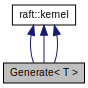
\includegraphics[width=161pt]{class_generate__inherit__graph}
\end{center}
\end{figure}


Collaboration diagram for Generate$<$ T $>$\+:
\nopagebreak
\begin{figure}[H]
\begin{center}
\leavevmode
\includegraphics[width=350pt]{class_generate__coll__graph}
\end{center}
\end{figure}
\subsection*{Public Member Functions}
\begin{DoxyCompactItemize}
\item 
\hypertarget{class_generate_a7c3f2c1b2ae8b2202c5441b60c5f0e6b}{}\label{class_generate_a7c3f2c1b2ae8b2202c5441b60c5f0e6b} 
{\bfseries Generate} (T count=1000)
\item 
virtual raft\+::kstatus \hyperlink{class_generate_aa8253370207e1457b9b79e62253c2925}{run} ()
\end{DoxyCompactItemize}
\subsection*{Additional Inherited Members}


\subsection{Detailed Description}
\subsubsection*{template$<$typename T$>$\newline
class Generate$<$ T $>$}



Definition at line 9 of file brackets\+Test.\+cpp.



\subsection{Member Function Documentation}
\hypertarget{class_generate_aa8253370207e1457b9b79e62253c2925}{}\label{class_generate_aa8253370207e1457b9b79e62253c2925} 
\index{Generate@{Generate}!run@{run}}
\index{run@{run}!Generate@{Generate}}
\subsubsection{\texorpdfstring{run()}{run()}}
{\footnotesize\ttfamily template$<$typename T $>$ \\
virtual raft\+::kstatus \hyperlink{class_generate}{Generate}$<$ T $>$\+::run (\begin{DoxyParamCaption}{ }\end{DoxyParamCaption})\hspace{0.3cm}{\ttfamily [inline]}, {\ttfamily [virtual]}}

run -\/ function to be extended for the actual execution. Code can be executed outside of the run function, i.\+e., with any function call, however the scheduler will only call the run function so it must initiate any follow-\/on behavior desired by the user. else 

Implements \hyperlink{classraft_1_1kernel_a05094286d7577360fb1b91c91fc05901}{raft\+::kernel}.



Definition at line 18 of file brackets\+Test.\+cpp.



References raft\+::map\+::exe().


\begin{DoxyCode}
19    \{
20       \textcolor{keywordflow}{if}( count-- > 1 )
21       \{
22          \textcolor{keyword}{auto} &ref( output[ \textcolor{stringliteral}{"number\_stream"} ].\textcolor{keyword}{template} allocate< T >() );
23          ref = count;
24          output[ \textcolor{stringliteral}{"number\_stream"}].send();
25          
26          \textcolor{keywordflow}{return}( raft::proceed );
27       \}\textcolor{comment}{}
28 \textcolor{comment}{      /** else **/}
29       \textcolor{keyword}{auto} &ref( output[ \textcolor{stringliteral}{"number\_stream"} ].\textcolor{keyword}{template} allocate< T >() );
30       ref = count;
31       output[ \textcolor{stringliteral}{"number\_stream"} ].send( raft::eof );
32       \textcolor{keywordflow}{return}( raft::stop );
33    \}
\end{DoxyCode}
Here is the call graph for this function\+:
\nopagebreak
\begin{figure}[H]
\begin{center}
\leavevmode
\includegraphics[width=350pt]{class_generate_aa8253370207e1457b9b79e62253c2925_cgraph}
\end{center}
\end{figure}


The documentation for this class was generated from the following file\+:\begin{DoxyCompactItemize}
\item 
brackets\+Test.\+cpp\end{DoxyCompactItemize}

\hypertarget{class_graph_tools}{}\section{Graph\+Tools Class Reference}
\label{class_graph_tools}\index{Graph\+Tools@{Graph\+Tools}}
\subsection*{Static Public Member Functions}
\begin{DoxyCompactItemize}
\item 
static void \hyperlink{class_graph_tools_ade51007699cbd681c1a37946609c46ee}{B\+FS} (std\+::set$<$ \hyperlink{classraft_1_1kernel}{raft\+::kernel} $\ast$ $>$ \&source\+\_\+kernels, edge\+\_\+func func, void $\ast$data=nullptr, bool connected\+\_\+error=false)
\item 
static void \hyperlink{class_graph_tools_afc9c2852a351fe8b1a881b5d8b6c97f5}{B\+FS} (std\+::vector$<$ \hyperlink{classraft_1_1kernel}{raft\+::kernel} $\ast$ $>$ \&source\+\_\+kernels, edge\+\_\+func func, void $\ast$data=nullptr, bool connected\+\_\+error=false)
\item 
\hypertarget{class_graph_tools_a4223eca1b9bdb5b2b551f79b1faa155f}{}\label{class_graph_tools_a4223eca1b9bdb5b2b551f79b1faa155f} 
static void {\bfseries B\+FS} (std\+::set$<$ \hyperlink{classraft_1_1kernel}{raft\+::kernel} $\ast$ $>$ \&source\+\_\+kernels, vertex\+\_\+func func, void $\ast$data)
\end{DoxyCompactItemize}


\subsection{Detailed Description}


Definition at line 56 of file graphtools.\+hpp.



\subsection{Member Function Documentation}
\hypertarget{class_graph_tools_ade51007699cbd681c1a37946609c46ee}{}\label{class_graph_tools_ade51007699cbd681c1a37946609c46ee} 
\index{Graph\+Tools@{Graph\+Tools}!B\+FS@{B\+FS}}
\index{B\+FS@{B\+FS}!Graph\+Tools@{Graph\+Tools}}
\subsubsection{\texorpdfstring{B\+F\+S()}{BFS()}\hspace{0.1cm}{\footnotesize\ttfamily [1/2]}}
{\footnotesize\ttfamily void Graph\+Tools\+::\+B\+FS (\begin{DoxyParamCaption}\item[{std\+::set$<$ \hyperlink{classraft_1_1kernel}{raft\+::kernel} $\ast$ $>$ \&}]{source\+\_\+kernels,  }\item[{edge\+\_\+func}]{func,  }\item[{void $\ast$}]{data = {\ttfamily nullptr},  }\item[{bool}]{connected\+\_\+error = {\ttfamily false} }\end{DoxyParamCaption})\hspace{0.3cm}{\ttfamily [static]}}

B\+FS -\/ perform a breadth first search of the graph given by \textquotesingle{}source\+\_\+kernels\textquotesingle{}. The function \textquotesingle{}func\textquotesingle{} matches the typedef above and is called on each edge of the graph exactly once. For state between calls, the user can define a data struct and pass it via the void ptr data which is passed to the func. 
\begin{DoxyParams}{Parameters}
{\em source\+\_\+kernels} & -\/ set of source kernels. \\
\hline
{\em func} & -\/ edge\+\_\+func, funciton to be called \\
\hline
{\em data} & -\/ void$\ast$, data struct for persistent state \\
\hline
{\em connected\+\_\+error,throw} & an error if not connected\\
\hline
\end{DoxyParams}
\hyperlink{graphtools_8cpp_source}{graphtools.\+cpp} -\/ \begin{DoxyAuthor}{Author}
\+: Jonathan Beard 
\end{DoxyAuthor}
\begin{DoxyVersion}{Version}
\+: Sat Sep 20 13\+:15\+:09 2014
\end{DoxyVersion}
Copyright 2014 Jonathan Beard

Licensed under the Apache License, Version 2.\+0 (the \char`\"{}\+License\char`\"{}); you may not use this file except in compliance with the License. You may obtain a copy of the License at\+:

\href{http://www.apache.org/licenses/LICENSE-2.0}{\tt http\+://www.\+apache.\+org/licenses/\+L\+I\+C\+E\+N\+S\+E-\/2.\+0}

Unless required by applicable law or agreed to in writing, software distributed under the License is distributed on an \char`\"{}\+A\+S I\+S\char`\"{} B\+A\+S\+IS, W\+I\+T\+H\+O\+UT W\+A\+R\+R\+A\+N\+T\+I\+ES OR C\+O\+N\+D\+I\+T\+I\+O\+NS OF A\+NY K\+I\+ND, either express or implied. See the License for the specific language governing permissions and limitations under the License. 

Definition at line 38 of file graphtools.\+cpp.



Referenced by B\+F\+S(), raft\+::map\+::check\+Edges(), raft\+::map\+::enable\+Duplication(), dynalloc\+::run(), stdalloc\+::run(), and basic\+\_\+parallel\+::start().


\begin{DoxyCode}
42 \{
43    std::set< raft::kernel* > visited\_set;
44    std::queue< raft::kernel* >     queue;
45    std::for\_each( source\_kernels.begin(),
46                   source\_kernels.end(),
47                   [&]( \hyperlink{classraft_1_1kernel}{raft::kernel} *k )
48                   \{
49                      queue.push( k );
50                      visited\_set.insert( k );
51                   \} );
52    GraphTools::\_\_BFS( queue, visited\_set, func, data, connected\_error );
53 \}
\end{DoxyCode}
\hypertarget{class_graph_tools_afc9c2852a351fe8b1a881b5d8b6c97f5}{}\label{class_graph_tools_afc9c2852a351fe8b1a881b5d8b6c97f5} 
\index{Graph\+Tools@{Graph\+Tools}!B\+FS@{B\+FS}}
\index{B\+FS@{B\+FS}!Graph\+Tools@{Graph\+Tools}}
\subsubsection{\texorpdfstring{B\+F\+S()}{BFS()}\hspace{0.1cm}{\footnotesize\ttfamily [2/2]}}
{\footnotesize\ttfamily void Graph\+Tools\+::\+B\+FS (\begin{DoxyParamCaption}\item[{std\+::vector$<$ \hyperlink{classraft_1_1kernel}{raft\+::kernel} $\ast$ $>$ \&}]{source\+\_\+kernels,  }\item[{edge\+\_\+func}]{func,  }\item[{void $\ast$}]{data = {\ttfamily nullptr},  }\item[{bool}]{connected\+\_\+error = {\ttfamily false} }\end{DoxyParamCaption})\hspace{0.3cm}{\ttfamily [static]}}

B\+FS -\/ perform a breadth first search of the graph given by \textquotesingle{}source\+\_\+kernels\textquotesingle{}. The function \textquotesingle{}func\textquotesingle{} matches the typedef above and is called on each edge of the graph exactly once. For state between calls, the user can define a data struct and pass it via the void ptr data which is passed to the func. 
\begin{DoxyParams}{Parameters}
{\em source\+\_\+kernels} & -\/ set of source kernels. \\
\hline
{\em func} & -\/ edge\+\_\+func, funciton to be called \\
\hline
{\em data} & -\/ void$\ast$, data struct for persistent state \\
\hline
{\em connected\+\_\+error,throw} & an error if not connected \\
\hline
\end{DoxyParams}


Definition at line 56 of file graphtools.\+cpp.



References B\+F\+S(), Port\+::get\+Port\+Info\+For(), raft\+::kernel\+::input, Port\+::portmap, and common\+::print\+Class\+Name().


\begin{DoxyCode}
60 \{
61    std::set< raft::kernel* >       visited\_set;
62    std::queue< raft::kernel* >     queue;
63    std::for\_each( source\_kernels.begin(),
64                   source\_kernels.end(),
65                   [&]( \hyperlink{classraft_1_1kernel}{raft::kernel} *k )
66                   \{
67                      queue.push( k );
68                      visited\_set.insert( k );
69                   \} );
70    GraphTools::\_\_BFS( queue, visited\_set, func, data, connected\_error );
71 \}
\end{DoxyCode}
Here is the call graph for this function\+:
\nopagebreak
\begin{figure}[H]
\begin{center}
\leavevmode
\includegraphics[width=350pt]{class_graph_tools_afc9c2852a351fe8b1a881b5d8b6c97f5_cgraph}
\end{center}
\end{figure}


The documentation for this class was generated from the following files\+:\begin{DoxyCompactItemize}
\item 
graphtools.\+hpp\item 
graphtools.\+cpp\end{DoxyCompactItemize}

\hypertarget{classinterface__partition}{}\section{interface\+\_\+partition Class Reference}
\label{classinterface__partition}\index{interface\+\_\+partition@{interface\+\_\+partition}}


{\ttfamily \#include $<$interface\+\_\+partition.\+hpp$>$}



Inheritance diagram for interface\+\_\+partition\+:
\nopagebreak
\begin{figure}[H]
\begin{center}
\leavevmode
\includegraphics[width=268pt]{classinterface__partition__inherit__graph}
\end{center}
\end{figure}
\subsection*{Public Member Functions}
\begin{DoxyCompactItemize}
\item 
virtual void \hyperlink{classinterface__partition_a7161f6277517624347fda38c8ffa019d}{partition} (kernelkeeper \&keeper)=0
\end{DoxyCompactItemize}
\subsection*{Static Protected Member Functions}
\begin{DoxyCompactItemize}
\item 
{\footnotesize template$<$class T , class C\+O\+RE $>$ }\\static void \hyperlink{classinterface__partition_af7c257c87d13508274e934328ee90f52}{set\+Core} (T \&kernel, const C\+O\+RE core)
\end{DoxyCompactItemize}


\subsection{Detailed Description}
\hyperlink{interface__partition_8hpp_source}{interface\+\_\+partition.\+hpp} -\/ interface for all the kernel partitioners within Raft\+Lib \begin{DoxyAuthor}{Author}
\+: Jonathan Beard 
\end{DoxyAuthor}
\begin{DoxyVersion}{Version}
\+: Tue May 3 12\+:43\+:22 2016
\end{DoxyVersion}
Copyright 2016 Jonathan Beard

Licensed under the Apache License, Version 2.\+0 (the \char`\"{}\+License\char`\"{}); you may not use this file except in compliance with the License. You may obtain a copy of the License at\+:

\href{http://www.apache.org/licenses/LICENSE-2.0}{\tt http\+://www.\+apache.\+org/licenses/\+L\+I\+C\+E\+N\+S\+E-\/2.\+0}

Unless required by applicable law or agreed to in writing, software distributed under the License is distributed on an \char`\"{}\+A\+S I\+S\char`\"{} B\+A\+S\+IS, W\+I\+T\+H\+O\+UT W\+A\+R\+R\+A\+N\+T\+I\+ES OR C\+O\+N\+D\+I\+T\+I\+O\+NS OF A\+NY K\+I\+ND, either express or implied. See the License for the specific language governing permissions and limitations under the License. 

Definition at line 27 of file interface\+\_\+partition.\+hpp.



\subsection{Member Function Documentation}
\hypertarget{classinterface__partition_a7161f6277517624347fda38c8ffa019d}{}\label{classinterface__partition_a7161f6277517624347fda38c8ffa019d} 
\index{interface\+\_\+partition@{interface\+\_\+partition}!partition@{partition}}
\index{partition@{partition}!interface\+\_\+partition@{interface\+\_\+partition}}
\subsubsection{\texorpdfstring{partition()}{partition()}}
{\footnotesize\ttfamily virtual void interface\+\_\+partition\+::partition (\begin{DoxyParamCaption}\item[{kernelkeeper \&}]{keeper }\end{DoxyParamCaption})\hspace{0.3cm}{\ttfamily [pure virtual]}}

partition -\/ call me to activate the partitioning algorithm. The kernel objects are all that you should need. there\textquotesingle{}s a core assignment variable that can map back via the run-\/time to the hardware type if need be. 
\begin{DoxyParams}{Parameters}
{\em kernels} & -\/ kernelkeeper\& \\
\hline
\end{DoxyParams}


Implemented in \hyperlink{classpartition__basic_a3dc4106326788887f9a7c6ac49bb46d4}{partition\+\_\+basic}, and \hyperlink{classpartition__dummy_ae40e5fa9d982e718f399fe3244435e7a}{partition\+\_\+dummy}.

\hypertarget{classinterface__partition_af7c257c87d13508274e934328ee90f52}{}\label{classinterface__partition_af7c257c87d13508274e934328ee90f52} 
\index{interface\+\_\+partition@{interface\+\_\+partition}!set\+Core@{set\+Core}}
\index{set\+Core@{set\+Core}!interface\+\_\+partition@{interface\+\_\+partition}}
\subsubsection{\texorpdfstring{set\+Core()}{setCore()}}
{\footnotesize\ttfamily template$<$class T , class C\+O\+RE $>$ \\
static void interface\+\_\+partition\+::set\+Core (\begin{DoxyParamCaption}\item[{T \&}]{kernel,  }\item[{const C\+O\+RE}]{core }\end{DoxyParamCaption})\hspace{0.3cm}{\ttfamily [inline]}, {\ttfamily [static]}, {\ttfamily [protected]}}

T\+O\+DO\+: add std\+::enable\+\_\+if 

Definition at line 47 of file interface\+\_\+partition.\+hpp.



Referenced by partition\+\_\+basic\+::partition().


\begin{DoxyCode}
48     \{
49         kernel.setCore( core );
50         \textcolor{keywordflow}{return};
51     \}
\end{DoxyCode}


The documentation for this class was generated from the following file\+:\begin{DoxyCompactItemize}
\item 
interface\+\_\+partition.\+hpp\end{DoxyCompactItemize}

\hypertarget{class_invalid_topology_operation_exception}{}\section{Invalid\+Topology\+Operation\+Exception Class Reference}
\label{class_invalid_topology_operation_exception}\index{Invalid\+Topology\+Operation\+Exception@{Invalid\+Topology\+Operation\+Exception}}


Inheritance diagram for Invalid\+Topology\+Operation\+Exception\+:
\nopagebreak
\begin{figure}[H]
\begin{center}
\leavevmode
\includegraphics[width=209pt]{class_invalid_topology_operation_exception__inherit__graph}
\end{center}
\end{figure}


Collaboration diagram for Invalid\+Topology\+Operation\+Exception\+:
\nopagebreak
\begin{figure}[H]
\begin{center}
\leavevmode
\includegraphics[width=209pt]{class_invalid_topology_operation_exception__coll__graph}
\end{center}
\end{figure}
\subsection*{Public Member Functions}
\begin{DoxyCompactItemize}
\item 
\hypertarget{class_invalid_topology_operation_exception_aa3e3b3739915daf9e1f6fda503e9aee2}{}\label{class_invalid_topology_operation_exception_aa3e3b3739915daf9e1f6fda503e9aee2} 
{\bfseries Invalid\+Topology\+Operation\+Exception} (const std\+::string message)
\end{DoxyCompactItemize}


\subsection{Detailed Description}


Definition at line 36 of file mapexception.\+hpp.



The documentation for this class was generated from the following file\+:\begin{DoxyCompactItemize}
\item 
mapexception.\+hpp\end{DoxyCompactItemize}

\hypertarget{classraft_1_1join}{}\section{raft\+:\+:join$<$ T, method $>$ Class Template Reference}
\label{classraft_1_1join}\index{raft\+::join$<$ T, method $>$@{raft\+::join$<$ T, method $>$}}


The documentation for this class was generated from the following file\+:\begin{DoxyCompactItemize}
\item 
port.\+hpp\end{DoxyCompactItemize}

\hypertarget{classraft_1_1kernel}{}\section{raft\+:\+:kernel Class Reference}
\label{classraft_1_1kernel}\index{raft\+::kernel@{raft\+::kernel}}


Inheritance diagram for raft\+:\+:kernel\+:
\nopagebreak
\begin{figure}[H]
\begin{center}
\leavevmode
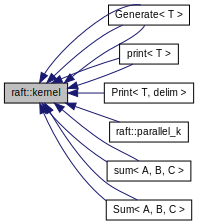
\includegraphics[width=264pt]{classraft_1_1kernel__inherit__graph}
\end{center}
\end{figure}


Collaboration diagram for raft\+:\+:kernel\+:
\nopagebreak
\begin{figure}[H]
\begin{center}
\leavevmode
\includegraphics[width=350pt]{classraft_1_1kernel__coll__graph}
\end{center}
\end{figure}
\subsection*{Public Member Functions}
\begin{DoxyCompactItemize}
\item 
\hyperlink{classraft_1_1kernel_a57aa6c7842f594d1522fb1c127fc4588}{kernel} ()
\item 
\hyperlink{classraft_1_1kernel_a8c275f04f04b99d77fc4639a053112c8}{kernel} (void $\ast$const ptr, const std\+::size\+\_\+t nbytes)
\item 
virtual raft\+::kstatus \hyperlink{classraft_1_1kernel_a05094286d7577360fb1b91c91fc05901}{run} ()=0
\item 
virtual \hyperlink{classraft_1_1kernel}{raft\+::kernel} $\ast$ \hyperlink{classraft_1_1kernel_a71bfffbbb3d40949e19be32e3d8f467f}{clone} ()
\item 
\hypertarget{classraft_1_1kernel_a2376ee5c5d413955db3f017fb707a6df}{}\label{classraft_1_1kernel_a2376ee5c5d413955db3f017fb707a6df} 
std\+::size\+\_\+t {\bfseries get\+\_\+id} ()
\item 
\hyperlink{classraft_1_1kernel}{raft\+::kernel} \& \hyperlink{classraft_1_1kernel_a186ea784c5b1ac8fd90f2112c1c62675}{operator\mbox{[}$\,$\mbox{]}} (const std\+::string \&\&portname)
\item 
\hypertarget{classraft_1_1kernel_aafd70e8e6ff6137db295e8dd0388b77d}{}\label{classraft_1_1kernel_aafd70e8e6ff6137db295e8dd0388b77d} 
core\+\_\+id\+\_\+t {\bfseries get\+Core\+Assignment} () noexcept
\end{DoxyCompactItemize}
\subsection*{Static Public Member Functions}
\begin{DoxyCompactItemize}
\item 
\hypertarget{classraft_1_1kernel_aebbcef35d4e08abbbe4167c2b75fab5f}{}\label{classraft_1_1kernel_aebbcef35d4e08abbbe4167c2b75fab5f} 
{\footnotesize template$<$class T , class ... Args$>$ }\\static \hyperlink{classraft_1_1kernel__wrapper}{kernel\+\_\+wrapper} {\bfseries make} (Args \&\&... params)
\end{DoxyCompactItemize}
\subsection*{Protected Member Functions}
\begin{DoxyCompactItemize}
\item 
\hypertarget{classraft_1_1kernel_ab206ff6ee1b729ab8875e181cbef227f}{}\label{classraft_1_1kernel_ab206ff6ee1b729ab8875e181cbef227f} 
virtual std\+::size\+\_\+t {\bfseries add\+Port} ()
\item 
virtual void \hyperlink{classraft_1_1kernel_abd7f3bf1f689840f7d61f472f520c258}{lock} ()
\item 
virtual void \hyperlink{classraft_1_1kernel_a7966dcabb0ed65ac52f6f78918256861}{unlock} ()
\item 
\hypertarget{classraft_1_1kernel_ad463ccfdb7d7e5360cba78bec277cbfe}{}\label{classraft_1_1kernel_ad463ccfdb7d7e5360cba78bec277cbfe} 
std\+::string {\bfseries get\+Enabled\+Port} ()
\item 
\hypertarget{classraft_1_1kernel_a0615a961de9038101c266e69fe2994ca}{}\label{classraft_1_1kernel_a0615a961de9038101c266e69fe2994ca} 
void {\bfseries retire} () noexcept
\item 
\hypertarget{classraft_1_1kernel_a41f090e0b3a4cf96471207155f6af80a}{}\label{classraft_1_1kernel_a41f090e0b3a4cf96471207155f6af80a} 
bool {\bfseries is\+Retired} () noexcept
\item 
\hypertarget{classraft_1_1kernel_a070219cf511c97848218a3431952395c}{}\label{classraft_1_1kernel_a070219cf511c97848218a3431952395c} 
void {\bfseries set\+Core} (const core\+\_\+id\+\_\+t id) noexcept
\end{DoxyCompactItemize}
\subsection*{Protected Attributes}
\begin{DoxyCompactItemize}
\item 
\hyperlink{class_port}{Port} \hyperlink{classraft_1_1kernel_a6edbe35a56409d402e719b3ac36d6554}{input} = \{ this \}
\item 
\hypertarget{classraft_1_1kernel_a1c65cc76ecaa8880ba527e5a146ca4ba}{}\label{classraft_1_1kernel_a1c65cc76ecaa8880ba527e5a146ca4ba} 
\hyperlink{class_port}{Port} {\bfseries output} = \{ this \}
\item 
\hypertarget{classraft_1_1kernel_afc8b7b8a99c538a5f741309730832fc4}{}\label{classraft_1_1kernel_afc8b7b8a99c538a5f741309730832fc4} 
bool {\bfseries internal\+\_\+alloc} = false
\item 
\hypertarget{classraft_1_1kernel_af754bdc01acf6eea572d0ddcd89b568f}{}\label{classraft_1_1kernel_af754bdc01acf6eea572d0ddcd89b568f} 
core\+\_\+id\+\_\+t {\bfseries core\+\_\+assign} = -\/1
\end{DoxyCompactItemize}
\subsection*{Static Protected Attributes}
\begin{DoxyCompactItemize}
\item 
static std\+::size\+\_\+t \hyperlink{classraft_1_1kernel_a98e05f7418c208e28b9112e92df7eccf}{kernel\+\_\+count}
\end{DoxyCompactItemize}
\subsection*{Friends}
\begin{DoxyCompactItemize}
\item 
class \hyperlink{classraft_1_1kernel_aeda338414e516b47761f994fb78056c6}{map}
\item 
class \hyperlink{classraft_1_1kernel_a1045638a7591b3c72cd145fc541d6478}{\+::\+Map\+Base}
\item 
\hypertarget{classraft_1_1kernel_a59b0d31ff28240338a2b6e682030ca3c}{}\label{classraft_1_1kernel_a59b0d31ff28240338a2b6e682030ca3c} 
class {\bfseries \+::\+Schedule}
\item 
\hypertarget{classraft_1_1kernel_a24755791643232aebfeedaa4ff0ecf03}{}\label{classraft_1_1kernel_a24755791643232aebfeedaa4ff0ecf03} 
class {\bfseries \+::\+Graph\+Tools}
\item 
\hypertarget{classraft_1_1kernel_aa3a6c191bed2aef9502f837b67e786b2}{}\label{classraft_1_1kernel_aa3a6c191bed2aef9502f837b67e786b2} 
class {\bfseries \+::kernel\+\_\+container}
\item 
\hypertarget{classraft_1_1kernel_ae75d52e84ecfc11bcaa43dd9fe149a2f}{}\label{classraft_1_1kernel_ae75d52e84ecfc11bcaa43dd9fe149a2f} 
class {\bfseries \+::basic\+\_\+parallel}
\item 
\hypertarget{classraft_1_1kernel_ae07b02dff85bd74c2d4d69d55bafe0a2}{}\label{classraft_1_1kernel_ae07b02dff85bd74c2d4d69d55bafe0a2} 
class {\bfseries \+::kpair}
\item 
\hypertarget{classraft_1_1kernel_a6b0f0238fe633a6ff44089d4667d3a7a}{}\label{classraft_1_1kernel_a6b0f0238fe633a6ff44089d4667d3a7a} 
class {\bfseries \+::interface\+\_\+partition}
\item 
\hypertarget{classraft_1_1kernel_a24b9e107a2ae5dbaf9831c0acc54df32}{}\label{classraft_1_1kernel_a24b9e107a2ae5dbaf9831c0acc54df32} 
class {\bfseries \+::pool\+\_\+schedule}
\end{DoxyCompactItemize}


\subsection{Detailed Description}


Definition at line 64 of file kernel.\+hpp.



\subsection{Constructor \& Destructor Documentation}
\hypertarget{classraft_1_1kernel_a57aa6c7842f594d1522fb1c127fc4588}{}\label{classraft_1_1kernel_a57aa6c7842f594d1522fb1c127fc4588} 
\index{raft\+::kernel@{raft\+::kernel}!kernel@{kernel}}
\index{kernel@{kernel}!raft\+::kernel@{raft\+::kernel}}
\subsubsection{\texorpdfstring{kernel()}{kernel()}\hspace{0.1cm}{\footnotesize\ttfamily [1/2]}}
{\footnotesize\ttfamily kernel\+::kernel (\begin{DoxyParamCaption}{ }\end{DoxyParamCaption})}

default constructor

default 

Definition at line 10 of file kernel.\+cpp.



References kernel\+\_\+count.


\begin{DoxyCode}
10                : kernel\_id( \hyperlink{classraft_1_1kernel_a98e05f7418c208e28b9112e92df7eccf}{kernel::kernel\_count} )
11 \{
12    \hyperlink{classraft_1_1kernel_a98e05f7418c208e28b9112e92df7eccf}{kernel::kernel\_count}++;
13 \}
\end{DoxyCode}
\hypertarget{classraft_1_1kernel_a8c275f04f04b99d77fc4639a053112c8}{}\label{classraft_1_1kernel_a8c275f04f04b99d77fc4639a053112c8} 
\index{raft\+::kernel@{raft\+::kernel}!kernel@{kernel}}
\index{kernel@{kernel}!raft\+::kernel@{raft\+::kernel}}
\subsubsection{\texorpdfstring{kernel()}{kernel()}\hspace{0.1cm}{\footnotesize\ttfamily [2/2]}}
{\footnotesize\ttfamily kernel\+::kernel (\begin{DoxyParamCaption}\item[{void $\ast$const}]{ptr,  }\item[{const std\+::size\+\_\+t}]{nbytes }\end{DoxyParamCaption})}

in-\/place allocation

existing memory 

Definition at line 16 of file kernel.\+cpp.


\begin{DoxyCode}
17                                          :
18    \hyperlink{classraft_1_1kernel_a6edbe35a56409d402e719b3ac36d6554}{input}(  \textcolor{keyword}{this}, ptr, nbytes ),
19    output( \textcolor{keyword}{this}, ptr, nbytes ),
20    kernel\_id( \hyperlink{classraft_1_1kernel_a98e05f7418c208e28b9112e92df7eccf}{kernel::kernel\_count} )
21 \{
22 \}
\end{DoxyCode}


\subsection{Member Function Documentation}
\hypertarget{classraft_1_1kernel_a71bfffbbb3d40949e19be32e3d8f467f}{}\label{classraft_1_1kernel_a71bfffbbb3d40949e19be32e3d8f467f} 
\index{raft\+::kernel@{raft\+::kernel}!clone@{clone}}
\index{clone@{clone}!raft\+::kernel@{raft\+::kernel}}
\subsubsection{\texorpdfstring{clone()}{clone()}}
{\footnotesize\ttfamily virtual \hyperlink{classraft_1_1kernel}{raft\+::kernel}$\ast$ raft\+::kernel\+::clone (\begin{DoxyParamCaption}{ }\end{DoxyParamCaption})\hspace{0.3cm}{\ttfamily [inline]}, {\ttfamily [virtual]}}

clone -\/ used for parallelization of kernels, if necessary sub-\/kernels should include an appropriate copy constructor so all class member variables can be set. 
\begin{DoxyParams}{Parameters}
{\em other,T\&} & -\/ reference to object to be cloned \\
\hline
\end{DoxyParams}
\begin{DoxyReturn}{Returns}
kernel$\ast$ -\/ takes base type, however is same as allocated by copy constructor for T. 
\end{DoxyReturn}
won\textquotesingle{}t be reached 

Definition at line 105 of file kernel.\+hpp.



References lock(), operator\mbox{[}$\,$\mbox{]}(), and unlock().



Referenced by raft\+::map\+::operator+=(), and basic\+\_\+parallel\+::start().


\begin{DoxyCode}
106    \{
107       \textcolor{keywordflow}{throw} \hyperlink{class_clone_not_implemented_exception}{CloneNotImplementedException}( \textcolor{stringliteral}{"Sub-class has failed to implement
       clone function, please use the CLONE() macro to add functionality"} );\textcolor{comment}{}
108 \textcolor{comment}{      /** won't be reached **/}
109       \textcolor{keywordflow}{return}( \textcolor{keyword}{nullptr} );
110    \}
\end{DoxyCode}
Here is the call graph for this function\+:
\nopagebreak
\begin{figure}[H]
\begin{center}
\leavevmode
\includegraphics[width=320pt]{classraft_1_1kernel_a71bfffbbb3d40949e19be32e3d8f467f_cgraph}
\end{center}
\end{figure}
\hypertarget{classraft_1_1kernel_abd7f3bf1f689840f7d61f472f520c258}{}\label{classraft_1_1kernel_abd7f3bf1f689840f7d61f472f520c258} 
\index{raft\+::kernel@{raft\+::kernel}!lock@{lock}}
\index{lock@{lock}!raft\+::kernel@{raft\+::kernel}}
\subsubsection{\texorpdfstring{lock()}{lock()}}
{\footnotesize\ttfamily void kernel\+::lock (\begin{DoxyParamCaption}{ }\end{DoxyParamCaption})\hspace{0.3cm}{\ttfamily [protected]}, {\ttfamily [virtual]}}

does nothing, just need a base impl 

Definition at line 54 of file kernel.\+cpp.



Referenced by clone().


\begin{DoxyCode}
55 \{\textcolor{comment}{}
56 \textcolor{comment}{   /** does nothing, just need a base impl **/}
57    \textcolor{keywordflow}{return};
58 \}
\end{DoxyCode}
\hypertarget{classraft_1_1kernel_a186ea784c5b1ac8fd90f2112c1c62675}{}\label{classraft_1_1kernel_a186ea784c5b1ac8fd90f2112c1c62675} 
\index{raft\+::kernel@{raft\+::kernel}!operator\mbox{[}\mbox{]}@{operator[]}}
\index{operator\mbox{[}\mbox{]}@{operator[]}!raft\+::kernel@{raft\+::kernel}}
\subsubsection{\texorpdfstring{operator[]()}{operator[]()}}
{\footnotesize\ttfamily \hyperlink{classraft_1_1kernel}{raft\+::kernel} \& kernel\+::operator\mbox{[}$\,$\mbox{]} (\begin{DoxyParamCaption}\item[{const std\+::string \&\&}]{portname }\end{DoxyParamCaption})}

operator\mbox{[}\mbox{]} -\/ returns the current kernel with the specified port name enabled for linking. 
\begin{DoxyParams}{Parameters}
{\em portname} & -\/ const std\+::string\&\& \\
\hline
\end{DoxyParams}
\begin{DoxyReturn}{Returns}
\hyperlink{classraft_1_1kernel}{raft\+::kernel}\&\& 
\end{DoxyReturn}


Definition at line 32 of file kernel.\+cpp.



Referenced by clone().


\begin{DoxyCode}
33 \{
34    \textcolor{keywordflow}{if}( enabled\_port.size() < 2 )
35    \{
36         enabled\_port.push( portname );
37    \}
38    \textcolor{keywordflow}{else}
39    \{
40         \textcolor{keywordflow}{throw} \hyperlink{class_ambiguous_port_assignment_exception}{AmbiguousPortAssignmentException}(
41             \textcolor{stringliteral}{"too many ports added with: "} + portname
42         );
43    \}
44    \textcolor{keywordflow}{return}( (*\textcolor{keyword}{this}) );
45 \}
\end{DoxyCode}
\hypertarget{classraft_1_1kernel_a05094286d7577360fb1b91c91fc05901}{}\label{classraft_1_1kernel_a05094286d7577360fb1b91c91fc05901} 
\index{raft\+::kernel@{raft\+::kernel}!run@{run}}
\index{run@{run}!raft\+::kernel@{raft\+::kernel}}
\subsubsection{\texorpdfstring{run()}{run()}}
{\footnotesize\ttfamily virtual raft\+::kstatus raft\+::kernel\+::run (\begin{DoxyParamCaption}{ }\end{DoxyParamCaption})\hspace{0.3cm}{\ttfamily [pure virtual]}}

run -\/ function to be extended for the actual execution. Code can be executed outside of the run function, i.\+e., with any function call, however the scheduler will only call the run function so it must initiate any follow-\/on behavior desired by the user. 

Implemented in \hyperlink{classlast_a7a1da1c30f571a8e8ccb515ca2cb2f02}{last}, \hyperlink{classlast_a7a1da1c30f571a8e8ccb515ca2cb2f02}{last}, \hyperlink{classlast_a7a1da1c30f571a8e8ccb515ca2cb2f02}{last}, \hyperlink{classlast_a7a1da1c30f571a8e8ccb515ca2cb2f02}{last}, \hyperlink{classmiddle_a9aa7415c102af751be9c7af4771b6f16}{middle}, \hyperlink{classlast_a7a1da1c30f571a8e8ccb515ca2cb2f02}{last}, \hyperlink{classmiddle_a9aa7415c102af751be9c7af4771b6f16}{middle}, \hyperlink{classmiddle_a9aa7415c102af751be9c7af4771b6f16}{middle}, \hyperlink{classmiddle_a9aa7415c102af751be9c7af4771b6f16}{middle}, \hyperlink{classlast_a7a1da1c30f571a8e8ccb515ca2cb2f02}{last}, \hyperlink{classstart_a4c076d756e2846f51e54452853a9ed6d}{start}, \hyperlink{classstart_a4c076d756e2846f51e54452853a9ed6d}{start}, \hyperlink{classstart_a4c076d756e2846f51e54452853a9ed6d}{start}, \hyperlink{classstart_a4c076d756e2846f51e54452853a9ed6d}{start}, \hyperlink{classstart_a4c076d756e2846f51e54452853a9ed6d}{start}, \hyperlink{classsub_a0a0c7461433ee8b5f4b24305282bf69a}{sub$<$ T $>$}, \hyperlink{classdisplay_a8652ca329ee5d1650e183b17f7299b51}{display$<$ T $>$}, \hyperlink{classsub_a0a0c7461433ee8b5f4b24305282bf69a}{sub$<$ T $>$}, \hyperlink{classsub_a0a0c7461433ee8b5f4b24305282bf69a}{sub$<$ T $>$}, \hyperlink{classsub_a0a0c7461433ee8b5f4b24305282bf69a}{sub$<$ T $>$}, \hyperlink{classsub_a0a0c7461433ee8b5f4b24305282bf69a}{sub$<$ T $>$}, \hyperlink{classsub_a0a0c7461433ee8b5f4b24305282bf69a}{sub$<$ T $>$}, \hyperlink{classsub_a0a0c7461433ee8b5f4b24305282bf69a}{sub$<$ T $>$}, \hyperlink{classsub_a0a0c7461433ee8b5f4b24305282bf69a}{sub$<$ T $>$}, \hyperlink{classsub_a0a0c7461433ee8b5f4b24305282bf69a}{sub$<$ T $>$}, \hyperlink{classsub_a0a0c7461433ee8b5f4b24305282bf69a}{sub$<$ T $>$}, \hyperlink{classsub_a0a0c7461433ee8b5f4b24305282bf69a}{sub$<$ T $>$}, \hyperlink{classsub_a0a0c7461433ee8b5f4b24305282bf69a}{sub$<$ T $>$}, \hyperlink{classstart_a4c076d756e2846f51e54452853a9ed6d}{start}, \hyperlink{classsource_ad144988607882cbe591a4c71642cb77a}{source$<$ T $>$}, \hyperlink{class_sum_ab915892675d11a8f3f0de2e7f96b0d28}{Sum$<$ A, B, C $>$}, \hyperlink{class_sum_ab915892675d11a8f3f0de2e7f96b0d28}{Sum$<$ A, B, C $>$}, \hyperlink{class_sum_ab915892675d11a8f3f0de2e7f96b0d28}{Sum$<$ A, B, C $>$}, \hyperlink{classprint_aa547f61c584b4044e4a0dfc2410e5adc}{print$<$ T $>$}, \hyperlink{class_generate_aa8253370207e1457b9b79e62253c2925}{Generate$<$ T $>$}, and \hyperlink{classsum_a2d0fac9129b826678d00520621937b15}{sum$<$ T $>$}.



Referenced by Schedule\+::kernel\+Run().

\hypertarget{classraft_1_1kernel_a7966dcabb0ed65ac52f6f78918256861}{}\label{classraft_1_1kernel_a7966dcabb0ed65ac52f6f78918256861} 
\index{raft\+::kernel@{raft\+::kernel}!unlock@{unlock}}
\index{unlock@{unlock}!raft\+::kernel@{raft\+::kernel}}
\subsubsection{\texorpdfstring{unlock()}{unlock()}}
{\footnotesize\ttfamily void kernel\+::unlock (\begin{DoxyParamCaption}{ }\end{DoxyParamCaption})\hspace{0.3cm}{\ttfamily [protected]}, {\ttfamily [virtual]}}

does nothing, just need a base impl 

Definition at line 61 of file kernel.\+cpp.



Referenced by clone().


\begin{DoxyCode}
62 \{\textcolor{comment}{}
63 \textcolor{comment}{   /** does nothing, just need a base impl **/}
64    \textcolor{keywordflow}{return};
65 \}
\end{DoxyCode}


\subsection{Friends And Related Function Documentation}
\hypertarget{classraft_1_1kernel_a1045638a7591b3c72cd145fc541d6478}{}\label{classraft_1_1kernel_a1045638a7591b3c72cd145fc541d6478} 
\index{raft\+::kernel@{raft\+::kernel}!\+::\+Map\+Base@{\+::\+Map\+Base}}
\index{\+::\+Map\+Base@{\+::\+Map\+Base}!raft\+::kernel@{raft\+::kernel}}
\subsubsection{\texorpdfstring{\+::\+Map\+Base}{::MapBase}}
{\footnotesize\ttfamily friend class \+::\hyperlink{class_map_base}{Map\+Base}\hspace{0.3cm}{\ttfamily [friend]}}

in global namespace 

Definition at line 149 of file kernel.\+hpp.

\hypertarget{classraft_1_1kernel_aeda338414e516b47761f994fb78056c6}{}\label{classraft_1_1kernel_aeda338414e516b47761f994fb78056c6} 
\index{raft\+::kernel@{raft\+::kernel}!map@{map}}
\index{map@{map}!raft\+::kernel@{raft\+::kernel}}
\subsubsection{\texorpdfstring{map}{map}}
{\footnotesize\ttfamily friend class \hyperlink{classraft_1_1map}{map}\hspace{0.3cm}{\ttfamily [friend]}}

in namespace raft 

Definition at line 147 of file kernel.\+hpp.



\subsection{Member Data Documentation}
\hypertarget{classraft_1_1kernel_a6edbe35a56409d402e719b3ac36d6554}{}\label{classraft_1_1kernel_a6edbe35a56409d402e719b3ac36d6554} 
\index{raft\+::kernel@{raft\+::kernel}!input@{input}}
\index{input@{input}!raft\+::kernel@{raft\+::kernel}}
\subsubsection{\texorpdfstring{input}{input}}
{\footnotesize\ttfamily \hyperlink{class_port}{Port} raft\+::kernel\+::input = \{ this \}\hspace{0.3cm}{\ttfamily [protected]}}

P\+O\+R\+TS -\/ input and output, use these to interact with the outside world. 

Definition at line 140 of file kernel.\+hpp.



Referenced by Graph\+Tools\+::\+B\+F\+S(), Schedule\+::check\+System\+Signal(), raft\+::map\+::enable\+Duplication(), Map\+Base\+::join(), Schedule\+::kernel\+Has\+Input\+Data(), Schedule\+::kernel\+Has\+No\+Input\+Ports(), kpair\+::kpair(), Map\+Base\+::link(), raft\+::map\+::operator+=(), sum$<$ T $>$\+::run(), print$<$ T $>$\+::run(), Sum$<$ A, B, C $>$\+::run(), start\+::run(), sub$<$ T $>$\+::run(), display$<$ T $>$\+::run(), last\+::run(), Schedule\+::schedule\+Kernel(), Schedule\+::set\+Ptr\+Sets(), and basic\+\_\+parallel\+::start().

\hypertarget{classraft_1_1kernel_a98e05f7418c208e28b9112e92df7eccf}{}\label{classraft_1_1kernel_a98e05f7418c208e28b9112e92df7eccf} 
\index{raft\+::kernel@{raft\+::kernel}!kernel\+\_\+count@{kernel\+\_\+count}}
\index{kernel\+\_\+count@{kernel\+\_\+count}!raft\+::kernel@{raft\+::kernel}}
\subsubsection{\texorpdfstring{kernel\+\_\+count}{kernel\_count}}
{\footnotesize\ttfamily std\+::size\+\_\+t kernel\+::kernel\+\_\+count\hspace{0.3cm}{\ttfamily [static]}, {\ttfamily [protected]}}

N\+O\+TE\+: doesn\textquotesingle{}t need to be atomic since only one thread will have responsibility to to create new compute kernels. 

Definition at line 163 of file kernel.\+hpp.



Referenced by kernel().



The documentation for this class was generated from the following files\+:\begin{DoxyCompactItemize}
\item 
kernel.\+hpp\item 
kernel.\+cpp\end{DoxyCompactItemize}

\hypertarget{classkernel__container}{}\section{kernel\+\_\+container Class Reference}
\label{classkernel__container}\index{kernel\+\_\+container@{kernel\+\_\+container}}
\subsection*{Public Types}
\begin{DoxyCompactItemize}
\item 
\hypertarget{classkernel__container_aaa8403088c93fca461e37158069d91b5}{}\label{classkernel__container_aaa8403088c93fca461e37158069d91b5} 
using {\bfseries buffer} = Ring\+Buffer$<$ \hyperlink{structsched__cmd__t}{sched\+\_\+cmd\+\_\+t}, Type\+::\+Ring\+Buffer\+Type\+::\+Heap, false $>$
\end{DoxyCompactItemize}
\subsection*{Public Member Functions}
\begin{DoxyCompactItemize}
\item 
\hyperlink{classkernel__container_a273d59eff9b9e269f1f9b231abc37b83}{kernel\+\_\+container} ()
\item 
\hyperlink{classkernel__container_a6d97cddd3d2f015166485afad9c71ff5}{kernel\+\_\+container} (const std\+::size\+\_\+t N)
\item 
\hyperlink{classkernel__container_acec164e3f4c6f37f4791c90c24514b34}{$\sim$kernel\+\_\+container} ()
\item 
buffer \& \hyperlink{classkernel__container_abcbec3854917b37bd6421b6b8ed2c2c0}{get\+Input\+Queue} ()
\item 
buffer \& \hyperlink{classkernel__container_a64384e258fee9b664d164eb50baf33df}{get\+Output\+Queue} ()
\item 
std\+::size\+\_\+t \hyperlink{classkernel__container_a358a15b772f1b7dfa57bd733fc78fcaa}{size} ()
\end{DoxyCompactItemize}
\subsection*{Static Public Member Functions}
\begin{DoxyCompactItemize}
\item 
static void \hyperlink{classkernel__container_a89f9b11119d9ab0e8c64215bf50856f0}{container\+\_\+run} (\hyperlink{classkernel__container}{kernel\+\_\+container} \&container)
\end{DoxyCompactItemize}


\subsection{Detailed Description}


Definition at line 36 of file kernelcontainer.\+hpp.



\subsection{Constructor \& Destructor Documentation}
\hypertarget{classkernel__container_a273d59eff9b9e269f1f9b231abc37b83}{}\label{classkernel__container_a273d59eff9b9e269f1f9b231abc37b83} 
\index{kernel\+\_\+container@{kernel\+\_\+container}!kernel\+\_\+container@{kernel\+\_\+container}}
\index{kernel\+\_\+container@{kernel\+\_\+container}!kernel\+\_\+container@{kernel\+\_\+container}}
\subsubsection{\texorpdfstring{kernel\+\_\+container()}{kernel\_container()}\hspace{0.1cm}{\footnotesize\ttfamily [1/2]}}
{\footnotesize\ttfamily kernel\+\_\+container\+::kernel\+\_\+container (\begin{DoxyParamCaption}{ }\end{DoxyParamCaption})}

\hyperlink{classkernel__container}{kernel\+\_\+container} -\/ default constructor, initializes all above pointers.

\hyperlink{kernelcontainer_8cpp_source}{kernelcontainer.\+cpp} -\/ \begin{DoxyAuthor}{Author}
\+: Jonathan Beard 
\end{DoxyAuthor}
\begin{DoxyVersion}{Version}
\+: Sun Mar 22 09\+:13\+:32 2015
\end{DoxyVersion}
Copyright 2015 Jonathan Beard

Licensed under the Apache License, Version 2.\+0 (the \char`\"{}\+License\char`\"{}); you may not use this file except in compliance with the License. You may obtain a copy of the License at\+:

\href{http://www.apache.org/licenses/LICENSE-2.0}{\tt http\+://www.\+apache.\+org/licenses/\+L\+I\+C\+E\+N\+S\+E-\/2.\+0}

Unless required by applicable law or agreed to in writing, software distributed under the License is distributed on an \char`\"{}\+A\+S I\+S\char`\"{} B\+A\+S\+IS, W\+I\+T\+H\+O\+UT W\+A\+R\+R\+A\+N\+T\+I\+ES OR C\+O\+N\+D\+I\+T\+I\+O\+NS OF A\+NY K\+I\+ND, either express or implied. See the License for the specific language governing permissions and limitations under the License. 

Definition at line 27 of file kernelcontainer.\+cpp.


\begin{DoxyCode}
28 \{
29    input\_buff  = \textcolor{keyword}{new} buffer( 100 );
30    output\_buff = \textcolor{keyword}{new} buffer( 100 );
31 \}
\end{DoxyCode}
\hypertarget{classkernel__container_a6d97cddd3d2f015166485afad9c71ff5}{}\label{classkernel__container_a6d97cddd3d2f015166485afad9c71ff5} 
\index{kernel\+\_\+container@{kernel\+\_\+container}!kernel\+\_\+container@{kernel\+\_\+container}}
\index{kernel\+\_\+container@{kernel\+\_\+container}!kernel\+\_\+container@{kernel\+\_\+container}}
\subsubsection{\texorpdfstring{kernel\+\_\+container()}{kernel\_container()}\hspace{0.1cm}{\footnotesize\ttfamily [2/2]}}
{\footnotesize\ttfamily kernel\+\_\+container\+::kernel\+\_\+container (\begin{DoxyParamCaption}\item[{const std\+::size\+\_\+t}]{N }\end{DoxyParamCaption})}

\hyperlink{classkernel__container}{kernel\+\_\+container} -\/ constructor, initializes all above pointers. 
\begin{DoxyParams}{Parameters}
{\em N} & -\/ const std\+::size\+\_\+t, default size of buffer \\
\hline
\end{DoxyParams}


Definition at line 33 of file kernelcontainer.\+cpp.


\begin{DoxyCode}
34 \{
35    input\_buff  = \textcolor{keyword}{new} buffer( N );
36    output\_buff = \textcolor{keyword}{new} buffer( N );
37 \}
\end{DoxyCode}
\hypertarget{classkernel__container_acec164e3f4c6f37f4791c90c24514b34}{}\label{classkernel__container_acec164e3f4c6f37f4791c90c24514b34} 
\index{kernel\+\_\+container@{kernel\+\_\+container}!````~kernel\+\_\+container@{$\sim$kernel\+\_\+container}}
\index{````~kernel\+\_\+container@{$\sim$kernel\+\_\+container}!kernel\+\_\+container@{kernel\+\_\+container}}
\subsubsection{\texorpdfstring{$\sim$kernel\+\_\+container()}{~kernel\_container()}}
{\footnotesize\ttfamily kernel\+\_\+container\+::$\sim$kernel\+\_\+container (\begin{DoxyParamCaption}{ }\end{DoxyParamCaption})}

default destructor, cleans up all pointers 

Definition at line 40 of file kernelcontainer.\+cpp.


\begin{DoxyCode}
41 \{
42    \textcolor{keyword}{delete}( input\_buff );
43    \textcolor{keyword}{delete}( output\_buff );
44 \}
\end{DoxyCode}


\subsection{Member Function Documentation}
\hypertarget{classkernel__container_a89f9b11119d9ab0e8c64215bf50856f0}{}\label{classkernel__container_a89f9b11119d9ab0e8c64215bf50856f0} 
\index{kernel\+\_\+container@{kernel\+\_\+container}!container\+\_\+run@{container\+\_\+run}}
\index{container\+\_\+run@{container\+\_\+run}!kernel\+\_\+container@{kernel\+\_\+container}}
\subsubsection{\texorpdfstring{container\+\_\+run()}{container\_run()}}
{\footnotesize\ttfamily void kernel\+\_\+container\+::container\+\_\+run (\begin{DoxyParamCaption}\item[{\hyperlink{classkernel__container}{kernel\+\_\+container} \&}]{container }\end{DoxyParamCaption})\hspace{0.3cm}{\ttfamily [static]}}

container\+\_\+run -\/ function to be used by a thread which is called until the appropriate signal is sent (defined in \hyperlink{sched__cmd__t_8hpp_source}{sched\+\_\+cmd\+\_\+t.\+hpp}. 
\begin{DoxyParams}{Parameters}
{\em container} & -\/ \hyperlink{classkernel__container}{kernel\+\_\+container}\& \\
\hline
\end{DoxyParams}
clean-\/up buffer and recycle head of \hyperlink{class_f_i_f_o}{F\+I\+FO}

just in case, a sanity check here

try these kernels again

after this it\textquotesingle{}ll longjmp to the running state 

Definition at line 62 of file kernelcontainer.\+cpp.



References sched\+\_\+cmd\+\_\+t\+::cmd, get\+Input\+Queue(), get\+Output\+Queue(), sched\+\_\+cmd\+\_\+t\+::kernel, and Schedule\+::kernel\+Run().


\begin{DoxyCode}
63 \{
64    \textcolor{keywordtype}{bool} shutdown( \textcolor{keyword}{false} );
65    \textcolor{keyword}{auto} &input\_buffer( container.\hyperlink{classkernel__container_abcbec3854917b37bd6421b6b8ed2c2c0}{getInputQueue}() );
66    \textcolor{keyword}{auto} &output\_buffer( container.\hyperlink{classkernel__container_a64384e258fee9b664d164eb50baf33df}{getOutputQueue}() );
67    \textcolor{keywordflow}{while}( ! shutdown || container.preempted\_kernel\_pool.size() > 0 )
68    \{
69       \textcolor{keywordflow}{if}( container.\hyperlink{classkernel__container_abcbec3854917b37bd6421b6b8ed2c2c0}{getInputQueue}().size() > 0 )
70       \{
71          \hyperlink{structsched__cmd__t}{sched\_cmd\_t} new\_cmd;
72          input\_buffer.pop< \hyperlink{structsched__cmd__t}{sched\_cmd\_t} >( new\_cmd );
73          \textcolor{keywordflow}{switch}( new\_cmd.\hyperlink{structsched__cmd__t_ab4ecf8a7b468db75074c0ba1493caac7}{cmd} )
74          \{
75             \textcolor{keywordflow}{case}( schedule::add ):
76             \{
77                assert( new\_cmd.\hyperlink{structsched__cmd__t_a8f78af789430b7661f52de7365abcdbc}{kernel} != \textcolor{keyword}{nullptr} );
78                \textcolor{comment}{//FIXME: hacked this so it'll compile, need to fix preempt state}
79                \textcolor{comment}{//const auto ret\_val( setPreemptState( new\_cmd.kernel ) );}
80                \textcolor{keyword}{const} \textcolor{keyword}{auto} ret\_val( 0 );
81                \textcolor{keywordflow}{switch}( ret\_val )
82                \{
83                   \textcolor{keywordflow}{case}( 0 \textcolor{comment}{/* newly scheduled kernel */} ):
84                   \{
85                      \textcolor{keywordtype}{bool} done( \textcolor{keyword}{false} );
86                      \textcolor{keyword}{auto} &out\_cmd( output\_buffer.allocate< \hyperlink{structsched__cmd__t}{sched\_cmd\_t} >() );
87                      \hyperlink{class_schedule_acf28b4a4231e693585751a035873615c}{Schedule::kernelRun}( new\_cmd.\hyperlink{structsched__cmd__t_a8f78af789430b7661f52de7365abcdbc}{kernel}, done );
88                      out\_cmd.cmd            = ( done ? schedule::kernelfinished : 
89                                                        schedule::reschedule );
90                      out\_cmd.kernel         = new\_cmd.\hyperlink{structsched__cmd__t_a8f78af789430b7661f52de7365abcdbc}{kernel};
91                      output\_buffer.send();\textcolor{comment}{}
92 \textcolor{comment}{                     /** clean-up buffer and recycle head of FIFO **/}
93                   \}
94                   \textcolor{keywordflow}{break};
95                   \textcolor{keywordflow}{case}( 1 \textcolor{comment}{/* kernel preempted */} ):
96                   \{
97                      container.preempted\_kernel\_pool.push( new\_cmd.\hyperlink{structsched__cmd__t_a8f78af789430b7661f52de7365abcdbc}{kernel} );
98                   \}
99                   \textcolor{keywordflow}{break};
100                   \textcolor{keywordflow}{default}:
101                      assert( \textcolor{keyword}{false} );
102                \}
103             \}
104             \textcolor{keywordflow}{break};
105             \textcolor{keywordflow}{case}( schedule::shutdown ):
106             \{\textcolor{comment}{}
107 \textcolor{comment}{               /** just in case, a sanity check here **/}
108                shutdown = \textcolor{keyword}{true};
109             \}
110             \textcolor{keywordflow}{break};
111             \textcolor{keywordflow}{default}:
112             \{
113                std::cerr << \textcolor{stringliteral}{"Invalid signal: "} << 
114                   schedule::sched\_cmd\_str[ new\_cmd.\hyperlink{structsched__cmd__t_ab4ecf8a7b468db75074c0ba1493caac7}{cmd} ] << \textcolor{stringliteral}{"\(\backslash\)n"};
115                assert( \textcolor{keyword}{false} );
116             \}
117          \}
118       \}\textcolor{comment}{}
119 \textcolor{comment}{      /** try these kernels again **/}
120       \textcolor{keywordflow}{if}( container.preempted\_kernel\_pool.size() > 0 )
121       \{
122          \textcolor{comment}{//auto * const kernel( container.preempted\_kernel\_pool.front() );}
123          container.preempted\_kernel\_pool.pop();
124          \textcolor{comment}{//restore( kernel );}\textcolor{comment}{}
125 \textcolor{comment}{         /** after this it'll longjmp to the running state **/} 
126       \}
127    \}
128 \}
\end{DoxyCode}
Here is the call graph for this function\+:
\nopagebreak
\begin{figure}[H]
\begin{center}
\leavevmode
\includegraphics[width=350pt]{classkernel__container_a89f9b11119d9ab0e8c64215bf50856f0_cgraph}
\end{center}
\end{figure}
\hypertarget{classkernel__container_abcbec3854917b37bd6421b6b8ed2c2c0}{}\label{classkernel__container_abcbec3854917b37bd6421b6b8ed2c2c0} 
\index{kernel\+\_\+container@{kernel\+\_\+container}!get\+Input\+Queue@{get\+Input\+Queue}}
\index{get\+Input\+Queue@{get\+Input\+Queue}!kernel\+\_\+container@{kernel\+\_\+container}}
\subsubsection{\texorpdfstring{get\+Input\+Queue()}{getInputQueue()}}
{\footnotesize\ttfamily kernel\+\_\+container\+::buffer \& kernel\+\_\+container\+::get\+Input\+Queue (\begin{DoxyParamCaption}{ }\end{DoxyParamCaption})}

get\+Input -\/ get input \hyperlink{class_f_i_f_o}{F\+I\+FO} \begin{DoxyReturn}{Returns}
buffer\& 
\end{DoxyReturn}


Definition at line 48 of file kernelcontainer.\+cpp.



Referenced by container\+\_\+run().


\begin{DoxyCode}
49 \{
50    assert( input\_buff != \textcolor{keyword}{nullptr} );
51    \textcolor{keywordflow}{return}( *input\_buff );
52 \}
\end{DoxyCode}
\hypertarget{classkernel__container_a64384e258fee9b664d164eb50baf33df}{}\label{classkernel__container_a64384e258fee9b664d164eb50baf33df} 
\index{kernel\+\_\+container@{kernel\+\_\+container}!get\+Output\+Queue@{get\+Output\+Queue}}
\index{get\+Output\+Queue@{get\+Output\+Queue}!kernel\+\_\+container@{kernel\+\_\+container}}
\subsubsection{\texorpdfstring{get\+Output\+Queue()}{getOutputQueue()}}
{\footnotesize\ttfamily kernel\+\_\+container\+::buffer \& kernel\+\_\+container\+::get\+Output\+Queue (\begin{DoxyParamCaption}{ }\end{DoxyParamCaption})}

get\+Output\+Queue \begin{DoxyReturn}{Returns}
buffer\& 
\end{DoxyReturn}


Definition at line 55 of file kernelcontainer.\+cpp.



Referenced by container\+\_\+run().


\begin{DoxyCode}
56 \{
57    assert( output\_buff != \textcolor{keyword}{nullptr} );
58    \textcolor{keywordflow}{return}( *output\_buff );
59 \}
\end{DoxyCode}
\hypertarget{classkernel__container_a358a15b772f1b7dfa57bd733fc78fcaa}{}\label{classkernel__container_a358a15b772f1b7dfa57bd733fc78fcaa} 
\index{kernel\+\_\+container@{kernel\+\_\+container}!size@{size}}
\index{size@{size}!kernel\+\_\+container@{kernel\+\_\+container}}
\subsubsection{\texorpdfstring{size()}{size()}}
{\footnotesize\ttfamily std\+::size\+\_\+t kernel\+\_\+container\+::size (\begin{DoxyParamCaption}{ }\end{DoxyParamCaption})}

size -\/ returns the number of items currently scheduled for this container. \begin{DoxyReturn}{Returns}
std\+::size\+\_\+t, number of items 
\end{DoxyReturn}


The documentation for this class was generated from the following files\+:\begin{DoxyCompactItemize}
\item 
kernelcontainer.\+hpp\item 
kernelcontainer.\+cpp\end{DoxyCompactItemize}

\hypertarget{classkernel__pair__t}{}\section{kernel\+\_\+pair\+\_\+t Class Reference}
\label{classkernel__pair__t}\index{kernel\+\_\+pair\+\_\+t@{kernel\+\_\+pair\+\_\+t}}


{\ttfamily \#include $<$kernel\+\_\+pair\+\_\+t.\+hpp$>$}

\subsection*{Public Types}
\begin{DoxyCompactItemize}
\item 
using \hyperlink{classkernel__pair__t_acd6ec478738b84ddad1c863b7c8b55c1}{kernel\+\_\+iterator\+\_\+type} = kernel\+\_\+pair\+\_\+t\+\_\+container\+::iterator
\item 
using \hyperlink{classkernel__pair__t_abc3c7ff96f4f00f4e31c56fb2b7da728}{endpoint\+\_\+ret\+\_\+type} = std\+::pair$<$ \hyperlink{classkernel__pair__t_acd6ec478738b84ddad1c863b7c8b55c1}{kernel\+\_\+iterator\+\_\+type}, \hyperlink{classkernel__pair__t_acd6ec478738b84ddad1c863b7c8b55c1}{kernel\+\_\+iterator\+\_\+type} $>$
\item 
using \hyperlink{classkernel__pair__t_aec4bb36f70893ab1bf0a912e8c3aca2a}{size\+\_\+type} = typename kernel\+\_\+pair\+\_\+t\+\_\+container\+::size\+\_\+type
\end{DoxyCompactItemize}
\subsection*{Public Member Functions}
\begin{DoxyCompactItemize}
\item 
\hyperlink{classkernel__pair__t_a7b3e46fff3f852a76b0af10002eb07f8}{kernel\+\_\+pair\+\_\+t} ()
\item 
\hyperlink{classkernel__pair__t_a61db7ee1e6f651c096af617f4449dd73}{kernel\+\_\+pair\+\_\+t} (\hyperlink{classraft_1_1kernel}{raft\+::kernel} $\ast$const src, \hyperlink{classraft_1_1kernel}{raft\+::kernel} $\ast$const dst)
\item 
\hyperlink{classkernel__pair__t_a1d877d839c148a1adf0d74c2674d6b6d}{kernel\+\_\+pair\+\_\+t} (\hyperlink{classraft_1_1kernel}{raft\+::kernel} \&src, \hyperlink{classraft_1_1kernel}{raft\+::kernel} \&dst)
\item 
\hyperlink{classkernel__pair__t_abc3c7ff96f4f00f4e31c56fb2b7da728}{kernel\+\_\+pair\+\_\+t\+::endpoint\+\_\+ret\+\_\+type} \hyperlink{classkernel__pair__t_a855bdc92268a7836b518a91e05de1f34}{get\+Src} ()
\item 
\hyperlink{classkernel__pair__t_aec4bb36f70893ab1bf0a912e8c3aca2a}{kernel\+\_\+pair\+\_\+t\+::size\+\_\+type} \hyperlink{classkernel__pair__t_a08c5358da2a54295a981f888770baddf}{get\+Src\+Size} () noexcept
\item 
\hyperlink{classkernel__pair__t_abc3c7ff96f4f00f4e31c56fb2b7da728}{kernel\+\_\+pair\+\_\+t\+::endpoint\+\_\+ret\+\_\+type} \hyperlink{classkernel__pair__t_af722fd511f929f0ed3aacd89f1bd9915}{get\+Dst} ()
\item 
\hyperlink{classkernel__pair__t_aec4bb36f70893ab1bf0a912e8c3aca2a}{kernel\+\_\+pair\+\_\+t\+::size\+\_\+type} \hyperlink{classkernel__pair__t_a4560aa51a147dd0cf2dcfab2b23d9cbe}{get\+Dst\+Size} () noexcept
\item 
void \hyperlink{classkernel__pair__t_a73351e6699a9243b48df6492f12c83ad}{add\+Src} (\hyperlink{classraft_1_1kernel}{raft\+::kernel} \&k) noexcept
\item 
void \hyperlink{classkernel__pair__t_ae22da5b3353d0ccc24d88f87506f5ed4}{add\+Dst} (\hyperlink{classraft_1_1kernel}{raft\+::kernel} \&k) noexcept
\item 
void \hyperlink{classkernel__pair__t_a853076440144fbb3c5a3524536a46336}{clear\+Src} () noexcept
\item 
void \hyperlink{classkernel__pair__t_a0b402c8a6d486e713ea98b9dfaf1239a}{clear\+Dst} () noexcept
\end{DoxyCompactItemize}


\subsection{Detailed Description}
basic idea here is that we want a return type for the link() function calls as well as the operator += overload on the map that enables return of multiple compute kernels for the user to stitch together in another invocation to add more kernels to the map. What we also want to ensure is that there is no way for the user to delete one of these kernels which could create for some interesting bugs. the std\+::pair seems like an obvious choice to return, however creating a container as part of the std\+::pair is a bit hacky so we\textquotesingle{}ll use the container directly, the next consideration is what type of container to use inside that std\+::pair which should be expandable. Again, the obvious choice seems like it should be the std\+::vector which needs to hold references so they can\textquotesingle{}t be easily deleted..which means we\textquotesingle{}ll have to use std\+::reference\+\_\+wrapper as well.\+n 

Definition at line 56 of file kernel\+\_\+pair\+\_\+t.\+hpp.



\subsection{Member Typedef Documentation}
\hypertarget{classkernel__pair__t_abc3c7ff96f4f00f4e31c56fb2b7da728}{}\label{classkernel__pair__t_abc3c7ff96f4f00f4e31c56fb2b7da728} 
\index{kernel\+\_\+pair\+\_\+t@{kernel\+\_\+pair\+\_\+t}!endpoint\+\_\+ret\+\_\+type@{endpoint\+\_\+ret\+\_\+type}}
\index{endpoint\+\_\+ret\+\_\+type@{endpoint\+\_\+ret\+\_\+type}!kernel\+\_\+pair\+\_\+t@{kernel\+\_\+pair\+\_\+t}}
\subsubsection{\texorpdfstring{endpoint\+\_\+ret\+\_\+type}{endpoint\_ret\_type}}
{\footnotesize\ttfamily using \hyperlink{classkernel__pair__t_abc3c7ff96f4f00f4e31c56fb2b7da728}{kernel\+\_\+pair\+\_\+t\+::endpoint\+\_\+ret\+\_\+type} =  std\+::pair$<$ \hyperlink{classkernel__pair__t_acd6ec478738b84ddad1c863b7c8b55c1}{kernel\+\_\+iterator\+\_\+type}, \hyperlink{classkernel__pair__t_acd6ec478738b84ddad1c863b7c8b55c1}{kernel\+\_\+iterator\+\_\+type} $>$}

endpoint ret type is a std\+::pair with two iterators, one for begin, the second for end 

Definition at line 74 of file kernel\+\_\+pair\+\_\+t.\+hpp.

\hypertarget{classkernel__pair__t_acd6ec478738b84ddad1c863b7c8b55c1}{}\label{classkernel__pair__t_acd6ec478738b84ddad1c863b7c8b55c1} 
\index{kernel\+\_\+pair\+\_\+t@{kernel\+\_\+pair\+\_\+t}!kernel\+\_\+iterator\+\_\+type@{kernel\+\_\+iterator\+\_\+type}}
\index{kernel\+\_\+iterator\+\_\+type@{kernel\+\_\+iterator\+\_\+type}!kernel\+\_\+pair\+\_\+t@{kernel\+\_\+pair\+\_\+t}}
\subsubsection{\texorpdfstring{kernel\+\_\+iterator\+\_\+type}{kernel\_iterator\_type}}
{\footnotesize\ttfamily using \hyperlink{classkernel__pair__t_acd6ec478738b84ddad1c863b7c8b55c1}{kernel\+\_\+pair\+\_\+t\+::kernel\+\_\+iterator\+\_\+type} =  kernel\+\_\+pair\+\_\+t\+\_\+container\+::iterator}

define iterator type publicly 

Definition at line 66 of file kernel\+\_\+pair\+\_\+t.\+hpp.

\hypertarget{classkernel__pair__t_aec4bb36f70893ab1bf0a912e8c3aca2a}{}\label{classkernel__pair__t_aec4bb36f70893ab1bf0a912e8c3aca2a} 
\index{kernel\+\_\+pair\+\_\+t@{kernel\+\_\+pair\+\_\+t}!size\+\_\+type@{size\+\_\+type}}
\index{size\+\_\+type@{size\+\_\+type}!kernel\+\_\+pair\+\_\+t@{kernel\+\_\+pair\+\_\+t}}
\subsubsection{\texorpdfstring{size\+\_\+type}{size\_type}}
{\footnotesize\ttfamily using \hyperlink{classkernel__pair__t_aec4bb36f70893ab1bf0a912e8c3aca2a}{kernel\+\_\+pair\+\_\+t\+::size\+\_\+type} =  typename kernel\+\_\+pair\+\_\+t\+\_\+container\+::size\+\_\+type}

define a size type that matches the container type, whatever that container type may end up being 

Definition at line 80 of file kernel\+\_\+pair\+\_\+t.\+hpp.



\subsection{Constructor \& Destructor Documentation}
\hypertarget{classkernel__pair__t_a7b3e46fff3f852a76b0af10002eb07f8}{}\label{classkernel__pair__t_a7b3e46fff3f852a76b0af10002eb07f8} 
\index{kernel\+\_\+pair\+\_\+t@{kernel\+\_\+pair\+\_\+t}!kernel\+\_\+pair\+\_\+t@{kernel\+\_\+pair\+\_\+t}}
\index{kernel\+\_\+pair\+\_\+t@{kernel\+\_\+pair\+\_\+t}!kernel\+\_\+pair\+\_\+t@{kernel\+\_\+pair\+\_\+t}}
\subsubsection{\texorpdfstring{kernel\+\_\+pair\+\_\+t()}{kernel\_pair\_t()}\hspace{0.1cm}{\footnotesize\ttfamily [1/3]}}
{\footnotesize\ttfamily kernel\+\_\+pair\+\_\+t\+::kernel\+\_\+pair\+\_\+t (\begin{DoxyParamCaption}{ }\end{DoxyParamCaption})}

\hyperlink{classkernel__pair__t}{kernel\+\_\+pair\+\_\+t} -\/ default constructor, simply reserves some space for the container, assumes container has a reserve(xx) function to call in the first place...likely need to add a enable\+\_\+if to make sure that is always the case T\+O\+DO, might need to optimize with something better 

Definition at line 3 of file kernel\+\_\+pair\+\_\+t.\+cpp.


\begin{DoxyCode}
4 \{\textcolor{comment}{}
5 \textcolor{comment}{    /** TODO, might need to optimize with something better **/}
6     \hyperlink{classsource}{source}.reserve( 2 );
7     destination.reserve( 2 );
8 \}
\end{DoxyCode}
\hypertarget{classkernel__pair__t_a61db7ee1e6f651c096af617f4449dd73}{}\label{classkernel__pair__t_a61db7ee1e6f651c096af617f4449dd73} 
\index{kernel\+\_\+pair\+\_\+t@{kernel\+\_\+pair\+\_\+t}!kernel\+\_\+pair\+\_\+t@{kernel\+\_\+pair\+\_\+t}}
\index{kernel\+\_\+pair\+\_\+t@{kernel\+\_\+pair\+\_\+t}!kernel\+\_\+pair\+\_\+t@{kernel\+\_\+pair\+\_\+t}}
\subsubsection{\texorpdfstring{kernel\+\_\+pair\+\_\+t()}{kernel\_pair\_t()}\hspace{0.1cm}{\footnotesize\ttfamily [2/3]}}
{\footnotesize\ttfamily kernel\+\_\+pair\+\_\+t\+::kernel\+\_\+pair\+\_\+t (\begin{DoxyParamCaption}\item[{\hyperlink{classraft_1_1kernel}{raft\+::kernel} $\ast$const}]{src,  }\item[{\hyperlink{classraft_1_1kernel}{raft\+::kernel} $\ast$const}]{dst }\end{DoxyParamCaption})}

\hyperlink{classkernel__pair__t}{kernel\+\_\+pair\+\_\+t} -\/ construct by first calling the base constructor, then insert into the containers with the parameters of this constructor. 
\begin{DoxyParams}{Parameters}
{\em src} & -\/ raft;\+:kernel, source kernel \\
\hline
{\em dst} & -\/ \hyperlink{classraft_1_1kernel}{raft\+::kernel}, destination kernel \\
\hline
\end{DoxyParams}


Definition at line 10 of file kernel\+\_\+pair\+\_\+t.\+cpp.


\begin{DoxyCode}
11                                                        : \hyperlink{classkernel__pair__t_a7b3e46fff3f852a76b0af10002eb07f8}{kernel\_pair\_t}()
12 \{
13     \hyperlink{classsource}{source}.emplace\_back( *src );
14     destination.emplace\_back( *dst );
15 \}
\end{DoxyCode}
\hypertarget{classkernel__pair__t_a1d877d839c148a1adf0d74c2674d6b6d}{}\label{classkernel__pair__t_a1d877d839c148a1adf0d74c2674d6b6d} 
\index{kernel\+\_\+pair\+\_\+t@{kernel\+\_\+pair\+\_\+t}!kernel\+\_\+pair\+\_\+t@{kernel\+\_\+pair\+\_\+t}}
\index{kernel\+\_\+pair\+\_\+t@{kernel\+\_\+pair\+\_\+t}!kernel\+\_\+pair\+\_\+t@{kernel\+\_\+pair\+\_\+t}}
\subsubsection{\texorpdfstring{kernel\+\_\+pair\+\_\+t()}{kernel\_pair\_t()}\hspace{0.1cm}{\footnotesize\ttfamily [3/3]}}
{\footnotesize\ttfamily kernel\+\_\+pair\+\_\+t\+::kernel\+\_\+pair\+\_\+t (\begin{DoxyParamCaption}\item[{\hyperlink{classraft_1_1kernel}{raft\+::kernel} \&}]{src,  }\item[{\hyperlink{classraft_1_1kernel}{raft\+::kernel} \&}]{dst }\end{DoxyParamCaption})}

\hyperlink{classkernel__pair__t}{kernel\+\_\+pair\+\_\+t} -\/ construct by first calling the base constructor, then insert into the containers with the parameters of this constructor. 
\begin{DoxyParams}{Parameters}
{\em src} & -\/ raft;\+:kernel, source kernel \\
\hline
{\em dst} & -\/ \hyperlink{classraft_1_1kernel}{raft\+::kernel}, destination kernel \\
\hline
\end{DoxyParams}


Definition at line 18 of file kernel\+\_\+pair\+\_\+t.\+cpp.


\begin{DoxyCode}
19                                                 : \hyperlink{classkernel__pair__t_a7b3e46fff3f852a76b0af10002eb07f8}{kernel\_pair\_t}()
20 \{
21     \hyperlink{classsource}{source}.emplace\_back( src );
22     destination.emplace\_back( dst );
23 \}
\end{DoxyCode}


\subsection{Member Function Documentation}
\hypertarget{classkernel__pair__t_ae22da5b3353d0ccc24d88f87506f5ed4}{}\label{classkernel__pair__t_ae22da5b3353d0ccc24d88f87506f5ed4} 
\index{kernel\+\_\+pair\+\_\+t@{kernel\+\_\+pair\+\_\+t}!add\+Dst@{add\+Dst}}
\index{add\+Dst@{add\+Dst}!kernel\+\_\+pair\+\_\+t@{kernel\+\_\+pair\+\_\+t}}
\subsubsection{\texorpdfstring{add\+Dst()}{addDst()}}
{\footnotesize\ttfamily void kernel\+\_\+pair\+\_\+t\+::add\+Dst (\begin{DoxyParamCaption}\item[{\hyperlink{classraft_1_1kernel}{raft\+::kernel} \&}]{k }\end{DoxyParamCaption})\hspace{0.3cm}{\ttfamily [noexcept]}}

add\+Dst -\/ add a destination kernel to this pair object which is retreivable by the get\+Dst. If this object disappears (is deallocated) after you add it then bad things might happen...don\textquotesingle{}t delete them till you\textquotesingle{}ve disposed of these objects. 
\begin{DoxyParams}{Parameters}
{\em k} & -\/ \hyperlink{classraft_1_1kernel}{raft\+::kernel}\& \\
\hline
\end{DoxyParams}


Definition at line 57 of file kernel\+\_\+pair\+\_\+t.\+cpp.



Referenced by raft\+::map\+::operator+=().


\begin{DoxyCode}
58 \{
59     destination.emplace\_back( k );
60 \}
\end{DoxyCode}
\hypertarget{classkernel__pair__t_a73351e6699a9243b48df6492f12c83ad}{}\label{classkernel__pair__t_a73351e6699a9243b48df6492f12c83ad} 
\index{kernel\+\_\+pair\+\_\+t@{kernel\+\_\+pair\+\_\+t}!add\+Src@{add\+Src}}
\index{add\+Src@{add\+Src}!kernel\+\_\+pair\+\_\+t@{kernel\+\_\+pair\+\_\+t}}
\subsubsection{\texorpdfstring{add\+Src()}{addSrc()}}
{\footnotesize\ttfamily void kernel\+\_\+pair\+\_\+t\+::add\+Src (\begin{DoxyParamCaption}\item[{\hyperlink{classraft_1_1kernel}{raft\+::kernel} \&}]{k }\end{DoxyParamCaption})\hspace{0.3cm}{\ttfamily [noexcept]}}

add\+Src -\/ add a source kernel to this pair object which is retreivable by the get\+Src. If this object disappears (is deallocated) after you add it then bad things might happen...don\textquotesingle{}t delete them till you\textquotesingle{}ve disposed of these objects. 
\begin{DoxyParams}{Parameters}
{\em k} & -\/ \hyperlink{classraft_1_1kernel}{raft\+::kernel}\& \\
\hline
\end{DoxyParams}


Definition at line 51 of file kernel\+\_\+pair\+\_\+t.\+cpp.



Referenced by raft\+::map\+::operator+=().


\begin{DoxyCode}
52 \{
53     \hyperlink{classsource}{source}.emplace\_back( k );
54 \}
\end{DoxyCode}
\hypertarget{classkernel__pair__t_a0b402c8a6d486e713ea98b9dfaf1239a}{}\label{classkernel__pair__t_a0b402c8a6d486e713ea98b9dfaf1239a} 
\index{kernel\+\_\+pair\+\_\+t@{kernel\+\_\+pair\+\_\+t}!clear\+Dst@{clear\+Dst}}
\index{clear\+Dst@{clear\+Dst}!kernel\+\_\+pair\+\_\+t@{kernel\+\_\+pair\+\_\+t}}
\subsubsection{\texorpdfstring{clear\+Dst()}{clearDst()}}
{\footnotesize\ttfamily void kernel\+\_\+pair\+\_\+t\+::clear\+Dst (\begin{DoxyParamCaption}{ }\end{DoxyParamCaption})\hspace{0.3cm}{\ttfamily [noexcept]}}

clear\+Dst -\/ does exactly what it says, clears out the list of kernels, does not however destoy them so they\textquotesingle{}re still valid kernels, just not available to the list anymore 

Definition at line 69 of file kernel\+\_\+pair\+\_\+t.\+cpp.


\begin{DoxyCode}
70 \{
71     destination.clear();
72 \}
\end{DoxyCode}
\hypertarget{classkernel__pair__t_a853076440144fbb3c5a3524536a46336}{}\label{classkernel__pair__t_a853076440144fbb3c5a3524536a46336} 
\index{kernel\+\_\+pair\+\_\+t@{kernel\+\_\+pair\+\_\+t}!clear\+Src@{clear\+Src}}
\index{clear\+Src@{clear\+Src}!kernel\+\_\+pair\+\_\+t@{kernel\+\_\+pair\+\_\+t}}
\subsubsection{\texorpdfstring{clear\+Src()}{clearSrc()}}
{\footnotesize\ttfamily void kernel\+\_\+pair\+\_\+t\+::clear\+Src (\begin{DoxyParamCaption}{ }\end{DoxyParamCaption})\hspace{0.3cm}{\ttfamily [noexcept]}}

clear\+Src -\/ does exactly what it says, clears out the list of kernels, does not however destoy them so they\textquotesingle{}re still valid kernels, just not available to the list anymore 

Definition at line 63 of file kernel\+\_\+pair\+\_\+t.\+cpp.



Referenced by raft\+::map\+::operator+=().


\begin{DoxyCode}
64 \{
65     \hyperlink{classsource}{source}.clear();
66 \}
\end{DoxyCode}
\hypertarget{classkernel__pair__t_af722fd511f929f0ed3aacd89f1bd9915}{}\label{classkernel__pair__t_af722fd511f929f0ed3aacd89f1bd9915} 
\index{kernel\+\_\+pair\+\_\+t@{kernel\+\_\+pair\+\_\+t}!get\+Dst@{get\+Dst}}
\index{get\+Dst@{get\+Dst}!kernel\+\_\+pair\+\_\+t@{kernel\+\_\+pair\+\_\+t}}
\subsubsection{\texorpdfstring{get\+Dst()}{getDst()}}
{\footnotesize\ttfamily \hyperlink{classkernel__pair__t_abc3c7ff96f4f00f4e31c56fb2b7da728}{kernel\+\_\+pair\+\_\+t\+::endpoint\+\_\+ret\+\_\+type} kernel\+\_\+pair\+\_\+t\+::get\+Dst (\begin{DoxyParamCaption}{ }\end{DoxyParamCaption})}

get\+Dst -\/ return a std\+::pair object with iterators to the dst list of kernels added in the last map addition. Again, pair.\+first maps ot begin(), and pair.\+second maps to end(); \begin{DoxyReturn}{Returns}
endpoint\+\_\+ret\+\_\+type 
\end{DoxyReturn}


Definition at line 39 of file kernel\+\_\+pair\+\_\+t.\+cpp.


\begin{DoxyCode}
40 \{
41     \textcolor{keywordflow}{return}( \hyperlink{classkernel__pair__t_abc3c7ff96f4f00f4e31c56fb2b7da728}{endpoint\_ret\_type}( destination.begin(), destination.end() ) );
42 \}
\end{DoxyCode}
\hypertarget{classkernel__pair__t_a4560aa51a147dd0cf2dcfab2b23d9cbe}{}\label{classkernel__pair__t_a4560aa51a147dd0cf2dcfab2b23d9cbe} 
\index{kernel\+\_\+pair\+\_\+t@{kernel\+\_\+pair\+\_\+t}!get\+Dst\+Size@{get\+Dst\+Size}}
\index{get\+Dst\+Size@{get\+Dst\+Size}!kernel\+\_\+pair\+\_\+t@{kernel\+\_\+pair\+\_\+t}}
\subsubsection{\texorpdfstring{get\+Dst\+Size()}{getDstSize()}}
{\footnotesize\ttfamily \hyperlink{classkernel__pair__t_aec4bb36f70893ab1bf0a912e8c3aca2a}{kernel\+\_\+pair\+\_\+t\+::size\+\_\+type} kernel\+\_\+pair\+\_\+t\+::get\+Dst\+Size (\begin{DoxyParamCaption}{ }\end{DoxyParamCaption})\hspace{0.3cm}{\ttfamily [noexcept]}}

get\+Dst\+Size -\/ returns the size of the destination container. This is the number of kernels within the last map addition. \begin{DoxyReturn}{Returns}
size\+\_\+type -\/ number of kernels in source container 
\end{DoxyReturn}


Definition at line 45 of file kernel\+\_\+pair\+\_\+t.\+cpp.


\begin{DoxyCode}
46 \{
47     \textcolor{keywordflow}{return}( destination.size() );
48 \}
\end{DoxyCode}
\hypertarget{classkernel__pair__t_a855bdc92268a7836b518a91e05de1f34}{}\label{classkernel__pair__t_a855bdc92268a7836b518a91e05de1f34} 
\index{kernel\+\_\+pair\+\_\+t@{kernel\+\_\+pair\+\_\+t}!get\+Src@{get\+Src}}
\index{get\+Src@{get\+Src}!kernel\+\_\+pair\+\_\+t@{kernel\+\_\+pair\+\_\+t}}
\subsubsection{\texorpdfstring{get\+Src()}{getSrc()}}
{\footnotesize\ttfamily \hyperlink{classkernel__pair__t_abc3c7ff96f4f00f4e31c56fb2b7da728}{kernel\+\_\+pair\+\_\+t\+::endpoint\+\_\+ret\+\_\+type} kernel\+\_\+pair\+\_\+t\+::get\+Src (\begin{DoxyParamCaption}{ }\end{DoxyParamCaption})}

get\+Src -\/ return a std\+::pair object with iterators to the source and destination of the list of sources added in the last map addition. Again, pair.\+first maps ot begin(), and pair.\+second maps to end(); \begin{DoxyReturn}{Returns}
endpoint\+\_\+ret\+\_\+type 
\end{DoxyReturn}


Definition at line 26 of file kernel\+\_\+pair\+\_\+t.\+cpp.


\begin{DoxyCode}
27 \{
28     \textcolor{keywordflow}{return}( \hyperlink{classkernel__pair__t_abc3c7ff96f4f00f4e31c56fb2b7da728}{endpoint\_ret\_type}( \hyperlink{classsource}{source}.begin(), \hyperlink{classsource}{source}.end() ) );
29 \}
\end{DoxyCode}
\hypertarget{classkernel__pair__t_a08c5358da2a54295a981f888770baddf}{}\label{classkernel__pair__t_a08c5358da2a54295a981f888770baddf} 
\index{kernel\+\_\+pair\+\_\+t@{kernel\+\_\+pair\+\_\+t}!get\+Src\+Size@{get\+Src\+Size}}
\index{get\+Src\+Size@{get\+Src\+Size}!kernel\+\_\+pair\+\_\+t@{kernel\+\_\+pair\+\_\+t}}
\subsubsection{\texorpdfstring{get\+Src\+Size()}{getSrcSize()}}
{\footnotesize\ttfamily \hyperlink{classkernel__pair__t_aec4bb36f70893ab1bf0a912e8c3aca2a}{kernel\+\_\+pair\+\_\+t\+::size\+\_\+type} kernel\+\_\+pair\+\_\+t\+::get\+Src\+Size (\begin{DoxyParamCaption}{ }\end{DoxyParamCaption})\hspace{0.3cm}{\ttfamily [noexcept]}}

get\+Src\+Size -\/ returns the size of the source container. This is the number of kernels within the last map addition. \begin{DoxyReturn}{Returns}
size\+\_\+type -\/ number of kernels in source container 
\end{DoxyReturn}


Definition at line 32 of file kernel\+\_\+pair\+\_\+t.\+cpp.


\begin{DoxyCode}
33 \{
34     \textcolor{keywordflow}{return}( \hyperlink{classsource}{source}.size() );
35 \}
\end{DoxyCode}


The documentation for this class was generated from the following files\+:\begin{DoxyCompactItemize}
\item 
kernel\+\_\+pair\+\_\+t.\+hpp\item 
kernel\+\_\+pair\+\_\+t.\+cpp\end{DoxyCompactItemize}

\hypertarget{classraft_1_1kernel__wrapper}{}\section{raft\+:\+:kernel\+\_\+wrapper Class Reference}
\label{classraft_1_1kernel__wrapper}\index{raft\+::kernel\+\_\+wrapper@{raft\+::kernel\+\_\+wrapper}}


Collaboration diagram for raft\+:\+:kernel\+\_\+wrapper\+:
\nopagebreak
\begin{figure}[H]
\begin{center}
\leavevmode
\includegraphics[width=350pt]{classraft_1_1kernel__wrapper__coll__graph}
\end{center}
\end{figure}
\subsection*{Public Member Functions}
\begin{DoxyCompactItemize}
\item 
\hyperlink{classraft_1_1kernel__wrapper_a4d8b3a7bb72e1c09bd0088e4b3751ea3}{kernel\+\_\+wrapper} (const \hyperlink{classraft_1_1kernel__wrapper}{kernel\+\_\+wrapper} \&other)
\item 
virtual \hyperlink{classraft_1_1kernel__wrapper_a3555642f75df44b60d5cd3f6f2a6b0bd}{$\sim$kernel\+\_\+wrapper} ()
\end{DoxyCompactItemize}
\subsection*{Protected Member Functions}
\begin{DoxyCompactItemize}
\item 
\hyperlink{classraft_1_1kernel__wrapper_adecf16d07a9e14109e584b7c4b93bf13}{kernel\+\_\+wrapper} (\hyperlink{classraft_1_1kernel}{raft\+::kernel} $\ast$const k)
\item 
\hyperlink{classraft_1_1kernel}{raft\+::kernel} $\ast$ \hyperlink{classraft_1_1kernel__wrapper_a3275179f2fabef65a683a24eeff2088e}{operator$\ast$} ()
\end{DoxyCompactItemize}
\subsection*{Protected Attributes}
\begin{DoxyCompactItemize}
\item 
\hypertarget{classraft_1_1kernel__wrapper_af9ee0b682077cba73280fdd50386c669}{}\label{classraft_1_1kernel__wrapper_af9ee0b682077cba73280fdd50386c669} 
\hyperlink{classraft_1_1kernel}{raft\+::kernel} $\ast$ {\bfseries k} = reinterpret\+\_\+cast$<$ \hyperlink{classraft_1_1kernel}{raft\+::kernel}$\ast$ $>$( sentinel )
\end{DoxyCompactItemize}
\subsection*{Friends}
\begin{DoxyCompactItemize}
\item 
class \hyperlink{classraft_1_1kernel__wrapper_aaae51189d6e1e8b24b5654e3704ff50b}{kernel}
\item 
class \hyperlink{classraft_1_1kernel__wrapper_ae07b02dff85bd74c2d4d69d55bafe0a2}{\+::kpair}
\end{DoxyCompactItemize}


\subsection{Detailed Description}


Definition at line 42 of file kernel\+\_\+wrapper.\+hpp.



\subsection{Constructor \& Destructor Documentation}
\hypertarget{classraft_1_1kernel__wrapper_a4d8b3a7bb72e1c09bd0088e4b3751ea3}{}\label{classraft_1_1kernel__wrapper_a4d8b3a7bb72e1c09bd0088e4b3751ea3} 
\index{raft\+::kernel\+\_\+wrapper@{raft\+::kernel\+\_\+wrapper}!kernel\+\_\+wrapper@{kernel\+\_\+wrapper}}
\index{kernel\+\_\+wrapper@{kernel\+\_\+wrapper}!raft\+::kernel\+\_\+wrapper@{raft\+::kernel\+\_\+wrapper}}
\subsubsection{\texorpdfstring{kernel\+\_\+wrapper()}{kernel\_wrapper()}\hspace{0.1cm}{\footnotesize\ttfamily [1/2]}}
{\footnotesize\ttfamily kernel\+\_\+wrapper\+::kernel\+\_\+wrapper (\begin{DoxyParamCaption}\item[{const \hyperlink{classraft_1_1kernel__wrapper}{kernel\+\_\+wrapper} \&}]{other }\end{DoxyParamCaption})}

\hyperlink{classraft_1_1kernel__wrapper}{kernel\+\_\+wrapper} -\/ copy constructor. Takes ownership of the kernel wrapped by other, sets other to the sentinel value so that it no longer has a valid kernel to own, and it also prevents a double free. 
\begin{DoxyParams}{Parameters}
{\em other} & -\/ const \hyperlink{classraft_1_1kernel__wrapper}{kernel\+\_\+wrapper} \\
\hline
\end{DoxyParams}
ensures other wrapper no longer valid, also prevents double free.

Definition at line 27 of file kernel\+\_\+wrapper.\+cpp.


\begin{DoxyCode}
27                                                             : k( other.k )
28 \{\textcolor{comment}{}
29 \textcolor{comment}{    /** }
30 \textcolor{comment}{     * ensures other wrapper no longer valid, also prevents}
31 \textcolor{comment}{     * double free.}
32 \textcolor{comment}{     */}
33     \textcolor{keyword}{const\_cast<}\hyperlink{classraft_1_1kernel__wrapper}{kernel\_wrapper}&\textcolor{keyword}{>}( other ).k 
34         = reinterpret\_cast< raft::kernel* >( kernel\_wrapper::sentinel ); 
35 \}
\end{DoxyCode}
\hypertarget{classraft_1_1kernel__wrapper_a3555642f75df44b60d5cd3f6f2a6b0bd}{}\label{classraft_1_1kernel__wrapper_a3555642f75df44b60d5cd3f6f2a6b0bd} 
\index{raft\+::kernel\+\_\+wrapper@{raft\+::kernel\+\_\+wrapper}!````~kernel\+\_\+wrapper@{$\sim$kernel\+\_\+wrapper}}
\index{````~kernel\+\_\+wrapper@{$\sim$kernel\+\_\+wrapper}!raft\+::kernel\+\_\+wrapper@{raft\+::kernel\+\_\+wrapper}}
\subsubsection{\texorpdfstring{$\sim$kernel\+\_\+wrapper()}{~kernel\_wrapper()}}
{\footnotesize\ttfamily kernel\+\_\+wrapper\+::$\sim$kernel\+\_\+wrapper (\begin{DoxyParamCaption}{ }\end{DoxyParamCaption})\hspace{0.3cm}{\ttfamily [virtual]}}

destructor deletes stored kernel if it exits scope...should exit scope if it\textquotesingle{}s actually being used check for sentinal value, if it\textquotesingle{}s there..then we don\textquotesingle{}t need to delete this one as the map object already has ownership

set sentinal value just in case this one happens to belong to two wrapper objects. It also helps to make sure you can\textquotesingle{}t accidentally pass the map an invalid wrapped kernel

Definition at line 37 of file kernel\+\_\+wrapper.\+cpp.


\begin{DoxyCode}
38 \{\textcolor{comment}{}
39 \textcolor{comment}{    /** }
40 \textcolor{comment}{     * check for sentinal value, if it's there..then we don't need}
41 \textcolor{comment}{     * to delete this one as the map object already has ownership}
42 \textcolor{comment}{     */}
43     \textcolor{keywordflow}{if}( reinterpret\_cast< std::uintptr\_t >( k ) != kernel\_wrapper::sentinel )
44     \{
45         \textcolor{keyword}{delete}( k );\textcolor{comment}{}
46 \textcolor{comment}{        /** }
47 \textcolor{comment}{         * set sentinal value just in case this one happens to belong to two}
48 \textcolor{comment}{         * wrapper objects. It also helps to make sure you can't accidentally}
49 \textcolor{comment}{         * pass the map an invalid wrapped kernel}
50 \textcolor{comment}{         */}
51         k = \textcolor{keyword}{reinterpret\_cast<} \hyperlink{classraft_1_1kernel}{raft::kernel}* \textcolor{keyword}{>}( kernel\_wrapper::sentinel );
52     \}
53 \}
\end{DoxyCode}
\hypertarget{classraft_1_1kernel__wrapper_adecf16d07a9e14109e584b7c4b93bf13}{}\label{classraft_1_1kernel__wrapper_adecf16d07a9e14109e584b7c4b93bf13} 
\index{raft\+::kernel\+\_\+wrapper@{raft\+::kernel\+\_\+wrapper}!kernel\+\_\+wrapper@{kernel\+\_\+wrapper}}
\index{kernel\+\_\+wrapper@{kernel\+\_\+wrapper}!raft\+::kernel\+\_\+wrapper@{raft\+::kernel\+\_\+wrapper}}
\subsubsection{\texorpdfstring{kernel\+\_\+wrapper()}{kernel\_wrapper()}\hspace{0.1cm}{\footnotesize\ttfamily [2/2]}}
{\footnotesize\ttfamily kernel\+\_\+wrapper\+::kernel\+\_\+wrapper (\begin{DoxyParamCaption}\item[{\hyperlink{classraft_1_1kernel}{raft\+::kernel} $\ast$const}]{k }\end{DoxyParamCaption})\hspace{0.3cm}{\ttfamily [protected]}}

\hyperlink{classraft_1_1kernel__wrapper}{kernel\+\_\+wrapper} -\/ constructor for the wrapper object, this does exactly what it says and sets the wrapper to the parameter kernel. 
\begin{DoxyParams}{Parameters}
{\em k} & -\/ \hyperlink{classraft_1_1kernel}{raft\+::kernel}$\ast$ const \\
\hline
\end{DoxyParams}


Definition at line 25 of file kernel\+\_\+wrapper.\+cpp.


\begin{DoxyCode}
25 : k( k )\{\}
\end{DoxyCode}


\subsection{Member Function Documentation}
\hypertarget{classraft_1_1kernel__wrapper_a3275179f2fabef65a683a24eeff2088e}{}\label{classraft_1_1kernel__wrapper_a3275179f2fabef65a683a24eeff2088e} 
\index{raft\+::kernel\+\_\+wrapper@{raft\+::kernel\+\_\+wrapper}!operator$\ast$@{operator$\ast$}}
\index{operator$\ast$@{operator$\ast$}!raft\+::kernel\+\_\+wrapper@{raft\+::kernel\+\_\+wrapper}}
\subsubsection{\texorpdfstring{operator$\ast$()}{operator*()}}
{\footnotesize\ttfamily \hyperlink{classraft_1_1kernel}{raft\+::kernel} $\ast$ kernel\+\_\+wrapper\+::operator$\ast$ (\begin{DoxyParamCaption}{ }\end{DoxyParamCaption})\hspace{0.3cm}{\ttfamily [protected]}}

operator $\ast$ -\/ this function will be used by the kpair object when it takes ownership of the pointer. This will then be passed to the map object. The wrapped pointer will be set with the sentinal value so that it isn\textquotesingle{}t double freed. \begin{DoxyReturn}{Returns}
\hyperlink{classraft_1_1kernel}{raft\+::kernel}$\ast$ 
\end{DoxyReturn}
reset sentinel value so that the delete doesn\textquotesingle{}t accidentally delete it 

Definition at line 55 of file kernel\+\_\+wrapper.\+cpp.


\begin{DoxyCode}
58 \{
59     \textcolor{keyword}{auto} * \textcolor{keyword}{const} ptr( k );\textcolor{comment}{}
60 \textcolor{comment}{    /** reset sentinel value so that the delete doesn't accidentally delete it **/}
61     k = \textcolor{keyword}{reinterpret\_cast<} \hyperlink{classraft_1_1kernel}{raft::kernel}* \textcolor{keyword}{>}( kernel\_wrapper::sentinel );
62     \textcolor{keywordflow}{return}( ptr );
63 \}
\end{DoxyCode}


\subsection{Friends And Related Function Documentation}
\hypertarget{classraft_1_1kernel__wrapper_ae07b02dff85bd74c2d4d69d55bafe0a2}{}\label{classraft_1_1kernel__wrapper_ae07b02dff85bd74c2d4d69d55bafe0a2} 
\index{raft\+::kernel\+\_\+wrapper@{raft\+::kernel\+\_\+wrapper}!\+::kpair@{\+::kpair}}
\index{\+::kpair@{\+::kpair}!raft\+::kernel\+\_\+wrapper@{raft\+::kernel\+\_\+wrapper}}
\subsubsection{\texorpdfstring{\+::kpair}{::kpair}}
{\footnotesize\ttfamily friend class \+::\hyperlink{classkpair}{kpair}\hspace{0.3cm}{\ttfamily [friend]}}

kpair will need to access so it can get to the operator$\ast$ overload 

Definition at line 96 of file kernel\+\_\+wrapper.\+hpp.

\hypertarget{classraft_1_1kernel__wrapper_aaae51189d6e1e8b24b5654e3704ff50b}{}\label{classraft_1_1kernel__wrapper_aaae51189d6e1e8b24b5654e3704ff50b} 
\index{raft\+::kernel\+\_\+wrapper@{raft\+::kernel\+\_\+wrapper}!kernel@{kernel}}
\index{kernel@{kernel}!raft\+::kernel\+\_\+wrapper@{raft\+::kernel\+\_\+wrapper}}
\subsubsection{\texorpdfstring{kernel}{kernel}}
{\footnotesize\ttfamily friend class \hyperlink{classraft_1_1kernel}{kernel}\hspace{0.3cm}{\ttfamily [friend]}}

kernel will need to access the constructor for the static make function 

Definition at line 91 of file kernel\+\_\+wrapper.\+hpp.



The documentation for this class was generated from the following files\+:\begin{DoxyCompactItemize}
\item 
kernel\+\_\+wrapper.\+hpp\item 
kernel\+\_\+wrapper.\+cpp\end{DoxyCompactItemize}

\hypertarget{class_kernel_exception}{}\section{Kernel\+Exception Class Reference}
\label{class_kernel_exception}\index{Kernel\+Exception@{Kernel\+Exception}}


{\ttfamily \#include $<$kernelexception.\+hpp$>$}



Inheritance diagram for Kernel\+Exception\+:
\nopagebreak
\begin{figure}[H]
\begin{center}
\leavevmode
\includegraphics[width=239pt]{class_kernel_exception__inherit__graph}
\end{center}
\end{figure}


Collaboration diagram for Kernel\+Exception\+:
\nopagebreak
\begin{figure}[H]
\begin{center}
\leavevmode
\includegraphics[width=169pt]{class_kernel_exception__coll__graph}
\end{center}
\end{figure}
\subsection*{Public Member Functions}
\begin{DoxyCompactItemize}
\item 
\hypertarget{class_kernel_exception_a58d532fc8c28dd48d8207f3904d34f2f}{}\label{class_kernel_exception_a58d532fc8c28dd48d8207f3904d34f2f} 
{\bfseries Kernel\+Exception} (const std\+::string message)
\item 
virtual const char $\ast$ \hyperlink{class_kernel_exception_a09317e64fd4bd4244df6fb7d687b609b}{what} () const noexcept
\end{DoxyCompactItemize}


\subsection{Detailed Description}
\hyperlink{kernelexception_8hpp_source}{kernelexception.\+hpp} -\/ \begin{DoxyAuthor}{Author}
\+: Jonathan Beard 
\end{DoxyAuthor}
\begin{DoxyVersion}{Version}
\+: Wed Sep 3 14\+:52\+:27 2014
\end{DoxyVersion}
Copyright 2016 Jonathan Beard

Licensed under the Apache License, Version 2.\+0 (the \char`\"{}\+License\char`\"{}); you may not use this file except in compliance with the License. You may obtain a copy of the License at\+:

\href{http://www.apache.org/licenses/LICENSE-2.0}{\tt http\+://www.\+apache.\+org/licenses/\+L\+I\+C\+E\+N\+S\+E-\/2.\+0}

Unless required by applicable law or agreed to in writing, software distributed under the License is distributed on an \char`\"{}\+A\+S I\+S\char`\"{} B\+A\+S\+IS, W\+I\+T\+H\+O\+UT W\+A\+R\+R\+A\+N\+T\+I\+ES OR C\+O\+N\+D\+I\+T\+I\+O\+NS OF A\+NY K\+I\+ND, either express or implied. See the License for the specific language governing permissions and limitations under the License. 

Definition at line 24 of file kernelexception.\+hpp.



\subsection{Member Function Documentation}
\hypertarget{class_kernel_exception_a09317e64fd4bd4244df6fb7d687b609b}{}\label{class_kernel_exception_a09317e64fd4bd4244df6fb7d687b609b} 
\index{Kernel\+Exception@{Kernel\+Exception}!what@{what}}
\index{what@{what}!Kernel\+Exception@{Kernel\+Exception}}
\subsubsection{\texorpdfstring{what()}{what()}}
{\footnotesize\ttfamily const char $\ast$ Kernel\+Exception\+::what (\begin{DoxyParamCaption}{ }\end{DoxyParamCaption}) const\hspace{0.3cm}{\ttfamily [virtual]}, {\ttfamily [noexcept]}}

\hyperlink{kernelexception_8cpp_source}{kernelexception.\+cpp} -\/ \begin{DoxyAuthor}{Author}
\+: Jonathan Beard 
\end{DoxyAuthor}
\begin{DoxyVersion}{Version}
\+: Wed Sep 3 14\+:52\+:27 2014
\end{DoxyVersion}
Copyright 2016 Jonathan Beard

Licensed under the Apache License, Version 2.\+0 (the \char`\"{}\+License\char`\"{}); you may not use this file except in compliance with the License. You may obtain a copy of the License at\+:

\href{http://www.apache.org/licenses/LICENSE-2.0}{\tt http\+://www.\+apache.\+org/licenses/\+L\+I\+C\+E\+N\+S\+E-\/2.\+0}

Unless required by applicable law or agreed to in writing, software distributed under the License is distributed on an \char`\"{}\+A\+S I\+S\char`\"{} B\+A\+S\+IS, W\+I\+T\+H\+O\+UT W\+A\+R\+R\+A\+N\+T\+I\+ES OR C\+O\+N\+D\+I\+T\+I\+O\+NS OF A\+NY K\+I\+ND, either express or implied. See the License for the specific language governing permissions and limitations under the License. 

Definition at line 23 of file kernelexception.\+cpp.


\begin{DoxyCode}
24 \{
25    \textcolor{keywordflow}{return}( message.c\_str() );
26 \}
\end{DoxyCode}


The documentation for this class was generated from the following files\+:\begin{DoxyCompactItemize}
\item 
kernelexception.\+hpp\item 
kernelexception.\+cpp\end{DoxyCompactItemize}

\hypertarget{classkpair}{}\section{kpair Class Reference}
\label{classkpair}\index{kpair@{kpair}}


Collaboration diagram for kpair\+:
\nopagebreak
\begin{figure}[H]
\begin{center}
\leavevmode
\includegraphics[width=350pt]{classkpair__coll__graph}
\end{center}
\end{figure}
\subsection*{Public Member Functions}
\begin{DoxyCompactItemize}
\item 
\hypertarget{classkpair_a4b81ebd439bd7602848efde889b86462}{}\label{classkpair_a4b81ebd439bd7602848efde889b86462} 
{\bfseries kpair} (\hyperlink{classraft_1_1kernel}{raft\+::kernel} \&a, \hyperlink{classraft_1_1kernel}{raft\+::kernel} \&b, const bool split, const bool join)
\item 
\hypertarget{classkpair_ac8cf2df761d326f1b47f24f1017ff55d}{}\label{classkpair_ac8cf2df761d326f1b47f24f1017ff55d} 
{\bfseries kpair} (\hyperlink{classraft_1_1kernel}{raft\+::kernel} \&a, \hyperlink{classraft_1_1kernel__wrapper}{raft\+::kernel\+\_\+wrapper} \&b, const bool split, const bool join)
\item 
\hypertarget{classkpair_a69bd39c9397c42e07a72c4879639452a}{}\label{classkpair_a69bd39c9397c42e07a72c4879639452a} 
{\bfseries kpair} (\hyperlink{classraft_1_1kernel__wrapper}{raft\+::kernel\+\_\+wrapper} \&a, \hyperlink{classraft_1_1kernel}{raft\+::kernel} \&b, const bool split, const bool join)
\item 
\hypertarget{classkpair_a311b7bfe1977b597fe2bbc07e22943b9}{}\label{classkpair_a311b7bfe1977b597fe2bbc07e22943b9} 
{\bfseries kpair} (\hyperlink{classraft_1_1kernel__wrapper}{raft\+::kernel\+\_\+wrapper} \&a, \hyperlink{classraft_1_1kernel__wrapper}{raft\+::kernel\+\_\+wrapper} \&b, const bool split, const bool join)
\item 
\hyperlink{classkpair_a5a1866af1277df07ee28df5e87a91b24}{kpair} (\hyperlink{classkpair}{kpair} \&a, \hyperlink{classraft_1_1kernel}{raft\+::kernel} \&b, const bool split, const bool join)
\item 
\hypertarget{classkpair_a54cd37c446e56ee43759fea401993a29}{}\label{classkpair_a54cd37c446e56ee43759fea401993a29} 
{\bfseries kpair} (\hyperlink{classkpair}{kpair} \&a, \hyperlink{classraft_1_1kernel__wrapper}{raft\+::kernel\+\_\+wrapper} \&b, const bool split, const bool join)
\item 
\hyperlink{classkpair_a05880ad7b01ca52580a80d30170c5f38}{kpair} (\hyperlink{classraft_1_1kernel}{raft\+::kernel} \&a, \hyperlink{classkpair}{kpair} \&n, const bool split, const bool join)
\item 
\hypertarget{classkpair_afe5b0e005935dcad04a780fe41258b18}{}\label{classkpair_afe5b0e005935dcad04a780fe41258b18} 
{\bfseries kpair} (\hyperlink{classraft_1_1kernel__wrapper}{raft\+::kernel\+\_\+wrapper} \&a, \hyperlink{classkpair}{kpair} \&n, const bool split, const bool join)
\item 
\hypertarget{classkpair_a7cb2f1509ee3c745ab0e69b54cd833cb}{}\label{classkpair_a7cb2f1509ee3c745ab0e69b54cd833cb} 
{\bfseries kpair} (\hyperlink{classkpair}{kpair} \&a, \hyperlink{classkpair}{kpair} \&b, const bool split, const bool join)
\item 
\hyperlink{classkpair_a7ff7f76ea14d66007a4506c23bd235fc}{kpair} (\hyperlink{classraft_1_1kernel}{raft\+::kernel} \&a, \hyperlink{classraft_1_1kernel}{raft\+::kernel} \&b)
\item 
\hypertarget{classkpair_a024b831bbd44cf42f8dba5a4e75f0c84}{}\label{classkpair_a024b831bbd44cf42f8dba5a4e75f0c84} 
{\bfseries kpair} (\hyperlink{classraft_1_1kernel}{raft\+::kernel} \&a, \hyperlink{classraft_1_1kernel__wrapper}{raft\+::kernel\+\_\+wrapper} \&b)
\item 
\hypertarget{classkpair_aa23a1f8b31cb403dcfb21bff41ff576f}{}\label{classkpair_aa23a1f8b31cb403dcfb21bff41ff576f} 
{\bfseries kpair} (\hyperlink{classraft_1_1kernel__wrapper}{raft\+::kernel\+\_\+wrapper} \&a, \hyperlink{classraft_1_1kernel}{raft\+::kernel} \&b)
\item 
\hypertarget{classkpair_a21984a6e187ee9ba81fd41b931304890}{}\label{classkpair_a21984a6e187ee9ba81fd41b931304890} 
{\bfseries kpair} (\hyperlink{classraft_1_1kernel__wrapper}{raft\+::kernel\+\_\+wrapper} \&a, \hyperlink{classraft_1_1kernel__wrapper}{raft\+::kernel\+\_\+wrapper} \&b)
\item 
\hypertarget{classkpair_ace4e7bde763a54ef96cf167525fdd3f4}{}\label{classkpair_ace4e7bde763a54ef96cf167525fdd3f4} 
void {\bfseries set\+OoO} () noexcept
\end{DoxyCompactItemize}
\subsection*{Protected Attributes}
\begin{DoxyCompactItemize}
\item 
\hypertarget{classkpair_a9bd7d658c3eea85dc1727534ddbac0f5}{}\label{classkpair_a9bd7d658c3eea85dc1727534ddbac0f5} 
\hyperlink{classkpair}{kpair} $\ast$ {\bfseries next} = nullptr
\item 
\hypertarget{classkpair_a52f7dc3e3711392c7c0e5420ed3b117f}{}\label{classkpair_a52f7dc3e3711392c7c0e5420ed3b117f} 
\hyperlink{classkpair}{kpair} $\ast$ {\bfseries head} = nullptr
\item 
\hypertarget{classkpair_a7e0a329b9ea51baf724fab7a1a770219}{}\label{classkpair_a7e0a329b9ea51baf724fab7a1a770219} 
\hyperlink{classraft_1_1kernel}{raft\+::kernel} $\ast$ {\bfseries src} = nullptr
\item 
\hypertarget{classkpair_a4ab2ab705aea934beaa62489aa6f4cd0}{}\label{classkpair_a4ab2ab705aea934beaa62489aa6f4cd0} 
bool {\bfseries has\+\_\+src\+\_\+name} = false
\item 
\hypertarget{classkpair_aee07f4c8112b4bbcbdf7de4060a7bfc3}{}\label{classkpair_aee07f4c8112b4bbcbdf7de4060a7bfc3} 
std\+::string {\bfseries src\+\_\+name} = \char`\"{}\char`\"{}
\item 
\hypertarget{classkpair_a800c548a42885c67364df701c6a7cc5f}{}\label{classkpair_a800c548a42885c67364df701c6a7cc5f} 
\hyperlink{classraft_1_1kernel}{raft\+::kernel} $\ast$ {\bfseries dst} = nullptr
\item 
\hypertarget{classkpair_a847e98eaa4608e693632b434a7d34782}{}\label{classkpair_a847e98eaa4608e693632b434a7d34782} 
bool {\bfseries has\+\_\+dst\+\_\+name} = false
\item 
\hypertarget{classkpair_a7188f45e4b6935bc5d30416762df36a7}{}\label{classkpair_a7188f45e4b6935bc5d30416762df36a7} 
std\+::string {\bfseries dst\+\_\+name} = \char`\"{}\char`\"{}
\item 
\hypertarget{classkpair_acb390c42c0d2b1126af1fe85baf88445}{}\label{classkpair_acb390c42c0d2b1126af1fe85baf88445} 
bool {\bfseries split\+\_\+to} = false
\item 
\hypertarget{classkpair_a5106c89824a5b16f4a99dd73634e46e6}{}\label{classkpair_a5106c89824a5b16f4a99dd73634e46e6} 
core\+\_\+id\+\_\+t {\bfseries src\+\_\+out\+\_\+count} = 0
\item 
\hypertarget{classkpair_acfea41f5b39ed226118d42beca1dab98}{}\label{classkpair_acfea41f5b39ed226118d42beca1dab98} 
bool {\bfseries join\+\_\+from} = false
\item 
\hypertarget{classkpair_a0df0698346ffe526bafd6eb984a4d091}{}\label{classkpair_a0df0698346ffe526bafd6eb984a4d091} 
core\+\_\+id\+\_\+t {\bfseries dst\+\_\+in\+\_\+count} = 0
\item 
\hypertarget{classkpair_a32bfa8c22daa33760e514fa77d01b866}{}\label{classkpair_a32bfa8c22daa33760e514fa77d01b866} 
bool {\bfseries out\+\_\+of\+\_\+order} = false
\end{DoxyCompactItemize}
\subsection*{Friends}
\begin{DoxyCompactItemize}
\item 
\hypertarget{classkpair_aa25a3986fa3c9242f434168844d4ddfb}{}\label{classkpair_aa25a3986fa3c9242f434168844d4ddfb} 
class {\bfseries raft\+::map}
\end{DoxyCompactItemize}


\subsection{Detailed Description}


Definition at line 50 of file kpair.\+hpp.



\subsection{Constructor \& Destructor Documentation}
\hypertarget{classkpair_a5a1866af1277df07ee28df5e87a91b24}{}\label{classkpair_a5a1866af1277df07ee28df5e87a91b24} 
\index{kpair@{kpair}!kpair@{kpair}}
\index{kpair@{kpair}!kpair@{kpair}}
\subsubsection{\texorpdfstring{kpair()}{kpair()}\hspace{0.1cm}{\footnotesize\ttfamily [1/3]}}
{\footnotesize\ttfamily kpair\+::kpair (\begin{DoxyParamCaption}\item[{\hyperlink{classkpair}{kpair} \&}]{a,  }\item[{\hyperlink{classraft_1_1kernel}{raft\+::kernel} \&}]{b,  }\item[{const bool}]{split,  }\item[{const bool}]{join }\end{DoxyParamCaption})}

kpair -\/ for joining kpair on the left (src) and dst on right. 

Definition at line 39 of file kpair.\+cpp.


\begin{DoxyCode}
42                                 : \hyperlink{classkpair}{kpair}( *(a.dst), b )
43 \{
44     head        = a.head;
45     a.next  = \textcolor{keyword}{this};
46     split\_to    = split;
47     join\_from   = join;
48 \}
\end{DoxyCode}
\hypertarget{classkpair_a05880ad7b01ca52580a80d30170c5f38}{}\label{classkpair_a05880ad7b01ca52580a80d30170c5f38} 
\index{kpair@{kpair}!kpair@{kpair}}
\index{kpair@{kpair}!kpair@{kpair}}
\subsubsection{\texorpdfstring{kpair()}{kpair()}\hspace{0.1cm}{\footnotesize\ttfamily [2/3]}}
{\footnotesize\ttfamily kpair\+::kpair (\begin{DoxyParamCaption}\item[{\hyperlink{classraft_1_1kernel}{raft\+::kernel} \&}]{a,  }\item[{\hyperlink{classkpair}{kpair} \&}]{n,  }\item[{const bool}]{split,  }\item[{const bool}]{join }\end{DoxyParamCaption})}

opposite of above 

Definition at line 60 of file kpair.\+cpp.


\begin{DoxyCode}
63                                 : \hyperlink{classkpair}{kpair}( a, *(n.src) )
64 \{
65     head        = \textcolor{keyword}{this};
66     next        = &n;
67     split\_to    = split;
68     join\_from   = join;
69 \}
\end{DoxyCode}
\hypertarget{classkpair_a7ff7f76ea14d66007a4506c23bd235fc}{}\label{classkpair_a7ff7f76ea14d66007a4506c23bd235fc} 
\index{kpair@{kpair}!kpair@{kpair}}
\index{kpair@{kpair}!kpair@{kpair}}
\subsubsection{\texorpdfstring{kpair()}{kpair()}\hspace{0.1cm}{\footnotesize\ttfamily [3/3]}}
{\footnotesize\ttfamily kpair\+::kpair (\begin{DoxyParamCaption}\item[{\hyperlink{classraft_1_1kernel}{raft\+::kernel} \&}]{a,  }\item[{\hyperlink{classraft_1_1kernel}{raft\+::kernel} \&}]{b }\end{DoxyParamCaption})}

set false by default

set false by default 

Definition at line 90 of file kpair.\+cpp.



References Port\+::count(), and raft\+::kernel\+::input.


\begin{DoxyCode}
91 \{
92     src = &a;
93     src\_name = a.getEnabledPort();
94     \textcolor{keywordflow}{if}( src\_name.length() > 0 )
95     \{\textcolor{comment}{}
96 \textcolor{comment}{        /** set false by default **/}
97         has\_src\_name = \textcolor{keyword}{true};
98     \}
99     dst = &b;
100     dst\_name = b.getEnabledPort();
101     \textcolor{keywordflow}{if}( dst\_name.length() > 0 )
102     \{\textcolor{comment}{}
103 \textcolor{comment}{        /** set false by default **/}
104         has\_dst\_name = \textcolor{keyword}{true};
105     \}
106     src\_out\_count = a.output.\hyperlink{class_port_a33562ea87ac7e83a32441da40cbd9279}{count}();
107     dst\_in\_count  = b.\hyperlink{classraft_1_1kernel_a6edbe35a56409d402e719b3ac36d6554}{input}.\hyperlink{class_port_a33562ea87ac7e83a32441da40cbd9279}{count}();
108     head = \textcolor{keyword}{this};
109 \}
\end{DoxyCode}
Here is the call graph for this function\+:
\nopagebreak
\begin{figure}[H]
\begin{center}
\leavevmode
\includegraphics[width=245pt]{classkpair_a7ff7f76ea14d66007a4506c23bd235fc_cgraph}
\end{center}
\end{figure}


The documentation for this class was generated from the following files\+:\begin{DoxyCompactItemize}
\item 
kpair.\+hpp\item 
kpair.\+cpp\end{DoxyCompactItemize}

\hypertarget{classlast}{}\section{last Class Reference}
\label{classlast}\index{last@{last}}


Inheritance diagram for last\+:
\nopagebreak
\begin{figure}[H]
\begin{center}
\leavevmode
\includegraphics[width=148pt]{classlast__inherit__graph}
\end{center}
\end{figure}


Collaboration diagram for last\+:
\nopagebreak
\begin{figure}[H]
\begin{center}
\leavevmode
\includegraphics[width=350pt]{classlast__coll__graph}
\end{center}
\end{figure}
\subsection*{Public Member Functions}
\begin{DoxyCompactItemize}
\item 
virtual raft\+::kstatus \hyperlink{classlast_a7a1da1c30f571a8e8ccb515ca2cb2f02}{run} ()
\item 
virtual raft\+::kstatus \hyperlink{classlast_a7a1da1c30f571a8e8ccb515ca2cb2f02}{run} ()
\item 
virtual raft\+::kstatus \hyperlink{classlast_a7a1da1c30f571a8e8ccb515ca2cb2f02}{run} ()
\item 
virtual raft\+::kstatus \hyperlink{classlast_a7a1da1c30f571a8e8ccb515ca2cb2f02}{run} ()
\item 
virtual raft\+::kstatus \hyperlink{classlast_a7a1da1c30f571a8e8ccb515ca2cb2f02}{run} ()
\item 
virtual raft\+::kstatus \hyperlink{classlast_a7a1da1c30f571a8e8ccb515ca2cb2f02}{run} ()
\end{DoxyCompactItemize}
\subsection*{Additional Inherited Members}


\subsection{Detailed Description}


Definition at line 107 of file allocate\+Pop\+External.\+cpp.



\subsection{Member Function Documentation}
\hypertarget{classlast_a7a1da1c30f571a8e8ccb515ca2cb2f02}{}\label{classlast_a7a1da1c30f571a8e8ccb515ca2cb2f02} 
\index{last@{last}!run@{run}}
\index{run@{run}!last@{last}}
\subsubsection{\texorpdfstring{run()}{run()}\hspace{0.1cm}{\footnotesize\ttfamily [1/6]}}
{\footnotesize\ttfamily virtual raft\+::kstatus last\+::run (\begin{DoxyParamCaption}{ }\end{DoxyParamCaption})\hspace{0.3cm}{\ttfamily [inline]}, {\ttfamily [virtual]}}

run -\/ function to be extended for the actual execution. Code can be executed outside of the run function, i.\+e., with any function call, however the scheduler will only call the run function so it must initiate any follow-\/on behavior desired by the user. 

Implements \hyperlink{classraft_1_1kernel_a05094286d7577360fb1b91c91fc05901}{raft\+::kernel}.



Definition at line 67 of file allocate\+Pop\+Internal.\+cpp.



References raft\+::map\+::exe(), and raft\+::kernel\+::input.


\begin{DoxyCode}
68     \{
69         \hyperlink{structfoo}{obj\_t} in;
70         \hyperlink{classraft_1_1kernel_a6edbe35a56409d402e719b3ac36d6554}{input}[ \textcolor{stringliteral}{"x"} ].pop( in );
71         \textcolor{keywordflow}{if}( in != counter++ )
72         \{
73             std::cerr << \textcolor{stringliteral}{"failed exit\(\backslash\)n"};
74             exit( EXIT\_FAILURE );
75         \}
76         \textcolor{keywordflow}{return}( raft::proceed );
77     \}
\end{DoxyCode}
Here is the call graph for this function\+:
\nopagebreak
\begin{figure}[H]
\begin{center}
\leavevmode
\includegraphics[width=350pt]{classlast_a7a1da1c30f571a8e8ccb515ca2cb2f02_cgraph}
\end{center}
\end{figure}
\hypertarget{classlast_a7a1da1c30f571a8e8ccb515ca2cb2f02}{}\label{classlast_a7a1da1c30f571a8e8ccb515ca2cb2f02} 
\index{last@{last}!run@{run}}
\index{run@{run}!last@{last}}
\subsubsection{\texorpdfstring{run()}{run()}\hspace{0.1cm}{\footnotesize\ttfamily [2/6]}}
{\footnotesize\ttfamily virtual raft\+::kstatus last\+::run (\begin{DoxyParamCaption}{ }\end{DoxyParamCaption})\hspace{0.3cm}{\ttfamily [inline]}, {\ttfamily [virtual]}}

run -\/ function to be extended for the actual execution. Code can be executed outside of the run function, i.\+e., with any function call, however the scheduler will only call the run function so it must initiate any follow-\/on behavior desired by the user. 

Implements \hyperlink{classraft_1_1kernel_a05094286d7577360fb1b91c91fc05901}{raft\+::kernel}.



Definition at line 93 of file allocate\+Pop\+Internal\+Object.\+cpp.



References raft\+::map\+::exe().


\begin{DoxyCode}
94     \{
95         \hyperlink{structfoo}{obj\_t} mem;
96         \hyperlink{classraft_1_1kernel_a6edbe35a56409d402e719b3ac36d6554}{input}[ \textcolor{stringliteral}{"x"} ].pop( mem );
97 
98         \textcolor{keyword}{using} index\_type = std::remove\_const\_t<decltype(mem.length)>;
99         \textcolor{keywordflow}{for}( index\_type i( 0 ); i < mem.length; i++ )
100         \{
101             \textcolor{comment}{//will fail if we've messed something up}
102             \textcolor{keywordflow}{if}( static\_cast<std::size\_t>(mem.pad[ i ]) != counter )
103             \{
104                 std::cerr << \textcolor{stringliteral}{"failed to send correct item, failed test, exiting!!\(\backslash\)n"};
105                 exit( EXIT\_FAILURE );
106             \}
107         \}
108         counter++;
109         \textcolor{keywordflow}{return}( raft::proceed );
110     \}
\end{DoxyCode}
Here is the call graph for this function\+:
\nopagebreak
\begin{figure}[H]
\begin{center}
\leavevmode
\includegraphics[width=350pt]{classlast_a7a1da1c30f571a8e8ccb515ca2cb2f02_cgraph}
\end{center}
\end{figure}
\hypertarget{classlast_a7a1da1c30f571a8e8ccb515ca2cb2f02}{}\label{classlast_a7a1da1c30f571a8e8ccb515ca2cb2f02} 
\index{last@{last}!run@{run}}
\index{run@{run}!last@{last}}
\subsubsection{\texorpdfstring{run()}{run()}\hspace{0.1cm}{\footnotesize\ttfamily [3/6]}}
{\footnotesize\ttfamily virtual raft\+::kstatus last\+::run (\begin{DoxyParamCaption}{ }\end{DoxyParamCaption})\hspace{0.3cm}{\ttfamily [inline]}, {\ttfamily [virtual]}}

run -\/ function to be extended for the actual execution. Code can be executed outside of the run function, i.\+e., with any function call, however the scheduler will only call the run function so it must initiate any follow-\/on behavior desired by the user. 

Implements \hyperlink{classraft_1_1kernel_a05094286d7577360fb1b91c91fc05901}{raft\+::kernel}.



Definition at line 110 of file allocate\+Pop\+Push.\+cpp.



References raft\+::map\+::exe().


\begin{DoxyCode}
111     \{
112         \textcolor{keyword}{auto} &mem( \hyperlink{classraft_1_1kernel_a6edbe35a56409d402e719b3ac36d6554}{input}[ \textcolor{stringliteral}{"x"} ].peek< obj\_t >() );
113 
114         \textcolor{keyword}{using} index\_type = std::remove\_const\_t<decltype(mem.length)>;
115         \textcolor{keywordflow}{for}( index\_type i( 0 ); i < mem.length; i++ )
116         \{
117             \textcolor{comment}{//will fail if we've messed something up}
118             assert( static\_cast<std::size\_t>(mem.pad[ i ]) == counter );
119         \}
120         \hyperlink{classraft_1_1kernel_a6edbe35a56409d402e719b3ac36d6554}{input}[ \textcolor{stringliteral}{"x"} ].unpeek();
121         \hyperlink{classraft_1_1kernel_a6edbe35a56409d402e719b3ac36d6554}{input}[ \textcolor{stringliteral}{"x"} ].recycle();
122         counter++;
123         \textcolor{keywordflow}{return}( raft::proceed );
124     \}
\end{DoxyCode}
Here is the call graph for this function\+:
\nopagebreak
\begin{figure}[H]
\begin{center}
\leavevmode
\includegraphics[width=350pt]{classlast_a7a1da1c30f571a8e8ccb515ca2cb2f02_cgraph}
\end{center}
\end{figure}
\hypertarget{classlast_a7a1da1c30f571a8e8ccb515ca2cb2f02}{}\label{classlast_a7a1da1c30f571a8e8ccb515ca2cb2f02} 
\index{last@{last}!run@{run}}
\index{run@{run}!last@{last}}
\subsubsection{\texorpdfstring{run()}{run()}\hspace{0.1cm}{\footnotesize\ttfamily [4/6]}}
{\footnotesize\ttfamily virtual raft\+::kstatus last\+::run (\begin{DoxyParamCaption}{ }\end{DoxyParamCaption})\hspace{0.3cm}{\ttfamily [inline]}, {\ttfamily [virtual]}}

run -\/ function to be extended for the actual execution. Code can be executed outside of the run function, i.\+e., with any function call, however the scheduler will only call the run function so it must initiate any follow-\/on behavior desired by the user. 

Implements \hyperlink{classraft_1_1kernel_a05094286d7577360fb1b91c91fc05901}{raft\+::kernel}.



Definition at line 111 of file allocate\+Send\+Push.\+cpp.



References raft\+::map\+::exe().


\begin{DoxyCode}
112     \{
113         \textcolor{keyword}{auto} &mem( \hyperlink{classraft_1_1kernel_a6edbe35a56409d402e719b3ac36d6554}{input}[ \textcolor{stringliteral}{"x"} ].peek< obj\_t >() );
114         \textcolor{keywordflow}{for}( \textcolor{keyword}{auto} i( 0 ); i < mem.length; i++ )
115         \{
116             \textcolor{comment}{//will fail if we've messed something up}
117             \textcolor{keywordflow}{if}( static\_cast<std::size\_t>(mem.pad[ i ]) != counter )
118             \{
119                 std::cerr << \textcolor{stringliteral}{"test failed\(\backslash\)n"};
120                 exit( EXIT\_FAILURE );
121             \}
122         \}
123         \hyperlink{classraft_1_1kernel_a6edbe35a56409d402e719b3ac36d6554}{input}[ \textcolor{stringliteral}{"x"} ].unpeek();
124         \hyperlink{classraft_1_1kernel_a6edbe35a56409d402e719b3ac36d6554}{input}[ \textcolor{stringliteral}{"x"} ].recycle();
125         counter++;
126         \textcolor{keywordflow}{return}( raft::proceed );
127     \}
\end{DoxyCode}
Here is the call graph for this function\+:
\nopagebreak
\begin{figure}[H]
\begin{center}
\leavevmode
\includegraphics[width=350pt]{classlast_a7a1da1c30f571a8e8ccb515ca2cb2f02_cgraph}
\end{center}
\end{figure}
\hypertarget{classlast_a7a1da1c30f571a8e8ccb515ca2cb2f02}{}\label{classlast_a7a1da1c30f571a8e8ccb515ca2cb2f02} 
\index{last@{last}!run@{run}}
\index{run@{run}!last@{last}}
\subsubsection{\texorpdfstring{run()}{run()}\hspace{0.1cm}{\footnotesize\ttfamily [5/6]}}
{\footnotesize\ttfamily virtual raft\+::kstatus last\+::run (\begin{DoxyParamCaption}{ }\end{DoxyParamCaption})\hspace{0.3cm}{\ttfamily [inline]}, {\ttfamily [virtual]}}

run -\/ function to be extended for the actual execution. Code can be executed outside of the run function, i.\+e., with any function call, however the scheduler will only call the run function so it must initiate any follow-\/on behavior desired by the user. Jan 2016 -\/ otherwise end up with a signed/unsigned compare w/auto 

Implements \hyperlink{classraft_1_1kernel_a05094286d7577360fb1b91c91fc05901}{raft\+::kernel}.



Definition at line 117 of file allocate\+Pop\+External.\+cpp.



References raft\+::map\+::exe().


\begin{DoxyCode}
118     \{
119         \hyperlink{structfoo}{obj\_t} mem;
120         \hyperlink{classraft_1_1kernel_a6edbe35a56409d402e719b3ac36d6554}{input}[ \textcolor{stringliteral}{"x"} ].pop( mem );
121         C.emplace\_back( reinterpret\_cast< std::uintptr\_t >( &mem ) ); \textcolor{comment}{}
122 \textcolor{comment}{        /** Jan 2016 - otherwise end up with a signed/unsigned compare w/auto **/}
123         \textcolor{keyword}{using} index\_type = std::remove\_const\_t<decltype(mem.length)>;
124         \textcolor{keywordflow}{for}( index\_type i( 0 ); i < mem.length; i++ )
125         \{
126             \textcolor{comment}{//will fail if we've messed something up}
127             \textcolor{keywordflow}{if}( static\_cast<std::size\_t>(mem.pad[ i ]) != counter )
128             \{
129                 std::cerr << \textcolor{stringliteral}{"failed test\(\backslash\)n"}; 
130                 exit( EXIT\_FAILURE );
131             \}
132         \}
133         counter++;
134         \textcolor{keywordflow}{return}( raft::proceed );
135     \}
\end{DoxyCode}
Here is the call graph for this function\+:
\nopagebreak
\begin{figure}[H]
\begin{center}
\leavevmode
\includegraphics[width=350pt]{classlast_a7a1da1c30f571a8e8ccb515ca2cb2f02_cgraph}
\end{center}
\end{figure}
\hypertarget{classlast_a7a1da1c30f571a8e8ccb515ca2cb2f02}{}\label{classlast_a7a1da1c30f571a8e8ccb515ca2cb2f02} 
\index{last@{last}!run@{run}}
\index{run@{run}!last@{last}}
\subsubsection{\texorpdfstring{run()}{run()}\hspace{0.1cm}{\footnotesize\ttfamily [6/6]}}
{\footnotesize\ttfamily virtual raft\+::kstatus last\+::run (\begin{DoxyParamCaption}{ }\end{DoxyParamCaption})\hspace{0.3cm}{\ttfamily [inline]}, {\ttfamily [virtual]}}

run -\/ function to be extended for the actual execution. Code can be executed outside of the run function, i.\+e., with any function call, however the scheduler will only call the run function so it must initiate any follow-\/on behavior desired by the user. 

Implements \hyperlink{classraft_1_1kernel_a05094286d7577360fb1b91c91fc05901}{raft\+::kernel}.



Definition at line 121 of file allocate\+Send\+Random\+Push.\+cpp.



References raft\+::map\+::exe().


\begin{DoxyCode}
122     \{
123         \textcolor{keyword}{auto} &mem( \hyperlink{classraft_1_1kernel_a6edbe35a56409d402e719b3ac36d6554}{input}[ \textcolor{stringliteral}{"x"} ].peek< obj\_t >() );
124         \textcolor{keywordflow}{for}( \textcolor{keyword}{auto} i( 0 ); i < mem.length; i++ )
125         \{
126             \textcolor{comment}{//will fail if we've messed something up}
127             assert( static\_cast<std::size\_t>(mem.pad[ i ]) == counter );
128         \}
129         \hyperlink{classraft_1_1kernel_a6edbe35a56409d402e719b3ac36d6554}{input}[ \textcolor{stringliteral}{"x"} ].unpeek();
130         \hyperlink{classraft_1_1kernel_a6edbe35a56409d402e719b3ac36d6554}{input}[ \textcolor{stringliteral}{"x"} ].recycle();
131         counter += 2;
132         \textcolor{keywordflow}{return}( raft::proceed );
133     \}
\end{DoxyCode}
Here is the call graph for this function\+:
\nopagebreak
\begin{figure}[H]
\begin{center}
\leavevmode
\includegraphics[width=350pt]{classlast_a7a1da1c30f571a8e8ccb515ca2cb2f02_cgraph}
\end{center}
\end{figure}


The documentation for this class was generated from the following files\+:\begin{DoxyCompactItemize}
\item 
allocate\+Pop\+External.\+cpp\item 
allocate\+Pop\+Internal.\+cpp\item 
allocate\+Pop\+Internal\+Object.\+cpp\item 
allocate\+Pop\+Push.\+cpp\item 
allocate\+Send\+Push.\+cpp\item 
allocate\+Send\+Random\+Push.\+cpp\end{DoxyCompactItemize}

\hypertarget{classraft_1_1map}{}\section{raft\+:\+:map Class Reference}
\label{classraft_1_1map}\index{raft\+::map@{raft\+::map}}


Inheritance diagram for raft\+:\+:map\+:
\nopagebreak
\begin{figure}[H]
\begin{center}
\leavevmode
\includegraphics[width=138pt]{classraft_1_1map__inherit__graph}
\end{center}
\end{figure}


Collaboration diagram for raft\+:\+:map\+:
\nopagebreak
\begin{figure}[H]
\begin{center}
\leavevmode
\includegraphics[width=305pt]{classraft_1_1map__coll__graph}
\end{center}
\end{figure}
\subsection*{Public Member Functions}
\begin{DoxyCompactItemize}
\item 
\hyperlink{classraft_1_1map_a058ea3b55858b74bf837cda1058d14fe}{map} ()
\item 
virtual \hyperlink{classraft_1_1map_a9a8bdcfb92f7891f9f5fd981eb1227b6}{$\sim$map} ()=default
\item 
{\footnotesize template$<$class partition  = partition\+\_\+dummy, class scheduler  = simple\+\_\+schedule, class allocator  = dynalloc, class parallelism\+\_\+monitor  = basic\+\_\+parallel$>$ }\\void \hyperlink{classraft_1_1map_a120b4bf6d1dcb186032e972878dd513d}{exe} ()
\item 
\hyperlink{classkernel__pair__t}{kernel\+\_\+pair\+\_\+t} \hyperlink{classraft_1_1map_ad4bd4cf9bdb1d49e481e572cfdb90476}{operator+=} (\hyperlink{classkpair}{kpair} \&p)
\end{DoxyCompactItemize}
\subsection*{Protected Member Functions}
\begin{DoxyCompactItemize}
\item 
void \hyperlink{classraft_1_1map_a6d65605c4d3db559332155101ff69e1b}{joink} (\hyperlink{classkpair}{kpair} $\ast$const next)
\item 
void \hyperlink{classraft_1_1map_aad8ce35fdb536b14db16b3462157dcd7}{check\+Edges} (kernelkeeper \&source\+\_\+k)
\item 
void \hyperlink{classraft_1_1map_a9eb65e50373f006fb193c203f8cab7d8}{enable\+Duplication} (kernelkeeper \&\hyperlink{classsource}{source}, kernelkeeper \&all)
\end{DoxyCompactItemize}
\subsection*{Friends}
\begin{DoxyCompactItemize}
\item 
class \hyperlink{classraft_1_1map_ae75d52e84ecfc11bcaa43dd9fe149a2f}{\+::basic\+\_\+parallel}
\item 
\hypertarget{classraft_1_1map_a59b0d31ff28240338a2b6e682030ca3c}{}\label{classraft_1_1map_a59b0d31ff28240338a2b6e682030ca3c} 
class {\bfseries \+::\+Schedule}
\item 
\hypertarget{classraft_1_1map_a7a76af3f5b64c7a5a034d5399712c4a3}{}\label{classraft_1_1map_a7a76af3f5b64c7a5a034d5399712c4a3} 
class {\bfseries \+::\+Allocate}
\end{DoxyCompactItemize}
\subsection*{Additional Inherited Members}


\subsection{Detailed Description}


Definition at line 46 of file map.\+hpp.



\subsection{Constructor \& Destructor Documentation}
\hypertarget{classraft_1_1map_a058ea3b55858b74bf837cda1058d14fe}{}\label{classraft_1_1map_a058ea3b55858b74bf837cda1058d14fe} 
\index{raft\+::map@{raft\+::map}!map@{map}}
\index{map@{map}!raft\+::map@{raft\+::map}}
\subsubsection{\texorpdfstring{map()}{map()}}
{\footnotesize\ttfamily raft\+::map\+::map (\begin{DoxyParamCaption}{ }\end{DoxyParamCaption})}

map -\/ constructor, really doesn\textquotesingle{}t do too much at the monent and doesn\textquotesingle{}t really need to.

\hyperlink{map_8cpp_source}{map.\+cpp} -\/ \begin{DoxyAuthor}{Author}
\+: Jonathan Beard 
\end{DoxyAuthor}
\begin{DoxyVersion}{Version}
\+: Fri Sep 12 10\+:28\+:33 2014
\end{DoxyVersion}
Copyright 2014 Jonathan Beard

Licensed under the Apache License, Version 2.\+0 (the \char`\"{}\+License\char`\"{}); you may not use this file except in compliance with the License. You may obtain a copy of the License at\+:

\href{http://www.apache.org/licenses/LICENSE-2.0}{\tt http\+://www.\+apache.\+org/licenses/\+L\+I\+C\+E\+N\+S\+E-\/2.\+0}

Unless required by applicable law or agreed to in writing, software distributed under the License is distributed on an \char`\"{}\+A\+S I\+S\char`\"{} B\+A\+S\+IS, W\+I\+T\+H\+O\+UT W\+A\+R\+R\+A\+N\+T\+I\+ES OR C\+O\+N\+D\+I\+T\+I\+O\+NS OF A\+NY K\+I\+ND, either express or implied. See the License for the specific language governing permissions and limitations under the License. 

Definition at line 39 of file map.\+cpp.


\begin{DoxyCode}
39              : \hyperlink{class_map_base_a5a923d5b3ececb0407aa934d967ab7b1}{MapBase}()
40 \{
41 
42 \}
\end{DoxyCode}
\hypertarget{classraft_1_1map_a9a8bdcfb92f7891f9f5fd981eb1227b6}{}\label{classraft_1_1map_a9a8bdcfb92f7891f9f5fd981eb1227b6} 
\index{raft\+::map@{raft\+::map}!````~map@{$\sim$map}}
\index{````~map@{$\sim$map}!raft\+::map@{raft\+::map}}
\subsubsection{\texorpdfstring{$\sim$map()}{~map()}}
{\footnotesize\ttfamily virtual raft\+::map\+::$\sim$map (\begin{DoxyParamCaption}{ }\end{DoxyParamCaption})\hspace{0.3cm}{\ttfamily [virtual]}, {\ttfamily [default]}}

default destructor 

\subsection{Member Function Documentation}
\hypertarget{classraft_1_1map_aad8ce35fdb536b14db16b3462157dcd7}{}\label{classraft_1_1map_aad8ce35fdb536b14db16b3462157dcd7} 
\index{raft\+::map@{raft\+::map}!check\+Edges@{check\+Edges}}
\index{check\+Edges@{check\+Edges}!raft\+::map@{raft\+::map}}
\subsubsection{\texorpdfstring{check\+Edges()}{checkEdges()}}
{\footnotesize\ttfamily void raft\+::map\+::check\+Edges (\begin{DoxyParamCaption}\item[{kernelkeeper \&}]{source\+\_\+k }\end{DoxyParamCaption})\hspace{0.3cm}{\ttfamily [protected]}}

check\+Edges -\/ runs a breadth first search through the graph to look for disconnected edges. 
\begin{DoxyParams}{Parameters}
{\em source\+\_\+k} & -\/ std\+::set$<$ raft\+::kernel$\ast$ $>$ \\
\hline
\end{DoxyParams}

\begin{DoxyExceptions}{Exceptions}
{\em \hyperlink{class_port_exception}{Port\+Exception}} & -\/ thrown if an unconnected edge is found. \\
\hline
\end{DoxyExceptions}
N\+O\+TE\+: will throw an error that we\textquotesingle{}re not catching here if there are unconnected edges...this is something that a user will have to fix. Otherwise will return with no errors.

Definition at line 45 of file map.\+cpp.



References Graph\+Tools\+::\+B\+F\+S().



Referenced by exe().


\begin{DoxyCode}
46 \{
47    \textcolor{keyword}{auto} &container( source\_k.acquire() );\textcolor{comment}{}
48 \textcolor{comment}{   /**}
49 \textcolor{comment}{    * NOTE: will throw an error that we're not catching here}
50 \textcolor{comment}{    * if there are unconnected edges...this is something that}
51 \textcolor{comment}{    * a user will have to fix.  Otherwise will return with no}
52 \textcolor{comment}{    * errors.}
53 \textcolor{comment}{    */}
54    \hyperlink{class_graph_tools_ade51007699cbd681c1a37946609c46ee}{GraphTools::BFS}( container,
55                     []( \hyperlink{struct_port_info}{PortInfo} &  a, 
56                         \hyperlink{struct_port_info}{PortInfo} &  b, 
57                         \textcolor{keywordtype}{void} *  \textcolor{keyword}{const} data )
58                     \{
59                        UNUSED( a );
60                        UNUSED( b );
61                        UNUSED( data );
62                        \textcolor{keywordflow}{return};
63                     \},
64                     \textcolor{keyword}{nullptr},
65                     true );
66    source\_k.release();
67    \textcolor{keywordflow}{return};
68 \}
\end{DoxyCode}
Here is the call graph for this function\+:
\nopagebreak
\begin{figure}[H]
\begin{center}
\leavevmode
\includegraphics[width=324pt]{classraft_1_1map_aad8ce35fdb536b14db16b3462157dcd7_cgraph}
\end{center}
\end{figure}
\hypertarget{classraft_1_1map_a9eb65e50373f006fb193c203f8cab7d8}{}\label{classraft_1_1map_a9eb65e50373f006fb193c203f8cab7d8} 
\index{raft\+::map@{raft\+::map}!enable\+Duplication@{enable\+Duplication}}
\index{enable\+Duplication@{enable\+Duplication}!raft\+::map@{raft\+::map}}
\subsubsection{\texorpdfstring{enable\+Duplication()}{enableDuplication()}}
{\footnotesize\ttfamily void raft\+::map\+::enable\+Duplication (\begin{DoxyParamCaption}\item[{kernelkeeper \&}]{source,  }\item[{kernelkeeper \&}]{all }\end{DoxyParamCaption})\hspace{0.3cm}{\ttfamily [protected]}}

enable\+Duplication -\/ add split / join kernels where needed, for the moment we\textquotesingle{}re going with a simple split/join topology, however that doesn\textquotesingle{}t mean that more complex topologies might not be implemented in the future. 
\begin{DoxyParams}{Parameters}
{\em source\+\_\+k} & -\/ std\+::set$<$ raft\+::kernel$\ast$ $>$ with sources\\
\hline
\end{DoxyParams}
void insert( \hyperlink{classraft_1_1kernel}{raft\+::kernel} \&a, \hyperlink{struct_port_info}{Port\+Info} \&a\+\_\+out, \hyperlink{classraft_1_1kernel}{raft\+::kernel} \&b, \hyperlink{struct_port_info}{Port\+Info} \&b\+\_\+in, \hyperlink{classraft_1_1kernel}{raft\+::kernel} \&i, \hyperlink{struct_port_info}{Port\+Info} \&i\+\_\+in, \hyperlink{struct_port_info}{Port\+Info} \&i\+\_\+out ); don\textquotesingle{}t have to do this but it makes it far more apparent where it comes from

need to grab impl of Lengauer and Tarjan dominators, use for S\+E\+SE

in the interim, restrict to kernels that are simple to duplicate

N\+O\+TE\+: there\textquotesingle{}s a better linear S\+E\+SE algorithm jcb17\+May16

case of inline kernel

front -\/$>$ kernel\+\_\+a goes to front -\/$>$ split -\/$>$ kernel\+\_\+a

now we need the port info from the input port on back

kernel\+\_\+a -\/$>$ back goes to kernel\+\_\+a -\/$>$ join -\/$>$ back

finally set the flag to the scheduler so that the parallel map manager can pick it up an use it.

parallalizable source, single output no inputs

parallelizable sink, single input, no outputs

flag as candidate if the connecting kernel only has one input port.

simply flag as a candidate 

Definition at line 76 of file map.\+cpp.



References Graph\+Tools\+::\+B\+F\+S(), Port\+::count(), raft\+::kernel\+::input, Map\+Base\+::join(), and Port\+Info\+::split\+\_\+func.



Referenced by exe().


\begin{DoxyCode}
77 \{
78     \textcolor{keyword}{auto} &source\_k( \hyperlink{classsource}{source}.acquire() );
79     \textcolor{keyword}{auto} &all\_k   ( all.acquire()    );\textcolor{comment}{}
80 \textcolor{comment}{    /** don't have to do this but it makes it far more apparent where it comes from **/}
81     \textcolor{keywordtype}{void} * \textcolor{keyword}{const} kernel\_ptr( reinterpret\_cast< void* >( &all\_k ) );
82     \textcolor{keyword}{using} kernel\_ptr\_t = std::remove\_reference< decltype( all\_k ) >::type;\textcolor{comment}{}
83 \textcolor{comment}{    /** need to grab impl of Lengauer and Tarjan dominators, use for SESE **/}\textcolor{comment}{}
84 \textcolor{comment}{    /** in the interim, restrict to kernels that are simple to duplicate **/}\textcolor{comment}{}
85 \textcolor{comment}{    /** NOTE: there's a better linear SESE algorithm jcb17May16 **/}
86     \hyperlink{class_graph_tools_ade51007699cbd681c1a37946609c46ee}{GraphTools::BFS}( source\_k,
87                      []( \hyperlink{struct_port_info}{PortInfo} &a, \hyperlink{struct_port_info}{PortInfo} &b, \textcolor{keywordtype}{void} *data )
88                      \{
89                         \textcolor{keyword}{auto} * \textcolor{keyword}{const} all\_k( reinterpret\_cast< kernel\_ptr\_t* >( data ) );
90                         \textcolor{keywordflow}{if}( a.out\_of\_order && b.out\_of\_order )
91                         \{\textcolor{comment}{}
92 \textcolor{comment}{                           /** case of inline kernel **/}
93                            \textcolor{keywordflow}{if}( b.my\_kernel->\hyperlink{classraft_1_1kernel_a6edbe35a56409d402e719b3ac36d6554}{input}.\hyperlink{class_port_a33562ea87ac7e83a32441da40cbd9279}{count}() == 1 &&
94                                b.my\_kernel->output.\hyperlink{class_port_a33562ea87ac7e83a32441da40cbd9279}{count}() == 1 &&
95                                a.my\_kernel->dup\_candidate  )
96                            \{
97                               \textcolor{keyword}{auto} *kernel\_a( a.my\_kernel );
98                               assert( kernel\_a->input.count() == 1 );
99                               \textcolor{keyword}{auto} &port\_info\_front( kernel\_a->input.getPortInfo() );
100                               \textcolor{keyword}{auto} *front( port\_info\_front.other\_kernel );
101                               \textcolor{keyword}{auto} &front\_port\_info( front->output.getPortInfo() );\textcolor{comment}{}
102 \textcolor{comment}{                              /**}
103 \textcolor{comment}{                               * front -> kernel\_a goes to}
104 \textcolor{comment}{                               * front -> split -> kernel\_a}
105 \textcolor{comment}{                               */}
106                               \textcolor{keyword}{auto} *split(
107                                  static\_cast< raft::kernel* >(
108                                     port\_info\_front.split\_func() ) );
109                               all\_k->insert( split );
110                               MapBase::insert( front,    front\_port\_info,
111                                                kernel\_a, port\_info\_front,
112                                                split );
113 
114                               assert( kernel\_a->output.count() == 1 );
115 \textcolor{comment}{}
116 \textcolor{comment}{                              /**}
117 \textcolor{comment}{                               * now we need the port info from the input}
118 \textcolor{comment}{                               * port on back}
119 \textcolor{comment}{                               **/}
120 \textcolor{comment}{}
121 \textcolor{comment}{                              /**}
122 \textcolor{comment}{                               * kernel\_a -> back goes to}
123 \textcolor{comment}{                               * kernel\_a -> join -> back}
124 \textcolor{comment}{                               */}
125                               \textcolor{keyword}{auto} *\hyperlink{class_map_base_a2624d7b81f0078dcc78e524045403e28}{join}( static\_cast< raft::kernel* >( a.join\_func() ) );
126                               all\_k->insert( \hyperlink{class_map_base_a2624d7b81f0078dcc78e524045403e28}{join} );
127                               MapBase::insert( a.my\_kernel, a,
128                                                b.my\_kernel, b,
129                                                \hyperlink{class_map_base_a2624d7b81f0078dcc78e524045403e28}{join} );\textcolor{comment}{}
130 \textcolor{comment}{                              /**}
131 \textcolor{comment}{                               * finally set the flag to the scheduler}
132 \textcolor{comment}{                               * so that the parallel map manager can}
133 \textcolor{comment}{                               * pick it up an use it.}
134 \textcolor{comment}{                               */}
135                               a.my\_kernel->dup\_enabled = \textcolor{keyword}{true};
136                            \}\textcolor{comment}{}
137 \textcolor{comment}{                           /** parallalizable source, single output no inputs**/}
138                            \textcolor{keywordflow}{else} \textcolor{keywordflow}{if}( a.my\_kernel->\hyperlink{classraft_1_1kernel_a6edbe35a56409d402e719b3ac36d6554}{input}.\hyperlink{class_port_a33562ea87ac7e83a32441da40cbd9279}{count}() == 0 &&
139                                     a.my\_kernel->output.\hyperlink{class_port_a33562ea87ac7e83a32441da40cbd9279}{count}() == 1 )
140                            \{
141                               \textcolor{keyword}{auto} *\hyperlink{class_map_base_a2624d7b81f0078dcc78e524045403e28}{join}( static\_cast< raft::kernel* >( a.join\_func() ) );
142                               all\_k->insert( \hyperlink{class_map_base_a2624d7b81f0078dcc78e524045403e28}{join} );
143                               MapBase::insert( a.my\_kernel, a,
144                                                b.my\_kernel, b,
145                                                \hyperlink{class_map_base_a2624d7b81f0078dcc78e524045403e28}{join} );
146                               a.my\_kernel->dup\_enabled = \textcolor{keyword}{true};
147                            \}\textcolor{comment}{}
148 \textcolor{comment}{                           /** parallelizable sink, single input, no outputs **/}
149                            \textcolor{keywordflow}{else} \textcolor{keywordflow}{if}( b.my\_kernel->\hyperlink{classraft_1_1kernel_a6edbe35a56409d402e719b3ac36d6554}{input}.\hyperlink{class_port_a33562ea87ac7e83a32441da40cbd9279}{count}() == 1 &&
150                                     b.my\_kernel->output.\hyperlink{class_port_a33562ea87ac7e83a32441da40cbd9279}{count}() == 0 )
151                            \{
152                               \textcolor{keyword}{auto} *split(
153                                  static\_cast< raft::kernel* >( b.\hyperlink{struct_port_info_a6b7e8758b84288a4378233251252be77}{split\_func}() ) );
154                               all\_k->insert( split );
155                               MapBase::insert( a.my\_kernel, a,
156                                                b.my\_kernel, b,
157                                                split );
158                               b.my\_kernel->dup\_enabled = \textcolor{keyword}{true};
159                            \}\textcolor{comment}{}
160 \textcolor{comment}{                           /**}
161 \textcolor{comment}{                            * flag as candidate if the connecting}
162 \textcolor{comment}{                            * kernel only has one input port.}
163 \textcolor{comment}{                            */}
164                            \textcolor{keywordflow}{else} \textcolor{keywordflow}{if}( b.my\_kernel->\hyperlink{classraft_1_1kernel_a6edbe35a56409d402e719b3ac36d6554}{input}.\hyperlink{class_port_a33562ea87ac7e83a32441da40cbd9279}{count}() == 1 )
165                            \{\textcolor{comment}{}
166 \textcolor{comment}{                              /** simply flag as a candidate **/}
167                               b.my\_kernel->dup\_candidate = \textcolor{keyword}{true};
168                            \}
169 
170                         \}
171                      \},
172                      kernel\_ptr,
173                      false );
174    \hyperlink{classsource}{source}.release();
175    all.release();
176 \}
\end{DoxyCode}
Here is the call graph for this function\+:
\nopagebreak
\begin{figure}[H]
\begin{center}
\leavevmode
\includegraphics[width=350pt]{classraft_1_1map_a9eb65e50373f006fb193c203f8cab7d8_cgraph}
\end{center}
\end{figure}
\hypertarget{classraft_1_1map_a120b4bf6d1dcb186032e972878dd513d}{}\label{classraft_1_1map_a120b4bf6d1dcb186032e972878dd513d} 
\index{raft\+::map@{raft\+::map}!exe@{exe}}
\index{exe@{exe}!raft\+::map@{raft\+::map}}
\subsubsection{\texorpdfstring{exe()}{exe()}}
{\footnotesize\ttfamily template$<$class partition  = partition\+\_\+dummy, class scheduler  = simple\+\_\+schedule, class allocator  = dynalloc, class parallelism\+\_\+monitor  = basic\+\_\+parallel$>$ \\
void raft\+::map\+::exe (\begin{DoxyParamCaption}{ }\end{DoxyParamCaption})\hspace{0.3cm}{\ttfamily [inline]}}

F\+I\+X\+ME, the graph tools need to take more than function, we\textquotesingle{}re wasting time by traversing the graph twice....will take awhile with big graphs. check types, ensure all are linked

adds in split/join kernels

launch allocator in a thread

launch scheduler in thread

launch parallelism monitor

ref to this

allocator

scheduler

exit parameter

join scheduler first

scheduler done, cleanup alloc

no more need to duplicate kernels

all fifo\textquotesingle{}s deallocated when alloc goes out of scope 

Definition at line 92 of file map.\+hpp.



References Map\+Base\+::all\+\_\+kernels, check\+Edges(), enable\+Duplication(), joink(), operator+=(), Map\+Base\+::source\+\_\+kernels, and Map\+Base\+::sub\+\_\+maps.



Referenced by sum$<$ T $>$\+::run(), Generate$<$ T $>$\+::run(), print$<$ T $>$\+::run(), Sum$<$ A, B, C $>$\+::run(), sub$<$ T $>$\+::run(), display$<$ T $>$\+::run(), and last\+::run().


\begin{DoxyCode}
93    \{
94       \{
95          \textcolor{keyword}{auto} &container( \hyperlink{class_map_base_a2220cd630c5d00708f08d9bc70a48220}{all\_kernels}.acquire() );
96          \textcolor{keywordflow}{for}( \textcolor{keyword}{auto} * \textcolor{keyword}{const} submap : \hyperlink{class_map_base_abc4856ed552e77510211851f0a4a02ab}{sub\_maps} )
97          \{
98             \textcolor{keyword}{auto} &subcontainer( submap->all\_kernels.acquire() );  
99             container.insert( subcontainer.begin(),
100                               subcontainer.end()   );
101             submap->all\_kernels.release();
102          \}
103          \hyperlink{class_map_base_a2220cd630c5d00708f08d9bc70a48220}{all\_kernels}.release();
104       \}\textcolor{comment}{}
105 \textcolor{comment}{      /** check types, ensure all are linked **/}
106       \hyperlink{classraft_1_1map_aad8ce35fdb536b14db16b3462157dcd7}{checkEdges}( \hyperlink{class_map_base_a2541cb37a237e66fc88129f9f0b02f50}{source\_kernels} );
107       partition pt;
108       pt.partition( \hyperlink{class_map_base_a2220cd630c5d00708f08d9bc70a48220}{all\_kernels} );
109       \textcolor{comment}{}
110 \textcolor{comment}{      /** adds in split/join kernels **/}
111       \textcolor{comment}{//enableDuplication( source\_kernels, all\_kernels );}
112       \textcolor{keyword}{volatile} \textcolor{keywordtype}{bool} exit\_alloc( \textcolor{keyword}{false} );
113       allocator alloc( (*\textcolor{keyword}{this}), exit\_alloc );\textcolor{comment}{}
114 \textcolor{comment}{      /** launch allocator in a thread **/}
115       std::thread mem\_thread( [&]()\{
116          alloc.run();
117       \});
118      
119       alloc.waitTillReady();
120 
121       scheduler sched( (*\textcolor{keyword}{this}) );
122       sched.init();
123       \textcolor{comment}{}
124 \textcolor{comment}{      /** launch scheduler in thread **/}
125       std::thread sched\_thread( [&]()\{
126          sched.start();
127       \});
128 
129       \textcolor{keyword}{volatile} \textcolor{keywordtype}{bool} exit\_para( \textcolor{keyword}{false} );\textcolor{comment}{}
130 \textcolor{comment}{      /** launch parallelism monitor **/}
131       parallelism\_monitor pm( (*\textcolor{keyword}{this})     \textcolor{comment}{/** ref to this    **/}, 
132                               alloc       \textcolor{comment}{/** allocator      **/},
133                               sched       \textcolor{comment}{/** scheduler      **/},
134                               exit\_para   \textcolor{comment}{/** exit parameter **/});
135       std::thread parallel\_mon( [&]()\{
136          pm.start();
137       \});\textcolor{comment}{}
138 \textcolor{comment}{      /** join scheduler first **/}
139       sched\_thread.join();
140 \textcolor{comment}{}
141 \textcolor{comment}{      /** scheduler done, cleanup alloc **/}
142       exit\_alloc = \textcolor{keyword}{true};
143       mem\_thread.join();\textcolor{comment}{}
144 \textcolor{comment}{      /** no more need to duplicate kernels **/}
145       exit\_para = \textcolor{keyword}{true};
146       parallel\_mon.join();
147 \textcolor{comment}{}
148 \textcolor{comment}{      /** all fifo's deallocated when alloc goes out of scope **/}
149       \textcolor{keywordflow}{return}; 
150    \}
\end{DoxyCode}
Here is the call graph for this function\+:
\nopagebreak
\begin{figure}[H]
\begin{center}
\leavevmode
\includegraphics[width=350pt]{classraft_1_1map_a120b4bf6d1dcb186032e972878dd513d_cgraph}
\end{center}
\end{figure}
\hypertarget{classraft_1_1map_a6d65605c4d3db559332155101ff69e1b}{}\label{classraft_1_1map_a6d65605c4d3db559332155101ff69e1b} 
\index{raft\+::map@{raft\+::map}!joink@{joink}}
\index{joink@{joink}!raft\+::map@{raft\+::map}}
\subsubsection{\texorpdfstring{joink()}{joink()}}
{\footnotesize\ttfamily void raft\+::map\+::joink (\begin{DoxyParamCaption}\item[{\hyperlink{classkpair}{kpair} $\ast$const}]{next }\end{DoxyParamCaption})\hspace{0.3cm}{\ttfamily [protected]}}

joink -\/ convenience function for joining kernels from kpair objects 
\begin{DoxyParams}{Parameters}
{\em next} & -\/ kpair$\ast$ const, kpair created from linking process \\
\hline
\end{DoxyParams}
might be able to do better by re-\/doing with templates

single input, single output, hopefully 

Definition at line 179 of file map.\+cpp.



References Map\+Base\+::link().



Referenced by exe(), and operator+=().


\begin{DoxyCode}
180 \{\textcolor{comment}{}
181 \textcolor{comment}{        /** might be able to do better by re-doing with templates **/}
182         \textcolor{keywordflow}{if}( next->has\_src\_name && next->has\_dst\_name )
183         \{
184             \textcolor{keywordflow}{if}( next->out\_of\_order )
185             \{
186                 (\textcolor{keyword}{this})->link< raft::order::out >( next->src,
187                                                   next->src\_name,
188                                                   next->dst,
189                                                   next->dst\_name );
190             \}
191             \textcolor{keywordflow}{else}
192             \{
193                 (\textcolor{keyword}{this})->\hyperlink{class_map_base_ad98ef02c1651130ad6b565ad156b97c1}{link}( next->src,
194                               next->src\_name,
195                               next->dst,
196                               next->dst\_name );
197 
198             \}
199         \}
200         \textcolor{keywordflow}{else} \textcolor{keywordflow}{if}( next->has\_src\_name && ! next->has\_dst\_name )
201         \{
202             \textcolor{keywordflow}{if}( next->out\_of\_order )
203             \{
204                 (\textcolor{keyword}{this})->link< raft::order::out >( next->src,
205                                                   next->src\_name,
206                                                   next->dst );
207             \}
208             \textcolor{keywordflow}{else}
209             \{
210                 (\textcolor{keyword}{this})->\hyperlink{class_map_base_ad98ef02c1651130ad6b565ad156b97c1}{link}( next->src,
211                               next->src\_name,
212                               next->dst );
213             \}
214         \}
215         \textcolor{keywordflow}{else} \textcolor{keywordflow}{if}( ! next->has\_src\_name && next->has\_dst\_name )
216         \{
217             \textcolor{keywordflow}{if}( next->out\_of\_order )
218             \{
219                 (\textcolor{keyword}{this})->link< raft::order::out >( next->src,
220                                                   next->dst,
221                                                   next->dst\_name );
222             \}
223             \textcolor{keywordflow}{else}
224             \{
225                 (\textcolor{keyword}{this})->\hyperlink{class_map_base_ad98ef02c1651130ad6b565ad156b97c1}{link}( next->src,
226                               next->dst,
227                               next->dst\_name );
228             \}
229         \}
230         \textcolor{keywordflow}{else} \textcolor{comment}{/** single input, single output, hopefully **/}
231         \{
232             \textcolor{keywordflow}{if}( next->out\_of\_order )
233             \{
234                 (\textcolor{keyword}{this})->link< raft::order::out >( next->src,
235                                                   next->dst );
236             \}
237             \textcolor{keywordflow}{else}
238             \{
239                 (\textcolor{keyword}{this})->\hyperlink{class_map_base_ad98ef02c1651130ad6b565ad156b97c1}{link}( next->src,
240                               next->dst );
241             \}
242         \}
243 \}
\end{DoxyCode}
Here is the call graph for this function\+:
\nopagebreak
\begin{figure}[H]
\begin{center}
\leavevmode
\includegraphics[width=350pt]{classraft_1_1map_a6d65605c4d3db559332155101ff69e1b_cgraph}
\end{center}
\end{figure}
\hypertarget{classraft_1_1map_ad4bd4cf9bdb1d49e481e572cfdb90476}{}\label{classraft_1_1map_ad4bd4cf9bdb1d49e481e572cfdb90476} 
\index{raft\+::map@{raft\+::map}!operator+=@{operator+=}}
\index{operator+=@{operator+=}!raft\+::map@{raft\+::map}}
\subsubsection{\texorpdfstring{operator+=()}{operator+=()}}
{\footnotesize\ttfamily \hyperlink{classkernel__pair__t}{kernel\+\_\+pair\+\_\+t} raft\+::map\+::operator+= (\begin{DoxyParamCaption}\item[{\hyperlink{classkpair}{kpair} \&}]{p }\end{DoxyParamCaption})}

invoked to add kernel links to the map, returns an iterator to a list of the last kernels added to the map via the += start at the head, go forward

init return struct

set to true when we\textquotesingle{}ve done the first pass so that the ret\+\_\+kernel\+\_\+pair has the correct source kernels for this addition to the map most of the time this will look just like a \textquotesingle{}$>$$>$\textquotesingle{} op, but others this will get quite complicated

used to do nested splits

dup kernels arranged in \char`\"{}groups\char`\"{} so that a =$<$ b a -\/$>$ b1 a -\/$>$ b2 and b$^\wedge$n is one group each kernel attached to b$^\wedge$n is then chained group to group until we reduce

keep \# of out-\/edges for splits

could throw an exception so use push\+\_\+back

start kernels vector off emplace used since kernel can\textquotesingle{}t throw an exception

hold on to these for a bit so we can back track if needed

loop over chain

mult kernels going ot single kernel

whoops, looks like we need to clear the source ret\+\_\+kernel\+\_\+pair. also reset initialized so we capture all the new source kernels that are added.

unique ptr

don\textquotesingle{}t need these anymore

now old dst (in temp\+\_\+groups) become new sources

groups should now have the final destinations across multiple groups potentially. Take these, flatten to a single destination for the return vector since this is what the specification expects (i.\+e., all actual end destinations added to map....which are the last kernels added or leaf nodes).

unique ptr

T\+O\+DO, need to get the \hyperlink{classkernel__pair__t}{kernel\+\_\+pair\+\_\+t} to return the full list of kernels. Basically need to go back and pass the \hyperlink{classkernel__pair__t}{kernel\+\_\+pair\+\_\+t} through the split/cont/join in order ot get the right kernels into the list, especially ones that are cloned internally otherwise the user might not get the returns that the expected.

Definition at line 248 of file map.\+cpp.



References kernel\+\_\+pair\+\_\+t\+::add\+Dst(), kernel\+\_\+pair\+\_\+t\+::add\+Src(), Port\+::begin(), kernel\+\_\+pair\+\_\+t\+::clear\+Src(), raft\+::kernel\+::clone(), Port\+::count(), Port\+::end(), raft\+::kernel\+::input, Map\+Base\+::join(), and joink().



Referenced by exe().


\begin{DoxyCode}
249 \{
250     \hyperlink{classkpair}{kpair} * \textcolor{keyword}{const} pair( &p );
251     assert( pair != \textcolor{keyword}{nullptr} );
252     \textcolor{comment}{}
253 \textcolor{comment}{    /** start at the head, go forward **/}
254     \hyperlink{classkpair}{kpair} *next = pair->head;
255     assert( next != \textcolor{keyword}{nullptr} );
256     \textcolor{comment}{}
257 \textcolor{comment}{    /** init return struct **/}
258     \hyperlink{classkernel__pair__t}{kernel\_pair\_t} ret\_kernel\_pair;
259     \textcolor{comment}{}
260 \textcolor{comment}{    /** }
261 \textcolor{comment}{     * set to true when we've done the first pass}
262 \textcolor{comment}{     * so that the ret\_kernel\_pair has the correct}
263 \textcolor{comment}{     * source kernels for this addition to the map}
264 \textcolor{comment}{     * most of the time this will look just like}
265 \textcolor{comment}{     * a '>>' op, but others this will get quite}
266 \textcolor{comment}{     * complicated}
267 \textcolor{comment}{     */}
268     \textcolor{keywordtype}{bool} initialized( \textcolor{keyword}{false} );
269     \textcolor{comment}{}
270 \textcolor{comment}{    /** used to do nested splits **/}
271     \textcolor{keyword}{enum} sj\_t : std::int8\_t \{ split, \hyperlink{class_map_base_a2624d7b81f0078dcc78e524045403e28}{join}, cont \};
272     \textcolor{keyword}{const} \textcolor{keyword}{static} std::array< std::string, 3 > sj\_t\_str( 
273         \{\{ \textcolor{stringliteral}{"split"}, \textcolor{stringliteral}{"join"}, \textcolor{stringliteral}{"cont"} \}\} 
274     );
275 
276     \textcolor{keyword}{auto} next\_link\_type( []( \textcolor{keyword}{const} \hyperlink{classkpair}{kpair} * \textcolor{keyword}{const} k ) -> sj\_t
277     \{
278         \textcolor{keywordflow}{if}( k->split\_to && ! k->join\_from )
279         \{
280             return( split );
281         \}
282         \textcolor{keywordflow}{else} \textcolor{keywordflow}{if}( ! k->split\_to && k->join\_from )
283         \{
284             return( join );
285         \}
286         \textcolor{keywordflow}{else} \textcolor{keywordflow}{if}( ! k->split\_to && ! k->join\_from )
287         \{
288             return( cont );
289         \}
290         \textcolor{keywordflow}{else}
291         \{
292             throw InvalidTopologyOperationException( \textcolor{stringliteral}{"Invalid ordering of topology operators \(\backslash\)"<=\(\backslash\)", \(\backslash\)">>\(\backslash\)"
      , \(\backslash\)">=.\(\backslash\)" Please check and try again\(\backslash\)n"} );
293         \}
294         \textcolor{comment}{//should never reach here **/}
295         assert( \textcolor{keyword}{false} );
296         \textcolor{keywordflow}{return}( cont );
297     \});
298 
299     std::stack< sj\_t > stack;\textcolor{comment}{}
300 \textcolor{comment}{    /**}
301 \textcolor{comment}{     * dup kernels arranged in "groups" so that}
302 \textcolor{comment}{     * a =< b}
303 \textcolor{comment}{     * a -> b1}
304 \textcolor{comment}{     * a -> b2}
305 \textcolor{comment}{     * and b^n is one group}
306 \textcolor{comment}{     * each kernel attached to b^n is}
307 \textcolor{comment}{     * then chained group to group}
308 \textcolor{comment}{     * until we reduce}
309 \textcolor{comment}{     */}
310     kernels\_t  groups;
311 \textcolor{comment}{}
312 \textcolor{comment}{    /**}
313 \textcolor{comment}{     * keep # of out-edges for splits}
314 \textcolor{comment}{     */}
315     split\_stack\_t split\_out\_edges;
316 \textcolor{comment}{}
317 \textcolor{comment}{    /** could throw an exception so use push\_back **/}
318     groups.push\_back( up\_group\_t( \textcolor{keyword}{new} group\_t( ) ) );\textcolor{comment}{}
319 \textcolor{comment}{    /**}
320 \textcolor{comment}{     * start kernels vector off}
321 \textcolor{comment}{     * emplace used since kernel can't throw an exception}
322 \textcolor{comment}{     */}
323     groups.back()->emplace\_back( next->src );
324 \textcolor{comment}{}
325 \textcolor{comment}{    /** hold on to these for a bit so we can back track if needed **/}
326     std::vector< kpair* > kpair\_store;
327 \textcolor{comment}{}
328 \textcolor{comment}{    /** loop over chain **/}
329     \textcolor{keywordflow}{while}( next != \textcolor{keyword}{nullptr} )
330     \{
331         stack.push( next\_link\_type( next ) );
332         decltype( groups ) temp\_groups;
333         switch( stack.top() )
334         \{
335             \textcolor{keywordflow}{case}( cont ):
336             \{
337                 inline\_cont( groups,
338                              temp\_groups,
339                              next );
340                 \textcolor{comment}{//done, move on}
341                 stack.pop();
342             \}
343             \textcolor{keywordflow}{break};
344             \textcolor{keywordflow}{case}( split ):
345             \{
346                 inline\_split( split\_out\_edges,
347                               groups,
348                               temp\_groups,
349                               next );
350             \}
351             \textcolor{keywordflow}{break};
352             \textcolor{keywordflow}{case}( \hyperlink{class_map_base_a2624d7b81f0078dcc78e524045403e28}{join} ):
353             \{
354                 \textcolor{comment}{//make sure something bad didn't happen}
355                 stack.pop();
356                 \textcolor{keywordflow}{if}( stack.size() == 0  \textcolor{comment}{/** mult kernels going ot single kernel **/} )
357                 \{\textcolor{comment}{}
358 \textcolor{comment}{                    /** }
359 \textcolor{comment}{                     * whoops, looks like we need to clear the source }
360 \textcolor{comment}{                     * ret\_kernel\_pair. also reset initialized so we }
361 \textcolor{comment}{                     * capture all the new source kernels that are added.}
362 \textcolor{comment}{                     */}
363                     ret\_kernel\_pair.\hyperlink{classkernel__pair__t_a853076440144fbb3c5a3524536a46336}{clearSrc}();
364                     initialized = \textcolor{keyword}{false};
365                     inline\_dup\_join( groups,
366                                      temp\_groups,
367                                      next );
368                 \}
369                 \textcolor{keywordflow}{else} \textcolor{keywordflow}{if}( stack.top() == split )
370                 \{
371                     \textcolor{comment}{//can pop now, don't need the old split}
372                     stack.pop();
373                     inline\_join( split\_out\_edges,
374                                  groups,
375                                  temp\_groups,
376                                  next );
377                 \}
378                 \textcolor{keywordflow}{else}
379                 \{
380                     assert( \textcolor{keyword}{false} );
381                 \}
382             \}
383             \textcolor{keywordflow}{break};
384             \textcolor{keywordflow}{default}:
385                 assert( \textcolor{keyword}{false} );
386         \}
387 
388         \textcolor{keywordflow}{if}( ! initialized )
389         \{
390             \textcolor{keywordflow}{for}( \textcolor{comment}{/** unique ptr **/} \textcolor{keyword}{auto} &groups\_ptr : groups )
391             \{
392                 \textcolor{keywordflow}{for}( \textcolor{keyword}{auto} * \textcolor{keyword}{const} kernel : (*groups\_ptr) )
393                 \{
394                     assert( kernel != \textcolor{keyword}{nullptr} );
395                     ret\_kernel\_pair.\hyperlink{classkernel__pair__t_a73351e6699a9243b48df6492f12c83ad}{addSrc}( *kernel );
396                 \}
397             \}
398             initialized = \textcolor{keyword}{true};
399         \}\textcolor{comment}{}
400 \textcolor{comment}{        /** don't need these anymore **/}
401         groups.clear();\textcolor{comment}{}
402 \textcolor{comment}{        /** now old dst (in temp\_groups) become new sources **/}
403         groups = std::move( temp\_groups );
404         
405         \hyperlink{classkpair}{kpair} * \textcolor{keyword}{const} temp\_kpair = next;
406         next = next->next;
407         kpair\_store.emplace\_back( temp\_kpair );
408     \}
409     \textcolor{comment}{}
410 \textcolor{comment}{    /** }
411 \textcolor{comment}{     * groups should now have the final destinations across}
412 \textcolor{comment}{     * multiple groups potentially. Take these, flatten to}
413 \textcolor{comment}{     * a single destination for the return vector since this}
414 \textcolor{comment}{     * is what the specification expects (i.e., all actual}
415 \textcolor{comment}{     * end destinations added to map....which are the last}
416 \textcolor{comment}{     * kernels added or leaf nodes).}
417 \textcolor{comment}{     */}
418     \textcolor{keywordflow}{for}( \textcolor{comment}{/** unique ptr **/} \textcolor{keyword}{auto} &groups\_ptr : groups )
419     \{
420         \textcolor{keywordflow}{for}( \textcolor{keyword}{auto} * \textcolor{keyword}{const} kernel : (*groups\_ptr) )
421         \{
422             assert( kernel != \textcolor{keyword}{nullptr} );
423             ret\_kernel\_pair.\hyperlink{classkernel__pair__t_ae22da5b3353d0ccc24d88f87506f5ed4}{addDst}( *kernel );
424         \}
425     \}
426     
427     
428     
429     \textcolor{keywordflow}{for}( \textcolor{keyword}{auto} *ptr : kpair\_store )
430     \{
431         \textcolor{keyword}{delete}( ptr );
432     \}
433 \textcolor{comment}{}
434 \textcolor{comment}{    /**}
435 \textcolor{comment}{     * TODO, need to get the kernel\_pair\_t to }
436 \textcolor{comment}{     * return the full list of kernels. Basically}
437 \textcolor{comment}{     * need to go back and pass the kernel\_pair\_t}
438 \textcolor{comment}{     * through the split/cont/join in order ot }
439 \textcolor{comment}{     * get the right kernels into the list, especially}
440 \textcolor{comment}{     * ones that are cloned internally otherwise}
441 \textcolor{comment}{     * the user might not get the returns that}
442 \textcolor{comment}{     * the expected.}
443 \textcolor{comment}{     */}
444     \textcolor{keywordflow}{return}( ret\_kernel\_pair );
445 \}
\end{DoxyCode}
Here is the call graph for this function\+:
\nopagebreak
\begin{figure}[H]
\begin{center}
\leavevmode
\includegraphics[width=350pt]{classraft_1_1map_ad4bd4cf9bdb1d49e481e572cfdb90476_cgraph}
\end{center}
\end{figure}


\subsection{Friends And Related Function Documentation}
\hypertarget{classraft_1_1map_ae75d52e84ecfc11bcaa43dd9fe149a2f}{}\label{classraft_1_1map_ae75d52e84ecfc11bcaa43dd9fe149a2f} 
\index{raft\+::map@{raft\+::map}!\+::basic\+\_\+parallel@{\+::basic\+\_\+parallel}}
\index{\+::basic\+\_\+parallel@{\+::basic\+\_\+parallel}!raft\+::map@{raft\+::map}}
\subsubsection{\texorpdfstring{\+::basic\+\_\+parallel}{::basic\_parallel}}
{\footnotesize\ttfamily friend class \+::\hyperlink{classbasic__parallel}{basic\+\_\+parallel}\hspace{0.3cm}{\ttfamily [friend]}}

T\+O\+DO, refactor \hyperlink{classbasic__parallel}{basic\+\_\+parallel} base class to match the all caps base class coding style 

Definition at line 191 of file map.\+hpp.



The documentation for this class was generated from the following files\+:\begin{DoxyCompactItemize}
\item 
map.\+hpp\item 
map.\+cpp\end{DoxyCompactItemize}

\hypertarget{class_map_base}{}\section{Map\+Base Class Reference}
\label{class_map_base}\index{Map\+Base@{Map\+Base}}
Inheritance diagram for Map\+Base\+:\begin{figure}[H]
\begin{center}
\leavevmode
\includegraphics[height=2.000000cm]{class_map_base}
\end{center}
\end{figure}
\subsection*{Public Member Functions}
\begin{DoxyCompactItemize}
\item 
\hyperlink{class_map_base_a5a923d5b3ececb0407aa934d967ab7b1}{Map\+Base} ()
\item 
virtual \hyperlink{class_map_base_a6c62d788746d2161264b84ba66efcfbe}{$\sim$\+Map\+Base} ()
\item 
{\footnotesize template$<$order\+::spec t = order\+::in$>$ }\\\hyperlink{classkernel__pair__t}{kernel\+\_\+pair\+\_\+t} \hyperlink{class_map_base_ad98ef02c1651130ad6b565ad156b97c1}{link} (\hyperlink{classraft_1_1kernel}{raft\+::kernel} $\ast$a, \hyperlink{classraft_1_1kernel}{raft\+::kernel} $\ast$b, const std\+::size\+\_\+t buffer=0)
\item 
{\footnotesize template$<$order\+::spec t = order\+::in$>$ }\\\hyperlink{classkernel__pair__t}{kernel\+\_\+pair\+\_\+t} \hyperlink{class_map_base_ad982ebf61439a069ed36dc5f756b732a}{link} (\hyperlink{classraft_1_1kernel}{raft\+::kernel} $\ast$a, const std\+::string a\+\_\+port, \hyperlink{classraft_1_1kernel}{raft\+::kernel} $\ast$b, const std\+::size\+\_\+t buffer=0)
\item 
{\footnotesize template$<$order\+::spec t = order\+::in$>$ }\\\hyperlink{classkernel__pair__t}{kernel\+\_\+pair\+\_\+t} \hyperlink{class_map_base_a19a0a2f6842a863327920776457c52bf}{link} (\hyperlink{classraft_1_1kernel}{raft\+::kernel} $\ast$a, \hyperlink{classraft_1_1kernel}{raft\+::kernel} $\ast$b, const std\+::string b\+\_\+port, const std\+::size\+\_\+t buffer=0)
\item 
{\footnotesize template$<$order\+::spec t = order\+::in$>$ }\\\hyperlink{classkernel__pair__t}{kernel\+\_\+pair\+\_\+t} \hyperlink{class_map_base_af06481b99a96e3c5ae8da88cc8a78e91}{link} (\hyperlink{classraft_1_1kernel}{raft\+::kernel} $\ast$a, const std\+::string a\+\_\+port, \hyperlink{classraft_1_1kernel}{raft\+::kernel} $\ast$b, const std\+::string b\+\_\+port, const std\+::size\+\_\+t buffer=0)
\end{DoxyCompactItemize}
\subsection*{Static Protected Member Functions}
\begin{DoxyCompactItemize}
\item 
static void \hyperlink{class_map_base_a2624d7b81f0078dcc78e524045403e28}{join} (\hyperlink{classraft_1_1kernel}{raft\+::kernel} \&a, const std\+::string name\+\_\+a, \hyperlink{struct_port_info}{Port\+Info} \&a\+\_\+info, \hyperlink{classraft_1_1kernel}{raft\+::kernel} \&b, const std\+::string name\+\_\+b, \hyperlink{struct_port_info}{Port\+Info} \&b\+\_\+info)
\item 
\hypertarget{class_map_base_a4c6452a79012d0a98eb6c406e008d87e}{}static void {\bfseries insert} (\hyperlink{classraft_1_1kernel}{raft\+::kernel} $\ast$a, \hyperlink{struct_port_info}{Port\+Info} \&a\+\_\+out, \hyperlink{classraft_1_1kernel}{raft\+::kernel} $\ast$b, \hyperlink{struct_port_info}{Port\+Info} \&b\+\_\+in, \hyperlink{classraft_1_1kernel}{raft\+::kernel} $\ast$i)\label{class_map_base_a4c6452a79012d0a98eb6c406e008d87e}

\end{DoxyCompactItemize}
\subsection*{Protected Attributes}
\begin{DoxyCompactItemize}
\item 
kernelkeeper \hyperlink{class_map_base_a2541cb37a237e66fc88129f9f0b02f50}{source\+\_\+kernels}
\item 
kernelkeeper \hyperlink{class_map_base_a83bb7ac6b0e80882356946d19da7ce4a}{dst\+\_\+kernels}
\item 
kernelkeeper \hyperlink{class_map_base_a2220cd630c5d00708f08d9bc70a48220}{all\+\_\+kernels}
\item 
std\+::vector$<$ \hyperlink{class_map_base}{Map\+Base} $\ast$ $>$ \hyperlink{class_map_base_abc4856ed552e77510211851f0a4a02ab}{sub\+\_\+maps}
\end{DoxyCompactItemize}
\subsection*{Friends}
\begin{DoxyCompactItemize}
\item 
\hypertarget{class_map_base_ad2f32e921244459f7cc6d50355429cc6}{}class {\bfseries Map}\label{class_map_base_ad2f32e921244459f7cc6d50355429cc6}

\end{DoxyCompactItemize}


\subsection{Constructor \& Destructor Documentation}
\hypertarget{class_map_base_a5a923d5b3ececb0407aa934d967ab7b1}{}\index{Map\+Base@{Map\+Base}!Map\+Base@{Map\+Base}}
\index{Map\+Base@{Map\+Base}!Map\+Base@{Map\+Base}}
\subsubsection[{Map\+Base()}]{\setlength{\rightskip}{0pt plus 5cm}Map\+Base\+::\+Map\+Base (
\begin{DoxyParamCaption}
{}
\end{DoxyParamCaption}
)}\label{class_map_base_a5a923d5b3ececb0407aa934d967ab7b1}
\hyperlink{class_map_base}{Map\+Base} -\/ constructor, really doesn\textquotesingle{}t do too much at the monent and doesn\textquotesingle{}t really need to.

mapbase.\+cpp -\/ \begin{DoxyAuthor}{Author}
\+: Jonathan Beard 
\end{DoxyAuthor}
\begin{DoxyVersion}{Version}
\+: Fri Sep 12 10\+:28\+:33 2014
\end{DoxyVersion}
Copyright 2014 Jonathan Beard

Licensed under the Apache License, Version 2.\+0 (the \char`\"{}\+License\char`\"{}); you may not use this file except in compliance with the License. You may obtain a copy of the License at\+:

\href{http://www.apache.org/licenses/LICENSE-2.0}{\tt http\+://www.\+apache.\+org/licenses/\+L\+I\+C\+E\+N\+S\+E-\/2.\+0}

Unless required by applicable law or agreed to in writing, software distributed under the License is distributed on an \char`\"{}\+A\+S I\+S\char`\"{} B\+A\+S\+I\+S, W\+I\+T\+H\+O\+U\+T W\+A\+R\+R\+A\+N\+T\+I\+E\+S O\+R C\+O\+N\+D\+I\+T\+I\+O\+N\+S O\+F A\+N\+Y K\+I\+N\+D, either express or implied. See the License for the specific language governing permissions and limitations under the License. \hypertarget{class_map_base_a6c62d788746d2161264b84ba66efcfbe}{}\index{Map\+Base@{Map\+Base}!````~Map\+Base@{$\sim$\+Map\+Base}}
\index{````~Map\+Base@{$\sim$\+Map\+Base}!Map\+Base@{Map\+Base}}
\subsubsection[{$\sim$\+Map\+Base()}]{\setlength{\rightskip}{0pt plus 5cm}Map\+Base\+::$\sim$\+Map\+Base (
\begin{DoxyParamCaption}
{}
\end{DoxyParamCaption}
)\hspace{0.3cm}{\ttfamily [virtual]}}\label{class_map_base_a6c62d788746d2161264b84ba66efcfbe}
default destructor 

\subsection{Member Function Documentation}
\hypertarget{class_map_base_a2624d7b81f0078dcc78e524045403e28}{}\index{Map\+Base@{Map\+Base}!join@{join}}
\index{join@{join}!Map\+Base@{Map\+Base}}
\subsubsection[{join(raft\+::kernel \&a, const std\+::string name\+\_\+a, Port\+Info \&a\+\_\+info, raft\+::kernel \&b, const std\+::string name\+\_\+b, Port\+Info \&b\+\_\+info)}]{\setlength{\rightskip}{0pt plus 5cm}void Map\+Base\+::join (
\begin{DoxyParamCaption}
\item[{{\bf raft\+::kernel} \&}]{a, }
\item[{const std\+::string}]{name\+\_\+a, }
\item[{{\bf Port\+Info} \&}]{a\+\_\+info, }
\item[{{\bf raft\+::kernel} \&}]{b, }
\item[{const std\+::string}]{name\+\_\+b, }
\item[{{\bf Port\+Info} \&}]{b\+\_\+info}
\end{DoxyParamCaption}
)\hspace{0.3cm}{\ttfamily [static]}, {\ttfamily [protected]}}\label{class_map_base_a2624d7b81f0078dcc78e524045403e28}
join -\/ helper method joins the two ports given the correct information. Essentially the correct information for the \hyperlink{struct_port_info}{Port\+Info} object is set. Type is also checked using the typeid information. If the types aren\textquotesingle{}t the same then an exception is thrown. 
\begin{DoxyParams}{Parameters}
{\em a} & -\/ \hyperlink{classraft_1_1kernel}{raft\+::kernel}\& \\
\hline
{\em name\+\_\+a} & -\/ name for the port on kernel a \\
\hline
{\em a\+\_\+info} & -\/ \hyperlink{struct_port_info}{Port\+Info} struct for kernel a \\
\hline
{\em b} & -\/ \hyperlink{classraft_1_1kernel}{raft\+::kernel}\& \\
\hline
{\em name\+\_\+b} & -\/ name for port on kernel b \\
\hline
{\em b\+\_\+info} & -\/ \hyperlink{struct_port_info}{Port\+Info} struct for kernel b \\
\hline
\end{DoxyParams}

\begin{DoxyExceptions}{Exceptions}
{\em \hyperlink{class_port_type_mismatch_exception}{Port\+Type\+Mismatch\+Exception}} & \\
\hline
\end{DoxyExceptions}
\hypertarget{class_map_base_ad98ef02c1651130ad6b565ad156b97c1}{}\index{Map\+Base@{Map\+Base}!link@{link}}
\index{link@{link}!Map\+Base@{Map\+Base}}
\subsubsection[{link(raft\+::kernel $\ast$a, raft\+::kernel $\ast$b, const std\+::size\+\_\+t buffer=0)}]{\setlength{\rightskip}{0pt plus 5cm}template$<$order\+::spec t = order\+::in$>$ {\bf kernel\+\_\+pair\+\_\+t} Map\+Base\+::link (
\begin{DoxyParamCaption}
\item[{{\bf raft\+::kernel} $\ast$}]{a, }
\item[{{\bf raft\+::kernel} $\ast$}]{b, }
\item[{const std\+::size\+\_\+t}]{buffer = {\ttfamily 0}}
\end{DoxyParamCaption}
)\hspace{0.3cm}{\ttfamily [inline]}}\label{class_map_base_ad98ef02c1651130ad6b565ad156b97c1}
link -\/ this comment goes for the next 4 types of link functions, which basically do the exact same thing. The template function takes a single param order\+::spec which is exactly as the name implies, the order of the queue linking the two kernels. The various functions are needed to specify different ordering types each of these will be commented separately below. This function assumes that Kernel \textquotesingle{}a\textquotesingle{} has only a single output and \hyperlink{classraft_1_1kernel}{raft\+::kernel} \textquotesingle{}b\textquotesingle{} has only a single input otherwise an exception will be thrown. 
\begin{DoxyParams}{Parameters}
{\em a} & -\/ \hyperlink{classraft_1_1kernel}{raft\+::kernel}$\ast$, src kernel \\
\hline
{\em b} & -\/ \hyperlink{classraft_1_1kernel}{raft\+::kernel}$\ast$, dst kernel \\
\hline
\end{DoxyParams}

\begin{DoxyExceptions}{Exceptions}
{\em \hyperlink{class_ambiguous_port_assignment_exception}{Ambiguous\+Port\+Assignment\+Exception}} & -\/ thrown if either src or dst have more than a single port to link. \\
\hline
\end{DoxyExceptions}
\begin{DoxyReturn}{Returns}
\hyperlink{classkernel__pair__t}{kernel\+\_\+pair\+\_\+t} -\/ references to src, dst kernels. 
\end{DoxyReturn}
assume each only has a single input / output \hypertarget{class_map_base_ad982ebf61439a069ed36dc5f756b732a}{}\index{Map\+Base@{Map\+Base}!link@{link}}
\index{link@{link}!Map\+Base@{Map\+Base}}
\subsubsection[{link(raft\+::kernel $\ast$a, const std\+::string a\+\_\+port, raft\+::kernel $\ast$b, const std\+::size\+\_\+t buffer=0)}]{\setlength{\rightskip}{0pt plus 5cm}template$<$order\+::spec t = order\+::in$>$ {\bf kernel\+\_\+pair\+\_\+t} Map\+Base\+::link (
\begin{DoxyParamCaption}
\item[{{\bf raft\+::kernel} $\ast$}]{a, }
\item[{const std\+::string}]{a\+\_\+port, }
\item[{{\bf raft\+::kernel} $\ast$}]{b, }
\item[{const std\+::size\+\_\+t}]{buffer = {\ttfamily 0}}
\end{DoxyParamCaption}
)\hspace{0.3cm}{\ttfamily [inline]}}\label{class_map_base_ad982ebf61439a069ed36dc5f756b732a}
link -\/ same as function above save for the following differences\+: kernel a is assumed to have multiple ports and the one we wish to link with \hyperlink{classraft_1_1kernel}{raft\+::kernel} b is a\+\_\+port. \hyperlink{classraft_1_1kernel}{raft\+::kernel} b is assumed to have a single input port to connect otherwise an exception is thrown. 
\begin{DoxyParams}{Parameters}
{\em a} & -\/ \hyperlink{classraft_1_1kernel}{raft\+::kernel} $\ast$a, can have multiple ports \\
\hline
{\em a\+\_\+port} & -\/ port within \hyperlink{classraft_1_1kernel}{raft\+::kernel} a to link \\
\hline
{\em b} & -\/ \hyperlink{classraft_1_1kernel}{raft\+::kernel} $\ast$b, assumed to have only single input. \\
\hline
\end{DoxyParams}

\begin{DoxyExceptions}{Exceptions}
{\em \hyperlink{class_ambiguous_port_assignment_exception}{Ambiguous\+Port\+Assignment\+Exception}} & -\/ thrown if \hyperlink{classraft_1_1kernel}{raft\+::kernel} b has more than a single input port. \\
\hline
{\em \hyperlink{class_port_not_found_exception}{Port\+Not\+Found\+Exception}} & -\/ thrown if \hyperlink{classraft_1_1kernel}{raft\+::kernel} a has no port named a\+\_\+port. \\
\hline
\end{DoxyExceptions}
\begin{DoxyReturn}{Returns}
\hyperlink{classkernel__pair__t}{kernel\+\_\+pair\+\_\+t} -\/ references to src, dst kernels. 
\end{DoxyReturn}
\hypertarget{class_map_base_a19a0a2f6842a863327920776457c52bf}{}\index{Map\+Base@{Map\+Base}!link@{link}}
\index{link@{link}!Map\+Base@{Map\+Base}}
\subsubsection[{link(raft\+::kernel $\ast$a, raft\+::kernel $\ast$b, const std\+::string b\+\_\+port, const std\+::size\+\_\+t buffer=0)}]{\setlength{\rightskip}{0pt plus 5cm}template$<$order\+::spec t = order\+::in$>$ {\bf kernel\+\_\+pair\+\_\+t} Map\+Base\+::link (
\begin{DoxyParamCaption}
\item[{{\bf raft\+::kernel} $\ast$}]{a, }
\item[{{\bf raft\+::kernel} $\ast$}]{b, }
\item[{const std\+::string}]{b\+\_\+port, }
\item[{const std\+::size\+\_\+t}]{buffer = {\ttfamily 0}}
\end{DoxyParamCaption}
)\hspace{0.3cm}{\ttfamily [inline]}}\label{class_map_base_a19a0a2f6842a863327920776457c52bf}
link -\/ same as above save for the following differences\+: \hyperlink{classraft_1_1kernel}{raft\+::kernel} a is assumed to have a single output port. \hyperlink{classraft_1_1kernel}{raft\+::kernel} b is assumed to have more than one input port, within one matching the port b\+\_\+port. 
\begin{DoxyParams}{Parameters}
{\em a} & -\/ \hyperlink{classraft_1_1kernel}{raft\+::kernel}$\ast$, with more a single output port \\
\hline
{\em b} & -\/ \hyperlink{classraft_1_1kernel}{raft\+::kernel}$\ast$, with input port named b\+\_\+port \\
\hline
{\em b\+\_\+port} & -\/ const std\+::string, input port name. \\
\hline
\end{DoxyParams}

\begin{DoxyExceptions}{Exceptions}
{\em \hyperlink{class_ambiguous_port_assignment_exception}{Ambiguous\+Port\+Assignment\+Exception}} & -\/ exception thrown if \hyperlink{classraft_1_1kernel}{raft\+::kernel} a has more than a single output port \\
\hline
{\em \hyperlink{class_port_not_found_exception}{Port\+Not\+Found\+Exception}} & -\/ exception thrown if \hyperlink{classraft_1_1kernel}{raft\+::kernel} b has no input port named b\+\_\+port \\
\hline
\end{DoxyExceptions}
\begin{DoxyReturn}{Returns}
\hyperlink{classkernel__pair__t}{kernel\+\_\+pair\+\_\+t} -\/ references to src, dst kernels. 
\end{DoxyReturn}
\hypertarget{class_map_base_af06481b99a96e3c5ae8da88cc8a78e91}{}\index{Map\+Base@{Map\+Base}!link@{link}}
\index{link@{link}!Map\+Base@{Map\+Base}}
\subsubsection[{link(raft\+::kernel $\ast$a, const std\+::string a\+\_\+port, raft\+::kernel $\ast$b, const std\+::string b\+\_\+port, const std\+::size\+\_\+t buffer=0)}]{\setlength{\rightskip}{0pt plus 5cm}template$<$order\+::spec t = order\+::in$>$ {\bf kernel\+\_\+pair\+\_\+t} Map\+Base\+::link (
\begin{DoxyParamCaption}
\item[{{\bf raft\+::kernel} $\ast$}]{a, }
\item[{const std\+::string}]{a\+\_\+port, }
\item[{{\bf raft\+::kernel} $\ast$}]{b, }
\item[{const std\+::string}]{b\+\_\+port, }
\item[{const std\+::size\+\_\+t}]{buffer = {\ttfamily 0}}
\end{DoxyParamCaption}
)\hspace{0.3cm}{\ttfamily [inline]}}\label{class_map_base_af06481b99a96e3c5ae8da88cc8a78e91}
link -\/ same as above save for the following differences\+: \hyperlink{classraft_1_1kernel}{raft\+::kernel} a is assumed to have an output port a\+\_\+port and \hyperlink{classraft_1_1kernel}{raft\+::kernel} b is assumed to have an input port b\+\_\+port. 
\begin{DoxyParams}{Parameters}
{\em a} & -\/ \hyperlink{classraft_1_1kernel}{raft\+::kernel}$\ast$, with more a single output port \\
\hline
{\em a\+\_\+port} & -\/ const std\+::string, output port name \\
\hline
{\em b} & -\/ \hyperlink{classraft_1_1kernel}{raft\+::kernel}$\ast$, with input port named b\+\_\+port \\
\hline
{\em b\+\_\+port} & -\/ const std\+::string, input port name. \\
\hline
\end{DoxyParams}

\begin{DoxyExceptions}{Exceptions}
{\em \hyperlink{class_port_not_found_exception}{Port\+Not\+Found\+Exception}} & -\/ exception thrown if either kernel is missing port a\+\_\+port or b\+\_\+port. \\
\hline
\end{DoxyExceptions}
\begin{DoxyReturn}{Returns}
\hyperlink{classkernel__pair__t}{kernel\+\_\+pair\+\_\+t} -\/ references to src, dst kernels. 
\end{DoxyReturn}


\subsection{Member Data Documentation}
\hypertarget{class_map_base_a2220cd630c5d00708f08d9bc70a48220}{}\index{Map\+Base@{Map\+Base}!all\+\_\+kernels@{all\+\_\+kernels}}
\index{all\+\_\+kernels@{all\+\_\+kernels}!Map\+Base@{Map\+Base}}
\subsubsection[{all\+\_\+kernels}]{\setlength{\rightskip}{0pt plus 5cm}kernelkeeper Map\+Base\+::all\+\_\+kernels\hspace{0.3cm}{\ttfamily [protected]}}\label{class_map_base_a2220cd630c5d00708f08d9bc70a48220}
and keep a list of all kernels \hypertarget{class_map_base_a83bb7ac6b0e80882356946d19da7ce4a}{}\index{Map\+Base@{Map\+Base}!dst\+\_\+kernels@{dst\+\_\+kernels}}
\index{dst\+\_\+kernels@{dst\+\_\+kernels}!Map\+Base@{Map\+Base}}
\subsubsection[{dst\+\_\+kernels}]{\setlength{\rightskip}{0pt plus 5cm}kernelkeeper Map\+Base\+::dst\+\_\+kernels\hspace{0.3cm}{\ttfamily [protected]}}\label{class_map_base_a83bb7ac6b0e80882356946d19da7ce4a}
dst kernels \hypertarget{class_map_base_a2541cb37a237e66fc88129f9f0b02f50}{}\index{Map\+Base@{Map\+Base}!source\+\_\+kernels@{source\+\_\+kernels}}
\index{source\+\_\+kernels@{source\+\_\+kernels}!Map\+Base@{Map\+Base}}
\subsubsection[{source\+\_\+kernels}]{\setlength{\rightskip}{0pt plus 5cm}kernelkeeper Map\+Base\+::source\+\_\+kernels\hspace{0.3cm}{\ttfamily [protected]}}\label{class_map_base_a2541cb37a237e66fc88129f9f0b02f50}
need to keep source kernels \hypertarget{class_map_base_abc4856ed552e77510211851f0a4a02ab}{}\index{Map\+Base@{Map\+Base}!sub\+\_\+maps@{sub\+\_\+maps}}
\index{sub\+\_\+maps@{sub\+\_\+maps}!Map\+Base@{Map\+Base}}
\subsubsection[{sub\+\_\+maps}]{\setlength{\rightskip}{0pt plus 5cm}std\+::vector$<$ {\bf Map\+Base}$\ast$ $>$ Map\+Base\+::sub\+\_\+maps\hspace{0.3cm}{\ttfamily [protected]}}\label{class_map_base_abc4856ed552e77510211851f0a4a02ab}
F\+I\+X\+M\+E\+: come up with better solution for enabling online duplication of submaps as a unit.

D\+O\+E\+S\+: flatten these kernels into main map once we run 

The documentation for this class was generated from the following files\+:\begin{DoxyCompactItemize}
\item 
mapbase.\+hpp\item 
mapbase.\+cpp\end{DoxyCompactItemize}

\hypertarget{class_map_exception}{}\section{Map\+Exception Class Reference}
\label{class_map_exception}\index{Map\+Exception@{Map\+Exception}}


{\ttfamily \#include $<$mapexception.\+hpp$>$}



Inheritance diagram for Map\+Exception\+:
\nopagebreak
\begin{figure}[H]
\begin{center}
\leavevmode
\includegraphics[width=209pt]{class_map_exception__inherit__graph}
\end{center}
\end{figure}


Collaboration diagram for Map\+Exception\+:
\nopagebreak
\begin{figure}[H]
\begin{center}
\leavevmode
\includegraphics[width=159pt]{class_map_exception__coll__graph}
\end{center}
\end{figure}
\subsection*{Public Member Functions}
\begin{DoxyCompactItemize}
\item 
\hypertarget{class_map_exception_a783e9dff13d5386a2cf2601aacee5992}{}\label{class_map_exception_a783e9dff13d5386a2cf2601aacee5992} 
{\bfseries Map\+Exception} (const std\+::string message)
\item 
virtual const char $\ast$ \hyperlink{class_map_exception_a4b9e4cce181943bf8c64ee831be2c10e}{what} () const noexcept
\end{DoxyCompactItemize}


\subsection{Detailed Description}
\hyperlink{mapexception_8hpp_source}{mapexception.\+hpp} -\/ \begin{DoxyAuthor}{Author}
\+: Jonathan Beard 
\end{DoxyAuthor}
\begin{DoxyVersion}{Version}
\+: Wed Sep 3 14\+:52\+:27 2014
\end{DoxyVersion}
Copyright 2016 Jonathan Beard

Licensed under the Apache License, Version 2.\+0 (the \char`\"{}\+License\char`\"{}); you may not use this file except in compliance with the License. You may obtain a copy of the License at\+:

\href{http://www.apache.org/licenses/LICENSE-2.0}{\tt http\+://www.\+apache.\+org/licenses/\+L\+I\+C\+E\+N\+S\+E-\/2.\+0}

Unless required by applicable law or agreed to in writing, software distributed under the License is distributed on an \char`\"{}\+A\+S I\+S\char`\"{} B\+A\+S\+IS, W\+I\+T\+H\+O\+UT W\+A\+R\+R\+A\+N\+T\+I\+ES OR C\+O\+N\+D\+I\+T\+I\+O\+NS OF A\+NY K\+I\+ND, either express or implied. See the License for the specific language governing permissions and limitations under the License. 

Definition at line 26 of file mapexception.\+hpp.



\subsection{Member Function Documentation}
\hypertarget{class_map_exception_a4b9e4cce181943bf8c64ee831be2c10e}{}\label{class_map_exception_a4b9e4cce181943bf8c64ee831be2c10e} 
\index{Map\+Exception@{Map\+Exception}!what@{what}}
\index{what@{what}!Map\+Exception@{Map\+Exception}}
\subsubsection{\texorpdfstring{what()}{what()}}
{\footnotesize\ttfamily const char $\ast$ Map\+Exception\+::what (\begin{DoxyParamCaption}{ }\end{DoxyParamCaption}) const\hspace{0.3cm}{\ttfamily [virtual]}, {\ttfamily [noexcept]}}

\hyperlink{mapexception_8cpp_source}{mapexception.\+cpp} -\/ \begin{DoxyAuthor}{Author}
\+: Jonathan Beard 
\end{DoxyAuthor}
\begin{DoxyVersion}{Version}
\+: Wed Sep 3 14\+:52\+:27 2014
\end{DoxyVersion}
Copyright 2016 Jonathan Beard

Licensed under the Apache License, Version 2.\+0 (the \char`\"{}\+License\char`\"{}); you may not use this file except in compliance with the License. You may obtain a copy of the License at\+:

\href{http://www.apache.org/licenses/LICENSE-2.0}{\tt http\+://www.\+apache.\+org/licenses/\+L\+I\+C\+E\+N\+S\+E-\/2.\+0}

Unless required by applicable law or agreed to in writing, software distributed under the License is distributed on an \char`\"{}\+A\+S I\+S\char`\"{} B\+A\+S\+IS, W\+I\+T\+H\+O\+UT W\+A\+R\+R\+A\+N\+T\+I\+ES OR C\+O\+N\+D\+I\+T\+I\+O\+NS OF A\+NY K\+I\+ND, either express or implied. See the License for the specific language governing permissions and limitations under the License. 

Definition at line 23 of file mapexception.\+cpp.


\begin{DoxyCode}
24 \{
25    \textcolor{keywordflow}{return}( message.c\_str() );
26 \}
\end{DoxyCode}


The documentation for this class was generated from the following files\+:\begin{DoxyCompactItemize}
\item 
mapexception.\+hpp\item 
mapexception.\+cpp\end{DoxyCompactItemize}

\hypertarget{classmiddle}{}\section{middle Class Reference}
\label{classmiddle}\index{middle@{middle}}


Inheritance diagram for middle\+:
\nopagebreak
\begin{figure}[H]
\begin{center}
\leavevmode
\includegraphics[width=143pt]{classmiddle__inherit__graph}
\end{center}
\end{figure}


Collaboration diagram for middle\+:
\nopagebreak
\begin{figure}[H]
\begin{center}
\leavevmode
\includegraphics[width=350pt]{classmiddle__coll__graph}
\end{center}
\end{figure}
\subsection*{Public Member Functions}
\begin{DoxyCompactItemize}
\item 
virtual raft\+::kstatus \hyperlink{classmiddle_a9aa7415c102af751be9c7af4771b6f16}{run} ()
\item 
virtual raft\+::kstatus \hyperlink{classmiddle_a9aa7415c102af751be9c7af4771b6f16}{run} ()
\item 
virtual raft\+::kstatus \hyperlink{classmiddle_a9aa7415c102af751be9c7af4771b6f16}{run} ()
\item 
virtual raft\+::kstatus \hyperlink{classmiddle_a9aa7415c102af751be9c7af4771b6f16}{run} ()
\end{DoxyCompactItemize}
\subsection*{Additional Inherited Members}


\subsection{Detailed Description}


Definition at line 86 of file allocate\+Pop\+External.\+cpp.



\subsection{Member Function Documentation}
\hypertarget{classmiddle_a9aa7415c102af751be9c7af4771b6f16}{}\label{classmiddle_a9aa7415c102af751be9c7af4771b6f16} 
\index{middle@{middle}!run@{run}}
\index{run@{run}!middle@{middle}}
\subsubsection{\texorpdfstring{run()}{run()}\hspace{0.1cm}{\footnotesize\ttfamily [1/4]}}
{\footnotesize\ttfamily virtual raft\+::kstatus middle\+::run (\begin{DoxyParamCaption}{ }\end{DoxyParamCaption})\hspace{0.3cm}{\ttfamily [inline]}, {\ttfamily [virtual]}}

run -\/ function to be extended for the actual execution. Code can be executed outside of the run function, i.\+e., with any function call, however the scheduler will only call the run function so it must initiate any follow-\/on behavior desired by the user. 

Implements \hyperlink{classraft_1_1kernel_a05094286d7577360fb1b91c91fc05901}{raft\+::kernel}.



Definition at line 90 of file allocate\+Pop\+Push.\+cpp.


\begin{DoxyCode}
91     \{
92         \hyperlink{structfoo}{obj\_t} obj;
93         \hyperlink{classraft_1_1kernel_a6edbe35a56409d402e719b3ac36d6554}{input}[ \textcolor{stringliteral}{"x"} ].pop( obj );
94         output[ \textcolor{stringliteral}{"y"} ].push( obj );
95         \textcolor{keywordflow}{return}( raft::proceed );
96     \}
\end{DoxyCode}
\hypertarget{classmiddle_a9aa7415c102af751be9c7af4771b6f16}{}\label{classmiddle_a9aa7415c102af751be9c7af4771b6f16} 
\index{middle@{middle}!run@{run}}
\index{run@{run}!middle@{middle}}
\subsubsection{\texorpdfstring{run()}{run()}\hspace{0.1cm}{\footnotesize\ttfamily [2/4]}}
{\footnotesize\ttfamily virtual raft\+::kstatus middle\+::run (\begin{DoxyParamCaption}{ }\end{DoxyParamCaption})\hspace{0.3cm}{\ttfamily [inline]}, {\ttfamily [virtual]}}

run -\/ function to be extended for the actual execution. Code can be executed outside of the run function, i.\+e., with any function call, however the scheduler will only call the run function so it must initiate any follow-\/on behavior desired by the user. 

Implements \hyperlink{classraft_1_1kernel_a05094286d7577360fb1b91c91fc05901}{raft\+::kernel}.



Definition at line 90 of file allocate\+Send\+Random\+Push.\+cpp.


\begin{DoxyCode}
91     \{
92         \textcolor{keyword}{auto} &mem( \hyperlink{classraft_1_1kernel_a6edbe35a56409d402e719b3ac36d6554}{input}[ \textcolor{stringliteral}{"x"} ].peek< obj\_t >() );
93         \textcolor{keywordflow}{if}( send )
94         \{
95             output[ \textcolor{stringliteral}{"y"} ].push( mem );
96             send = \textcolor{keyword}{false};
97         \}
98         \textcolor{keywordflow}{else}
99         \{
100             send = \textcolor{keyword}{true};
101         \}
102         \hyperlink{classraft_1_1kernel_a6edbe35a56409d402e719b3ac36d6554}{input}[ \textcolor{stringliteral}{"x"} ].unpeek();
103         \hyperlink{classraft_1_1kernel_a6edbe35a56409d402e719b3ac36d6554}{input}[ \textcolor{stringliteral}{"x"} ].recycle();
104         \textcolor{keywordflow}{return}( raft::proceed );
105     \}
\end{DoxyCode}
\hypertarget{classmiddle_a9aa7415c102af751be9c7af4771b6f16}{}\label{classmiddle_a9aa7415c102af751be9c7af4771b6f16} 
\index{middle@{middle}!run@{run}}
\index{run@{run}!middle@{middle}}
\subsubsection{\texorpdfstring{run()}{run()}\hspace{0.1cm}{\footnotesize\ttfamily [3/4]}}
{\footnotesize\ttfamily virtual raft\+::kstatus middle\+::run (\begin{DoxyParamCaption}{ }\end{DoxyParamCaption})\hspace{0.3cm}{\ttfamily [inline]}, {\ttfamily [virtual]}}

run -\/ function to be extended for the actual execution. Code can be executed outside of the run function, i.\+e., with any function call, however the scheduler will only call the run function so it must initiate any follow-\/on behavior desired by the user. 

Implements \hyperlink{classraft_1_1kernel_a05094286d7577360fb1b91c91fc05901}{raft\+::kernel}.



Definition at line 90 of file allocate\+Send\+Push.\+cpp.


\begin{DoxyCode}
91     \{
92         \textcolor{keyword}{auto} &mem( \hyperlink{classraft_1_1kernel_a6edbe35a56409d402e719b3ac36d6554}{input}[ \textcolor{stringliteral}{"x"} ].peek< obj\_t >() );
93         output[ \textcolor{stringliteral}{"y"} ].push( mem );
94         \hyperlink{classraft_1_1kernel_a6edbe35a56409d402e719b3ac36d6554}{input}[ \textcolor{stringliteral}{"x"} ].unpeek();
95         \hyperlink{classraft_1_1kernel_a6edbe35a56409d402e719b3ac36d6554}{input}[ \textcolor{stringliteral}{"x"} ].recycle();
96         \textcolor{keywordflow}{return}( raft::proceed );
97     \}
\end{DoxyCode}
\hypertarget{classmiddle_a9aa7415c102af751be9c7af4771b6f16}{}\label{classmiddle_a9aa7415c102af751be9c7af4771b6f16} 
\index{middle@{middle}!run@{run}}
\index{run@{run}!middle@{middle}}
\subsubsection{\texorpdfstring{run()}{run()}\hspace{0.1cm}{\footnotesize\ttfamily [4/4]}}
{\footnotesize\ttfamily virtual raft\+::kstatus middle\+::run (\begin{DoxyParamCaption}{ }\end{DoxyParamCaption})\hspace{0.3cm}{\ttfamily [inline]}, {\ttfamily [virtual]}}

run -\/ function to be extended for the actual execution. Code can be executed outside of the run function, i.\+e., with any function call, however the scheduler will only call the run function so it must initiate any follow-\/on behavior desired by the user. 

Implements \hyperlink{classraft_1_1kernel_a05094286d7577360fb1b91c91fc05901}{raft\+::kernel}.



Definition at line 95 of file allocate\+Pop\+External.\+cpp.


\begin{DoxyCode}
96     \{
97         \textcolor{keyword}{auto} &val( \hyperlink{classraft_1_1kernel_a6edbe35a56409d402e719b3ac36d6554}{input}[ \textcolor{stringliteral}{"x"} ].peek< obj\_t >() );
98         B.emplace\_back( reinterpret\_cast< std::uintptr\_t >( &val ) ); 
99         output[ \textcolor{stringliteral}{"y"} ].push( val );
100         \hyperlink{classraft_1_1kernel_a6edbe35a56409d402e719b3ac36d6554}{input}[ \textcolor{stringliteral}{"x"} ].unpeek();
101         \hyperlink{classraft_1_1kernel_a6edbe35a56409d402e719b3ac36d6554}{input}[ \textcolor{stringliteral}{"x"} ].recycle( 1 );
102         \textcolor{keywordflow}{return}( raft::proceed );
103     \}
\end{DoxyCode}


The documentation for this class was generated from the following files\+:\begin{DoxyCompactItemize}
\item 
allocate\+Pop\+External.\+cpp\item 
allocate\+Send\+Random\+Push.\+cpp\item 
allocate\+Pop\+Push.\+cpp\item 
allocate\+Send\+Push.\+cpp\end{DoxyCompactItemize}

\hypertarget{classno__parallel}{}\section{no\+\_\+parallel Class Reference}
\label{classno__parallel}\index{no\+\_\+parallel@{no\+\_\+parallel}}
\subsection*{Public Member Functions}
\begin{DoxyCompactItemize}
\item 
\hyperlink{classno__parallel_a3cfd2768ad5afc822b7133641d8d3330}{no\+\_\+parallel} (\hyperlink{classraft_1_1map}{raft\+::map} \&map, \hyperlink{class_allocate}{Allocate} \&alloc, \hyperlink{class_schedule}{Schedule} \&sched, volatile bool \&exit\+\_\+para)
\item 
\hypertarget{classno__parallel_a12f3385bef70b53a2f406a2158580571}{}\label{classno__parallel_a12f3385bef70b53a2f406a2158580571} 
virtual void {\bfseries start} ()
\end{DoxyCompactItemize}


\subsection{Detailed Description}


Definition at line 38 of file noparallel.\+hpp.



\subsection{Constructor \& Destructor Documentation}
\hypertarget{classno__parallel_a3cfd2768ad5afc822b7133641d8d3330}{}\label{classno__parallel_a3cfd2768ad5afc822b7133641d8d3330} 
\index{no\+\_\+parallel@{no\+\_\+parallel}!no\+\_\+parallel@{no\+\_\+parallel}}
\index{no\+\_\+parallel@{no\+\_\+parallel}!no\+\_\+parallel@{no\+\_\+parallel}}
\subsubsection{\texorpdfstring{no\+\_\+parallel()}{no\_parallel()}}
{\footnotesize\ttfamily no\+\_\+parallel\+::no\+\_\+parallel (\begin{DoxyParamCaption}\item[{\hyperlink{classraft_1_1map}{raft\+::map} \&}]{map,  }\item[{\hyperlink{class_allocate}{Allocate} \&}]{alloc,  }\item[{\hyperlink{class_schedule}{Schedule} \&}]{sched,  }\item[{volatile bool \&}]{exit\+\_\+para }\end{DoxyParamCaption})}

\hyperlink{noparallel_8cpp_source}{noparallel.\+cpp} -\/ \begin{DoxyAuthor}{Author}
\+: Jonathan Beard 
\end{DoxyAuthor}
\begin{DoxyVersion}{Version}
\+: Mon Aug 10 20\+:00\+:25 2015
\end{DoxyVersion}
Copyright 2015 Jonathan Beard

Licensed under the Apache License, Version 2.\+0 (the \char`\"{}\+License\char`\"{}); you may not use this file except in compliance with the License. You may obtain a copy of the License at\+:

\href{http://www.apache.org/licenses/LICENSE-2.0}{\tt http\+://www.\+apache.\+org/licenses/\+L\+I\+C\+E\+N\+S\+E-\/2.\+0}

Unless required by applicable law or agreed to in writing, software distributed under the License is distributed on an \char`\"{}\+A\+S I\+S\char`\"{} B\+A\+S\+IS, W\+I\+T\+H\+O\+UT W\+A\+R\+R\+A\+N\+T\+I\+ES OR C\+O\+N\+D\+I\+T\+I\+O\+NS OF A\+NY K\+I\+ND, either express or implied. See the License for the specific language governing permissions and limitations under the License. nothing to do here, move along 

Definition at line 26 of file noparallel.\+cpp.


\begin{DoxyCode}
30 \{
31    UNUSED( map );
32    UNUSED( alloc );
33    UNUSED( sched );
34    UNUSED( exit\_para );
35 \textcolor{comment}{}
36 \textcolor{comment}{   /** nothing to do here, move along **/}
37 \}
\end{DoxyCode}


The documentation for this class was generated from the following files\+:\begin{DoxyCompactItemize}
\item 
noparallel.\+hpp\item 
noparallel.\+cpp\end{DoxyCompactItemize}

\hypertarget{class_no_more_data_exception}{}\section{No\+More\+Data\+Exception Class Reference}
\label{class_no_more_data_exception}\index{No\+More\+Data\+Exception@{No\+More\+Data\+Exception}}
Inheritance diagram for No\+More\+Data\+Exception\+:\begin{figure}[H]
\begin{center}
\leavevmode
\includegraphics[height=3.000000cm]{class_no_more_data_exception}
\end{center}
\end{figure}
\subsection*{Public Member Functions}
\begin{DoxyCompactItemize}
\item 
\hypertarget{class_no_more_data_exception_a0ea678409efce101125c8ad818102011}{}{\bfseries No\+More\+Data\+Exception} (const std\+::string message)\label{class_no_more_data_exception_a0ea678409efce101125c8ad818102011}

\end{DoxyCompactItemize}


The documentation for this class was generated from the following files\+:\begin{DoxyCompactItemize}
\item 
portexception.\+hpp\item 
portexception.\+cpp\end{DoxyCompactItemize}

\hypertarget{class_no_signal_handler_found_exception}{}\section{No\+Signal\+Handler\+Found\+Exception Class Reference}
\label{class_no_signal_handler_found_exception}\index{No\+Signal\+Handler\+Found\+Exception@{No\+Signal\+Handler\+Found\+Exception}}


{\ttfamily \#include $<$systemsignalhandler.\+hpp$>$}



Inheritance diagram for No\+Signal\+Handler\+Found\+Exception\+:
\nopagebreak
\begin{figure}[H]
\begin{center}
\leavevmode
\includegraphics[width=244pt]{class_no_signal_handler_found_exception__inherit__graph}
\end{center}
\end{figure}


Collaboration diagram for No\+Signal\+Handler\+Found\+Exception\+:
\nopagebreak
\begin{figure}[H]
\begin{center}
\leavevmode
\includegraphics[width=244pt]{class_no_signal_handler_found_exception__coll__graph}
\end{center}
\end{figure}
\subsection*{Public Member Functions}
\begin{DoxyCompactItemize}
\item 
\hyperlink{class_no_signal_handler_found_exception_aedbbde0eab386ffcef936bb04da96862}{No\+Signal\+Handler\+Found\+Exception} (const std\+::string message)
\item 
\hypertarget{class_no_signal_handler_found_exception_a1d8b54d32f398d37b8e94212ec73029e}{}\label{class_no_signal_handler_found_exception_a1d8b54d32f398d37b8e94212ec73029e} 
virtual const char $\ast$ {\bfseries what} () const noexcept
\end{DoxyCompactItemize}


\subsection{Detailed Description}
\hyperlink{systemsignalhandler_8hpp_source}{systemsignalhandler.\+hpp} -\/ container for signal handlers, also handles calling of the signal handler, assumes that the handler has all the state it needs to execute.

\begin{DoxyAuthor}{Author}
\+: Jonathan Beard 
\end{DoxyAuthor}
\begin{DoxyVersion}{Version}
\+: Sat Dec 6 18\+:19\+:13 2014
\end{DoxyVersion}
Copyright 2014 Jonathan Beard

Licensed under the Apache License, Version 2.\+0 (the \char`\"{}\+License\char`\"{}); you may not use this file except in compliance with the License. You may obtain a copy of the License at\+:

\href{http://www.apache.org/licenses/LICENSE-2.0}{\tt http\+://www.\+apache.\+org/licenses/\+L\+I\+C\+E\+N\+S\+E-\/2.\+0}

Unless required by applicable law or agreed to in writing, software distributed under the License is distributed on an \char`\"{}\+A\+S I\+S\char`\"{} B\+A\+S\+IS, W\+I\+T\+H\+O\+UT W\+A\+R\+R\+A\+N\+T\+I\+ES OR C\+O\+N\+D\+I\+T\+I\+O\+NS OF A\+NY K\+I\+ND, either express or implied. See the License for the specific language governing permissions and limitations under the License. simple exception for when an exception handler is expected to be defined but actually is not. 

Definition at line 35 of file systemsignalhandler.\+hpp.



\subsection{Constructor \& Destructor Documentation}
\hypertarget{class_no_signal_handler_found_exception_aedbbde0eab386ffcef936bb04da96862}{}\label{class_no_signal_handler_found_exception_aedbbde0eab386ffcef936bb04da96862} 
\index{No\+Signal\+Handler\+Found\+Exception@{No\+Signal\+Handler\+Found\+Exception}!No\+Signal\+Handler\+Found\+Exception@{No\+Signal\+Handler\+Found\+Exception}}
\index{No\+Signal\+Handler\+Found\+Exception@{No\+Signal\+Handler\+Found\+Exception}!No\+Signal\+Handler\+Found\+Exception@{No\+Signal\+Handler\+Found\+Exception}}
\subsubsection{\texorpdfstring{No\+Signal\+Handler\+Found\+Exception()}{NoSignalHandlerFoundException()}}
{\footnotesize\ttfamily No\+Signal\+Handler\+Found\+Exception\+::\+No\+Signal\+Handler\+Found\+Exception (\begin{DoxyParamCaption}\item[{const std\+::string}]{message }\end{DoxyParamCaption})}

\hyperlink{systemsignalhandler_8cpp_source}{systemsignalhandler.\+cpp} -\/ \begin{DoxyAuthor}{Author}
\+: Jonathan Beard 
\end{DoxyAuthor}
\begin{DoxyVersion}{Version}
\+: Sat Dec 6 18\+:19\+:13 2014
\end{DoxyVersion}
Copyright 2014 Jonathan Beard

Licensed under the Apache License, Version 2.\+0 (the \char`\"{}\+License\char`\"{}); you may not use this file except in compliance with the License. You may obtain a copy of the License at\+:

\href{http://www.apache.org/licenses/LICENSE-2.0}{\tt http\+://www.\+apache.\+org/licenses/\+L\+I\+C\+E\+N\+S\+E-\/2.\+0}

Unless required by applicable law or agreed to in writing, software distributed under the License is distributed on an \char`\"{}\+A\+S I\+S\char`\"{} B\+A\+S\+IS, W\+I\+T\+H\+O\+UT W\+A\+R\+R\+A\+N\+T\+I\+ES OR C\+O\+N\+D\+I\+T\+I\+O\+NS OF A\+NY K\+I\+ND, either express or implied. See the License for the specific language governing permissions and limitations under the License. 

Definition at line 24 of file systemsignalhandler.\+cpp.



Referenced by System\+Signal\+Handler\+::call\+Handler().


\begin{DoxyCode}
26 \{
27    (\textcolor{keyword}{this})->message = message;
28 \}
\end{DoxyCode}


The documentation for this class was generated from the following files\+:\begin{DoxyCompactItemize}
\item 
systemsignalhandler.\+hpp\item 
systemsignalhandler.\+cpp\end{DoxyCompactItemize}

\hypertarget{class_option_base}{}\section{Option\+Base Class Reference}
\label{class_option_base}\index{Option\+Base@{Option\+Base}}


{\ttfamily \#include $<$command\+\_\+option\+\_\+base.\+hpp$>$}



Collaboration diagram for Option\+Base\+:
\nopagebreak
\begin{figure}[H]
\begin{center}
\leavevmode
\includegraphics[width=148pt]{class_option_base__coll__graph}
\end{center}
\end{figure}
\subsection*{Public Member Functions}
\begin{DoxyCompactItemize}
\item 
\hypertarget{class_option_base_a029eeb909ef442e37b60695d36f76304}{}\label{class_option_base_a029eeb909ef442e37b60695d36f76304} 
{\bfseries Option\+Base} (const std\+::string flag, const std\+::string description, bool is\+Mandatory=false, bool is\+Bool=false)
\item 
\hypertarget{class_option_base_a9d0096b696a7981b56f7f8967fa88ce0}{}\label{class_option_base_a9d0096b696a7981b56f7f8967fa88ce0} 
virtual bool {\bfseries set\+Value} (const char $\ast$value)=0
\item 
\hypertarget{class_option_base_a0f73d962b8ee7356c4b37a79b5be7547}{}\label{class_option_base_a0f73d962b8ee7356c4b37a79b5be7547} 
virtual std\+::string {\bfseries to\+String} ()=0
\item 
\hypertarget{class_option_base_a2604824b0aaaa07711eceec8abb278bc}{}\label{class_option_base_a2604824b0aaaa07711eceec8abb278bc} 
virtual std\+::string {\bfseries get\+Value} ()=0
\item 
bool \hyperlink{class_option_base_a9cbf7eb440a51dde21dadba4d4844c6d}{is\+\_\+set} ()
\item 
\hypertarget{class_option_base_a336e3c9a12991bd753010b3a5c649f78}{}\label{class_option_base_a336e3c9a12991bd753010b3a5c649f78} 
bool {\bfseries is\+\_\+mandatory} ()
\item 
bool \hyperlink{class_option_base_a082825b91ec72a250b6c04a4d65ec1ec}{is\+\_\+bool} ()
\item 
\hypertarget{class_option_base_a56f57277a738713bfa096113854591fd}{}\label{class_option_base_a56f57277a738713bfa096113854591fd} 
std\+::string \& {\bfseries get\+\_\+flag} ()
\item 
\hypertarget{class_option_base_a85d970613c917b92194f3dae27ac337a}{}\label{class_option_base_a85d970613c917b92194f3dae27ac337a} 
std\+::string \& {\bfseries get\+\_\+description} ()
\end{DoxyCompactItemize}
\subsection*{Protected Member Functions}
\begin{DoxyCompactItemize}
\item 
\hypertarget{class_option_base_a91c9f6d8694c4267e7d0698a3f81b7a6}{}\label{class_option_base_a91c9f6d8694c4267e7d0698a3f81b7a6} 
{\footnotesize template$<$class T , typename std\+::enable\+\_\+if$<$ std\+::is\+\_\+same$<$ T, std\+::string $>$\+::value $>$\+::type $\ast$  = nullptr$>$ }\\bool {\bfseries set\+Value\+Helper} (T \&realV, const char $\ast$value)
\item 
\hypertarget{class_option_base_a91c9f6d8694c4267e7d0698a3f81b7a6}{}\label{class_option_base_a91c9f6d8694c4267e7d0698a3f81b7a6} 
{\footnotesize template$<$class T , typename std\+::enable\+\_\+if$<$ std\+::is\+\_\+same$<$ T, bool $>$\+::value $>$\+::type $\ast$  = nullptr$>$ }\\bool {\bfseries set\+Value\+Helper} (T \&realV, const char $\ast$value)
\item 
\hypertarget{class_option_base_a91c9f6d8694c4267e7d0698a3f81b7a6}{}\label{class_option_base_a91c9f6d8694c4267e7d0698a3f81b7a6} 
{\footnotesize template$<$class T , typename std\+::enable\+\_\+if$<$ std\+::is\+\_\+signed$<$ T $>$\+::value \&\&! std\+::is\+\_\+same$<$ T, bool $>$\+::value $>$\+::type $\ast$  = nullptr$>$ }\\bool {\bfseries set\+Value\+Helper} (T \&realV, const char $\ast$value)
\item 
\hypertarget{class_option_base_a91c9f6d8694c4267e7d0698a3f81b7a6}{}\label{class_option_base_a91c9f6d8694c4267e7d0698a3f81b7a6} 
{\footnotesize template$<$class T , typename std\+::enable\+\_\+if$<$ std\+::is\+\_\+unsigned$<$ T $>$\+::value \&\&! std\+::is\+\_\+same$<$ T, bool $>$\+::value $>$\+::type $\ast$  = nullptr$>$ }\\bool {\bfseries set\+Value\+Helper} (T \&realV, const char $\ast$value)
\item 
\hypertarget{class_option_base_a4eaffeb0bb14c986a99209240985dec1}{}\label{class_option_base_a4eaffeb0bb14c986a99209240985dec1} 
std\+::string {\bfseries to\+String} (const std\+::string default\+Value)
\end{DoxyCompactItemize}
\subsection*{Protected Attributes}
\begin{DoxyCompactItemize}
\item 
\hypertarget{class_option_base_a120e0c3f781c5894a8a2e95ed4ed21fd}{}\label{class_option_base_a120e0c3f781c5894a8a2e95ed4ed21fd} 
bool {\bfseries set}
\end{DoxyCompactItemize}


\subsection{Detailed Description}
\hyperlink{command__option__base_8hpp_source}{command\+\_\+option\+\_\+base.\+hpp} -\/ \begin{DoxyAuthor}{Author}
\+: Jonathan Beard 
\end{DoxyAuthor}
\begin{DoxyVersion}{Version}
\+: Tue May 21 13\+:56\+:51 2013 
\end{DoxyVersion}


Definition at line 14 of file command\+\_\+option\+\_\+base.\+hpp.



\subsection{Member Function Documentation}
\hypertarget{class_option_base_a082825b91ec72a250b6c04a4d65ec1ec}{}\label{class_option_base_a082825b91ec72a250b6c04a4d65ec1ec} 
\index{Option\+Base@{Option\+Base}!is\+\_\+bool@{is\+\_\+bool}}
\index{is\+\_\+bool@{is\+\_\+bool}!Option\+Base@{Option\+Base}}
\subsubsection{\texorpdfstring{is\+\_\+bool()}{is\_bool()}}
{\footnotesize\ttfamily bool Option\+Base\+::is\+\_\+bool (\begin{DoxyParamCaption}{ }\end{DoxyParamCaption})}

needed to see if a follow-\/on char is actually required 

Definition at line 113 of file command\+\_\+option\+\_\+base.\+cpp.


\begin{DoxyCode}
114 \{
115    \textcolor{keywordflow}{return}( (\textcolor{keyword}{this})->isbool );
116 \}
\end{DoxyCode}
\hypertarget{class_option_base_a9cbf7eb440a51dde21dadba4d4844c6d}{}\label{class_option_base_a9cbf7eb440a51dde21dadba4d4844c6d} 
\index{Option\+Base@{Option\+Base}!is\+\_\+set@{is\+\_\+set}}
\index{is\+\_\+set@{is\+\_\+set}!Option\+Base@{Option\+Base}}
\subsubsection{\texorpdfstring{is\+\_\+set()}{is\_set()}}
{\footnotesize\ttfamily bool Option\+Base\+::is\+\_\+set (\begin{DoxyParamCaption}{ }\end{DoxyParamCaption})}

Returns true if the value has been set, useful for mandatory arguments \begin{DoxyReturn}{Returns}
bool 
\end{DoxyReturn}


Definition at line 101 of file command\+\_\+option\+\_\+base.\+cpp.


\begin{DoxyCode}
102 \{
103    \textcolor{keywordflow}{return}( (\textcolor{keyword}{this})->\textcolor{keyword}{set} );
104 \}
\end{DoxyCode}


The documentation for this class was generated from the following files\+:\begin{DoxyCompactItemize}
\item 
command\+\_\+option\+\_\+base.\+hpp\item 
command\+\_\+option\+\_\+base.\+cpp\end{DoxyCompactItemize}

\hypertarget{struct_pair_base}{}\section{Pair\+Base$<$ T, N $>$ Struct Template Reference}
\label{struct_pair_base}\index{Pair\+Base$<$ T, N $>$@{Pair\+Base$<$ T, N $>$}}


Collaboration diagram for Pair\+Base$<$ T, N $>$\+:
\nopagebreak
\begin{figure}[H]
\begin{center}
\leavevmode
\includegraphics[width=171pt]{struct_pair_base__coll__graph}
\end{center}
\end{figure}
\subsection*{Public Member Functions}
\begin{DoxyCompactItemize}
\item 
\hypertarget{struct_pair_base_a74897d83ef0c1eeff4ea3527370b459f}{}\label{struct_pair_base_a74897d83ef0c1eeff4ea3527370b459f} 
constexpr {\bfseries Pair\+Base} (T \&t)
\end{DoxyCompactItemize}
\subsection*{Public Attributes}
\begin{DoxyCompactItemize}
\item 
\hypertarget{struct_pair_base_aebb1661543a73e12551e2c1778a387dc}{}\label{struct_pair_base_aebb1661543a73e12551e2c1778a387dc} 
T \& {\bfseries value}
\end{DoxyCompactItemize}


\subsection{Detailed Description}
\subsubsection*{template$<$class T, int N$>$\newline
struct Pair\+Base$<$ T, N $>$}



Definition at line 37 of file kpair.\+hpp.



The documentation for this struct was generated from the following file\+:\begin{DoxyCompactItemize}
\item 
kpair.\+hpp\end{DoxyCompactItemize}

\hypertarget{classraft_1_1parallel__k}{}\section{raft\+:\+:parallel\+\_\+k Class Reference}
\label{classraft_1_1parallel__k}\index{raft\+::parallel\+\_\+k@{raft\+::parallel\+\_\+k}}


Inheritance diagram for raft\+:\+:parallel\+\_\+k\+:
\nopagebreak
\begin{figure}[H]
\begin{center}
\leavevmode
\includegraphics[width=159pt]{classraft_1_1parallel__k__inherit__graph}
\end{center}
\end{figure}


Collaboration diagram for raft\+:\+:parallel\+\_\+k\+:
\nopagebreak
\begin{figure}[H]
\begin{center}
\leavevmode
\includegraphics[width=350pt]{classraft_1_1parallel__k__coll__graph}
\end{center}
\end{figure}
\subsection*{Public Member Functions}
\begin{DoxyCompactItemize}
\item 
\hypertarget{classraft_1_1parallel__k_a7bc1c201f49ad35e35bffead39da7fc9}{}\label{classraft_1_1parallel__k_a7bc1c201f49ad35e35bffead39da7fc9} 
{\bfseries parallel\+\_\+k} (void $\ast$const ptr, const std\+::size\+\_\+t nbytes)
\end{DoxyCompactItemize}
\subsection*{Protected Member Functions}
\begin{DoxyCompactItemize}
\item 
{\footnotesize template$<$class T $>$ }\\std\+::size\+\_\+t \hyperlink{classraft_1_1parallel__k_a73b5ea02ddaf42293de155d0f256c854}{add\+Port\+To} (\hyperlink{class_port}{Port} \&port)
\item 
\hypertarget{classraft_1_1parallel__k_a60932e6e784dd7950d167b5d4ee5344f}{}\label{classraft_1_1parallel__k_a60932e6e784dd7950d167b5d4ee5344f} 
void {\bfseries lock\+\_\+helper} (\hyperlink{class_port}{Port} \&port)
\item 
\hypertarget{classraft_1_1parallel__k_a614bbcef8b5d5aa053e137ef4654be25}{}\label{classraft_1_1parallel__k_a614bbcef8b5d5aa053e137ef4654be25} 
void {\bfseries unlock\+\_\+helper} (\hyperlink{class_port}{Port} \&port)
\end{DoxyCompactItemize}
\subsection*{Protected Attributes}
\begin{DoxyCompactItemize}
\item 
\hypertarget{classraft_1_1parallel__k_a6cae46ace01fb33bd32147d43dda3eec}{}\label{classraft_1_1parallel__k_a6cae46ace01fb33bd32147d43dda3eec} 
std\+::size\+\_\+t {\bfseries port\+\_\+name\+\_\+index} = 0
\end{DoxyCompactItemize}
\subsection*{Friends}
\begin{DoxyCompactItemize}
\item 
\hypertarget{classraft_1_1parallel__k_a59b0d31ff28240338a2b6e682030ca3c}{}\label{classraft_1_1parallel__k_a59b0d31ff28240338a2b6e682030ca3c} 
class {\bfseries \+::\+Schedule}
\item 
\hypertarget{classraft_1_1parallel__k_aeda338414e516b47761f994fb78056c6}{}\label{classraft_1_1parallel__k_aeda338414e516b47761f994fb78056c6} 
class {\bfseries map}
\end{DoxyCompactItemize}
\subsection*{Additional Inherited Members}


\subsection{Detailed Description}


Definition at line 35 of file parallelk.\+hpp.



\subsection{Member Function Documentation}
\hypertarget{classraft_1_1parallel__k_a73b5ea02ddaf42293de155d0f256c854}{}\label{classraft_1_1parallel__k_a73b5ea02ddaf42293de155d0f256c854} 
\index{raft\+::parallel\+\_\+k@{raft\+::parallel\+\_\+k}!add\+Port\+To@{add\+Port\+To}}
\index{add\+Port\+To@{add\+Port\+To}!raft\+::parallel\+\_\+k@{raft\+::parallel\+\_\+k}}
\subsubsection{\texorpdfstring{add\+Port\+To()}{addPortTo()}}
{\footnotesize\ttfamily template$<$class T $>$ \\
std\+::size\+\_\+t raft\+::parallel\+\_\+k\+::add\+Port\+To (\begin{DoxyParamCaption}\item[{\hyperlink{class_port}{Port} \&}]{port }\end{DoxyParamCaption})\hspace{0.3cm}{\ttfamily [inline]}, {\ttfamily [protected]}}

add\+Port -\/ adds a port, either to the input or output depending on what the sub-\/class type is 

Definition at line 50 of file parallelk.\+hpp.



References Port\+::add\+Port().


\begin{DoxyCode}
51    \{
52       \textcolor{keyword}{const} \textcolor{keyword}{auto} portid( port\_name\_index++ );
53       port.\hyperlink{class_port_a9c1343a48c523fc5b285cb055ba2b53e}{addPort}< T >( std::to\_string( portid ) );
54       \textcolor{keywordflow}{return}( portid );
55    \}
\end{DoxyCode}
Here is the call graph for this function\+:
\nopagebreak
\begin{figure}[H]
\begin{center}
\leavevmode
\includegraphics[width=321pt]{classraft_1_1parallel__k_a73b5ea02ddaf42293de155d0f256c854_cgraph}
\end{center}
\end{figure}


The documentation for this class was generated from the following files\+:\begin{DoxyCompactItemize}
\item 
parallelk.\+hpp\item 
parallelk.\+cpp\end{DoxyCompactItemize}

\hypertarget{classpartition__basic}{}\section{partition\+\_\+basic Class Reference}
\label{classpartition__basic}\index{partition\+\_\+basic@{partition\+\_\+basic}}


{\ttfamily \#include $<$partition\+\_\+basic.\+hpp$>$}



Inheritance diagram for partition\+\_\+basic\+:
\nopagebreak
\begin{figure}[H]
\begin{center}
\leavevmode
\includegraphics[width=175pt]{classpartition__basic__inherit__graph}
\end{center}
\end{figure}


Collaboration diagram for partition\+\_\+basic\+:
\nopagebreak
\begin{figure}[H]
\begin{center}
\leavevmode
\includegraphics[width=175pt]{classpartition__basic__coll__graph}
\end{center}
\end{figure}
\subsection*{Public Member Functions}
\begin{DoxyCompactItemize}
\item 
virtual void \hyperlink{classpartition__basic_a3dc4106326788887f9a7c6ac49bb46d4}{partition} (kernelkeeper \&c)
\end{DoxyCompactItemize}
\subsection*{Additional Inherited Members}


\subsection{Detailed Description}
\hyperlink{partition__basic_8hpp_source}{partition\+\_\+basic.\+hpp} -\/ the most simple of partitioning algorithms. invoked in two cases, if there are fewer or equal to kernels than cores...or if we simply have no other partitioning scheme (library) available.

\begin{DoxyAuthor}{Author}
\+: Jonathan Beard 
\end{DoxyAuthor}
\begin{DoxyVersion}{Version}
\+: Fri Mar 20 08\+:53\+:12 2015
\end{DoxyVersion}
Copyright 2015 Jonathan Beard

Licensed under the Apache License, Version 2.\+0 (the \char`\"{}\+License\char`\"{}); you may not use this file except in compliance with the License. You may obtain a copy of the License at\+:

\href{http://www.apache.org/licenses/LICENSE-2.0}{\tt http\+://www.\+apache.\+org/licenses/\+L\+I\+C\+E\+N\+S\+E-\/2.\+0}

Unless required by applicable law or agreed to in writing, software distributed under the License is distributed on an \char`\"{}\+A\+S I\+S\char`\"{} B\+A\+S\+IS, W\+I\+T\+H\+O\+UT W\+A\+R\+R\+A\+N\+T\+I\+ES OR C\+O\+N\+D\+I\+T\+I\+O\+NS OF A\+NY K\+I\+ND, either express or implied. See the License for the specific language governing permissions and limitations under the License. 

Definition at line 33 of file partition\+\_\+basic.\+hpp.



\subsection{Member Function Documentation}
\hypertarget{classpartition__basic_a3dc4106326788887f9a7c6ac49bb46d4}{}\label{classpartition__basic_a3dc4106326788887f9a7c6ac49bb46d4} 
\index{partition\+\_\+basic@{partition\+\_\+basic}!partition@{partition}}
\index{partition@{partition}!partition\+\_\+basic@{partition\+\_\+basic}}
\subsubsection{\texorpdfstring{partition()}{partition()}}
{\footnotesize\ttfamily void partition\+\_\+basic\+::partition (\begin{DoxyParamCaption}\item[{kernelkeeper \&}]{c }\end{DoxyParamCaption})\hspace{0.3cm}{\ttfamily [virtual]}}

simple -\/ partiion the kernels in kernelkeeper using a simple partitioning scheme evenly as possible amongst the given run\+\_\+containers in run\+\_\+container. 
\begin{DoxyParams}{Parameters}
{\em c} & -\/ kernelkeeper\& \\
\hline
\end{DoxyParams}


Implements \hyperlink{classinterface__partition_a7161f6277517624347fda38c8ffa019d}{interface\+\_\+partition}.



Definition at line 6 of file partition\+\_\+basic.\+cpp.



References interface\+\_\+partition\+::set\+Core().


\begin{DoxyCode}
7 \{
8     \textcolor{keyword}{const} \textcolor{keyword}{auto} num\_cores( std::thread::hardware\_concurrency() );
9     core\_id\_t i( 0 );
10     \textcolor{keyword}{auto} &container( c.acquire() );
11     \textcolor{keywordflow}{for}( \textcolor{keyword}{auto} *kernel : container )
12     \{
13        (\textcolor{keyword}{this})->\hyperlink{classinterface__partition_af7c257c87d13508274e934328ee90f52}{setCore}( *kernel, i );
14        \textcolor{comment}{//FIXME, too simple should be based on locality if hwloc avail}
15        i = ( i + 1 ) % num\_cores;
16     \}
17     c.release();
18     \textcolor{keywordflow}{return};
19 \}
\end{DoxyCode}
Here is the call graph for this function\+:
\nopagebreak
\begin{figure}[H]
\begin{center}
\leavevmode
\includegraphics[width=333pt]{classpartition__basic_a3dc4106326788887f9a7c6ac49bb46d4_cgraph}
\end{center}
\end{figure}


The documentation for this class was generated from the following files\+:\begin{DoxyCompactItemize}
\item 
partition\+\_\+basic.\+hpp\item 
partition\+\_\+basic.\+cpp\end{DoxyCompactItemize}

\hypertarget{classpartition__dummy}{}\section{partition\+\_\+dummy Class Reference}
\label{classpartition__dummy}\index{partition\+\_\+dummy@{partition\+\_\+dummy}}


{\ttfamily \#include $<$partition\+\_\+dummy.\+hpp$>$}



Inheritance diagram for partition\+\_\+dummy\+:
\nopagebreak
\begin{figure}[H]
\begin{center}
\leavevmode
\includegraphics[width=175pt]{classpartition__dummy__inherit__graph}
\end{center}
\end{figure}


Collaboration diagram for partition\+\_\+dummy\+:
\nopagebreak
\begin{figure}[H]
\begin{center}
\leavevmode
\includegraphics[width=175pt]{classpartition__dummy__coll__graph}
\end{center}
\end{figure}
\subsection*{Public Member Functions}
\begin{DoxyCompactItemize}
\item 
virtual void \hyperlink{classpartition__dummy_ae40e5fa9d982e718f399fe3244435e7a}{partition} (kernelkeeper \&kernels)
\end{DoxyCompactItemize}
\subsection*{Additional Inherited Members}


\subsection{Detailed Description}
\hyperlink{partition__dummy_8hpp_source}{partition\+\_\+dummy.\+hpp} -\/ this class is a dummy partitioner as the name imples for platforms that have no thread pinning capability.

\begin{DoxyAuthor}{Author}
\+: Jonathan Beard 
\end{DoxyAuthor}
\begin{DoxyVersion}{Version}
\+: Wed May 4 19\+:27\+:05 2016
\end{DoxyVersion}
Copyright 2016 Jonathan Beard

Licensed under the Apache License, Version 2.\+0 (the \char`\"{}\+License\char`\"{}); you may not use this file except in compliance with the License. You may obtain a copy of the License at\+:

\href{http://www.apache.org/licenses/LICENSE-2.0}{\tt http\+://www.\+apache.\+org/licenses/\+L\+I\+C\+E\+N\+S\+E-\/2.\+0}

Unless required by applicable law or agreed to in writing, software distributed under the License is distributed on an \char`\"{}\+A\+S I\+S\char`\"{} B\+A\+S\+IS, W\+I\+T\+H\+O\+UT W\+A\+R\+R\+A\+N\+T\+I\+ES OR C\+O\+N\+D\+I\+T\+I\+O\+NS OF A\+NY K\+I\+ND, either express or implied. See the License for the specific language governing permissions and limitations under the License. 

Definition at line 27 of file partition\+\_\+dummy.\+hpp.



\subsection{Member Function Documentation}
\hypertarget{classpartition__dummy_ae40e5fa9d982e718f399fe3244435e7a}{}\label{classpartition__dummy_ae40e5fa9d982e718f399fe3244435e7a} 
\index{partition\+\_\+dummy@{partition\+\_\+dummy}!partition@{partition}}
\index{partition@{partition}!partition\+\_\+dummy@{partition\+\_\+dummy}}
\subsubsection{\texorpdfstring{partition()}{partition()}}
{\footnotesize\ttfamily void partition\+\_\+dummy\+::partition (\begin{DoxyParamCaption}\item[{kernelkeeper \&}]{kernels }\end{DoxyParamCaption})\hspace{0.3cm}{\ttfamily [virtual]}}

\hyperlink{partition__dummy_8cpp_source}{partition\+\_\+dummy.\+cpp} -\/ \begin{DoxyAuthor}{Author}
\+: Jonathan Beard 
\end{DoxyAuthor}
\begin{DoxyVersion}{Version}
\+: Wed May 4 19\+:27\+:05 2016
\end{DoxyVersion}
Copyright 2016 Jonathan Beard

Licensed under the Apache License, Version 2.\+0 (the \char`\"{}\+License\char`\"{}); you may not use this file except in compliance with the License. You may obtain a copy of the License at\+:

\href{http://www.apache.org/licenses/LICENSE-2.0}{\tt http\+://www.\+apache.\+org/licenses/\+L\+I\+C\+E\+N\+S\+E-\/2.\+0}

Unless required by applicable law or agreed to in writing, software distributed under the License is distributed on an \char`\"{}\+A\+S I\+S\char`\"{} B\+A\+S\+IS, W\+I\+T\+H\+O\+UT W\+A\+R\+R\+A\+N\+T\+I\+ES OR C\+O\+N\+D\+I\+T\+I\+O\+NS OF A\+NY K\+I\+ND, either express or implied. See the License for the specific language governing permissions and limitations under the License. 

Implements \hyperlink{classinterface__partition_a7161f6277517624347fda38c8ffa019d}{interface\+\_\+partition}.



Definition at line 23 of file partition\+\_\+dummy.\+cpp.


\begin{DoxyCode}
24 \{
25     (void) kernels;
26     \textcolor{keywordflow}{return};
27 \}
\end{DoxyCode}


The documentation for this class was generated from the following files\+:\begin{DoxyCompactItemize}
\item 
partition\+\_\+dummy.\+hpp\item 
partition\+\_\+dummy.\+cpp\end{DoxyCompactItemize}

\hypertarget{class_pointer}{}\section{Pointer Class Reference}
\label{class_pointer}\index{Pointer@{Pointer}}


{\ttfamily \#include $<$pointer.\+hpp$>$}

\subsection*{Public Member Functions}
\begin{DoxyCompactItemize}
\item 
\hyperlink{class_pointer_ae124185327ebd4938437141a6aec7ede}{Pointer} (const std\+::size\+\_\+t cap)
\item 
\hypertarget{class_pointer_a5f7fd9269cec287e5e78e026d20c2fca}{}\label{class_pointer_a5f7fd9269cec287e5e78e026d20c2fca} 
{\bfseries Pointer} (const std\+::size\+\_\+t cap, const wrap\+\_\+t wrap\+\_\+set)
\item 
\hyperlink{class_pointer_a94c66784ca4f1f69be6feac9d8ecc7f2}{Pointer} (\hyperlink{class_pointer}{Pointer} $\ast$const other, const std\+::size\+\_\+t new\+\_\+cap)
\end{DoxyCompactItemize}
\subsection*{Static Public Member Functions}
\begin{DoxyCompactItemize}
\item 
static std\+::size\+\_\+t \hyperlink{class_pointer_a27de62075753297225ad8217ba123307}{val} (\hyperlink{class_pointer}{Pointer} $\ast$const ptr)
\item 
static void \hyperlink{class_pointer_adc3754145e0b7a506ce0ad41732963c5}{inc} (\hyperlink{class_pointer}{Pointer} $\ast$const ptr)
\item 
static void \hyperlink{class_pointer_af2a6fd4fb44c191ae8f76898d8626be0}{inc\+By} (\hyperlink{class_pointer}{Pointer} $\ast$const ptr, const std\+::size\+\_\+t in)
\item 
static std\+::size\+\_\+t \hyperlink{class_pointer_a47f973d7d52da42d4089e576ed8584de}{wrap\+Indicator} (\hyperlink{class_pointer}{Pointer} $\ast$const ptr)
\end{DoxyCompactItemize}


\subsection{Detailed Description}
\hyperlink{pointer_8hpp_source}{pointer.\+hpp} -\/ \begin{DoxyAuthor}{Author}
\+: Jonathan Beard 
\end{DoxyAuthor}
\begin{DoxyVersion}{Version}
\+: Thu May 15 09\+:58\+:51 2014
\end{DoxyVersion}
Copyright 2014 Jonathan Beard

Licensed under the Apache License, Version 2.\+0 (the \char`\"{}\+License\char`\"{}); you may not use this file except in compliance with the License. You may obtain a copy of the License at\+:

\href{http://www.apache.org/licenses/LICENSE-2.0}{\tt http\+://www.\+apache.\+org/licenses/\+L\+I\+C\+E\+N\+S\+E-\/2.\+0}

Unless required by applicable law or agreed to in writing, software distributed under the License is distributed on an \char`\"{}\+A\+S I\+S\char`\"{} B\+A\+S\+IS, W\+I\+T\+H\+O\+UT W\+A\+R\+R\+A\+N\+T\+I\+ES OR C\+O\+N\+D\+I\+T\+I\+O\+NS OF A\+NY K\+I\+ND, either express or implied. See the License for the specific language governing permissions and limitations under the License. 

Definition at line 29 of file pointer.\+hpp.



\subsection{Constructor \& Destructor Documentation}
\hypertarget{class_pointer_ae124185327ebd4938437141a6aec7ede}{}\label{class_pointer_ae124185327ebd4938437141a6aec7ede} 
\index{Pointer@{Pointer}!Pointer@{Pointer}}
\index{Pointer@{Pointer}!Pointer@{Pointer}}
\subsubsection{\texorpdfstring{Pointer()}{Pointer()}\hspace{0.1cm}{\footnotesize\ttfamily [1/2]}}
{\footnotesize\ttfamily Pointer\+::\+Pointer (\begin{DoxyParamCaption}\item[{const std\+::size\+\_\+t}]{cap }\end{DoxyParamCaption})\hspace{0.3cm}{\ttfamily [inline]}}

\hyperlink{class_pointer}{Pointer} -\/ used to synchronize read and write pointers for the ring buffer. This class encapsulates wrapping. 

Definition at line 38 of file pointer.\+hpp.



References inc(), inc\+By(), val(), and wrap\+Indicator().


\begin{DoxyCode}
38 : max\_cap( cap )\{\};
\end{DoxyCode}
Here is the call graph for this function\+:
\nopagebreak
\begin{figure}[H]
\begin{center}
\leavevmode
\includegraphics[width=314pt]{class_pointer_ae124185327ebd4938437141a6aec7ede_cgraph}
\end{center}
\end{figure}
\hypertarget{class_pointer_a94c66784ca4f1f69be6feac9d8ecc7f2}{}\label{class_pointer_a94c66784ca4f1f69be6feac9d8ecc7f2} 
\index{Pointer@{Pointer}!Pointer@{Pointer}}
\index{Pointer@{Pointer}!Pointer@{Pointer}}
\subsubsection{\texorpdfstring{Pointer()}{Pointer()}\hspace{0.1cm}{\footnotesize\ttfamily [2/2]}}
{\footnotesize\ttfamily Pointer\+::\+Pointer (\begin{DoxyParamCaption}\item[{\hyperlink{class_pointer}{Pointer} $\ast$const}]{other,  }\item[{const std\+::size\+\_\+t}]{new\+\_\+cap }\end{DoxyParamCaption})}

\hyperlink{class_pointer}{Pointer} -\/ used to snchronize read and write pointers for the ring buffer, this constructer is a copy constructor that copies an old \hyperlink{class_pointer}{Pointer} object and sets a new max\+\_\+capacity 
\begin{DoxyParams}{Parameters}
{\em other,const} & \hyperlink{class_pointer}{Pointer}\&, the other pointer to be cpied \\
\hline
{\em new\+\_\+cap,the} & new max cap \\
\hline
\end{DoxyParams}


Definition at line 33 of file pointer.\+cpp.



References val().


\begin{DoxyCode}
34                                             : \hyperlink{class_pointer_ae124185327ebd4938437141a6aec7ede}{Pointer}( new\_cap )
35 \{
36    \textcolor{keyword}{const} \textcolor{keyword}{auto} \hyperlink{class_pointer_a27de62075753297225ad8217ba123307}{val}(  \hyperlink{class_pointer_a27de62075753297225ad8217ba123307}{Pointer::val}( other ) );
37    a = \hyperlink{class_pointer_a27de62075753297225ad8217ba123307}{val};
38    b = \hyperlink{class_pointer_a27de62075753297225ad8217ba123307}{val};
39 \}
\end{DoxyCode}
Here is the call graph for this function\+:
\nopagebreak
\begin{figure}[H]
\begin{center}
\leavevmode
\includegraphics[width=267pt]{class_pointer_a94c66784ca4f1f69be6feac9d8ecc7f2_cgraph}
\end{center}
\end{figure}


\subsection{Member Function Documentation}
\hypertarget{class_pointer_adc3754145e0b7a506ce0ad41732963c5}{}\label{class_pointer_adc3754145e0b7a506ce0ad41732963c5} 
\index{Pointer@{Pointer}!inc@{inc}}
\index{inc@{inc}!Pointer@{Pointer}}
\subsubsection{\texorpdfstring{inc()}{inc()}}
{\footnotesize\ttfamily void Pointer\+::inc (\begin{DoxyParamCaption}\item[{\hyperlink{class_pointer}{Pointer} $\ast$const}]{ptr }\end{DoxyParamCaption})\hspace{0.3cm}{\ttfamily [static]}}

inc -\/ increments the pointer, takes care of wrapping the pointers as well so you don\textquotesingle{}t run off the page \begin{DoxyReturn}{Returns}
std\+::size\+\_\+t, current value of pointer after increment 
\end{DoxyReturn}


Definition at line 56 of file pointer.\+cpp.



Referenced by Pointer().


\begin{DoxyCode}
57 \{
58    ptr->a = ( ptr->a + 1 ) % ptr->max\_cap;
59    ptr->b = ( ptr->b + 1 ) % ptr->max\_cap;
60    \textcolor{keywordflow}{if}( ptr->b == 0 )
61    \{
62       ptr->wrap\_a++;
63       ptr->wrap\_b++;
64    \}
65 \}
\end{DoxyCode}
\hypertarget{class_pointer_af2a6fd4fb44c191ae8f76898d8626be0}{}\label{class_pointer_af2a6fd4fb44c191ae8f76898d8626be0} 
\index{Pointer@{Pointer}!inc\+By@{inc\+By}}
\index{inc\+By@{inc\+By}!Pointer@{Pointer}}
\subsubsection{\texorpdfstring{inc\+By()}{incBy()}}
{\footnotesize\ttfamily void Pointer\+::inc\+By (\begin{DoxyParamCaption}\item[{\hyperlink{class_pointer}{Pointer} $\ast$const}]{ptr,  }\item[{const std\+::size\+\_\+t}]{in }\end{DoxyParamCaption})\hspace{0.3cm}{\ttfamily [static]}}

inc\+By -\/ increments the current pointer poisition by \textquotesingle{}in\textquotesingle{} increments. To be used for range insertion and removal 
\begin{DoxyParams}{Parameters}
{\em ptr} & -\/ \hyperlink{class_pointer}{Pointer} $\ast$ const \\
\hline
{\em in} & -\/ const std\+::size\+\_\+t \\
\hline
\end{DoxyParams}
\begin{DoxyReturn}{Returns}
void 
\end{DoxyReturn}


Definition at line 68 of file pointer.\+cpp.



Referenced by Pointer().


\begin{DoxyCode}
70 \{
71    ptr->a = ( ptr->a + in ) % ptr->max\_cap;
72    ptr->b = ( ptr->b + in ) % ptr->max\_cap;
73    \textcolor{keywordflow}{if}( ptr->b < in )
74    \{
75       ptr->wrap\_a++;
76       ptr->wrap\_b++;
77    \}
78 \}
\end{DoxyCode}
\hypertarget{class_pointer_a27de62075753297225ad8217ba123307}{}\label{class_pointer_a27de62075753297225ad8217ba123307} 
\index{Pointer@{Pointer}!val@{val}}
\index{val@{val}!Pointer@{Pointer}}
\subsubsection{\texorpdfstring{val()}{val()}}
{\footnotesize\ttfamily std\+::size\+\_\+t Pointer\+::val (\begin{DoxyParamCaption}\item[{\hyperlink{class_pointer}{Pointer} $\ast$const}]{ptr }\end{DoxyParamCaption})\hspace{0.3cm}{\ttfamily [static]}}

val -\/ returns the current value of val. \begin{DoxyReturn}{Returns}
std\+::size\+\_\+t, current \textquotesingle{}true\textquotesingle{} value of the pointer 
\end{DoxyReturn}


Definition at line 42 of file pointer.\+cpp.



Referenced by Pointer().


\begin{DoxyCode}
43 \{
44    \textcolor{keyword}{struct}\{
45       std::uint64\_t a;
46       std::uint64\_t b;
47    \}copy;
48    \textcolor{keywordflow}{do}\{
49       copy.a = ptr->a;
50       copy.b = ptr->b;
51    \}\textcolor{keywordflow}{while}( copy.a !=  copy.b );
52    \textcolor{keywordflow}{return}( copy.b );
53 \}
\end{DoxyCode}
\hypertarget{class_pointer_a47f973d7d52da42d4089e576ed8584de}{}\label{class_pointer_a47f973d7d52da42d4089e576ed8584de} 
\index{Pointer@{Pointer}!wrap\+Indicator@{wrap\+Indicator}}
\index{wrap\+Indicator@{wrap\+Indicator}!Pointer@{Pointer}}
\subsubsection{\texorpdfstring{wrap\+Indicator()}{wrapIndicator()}}
{\footnotesize\ttfamily std\+::size\+\_\+t Pointer\+::wrap\+Indicator (\begin{DoxyParamCaption}\item[{\hyperlink{class_pointer}{Pointer} $\ast$const}]{ptr }\end{DoxyParamCaption})\hspace{0.3cm}{\ttfamily [static]}}

wrap\+Indiciator -\/ returns the current wrap position, the read should never be ahead of the write, and at best they should be equal. This is used when determining to return max\+\_\+cap or zero for the current queue size. \begin{DoxyReturn}{Returns}
std\+::size\+\_\+t 
\end{DoxyReturn}


Definition at line 81 of file pointer.\+cpp.



Referenced by Pointer().


\begin{DoxyCode}
82 \{
83    \textcolor{keyword}{struct}\{
84       std::uint64\_t a;
85       std::uint64\_t b;
86    \}copy;
87    \textcolor{keywordflow}{do}\{
88       copy.a = ptr->wrap\_a;
89       copy.b = ptr->wrap\_b;
90    \}\textcolor{keywordflow}{while}( copy.a != copy.b );
91    \textcolor{keywordflow}{return}( copy.b );
92 \}
\end{DoxyCode}


The documentation for this class was generated from the following files\+:\begin{DoxyCompactItemize}
\item 
pointer.\+hpp\item 
pointer.\+cpp\end{DoxyCompactItemize}

\hypertarget{classpool__schedule}{}\section{pool\+\_\+schedule Class Reference}
\label{classpool__schedule}\index{pool\+\_\+schedule@{pool\+\_\+schedule}}
Inheritance diagram for pool\+\_\+schedule\+:\begin{figure}[H]
\begin{center}
\leavevmode
\includegraphics[height=2.000000cm]{classpool__schedule}
\end{center}
\end{figure}
\subsection*{Public Member Functions}
\begin{DoxyCompactItemize}
\item 
\hyperlink{classpool__schedule_a11da62ac9c7b4ea203198ac3bb7babb4}{pool\+\_\+schedule} (\hyperlink{class_map}{Map} \&map)
\item 
virtual \hyperlink{classpool__schedule_a176ca5ea8ee742192b52660ecccc9290}{$\sim$pool\+\_\+schedule} ()
\item 
virtual void \hyperlink{classpool__schedule_ab67558a44404e42ba032f799c0f424a7}{start} ()
\end{DoxyCompactItemize}
\subsection*{Protected Member Functions}
\begin{DoxyCompactItemize}
\item 
virtual bool \hyperlink{classpool__schedule_aa5ec97e860a94aa17f33a0562fe942ce}{schedule\+Kernel} (\hyperlink{classraft_1_1kernel}{raft\+::kernel} $\ast$const kernel)
\end{DoxyCompactItemize}
\subsection*{Static Protected Member Functions}
\begin{DoxyCompactItemize}
\item 
static bool \hyperlink{classpool__schedule_a962f811570635fb9a9ec13c1bbcf2923}{container\+\_\+min\+\_\+input} (\hyperlink{classkernel__container}{kernel\+\_\+container} $\ast$const a, \hyperlink{classkernel__container}{kernel\+\_\+container} $\ast$const b)
\item 
static bool \hyperlink{classpool__schedule_a9cef61efbff4cd4f0b2834fa1d8448cd}{container\+\_\+min\+\_\+output} (\hyperlink{classkernel__container}{kernel\+\_\+container} $\ast$const a, \hyperlink{classkernel__container}{kernel\+\_\+container} $\ast$const b)
\end{DoxyCompactItemize}
\subsection*{Protected Attributes}
\begin{DoxyCompactItemize}
\item 
const float \hyperlink{classpool__schedule_ad58df45d8f29a1a696338a2beb058b7c}{diff\+\_\+weight} = .\+20
\item 
decltype(std\+::thread\+::hardware\+\_\+concurrency()) const \hyperlink{classpool__schedule_adc11766f8ff9a29b21318bfcf81c815d}{n\+\_\+threads}
\item 
std\+::vector$<$ std\+::thread $\ast$ $>$ \hyperlink{classpool__schedule_ae13c48902fd23d0d8747978780731a04}{pool}
\item 
std\+::vector$<$ \hyperlink{classkernel__container}{kernel\+\_\+container} $\ast$ $>$ \hyperlink{classpool__schedule_a06a6ffb1893da4d486e309f22fe3d83e}{container}
\item 
\hypertarget{classpool__schedule_a91f4b1e58cbbe08986c21d1286f3f98b}{}std\+::size\+\_\+t {\bfseries kernel\+\_\+count} = 0\label{classpool__schedule_a91f4b1e58cbbe08986c21d1286f3f98b}

\item 
\hypertarget{classpool__schedule_a7255a60e82c01a13c18ae69c8831f288}{}std\+::remove\+\_\+reference$<$ decltype(container.\+end()) $>$\+::type {\bfseries container\+\_\+it}\label{classpool__schedule_a7255a60e82c01a13c18ae69c8831f288}

\end{DoxyCompactItemize}
\subsection*{Additional Inherited Members}


\subsection{Constructor \& Destructor Documentation}
\hypertarget{classpool__schedule_a11da62ac9c7b4ea203198ac3bb7babb4}{}\index{pool\+\_\+schedule@{pool\+\_\+schedule}!pool\+\_\+schedule@{pool\+\_\+schedule}}
\index{pool\+\_\+schedule@{pool\+\_\+schedule}!pool\+\_\+schedule@{pool\+\_\+schedule}}
\subsubsection[{pool\+\_\+schedule(\+Map \&map)}]{\setlength{\rightskip}{0pt plus 5cm}pool\+\_\+schedule\+::pool\+\_\+schedule (
\begin{DoxyParamCaption}
\item[{{\bf Map} \&}]{map}
\end{DoxyParamCaption}
)}\label{classpool__schedule_a11da62ac9c7b4ea203198ac3bb7babb4}
\hyperlink{classpool__schedule}{pool\+\_\+schedule} -\/ constructor, takes a map object, calling this will launch threads. scheduler itself is also run as a thread. 
\begin{DoxyParams}{Parameters}
{\em map} & -\/ \hyperlink{class_map}{Map}\&\\
\hline
\end{DoxyParams}
poolschedule.\+cpp -\/ \begin{DoxyAuthor}{Author}
\+: Jonathan Beard 
\end{DoxyAuthor}
\begin{DoxyVersion}{Version}
\+: Thu Sep 11 15\+:49\+:57 2014
\end{DoxyVersion}
Copyright 2014 Jonathan Beard

Licensed under the Apache License, Version 2.\+0 (the \char`\"{}\+License\char`\"{}); you may not use this file except in compliance with the License. You may obtain a copy of the License at\+:

\href{http://www.apache.org/licenses/LICENSE-2.0}{\tt http\+://www.\+apache.\+org/licenses/\+L\+I\+C\+E\+N\+S\+E-\/2.\+0}

Unless required by applicable law or agreed to in writing, software distributed under the License is distributed on an \char`\"{}\+A\+S I\+S\char`\"{} B\+A\+S\+I\+S, W\+I\+T\+H\+O\+U\+T W\+A\+R\+R\+A\+N\+T\+I\+E\+S O\+R C\+O\+N\+D\+I\+T\+I\+O\+N\+S O\+F A\+N\+Y K\+I\+N\+D, either express or implied. See the License for the specific language governing permissions and limitations under the License. initialize container objects

initialize threads \hypertarget{classpool__schedule_a176ca5ea8ee742192b52660ecccc9290}{}\index{pool\+\_\+schedule@{pool\+\_\+schedule}!````~pool\+\_\+schedule@{$\sim$pool\+\_\+schedule}}
\index{````~pool\+\_\+schedule@{$\sim$pool\+\_\+schedule}!pool\+\_\+schedule@{pool\+\_\+schedule}}
\subsubsection[{$\sim$pool\+\_\+schedule()}]{\setlength{\rightskip}{0pt plus 5cm}pool\+\_\+schedule\+::$\sim$pool\+\_\+schedule (
\begin{DoxyParamCaption}
{}
\end{DoxyParamCaption}
)\hspace{0.3cm}{\ttfamily [virtual]}}\label{classpool__schedule_a176ca5ea8ee742192b52660ecccc9290}
destructor, deletes threads and cleans up container objects. join threads

delete threads

delete containers 

\subsection{Member Function Documentation}
\hypertarget{classpool__schedule_a962f811570635fb9a9ec13c1bbcf2923}{}\index{pool\+\_\+schedule@{pool\+\_\+schedule}!container\+\_\+min\+\_\+input@{container\+\_\+min\+\_\+input}}
\index{container\+\_\+min\+\_\+input@{container\+\_\+min\+\_\+input}!pool\+\_\+schedule@{pool\+\_\+schedule}}
\subsubsection[{container\+\_\+min\+\_\+input(kernel\+\_\+container $\ast$const a, kernel\+\_\+container $\ast$const b)}]{\setlength{\rightskip}{0pt plus 5cm}bool pool\+\_\+schedule\+::container\+\_\+min\+\_\+input (
\begin{DoxyParamCaption}
\item[{{\bf kernel\+\_\+container} $\ast$const}]{a, }
\item[{{\bf kernel\+\_\+container} $\ast$const}]{b}
\end{DoxyParamCaption}
)\hspace{0.3cm}{\ttfamily [static]}, {\ttfamily [protected]}}\label{classpool__schedule_a962f811570635fb9a9ec13c1bbcf2923}
container\+\_\+min -\/ returns true if the input queue of a has fewer items than the input queue of b 
\begin{DoxyParams}{Parameters}
{\em a} & -\/ \hyperlink{classkernel__container}{kernel\+\_\+container} $\ast$ const \\
\hline
{\em b} & -\/ \hyperlink{classkernel__container}{kernel\+\_\+container} $\ast$ const \\
\hline
\end{DoxyParams}
\begin{DoxyReturn}{Returns}
bool -\/ true if a-\/$>$qsize() $<$ b-\/$>$qsize() 
\end{DoxyReturn}
\hypertarget{classpool__schedule_a9cef61efbff4cd4f0b2834fa1d8448cd}{}\index{pool\+\_\+schedule@{pool\+\_\+schedule}!container\+\_\+min\+\_\+output@{container\+\_\+min\+\_\+output}}
\index{container\+\_\+min\+\_\+output@{container\+\_\+min\+\_\+output}!pool\+\_\+schedule@{pool\+\_\+schedule}}
\subsubsection[{container\+\_\+min\+\_\+output(kernel\+\_\+container $\ast$const a, kernel\+\_\+container $\ast$const b)}]{\setlength{\rightskip}{0pt plus 5cm}bool pool\+\_\+schedule\+::container\+\_\+min\+\_\+output (
\begin{DoxyParamCaption}
\item[{{\bf kernel\+\_\+container} $\ast$const}]{a, }
\item[{{\bf kernel\+\_\+container} $\ast$const}]{b}
\end{DoxyParamCaption}
)\hspace{0.3cm}{\ttfamily [static]}, {\ttfamily [protected]}}\label{classpool__schedule_a9cef61efbff4cd4f0b2834fa1d8448cd}
container\+\_\+max -\/ returns true if the output queue of a is greater than b. 
\begin{DoxyParams}{Parameters}
{\em a} & -\/ \hyperlink{classkernel__container}{kernel\+\_\+container} $\ast$ const \\
\hline
{\em b} & -\/ \hyperlink{classkernel__container}{kernel\+\_\+container} $\ast$ const \\
\hline
\end{DoxyParams}
\begin{DoxyReturn}{Returns}
bool -\/ true if a-\/$>$outqsize $>$ b-\/$>$qoutsize 
\end{DoxyReturn}
\hypertarget{classpool__schedule_aa5ec97e860a94aa17f33a0562fe942ce}{}\index{pool\+\_\+schedule@{pool\+\_\+schedule}!schedule\+Kernel@{schedule\+Kernel}}
\index{schedule\+Kernel@{schedule\+Kernel}!pool\+\_\+schedule@{pool\+\_\+schedule}}
\subsubsection[{schedule\+Kernel(raft\+::kernel $\ast$const kernel)}]{\setlength{\rightskip}{0pt plus 5cm}bool pool\+\_\+schedule\+::schedule\+Kernel (
\begin{DoxyParamCaption}
\item[{{\bf raft\+::kernel} $\ast$const}]{kernel}
\end{DoxyParamCaption}
)\hspace{0.3cm}{\ttfamily [protected]}, {\ttfamily [virtual]}}\label{classpool__schedule_aa5ec97e860a94aa17f33a0562fe942ce}
B\+E\+G\+I\+N F\+U\+N\+C\+T\+I\+O\+N\+S schedule\+Kernel -\/ override base class function in order to add kernels to the right place. 
\begin{DoxyParams}{Parameters}
{\em kernel} & -\/ \hyperlink{classraft_1_1kernel}{raft\+::kernel}$\ast$ \\
\hline
\end{DoxyParams}
\begin{DoxyReturn}{Returns}
bool -\/ always true 
\end{DoxyReturn}
get a container \hypertarget{classpool__schedule_ab67558a44404e42ba032f799c0f424a7}{}\index{pool\+\_\+schedule@{pool\+\_\+schedule}!start@{start}}
\index{start@{start}!pool\+\_\+schedule@{pool\+\_\+schedule}}
\subsubsection[{start()}]{\setlength{\rightskip}{0pt plus 5cm}void pool\+\_\+schedule\+::start (
\begin{DoxyParamCaption}
{}
\end{DoxyParamCaption}
)\hspace{0.3cm}{\ttfamily [virtual]}}\label{classpool__schedule_ab67558a44404e42ba032f799c0f424a7}
start -\/ call to start executing map, at this point the mapper sould have checked the topology and everything should be set up for running. we want to get the max queue occupancy

some message exists

remove kernel

all done, shutdown 

Implements \hyperlink{class_schedule_ab6ad5540ecdef6b472b4e8242a47c4ee}{Schedule}.



\subsection{Member Data Documentation}
\hypertarget{classpool__schedule_a06a6ffb1893da4d486e309f22fe3d83e}{}\index{pool\+\_\+schedule@{pool\+\_\+schedule}!container@{container}}
\index{container@{container}!pool\+\_\+schedule@{pool\+\_\+schedule}}
\subsubsection[{container}]{\setlength{\rightskip}{0pt plus 5cm}std\+::vector$<$ {\bf kernel\+\_\+container}$\ast$ $>$ pool\+\_\+schedule\+::container\hspace{0.3cm}{\ttfamily [protected]}}\label{classpool__schedule_a06a6ffb1893da4d486e309f22fe3d83e}
max\+\_\+heap\+\_\+container -\/ sorted by max output-\/queue occupancy \hypertarget{classpool__schedule_ad58df45d8f29a1a696338a2beb058b7c}{}\index{pool\+\_\+schedule@{pool\+\_\+schedule}!diff\+\_\+weight@{diff\+\_\+weight}}
\index{diff\+\_\+weight@{diff\+\_\+weight}!pool\+\_\+schedule@{pool\+\_\+schedule}}
\subsubsection[{diff\+\_\+weight}]{\setlength{\rightskip}{0pt plus 5cm}const float pool\+\_\+schedule\+::diff\+\_\+weight = .\+20\hspace{0.3cm}{\ttfamily [protected]}}\label{classpool__schedule_ad58df45d8f29a1a696338a2beb058b7c}
E\+N\+D F\+U\+N\+C\+T\+I\+O\+N\+S, B\+E\+G\+I\+N V\+A\+R D\+E\+C\+L\+S The thread has to have this much more \char`\"{}work\char`\"{} than the previous thread in order to get moved ot a new thread. Used in \hyperlink{classpool__schedule_ab67558a44404e42ba032f799c0f424a7}{pool\+\_\+schedule\+::start()}. \hypertarget{classpool__schedule_adc11766f8ff9a29b21318bfcf81c815d}{}\index{pool\+\_\+schedule@{pool\+\_\+schedule}!n\+\_\+threads@{n\+\_\+threads}}
\index{n\+\_\+threads@{n\+\_\+threads}!pool\+\_\+schedule@{pool\+\_\+schedule}}
\subsubsection[{n\+\_\+threads}]{\setlength{\rightskip}{0pt plus 5cm}decltype( std\+::thread\+::hardware\+\_\+concurrency() ) const pool\+\_\+schedule\+::n\+\_\+threads\hspace{0.3cm}{\ttfamily [protected]}}\label{classpool__schedule_adc11766f8ff9a29b21318bfcf81c815d}
total \# of hardware supported threads \hypertarget{classpool__schedule_ae13c48902fd23d0d8747978780731a04}{}\index{pool\+\_\+schedule@{pool\+\_\+schedule}!pool@{pool}}
\index{pool@{pool}!pool\+\_\+schedule@{pool\+\_\+schedule}}
\subsubsection[{pool}]{\setlength{\rightskip}{0pt plus 5cm}std\+::vector$<$ std\+::thread$\ast$ $>$ pool\+\_\+schedule\+::pool\hspace{0.3cm}{\ttfamily [protected]}}\label{classpool__schedule_ae13c48902fd23d0d8747978780731a04}
used as a thread pool 

The documentation for this class was generated from the following files\+:\begin{DoxyCompactItemize}
\item 
poolschedule.\+hpp\item 
poolschedule.\+cpp\end{DoxyCompactItemize}

\hypertarget{class_port}{}\section{Port Class Reference}
\label{class_port}\index{Port@{Port}}
Inheritance diagram for Port\+:\begin{figure}[H]
\begin{center}
\leavevmode
\includegraphics[height=2.000000cm]{class_port}
\end{center}
\end{figure}
\subsection*{Public Member Functions}
\begin{DoxyCompactItemize}
\item 
\hyperlink{class_port_ac7da4ae14a771d5509e743e98fe0dc05}{Port} (\hyperlink{classraft_1_1kernel}{raft\+::kernel} $\ast$k)
\item 
\hyperlink{class_port_a706968dde40372ffd1748d50c258f6b7}{Port} (\hyperlink{classraft_1_1kernel}{raft\+::kernel} $\ast$k, void $\ast$const ptr, const std\+::size\+\_\+t nbytes)
\item 
virtual \hyperlink{class_port_afe166c2a6b10ad34d47472a150366bc1}{$\sim$\+Port} ()
\item 
{\footnotesize template$<$class T $>$ }\\void \hyperlink{class_port_aeb1c43cc7563ce977ba0bc7b581d2e75}{add\+Port} (const std\+::string \&\&port\+\_\+name)
\item 
{\footnotesize template$<$class T $>$ }\\bool \hyperlink{class_port_aaf89e298b9ae64f9c42703c14d9eed0a}{add\+In\+Place\+Ports} (const std\+::size\+\_\+t n\+\_\+ports)
\item 
const std\+::type\+\_\+index \& \hyperlink{class_port_af34969d8f5e17ad29233334526d5b77b}{get\+Port\+Type} (const std\+::string \&\&port\+\_\+name)
\item 
virtual F\+I\+F\+O \& \hyperlink{class_port_a08cf165426982d83e5a191ba74cc6e5d}{operator\mbox{[}$\,$\mbox{]}} (const std\+::string \&\&port\+\_\+name)
\item 
virtual bool \hyperlink{class_port_a7042f5b5c2ab14c9591a4984811a6012}{has\+Ports} ()
\item 
virtual \hyperlink{class_port_iterator}{Port\+Iterator} \hyperlink{class_port_abf4d86026b67f6c02db3e3abb0f2e8b4}{begin} ()
\item 
virtual \hyperlink{class_port_iterator}{Port\+Iterator} \hyperlink{class_port_aa85be3fb7734863d482bf002e0f0923d}{end} ()
\item 
std\+::size\+\_\+t \hyperlink{class_port_a33562ea87ac7e83a32441da40cbd9279}{count} ()
\end{DoxyCompactItemize}
\subsection*{Protected Member Functions}
\begin{DoxyCompactItemize}
\item 
{\footnotesize template$<$class T $>$ }\\void \hyperlink{class_port_a90a9a883b2e10871e7a8dc55ab0077f5}{initialize\+Const\+Map} (\hyperlink{struct_port_info}{Port\+Info} \&pi)
\item 
{\footnotesize template$<$class T $>$ }\\void \hyperlink{class_port_a7189f6823a0d240396210a7c317d4803}{initialize\+Split} (\hyperlink{struct_port_info}{Port\+Info} \&pi)
\item 
{\footnotesize template$<$class T $>$ }\\void \hyperlink{class_port_a179c9a36189eb621a5874a0741708e59}{initialize\+Join} (\hyperlink{struct_port_info}{Port\+Info} \&pi)
\item 
\hyperlink{struct_port_info}{Port\+Info} \& \hyperlink{class_port_a4af1cb062940ca3b83c569f024b9a8d1}{get\+Port\+Info} ()
\item 
\hyperlink{struct_port_info}{Port\+Info} \& \hyperlink{class_port_afb426a015195fa9b4b5b1d1200daf8ed}{get\+Port\+Info\+For} (const std\+::string port\+\_\+name)
\end{DoxyCompactItemize}
\subsection*{Protected Attributes}
\begin{DoxyCompactItemize}
\item 
\hyperlink{structportmap__t}{portmap\+\_\+t} \hyperlink{class_port_a537a8a0c2a47acbf8654f286200aee90}{portmap}
\item 
\hyperlink{classraft_1_1kernel}{raft\+::kernel} $\ast$ \hyperlink{class_port_ac17060db235459adaab87cdccb605884}{kernel} = nullptr
\item 
void $\ast$const \hyperlink{class_port_a78bf16e68f1dd5312f37b4e2806a9cf8}{alloc\+\_\+ptr} = nullptr
\item 
const std\+::size\+\_\+t \hyperlink{class_port_a98d2e7e0e570e082465c692083300fa9}{alloc\+\_\+ptr\+\_\+length} = 0
\end{DoxyCompactItemize}
\subsection*{Friends}
\begin{DoxyCompactItemize}
\item 
class \hyperlink{class_port_aed45534b6a99d5630dcfa9eedbe023fc}{Map\+Base}
\item 
\hypertarget{class_port_ad2f32e921244459f7cc6d50355429cc6}{}class {\bfseries Map}\label{class_port_ad2f32e921244459f7cc6d50355429cc6}

\item 
\hypertarget{class_port_a60770fd1bd2e4378b64b8bb78b3af209}{}class {\bfseries Graph\+Tools}\label{class_port_a60770fd1bd2e4378b64b8bb78b3af209}

\item 
\hypertarget{class_port_a901ac6fe1c35f3c114cf9e83f75dde0c}{}class {\bfseries basic\+\_\+parallel}\label{class_port_a901ac6fe1c35f3c114cf9e83f75dde0c}

\item 
\hypertarget{class_port_abf9ffb5a15eb9623a47ea7e488ae112b}{}class {\bfseries raft\+::parallel\+\_\+k}\label{class_port_abf9ffb5a15eb9623a47ea7e488ae112b}

\end{DoxyCompactItemize}


\subsection{Constructor \& Destructor Documentation}
\hypertarget{class_port_ac7da4ae14a771d5509e743e98fe0dc05}{}\index{Port@{Port}!Port@{Port}}
\index{Port@{Port}!Port@{Port}}
\subsubsection[{Port(raft\+::kernel $\ast$k)}]{\setlength{\rightskip}{0pt plus 5cm}Port\+::\+Port (
\begin{DoxyParamCaption}
\item[{{\bf raft\+::kernel} $\ast$}]{k}
\end{DoxyParamCaption}
)}\label{class_port_ac7da4ae14a771d5509e743e98fe0dc05}
\hyperlink{class_port}{Port} -\/ constructor used to construct a standard port object, needs a reference to the parent kernel for the port\+\_\+info struct 
\begin{DoxyParams}{Parameters}
{\em k} & -\/ \hyperlink{classraft_1_1kernel}{raft\+::kernel}$\ast$\\
\hline
\end{DoxyParams}
port.\+cpp -\/ \begin{DoxyAuthor}{Author}
\+: Jonathan Beard 
\end{DoxyAuthor}
\begin{DoxyVersion}{Version}
\+: Thu Aug 28 09\+:55\+:47 2014
\end{DoxyVersion}
Copyright 2014 Jonathan Beard

Licensed under the Apache License, Version 2.\+0 (the \char`\"{}\+License\char`\"{}); you may not use this file except in compliance with the License. You may obtain a copy of the License at\+:

\href{http://www.apache.org/licenses/LICENSE-2.0}{\tt http\+://www.\+apache.\+org/licenses/\+L\+I\+C\+E\+N\+S\+E-\/2.\+0}

Unless required by applicable law or agreed to in writing, software distributed under the License is distributed on an \char`\"{}\+A\+S I\+S\char`\"{} B\+A\+S\+I\+S, W\+I\+T\+H\+O\+U\+T W\+A\+R\+R\+A\+N\+T\+I\+E\+S O\+R C\+O\+N\+D\+I\+T\+I\+O\+N\+S O\+F A\+N\+Y K\+I\+N\+D, either express or implied. See the License for the specific language governing permissions and limitations under the License. \hypertarget{class_port_a706968dde40372ffd1748d50c258f6b7}{}\index{Port@{Port}!Port@{Port}}
\index{Port@{Port}!Port@{Port}}
\subsubsection[{Port(raft\+::kernel $\ast$k, void $\ast$const ptr, const std\+::size\+\_\+t nbytes)}]{\setlength{\rightskip}{0pt plus 5cm}Port\+::\+Port (
\begin{DoxyParamCaption}
\item[{{\bf raft\+::kernel} $\ast$}]{k, }
\item[{void $\ast$const}]{ptr, }
\item[{const std\+::size\+\_\+t}]{nbytes}
\end{DoxyParamCaption}
)}\label{class_port_a706968dde40372ffd1748d50c258f6b7}
\hyperlink{class_port}{Port} -\/ constructor used to construct a port with pre-\/allocated memory, useful for things like array distribution and reduction 
\begin{DoxyParams}{Parameters}
{\em k} & -\/ \hyperlink{classraft_1_1kernel}{raft\+::kernel}$\ast$ \\
\hline
{\em ptr} & -\/ void$\ast$ \\
\hline
{\em nbytes} & -\/ const std\+::size\+\_\+t length in bytes \\
\hline
\end{DoxyParams}
\hypertarget{class_port_afe166c2a6b10ad34d47472a150366bc1}{}\index{Port@{Port}!````~Port@{$\sim$\+Port}}
\index{````~Port@{$\sim$\+Port}!Port@{Port}}
\subsubsection[{$\sim$\+Port()}]{\setlength{\rightskip}{0pt plus 5cm}Port\+::$\sim$\+Port (
\begin{DoxyParamCaption}
{}
\end{DoxyParamCaption}
)\hspace{0.3cm}{\ttfamily [virtual]}}\label{class_port_afe166c2a6b10ad34d47472a150366bc1}
$\sim$\+Port -\/ destructor, deletes the F\+I\+F\+O that was given when the object was initalized. the port map is allocated on the heap so the port\+\_\+info destructor is called

\subsection{Member Function Documentation}
\hypertarget{class_port_aaf89e298b9ae64f9c42703c14d9eed0a}{}\index{Port@{Port}!add\+In\+Place\+Ports@{add\+In\+Place\+Ports}}
\index{add\+In\+Place\+Ports@{add\+In\+Place\+Ports}!Port@{Port}}
\subsubsection[{add\+In\+Place\+Ports(const std\+::size\+\_\+t n\+\_\+ports)}]{\setlength{\rightskip}{0pt plus 5cm}template$<$class T $>$ bool Port\+::add\+In\+Place\+Ports (
\begin{DoxyParamCaption}
\item[{const std\+::size\+\_\+t}]{n\+\_\+ports}
\end{DoxyParamCaption}
)\hspace{0.3cm}{\ttfamily [inline]}}\label{class_port_aaf89e298b9ae64f9c42703c14d9eed0a}
add\+Ports -\/ add ports for an existing buffer, basically allocate buffers in place. These also won\textquotesingle{}t be able to be resized. 
\begin{DoxyParams}{Parameters}
{\em n\+\_\+ports} & -\/ const std\+::size\+\_\+t \\
\hline
\end{DoxyParams}
pointer \hypertarget{class_port_aeb1c43cc7563ce977ba0bc7b581d2e75}{}\index{Port@{Port}!add\+Port@{add\+Port}}
\index{add\+Port@{add\+Port}!Port@{Port}}
\subsubsection[{add\+Port(const std\+::string \&\&port\+\_\+name)}]{\setlength{\rightskip}{0pt plus 5cm}template$<$class T $>$ void Port\+::add\+Port (
\begin{DoxyParamCaption}
\item[{const std\+::string \&\&}]{port\+\_\+name}
\end{DoxyParamCaption}
)\hspace{0.3cm}{\ttfamily [inline]}}\label{class_port_aeb1c43cc7563ce977ba0bc7b581d2e75}
add\+Port -\/ adds and initializes a port for the name given. Function returns true if added, false if not. Main reason for returning false would be that the port already exists. 
\begin{DoxyParams}{Parameters}
{\em port\+\_\+name} & -\/ const std\+::string \\
\hline
\end{DoxyParams}
\begin{DoxyReturn}{Returns}
bool 
\end{DoxyReturn}
we\textquotesingle{}ll have to make a port info object first and pass it by copy to the portmap. Perhaps re-\/work later with pointers, but for right now this will work and it doesn\textquotesingle{}t necessarily have to be performant since its only executed once.\hypertarget{class_port_abf4d86026b67f6c02db3e3abb0f2e8b4}{}\index{Port@{Port}!begin@{begin}}
\index{begin@{begin}!Port@{Port}}
\subsubsection[{begin()}]{\setlength{\rightskip}{0pt plus 5cm}{\bf Port\+Iterator} Port\+::begin (
\begin{DoxyParamCaption}
{}
\end{DoxyParamCaption}
)\hspace{0.3cm}{\ttfamily [virtual]}}\label{class_port_abf4d86026b67f6c02db3e3abb0f2e8b4}
begin -\/ get the beginning port. \begin{DoxyReturn}{Returns}
\hyperlink{class_port_iterator}{Port\+Iterator} 
\end{DoxyReturn}


Implements \hyperlink{class_port_base_afc54c92e3b9d1967e8a8c7e74d7507d3}{Port\+Base}.

\hypertarget{class_port_a33562ea87ac7e83a32441da40cbd9279}{}\index{Port@{Port}!count@{count}}
\index{count@{count}!Port@{Port}}
\subsubsection[{count()}]{\setlength{\rightskip}{0pt plus 5cm}std\+::size\+\_\+t Port\+::count (
\begin{DoxyParamCaption}
{}
\end{DoxyParamCaption}
)}\label{class_port_a33562ea87ac7e83a32441da40cbd9279}
count -\/ get the total number of fifos within this port container \begin{DoxyReturn}{Returns}
std\+::size\+\_\+t 
\end{DoxyReturn}
\hypertarget{class_port_aa85be3fb7734863d482bf002e0f0923d}{}\index{Port@{Port}!end@{end}}
\index{end@{end}!Port@{Port}}
\subsubsection[{end()}]{\setlength{\rightskip}{0pt plus 5cm}{\bf Port\+Iterator} Port\+::end (
\begin{DoxyParamCaption}
{}
\end{DoxyParamCaption}
)\hspace{0.3cm}{\ttfamily [virtual]}}\label{class_port_aa85be3fb7734863d482bf002e0f0923d}
end -\/ get the end port \begin{DoxyReturn}{Returns}
\hyperlink{class_port_iterator}{Port\+Iterator} 
\end{DoxyReturn}


Implements \hyperlink{class_port_base_a50427e7a1beea0d5111ccc81ee418178}{Port\+Base}.

\hypertarget{class_port_a4af1cb062940ca3b83c569f024b9a8d1}{}\index{Port@{Port}!get\+Port\+Info@{get\+Port\+Info}}
\index{get\+Port\+Info@{get\+Port\+Info}!Port@{Port}}
\subsubsection[{get\+Port\+Info()}]{\setlength{\rightskip}{0pt plus 5cm}{\bf Port\+Info} \& Port\+::get\+Port\+Info (
\begin{DoxyParamCaption}
{}
\end{DoxyParamCaption}
)\hspace{0.3cm}{\ttfamily [protected]}}\label{class_port_a4af1cb062940ca3b83c569f024b9a8d1}
get\+Port\+Info -\/ returns the \hyperlink{struct_port_info}{Port\+Info} struct for a kernel if we expect it to have a single port. If there\textquotesingle{}s more than one port this function throws an exception. \begin{DoxyReturn}{Returns}
std\+::pair$<$ std\+::string, Port\+Info\& $>$ 
\end{DoxyReturn}
T\+O\+D\+O\+: extract kernel name to go here too \hypertarget{class_port_afb426a015195fa9b4b5b1d1200daf8ed}{}\index{Port@{Port}!get\+Port\+Info\+For@{get\+Port\+Info\+For}}
\index{get\+Port\+Info\+For@{get\+Port\+Info\+For}!Port@{Port}}
\subsubsection[{get\+Port\+Info\+For(const std\+::string port\+\_\+name)}]{\setlength{\rightskip}{0pt plus 5cm}{\bf Port\+Info} \& Port\+::get\+Port\+Info\+For (
\begin{DoxyParamCaption}
\item[{const std\+::string}]{port\+\_\+name}
\end{DoxyParamCaption}
)\hspace{0.3cm}{\ttfamily [protected]}}\label{class_port_afb426a015195fa9b4b5b1d1200daf8ed}
get\+Port\+Info\+For -\/ gets port information for the param port throws an exception if the port doesn\textquotesingle{}t exist. 
\begin{DoxyParams}{Parameters}
{\em port\+\_\+name} & -\/ const std\+::string \\
\hline
\end{DoxyParams}
\begin{DoxyReturn}{Returns}
\hyperlink{struct_port_info}{Port\+Info}\& 
\end{DoxyReturn}
\hypertarget{class_port_af34969d8f5e17ad29233334526d5b77b}{}\index{Port@{Port}!get\+Port\+Type@{get\+Port\+Type}}
\index{get\+Port\+Type@{get\+Port\+Type}!Port@{Port}}
\subsubsection[{get\+Port\+Type(const std\+::string \&\&port\+\_\+name)}]{\setlength{\rightskip}{0pt plus 5cm}const std\+::type\+\_\+index \& Port\+::get\+Port\+Type (
\begin{DoxyParamCaption}
\item[{const std\+::string \&\&}]{port\+\_\+name}
\end{DoxyParamCaption}
)}\label{class_port_af34969d8f5e17ad29233334526d5b77b}
get\+Port\+Type -\/ input the port name, and get the hash for the type of the port. This function is useful for checking the streaming graph to make sure all the ports that are \char`\"{}dynamically\char`\"{} created do in fact have compatible types. 
\begin{DoxyParams}{Parameters}
{\em port\+\_\+name} & -\/ const std\+::string \\
\hline
\end{DoxyParams}
\begin{DoxyReturn}{Returns}
const type\+\_\+index\& 
\end{DoxyReturn}

\begin{DoxyExceptions}{Exceptions}
{\em \hyperlink{class_port_not_found_exception}{Port\+Not\+Found\+Exception}} & \\
\hline
\end{DoxyExceptions}
\hypertarget{class_port_a7042f5b5c2ab14c9591a4984811a6012}{}\index{Port@{Port}!has\+Ports@{has\+Ports}}
\index{has\+Ports@{has\+Ports}!Port@{Port}}
\subsubsection[{has\+Ports()}]{\setlength{\rightskip}{0pt plus 5cm}bool Port\+::has\+Ports (
\begin{DoxyParamCaption}
{}
\end{DoxyParamCaption}
)\hspace{0.3cm}{\ttfamily [virtual]}}\label{class_port_a7042f5b5c2ab14c9591a4984811a6012}
has\+Ports -\/ returns true if any ports exists, false otherwise. \begin{DoxyReturn}{Returns}
bool 
\end{DoxyReturn}


Implements \hyperlink{class_port_base_a29870b5e201f46a806d2269d7f4635dc}{Port\+Base}.

\hypertarget{class_port_a90a9a883b2e10871e7a8dc55ab0077f5}{}\index{Port@{Port}!initialize\+Const\+Map@{initialize\+Const\+Map}}
\index{initialize\+Const\+Map@{initialize\+Const\+Map}!Port@{Port}}
\subsubsection[{initialize\+Const\+Map(\+Port\+Info \&pi)}]{\setlength{\rightskip}{0pt plus 5cm}template$<$class T $>$ void Port\+::initialize\+Const\+Map (
\begin{DoxyParamCaption}
\item[{{\bf Port\+Info} \&}]{pi}
\end{DoxyParamCaption}
)\hspace{0.3cm}{\ttfamily [inline]}, {\ttfamily [protected]}}\label{class_port_a90a9a883b2e10871e7a8dc55ab0077f5}
initialize\+Const\+Map -\/ hack to get around the inability to otherwise initialize a template function where later we don\textquotesingle{}t have the template parameter. N\+O\+T\+E\+: this is a biggy, if we have more F\+I\+F\+O types in the future (i.\+e., sub-\/classes of F\+I\+F\+O) then we must create an entry here otherwise bad things will happen. 
\begin{DoxyParams}{Parameters}
{\em pi} & -\/ \hyperlink{struct_port_info}{Port\+Info}\& \\
\hline
\end{DoxyParams}
no instrumentation

yes instrumentation

no instrumentation

N\+O\+T\+E\+: If you define more port resource types, they have to be defined here...otherwise the allocator won\textquotesingle{}t be able to allocate the correct type, size, etc. for the port..and well, it\textquotesingle{}ll be sad.\hypertarget{class_port_a179c9a36189eb621a5874a0741708e59}{}\index{Port@{Port}!initialize\+Join@{initialize\+Join}}
\index{initialize\+Join@{initialize\+Join}!Port@{Port}}
\subsubsection[{initialize\+Join(\+Port\+Info \&pi)}]{\setlength{\rightskip}{0pt plus 5cm}template$<$class T $>$ void Port\+::initialize\+Join (
\begin{DoxyParamCaption}
\item[{{\bf Port\+Info} \&}]{pi}
\end{DoxyParamCaption}
)\hspace{0.3cm}{\ttfamily [inline]}, {\ttfamily [protected]}}\label{class_port_a179c9a36189eb621a5874a0741708e59}
initialize\+Join -\/ pre-\/allocate join kernels...saves allocation time later, takes up minimal space and all that is needed when these are actually used is to allocate memory for the ports which is done by the \hypertarget{class_port_a7189f6823a0d240396210a7c317d4803}{}\index{Port@{Port}!initialize\+Split@{initialize\+Split}}
\index{initialize\+Split@{initialize\+Split}!Port@{Port}}
\subsubsection[{initialize\+Split(\+Port\+Info \&pi)}]{\setlength{\rightskip}{0pt plus 5cm}template$<$class T $>$ void Port\+::initialize\+Split (
\begin{DoxyParamCaption}
\item[{{\bf Port\+Info} \&}]{pi}
\end{DoxyParamCaption}
)\hspace{0.3cm}{\ttfamily [inline]}, {\ttfamily [protected]}}\label{class_port_a7189f6823a0d240396210a7c317d4803}
initialize\+Split -\/ pre-\/allocate split kernels...saves allocation time later, then all that is needed is to hook them up, and allocate memory for the ports. \hypertarget{class_port_a08cf165426982d83e5a191ba74cc6e5d}{}\index{Port@{Port}!operator\mbox{[}$\,$\mbox{]}@{operator[]}}
\index{operator\mbox{[}$\,$\mbox{]}@{operator[]}!Port@{Port}}
\subsubsection[{operator[](const std\+::string \&\&port\+\_\+name)}]{\setlength{\rightskip}{0pt plus 5cm}F\+I\+F\+O \& Port\+::operator\mbox{[}$\,$\mbox{]} (
\begin{DoxyParamCaption}
\item[{const std\+::string \&\&}]{port\+\_\+name}
\end{DoxyParamCaption}
)\hspace{0.3cm}{\ttfamily [virtual]}}\label{class_port_a08cf165426982d83e5a191ba74cc6e5d}
operator\mbox{[}\mbox{]} -\/ input the port name and get a port if it exists. 

Implements \hyperlink{class_port_base_ad034502b053f3cd7939d651b2d72cd0a}{Port\+Base}.



\subsection{Friends And Related Function Documentation}
\hypertarget{class_port_aed45534b6a99d5630dcfa9eedbe023fc}{}\index{Port@{Port}!Map\+Base@{Map\+Base}}
\index{Map\+Base@{Map\+Base}!Port@{Port}}
\subsubsection[{Map\+Base}]{\setlength{\rightskip}{0pt plus 5cm}friend class {\bf Map\+Base}\hspace{0.3cm}{\ttfamily [friend]}}\label{class_port_aed45534b6a99d5630dcfa9eedbe023fc}
we need some friends 

\subsection{Member Data Documentation}
\hypertarget{class_port_a78bf16e68f1dd5312f37b4e2806a9cf8}{}\index{Port@{Port}!alloc\+\_\+ptr@{alloc\+\_\+ptr}}
\index{alloc\+\_\+ptr@{alloc\+\_\+ptr}!Port@{Port}}
\subsubsection[{alloc\+\_\+ptr}]{\setlength{\rightskip}{0pt plus 5cm}void$\ast$ const Port\+::alloc\+\_\+ptr = nullptr\hspace{0.3cm}{\ttfamily [protected]}}\label{class_port_a78bf16e68f1dd5312f37b4e2806a9cf8}
ptr used for in-\/place allocations, will not be deleted by the map, also should not be modified by the map either. \hypertarget{class_port_a98d2e7e0e570e082465c692083300fa9}{}\index{Port@{Port}!alloc\+\_\+ptr\+\_\+length@{alloc\+\_\+ptr\+\_\+length}}
\index{alloc\+\_\+ptr\+\_\+length@{alloc\+\_\+ptr\+\_\+length}!Port@{Port}}
\subsubsection[{alloc\+\_\+ptr\+\_\+length}]{\setlength{\rightskip}{0pt plus 5cm}const std\+::size\+\_\+t Port\+::alloc\+\_\+ptr\+\_\+length = 0\hspace{0.3cm}{\ttfamily [protected]}}\label{class_port_a98d2e7e0e570e082465c692083300fa9}
alloc\+\_\+ptr\+\_\+length -\/ length of alloc\+\_\+ptr in bytes. \hypertarget{class_port_ac17060db235459adaab87cdccb605884}{}\index{Port@{Port}!kernel@{kernel}}
\index{kernel@{kernel}!Port@{Port}}
\subsubsection[{kernel}]{\setlength{\rightskip}{0pt plus 5cm}{\bf raft\+::kernel}$\ast$ Port\+::kernel = nullptr\hspace{0.3cm}{\ttfamily [protected]}}\label{class_port_ac17060db235459adaab87cdccb605884}
parent kernel that owns this port \hypertarget{class_port_a537a8a0c2a47acbf8654f286200aee90}{}\index{Port@{Port}!portmap@{portmap}}
\index{portmap@{portmap}!Port@{Port}}
\subsubsection[{portmap}]{\setlength{\rightskip}{0pt plus 5cm}{\bf portmap\+\_\+t} Port\+::portmap\hspace{0.3cm}{\ttfamily [protected]}}\label{class_port_a537a8a0c2a47acbf8654f286200aee90}
portmap -\/ container struct with all ports. The mutex should be locked before accessing this structure 

The documentation for this class was generated from the following files\+:\begin{DoxyCompactItemize}
\item 
port.\+hpp\item 
port.\+cpp\end{DoxyCompactItemize}

\hypertarget{structport__helper}{}\section{port\+\_\+helper$<$ T, P\+O\+RT, P\+O\+R\+T\+N\+A\+M\+ES $>$ Struct Template Reference}
\label{structport__helper}\index{port\+\_\+helper$<$ T, P\+O\+R\+T, P\+O\+R\+T\+N\+A\+M\+E\+S $>$@{port\+\_\+helper$<$ T, P\+O\+R\+T, P\+O\+R\+T\+N\+A\+M\+E\+S $>$}}


{\ttfamily \#include $<$port.\+hpp$>$}



\subsection{Detailed Description}
\subsubsection*{template$<$class T, class P\+O\+RT, class... P\+O\+R\+T\+N\+A\+M\+ES$>$\newline
struct port\+\_\+helper$<$ T, P\+O\+R\+T, P\+O\+R\+T\+N\+A\+M\+E\+S $>$}

some helper structs for recursive port adding 

Definition at line 61 of file port.\+hpp.



The documentation for this struct was generated from the following file\+:\begin{DoxyCompactItemize}
\item 
port.\+hpp\end{DoxyCompactItemize}

\hypertarget{structport__helper_3_01_t_00_01_p_o_r_t_01_4}{}\section{port\+\_\+helper$<$ T, P\+O\+RT $>$ Struct Template Reference}
\label{structport__helper_3_01_t_00_01_p_o_r_t_01_4}\index{port\+\_\+helper$<$ T, P\+O\+R\+T $>$@{port\+\_\+helper$<$ T, P\+O\+R\+T $>$}}


{\ttfamily \#include $<$port.\+hpp$>$}

\subsection*{Static Public Member Functions}
\begin{DoxyCompactItemize}
\item 
\hypertarget{structport__helper_3_01_t_00_01_p_o_r_t_01_4_a36f2f2af2c82df2e2ebd748c69e9e6c4}{}\label{structport__helper_3_01_t_00_01_p_o_r_t_01_4_a36f2f2af2c82df2e2ebd748c69e9e6c4} 
static void {\bfseries add\+\_\+port} (P\+O\+RT \&port)
\end{DoxyCompactItemize}


\subsection{Detailed Description}
\subsubsection*{template$<$class T, class P\+O\+RT$>$\newline
struct port\+\_\+helper$<$ T, P\+O\+R\+T $>$}

stop recursion 

Definition at line 65 of file port.\+hpp.



The documentation for this struct was generated from the following file\+:\begin{DoxyCompactItemize}
\item 
port.\+hpp\end{DoxyCompactItemize}

\hypertarget{structport__helper_3_01_t_00_01_p_o_r_t_00_01_p_o_r_t_n_a_m_e_00_01_p_o_r_t_n_a_m_e_s_8_8_8_01_4}{}\section{port\+\_\+helper$<$ T, P\+O\+RT, P\+O\+R\+T\+N\+A\+ME, P\+O\+R\+T\+N\+A\+M\+ES... $>$ Struct Template Reference}
\label{structport__helper_3_01_t_00_01_p_o_r_t_00_01_p_o_r_t_n_a_m_e_00_01_p_o_r_t_n_a_m_e_s_8_8_8_01_4}\index{port\+\_\+helper$<$ T, P\+O\+R\+T, P\+O\+R\+T\+N\+A\+M\+E, P\+O\+R\+T\+N\+A\+M\+E\+S... $>$@{port\+\_\+helper$<$ T, P\+O\+R\+T, P\+O\+R\+T\+N\+A\+M\+E, P\+O\+R\+T\+N\+A\+M\+E\+S... $>$}}


{\ttfamily \#include $<$port.\+hpp$>$}

\subsection*{Static Public Member Functions}
\begin{DoxyCompactItemize}
\item 
\hypertarget{structport__helper_3_01_t_00_01_p_o_r_t_00_01_p_o_r_t_n_a_m_e_00_01_p_o_r_t_n_a_m_e_s_8_8_8_01_4_aee706e0e28b7b90792e7853de2d3a12b}{}\label{structport__helper_3_01_t_00_01_p_o_r_t_00_01_p_o_r_t_n_a_m_e_00_01_p_o_r_t_n_a_m_e_s_8_8_8_01_4_aee706e0e28b7b90792e7853de2d3a12b} 
static void {\bfseries add\+\_\+port} (P\+O\+RT \&port, P\+O\+R\+T\+N\+A\+ME \&\&portname, P\+O\+R\+T\+N\+A\+M\+ES \&\&... portnames)
\end{DoxyCompactItemize}


\subsection{Detailed Description}
\subsubsection*{template$<$class T, class P\+O\+RT, class P\+O\+R\+T\+N\+A\+ME, class... P\+O\+R\+T\+N\+A\+M\+ES$>$\newline
struct port\+\_\+helper$<$ T, P\+O\+R\+T, P\+O\+R\+T\+N\+A\+M\+E, P\+O\+R\+T\+N\+A\+M\+E\+S... $>$}

continue recursion 

Definition at line 80 of file port.\+hpp.



The documentation for this struct was generated from the following file\+:\begin{DoxyCompactItemize}
\item 
port.\+hpp\end{DoxyCompactItemize}

\hypertarget{class_port_already_exists}{}\section{Port\+Already\+Exists Class Reference}
\label{class_port_already_exists}\index{Port\+Already\+Exists@{Port\+Already\+Exists}}
Inheritance diagram for Port\+Already\+Exists\+:\begin{figure}[H]
\begin{center}
\leavevmode
\includegraphics[height=3.000000cm]{class_port_already_exists}
\end{center}
\end{figure}
\subsection*{Public Member Functions}
\begin{DoxyCompactItemize}
\item 
\hypertarget{class_port_already_exists_a50454163ba6c3315685b4f82f54df6d3}{}{\bfseries Port\+Already\+Exists} (const std\+::string message)\label{class_port_already_exists_a50454163ba6c3315685b4f82f54df6d3}

\end{DoxyCompactItemize}


The documentation for this class was generated from the following files\+:\begin{DoxyCompactItemize}
\item 
portexception.\+hpp\item 
portexception.\+cpp\end{DoxyCompactItemize}

\hypertarget{class_port_base}{}\section{Port\+Base Class Reference}
\label{class_port_base}\index{Port\+Base@{Port\+Base}}


{\ttfamily \#include $<$portbase.\+hpp$>$}



Inheritance diagram for Port\+Base\+:
\nopagebreak
\begin{figure}[H]
\begin{center}
\leavevmode
\includegraphics[width=137pt]{class_port_base__inherit__graph}
\end{center}
\end{figure}
\subsection*{Public Member Functions}
\begin{DoxyCompactItemize}
\item 
virtual \hyperlink{class_f_i_f_o}{F\+I\+FO} \& \hyperlink{class_port_base_ad034502b053f3cd7939d651b2d72cd0a}{operator\mbox{[}$\,$\mbox{]}} (const std\+::string \&\&port\+\_\+name)=0
\item 
virtual bool \hyperlink{class_port_base_a29870b5e201f46a806d2269d7f4635dc}{has\+Ports} ()=0
\item 
virtual \hyperlink{class_port_iterator}{Port\+Iterator} \hyperlink{class_port_base_afc54c92e3b9d1967e8a8c7e74d7507d3}{begin} ()=0
\item 
virtual \hyperlink{class_port_iterator}{Port\+Iterator} \hyperlink{class_port_base_a50427e7a1beea0d5111ccc81ee418178}{end} ()=0
\end{DoxyCompactItemize}


\subsection{Detailed Description}
\hyperlink{portbase_8hpp_source}{portbase.\+hpp} -\/ Interface for port types. Ensures that all port sub-\/classes have at least the functions listed below.

\begin{DoxyAuthor}{Author}
\+: Jonathan Beard 
\end{DoxyAuthor}
\begin{DoxyVersion}{Version}
\+: Sun Nov 30 10\+:22\+:46 2014
\end{DoxyVersion}
Copyright 2014 Jonathan Beard

Licensed under the Apache License, Version 2.\+0 (the \char`\"{}\+License\char`\"{}); you may not use this file except in compliance with the License. You may obtain a copy of the License at\+:

\href{http://www.apache.org/licenses/LICENSE-2.0}{\tt http\+://www.\+apache.\+org/licenses/\+L\+I\+C\+E\+N\+S\+E-\/2.\+0}

Unless required by applicable law or agreed to in writing, software distributed under the License is distributed on an \char`\"{}\+A\+S I\+S\char`\"{} B\+A\+S\+IS, W\+I\+T\+H\+O\+UT W\+A\+R\+R\+A\+N\+T\+I\+ES OR C\+O\+N\+D\+I\+T\+I\+O\+NS OF A\+NY K\+I\+ND, either express or implied. See the License for the specific language governing permissions and limitations under the License. 

Definition at line 28 of file portbase.\+hpp.



\subsection{Member Function Documentation}
\hypertarget{class_port_base_afc54c92e3b9d1967e8a8c7e74d7507d3}{}\label{class_port_base_afc54c92e3b9d1967e8a8c7e74d7507d3} 
\index{Port\+Base@{Port\+Base}!begin@{begin}}
\index{begin@{begin}!Port\+Base@{Port\+Base}}
\subsubsection{\texorpdfstring{begin()}{begin()}}
{\footnotesize\ttfamily virtual \hyperlink{class_port_iterator}{Port\+Iterator} Port\+Base\+::begin (\begin{DoxyParamCaption}{ }\end{DoxyParamCaption})\hspace{0.3cm}{\ttfamily [pure virtual]}}

begin -\/ returns a forward iterator to the port list, implementations should be thread safe so that auto-\/ parallelized code can function properly. \begin{DoxyReturn}{Returns}
\hyperlink{class_port_iterator}{Port\+Iterator} -\/ points to first port, not in alphabetical or necessarily any order. 
\end{DoxyReturn}


Implemented in \hyperlink{class_port_abf4d86026b67f6c02db3e3abb0f2e8b4}{Port}.

\hypertarget{class_port_base_a50427e7a1beea0d5111ccc81ee418178}{}\label{class_port_base_a50427e7a1beea0d5111ccc81ee418178} 
\index{Port\+Base@{Port\+Base}!end@{end}}
\index{end@{end}!Port\+Base@{Port\+Base}}
\subsubsection{\texorpdfstring{end()}{end()}}
{\footnotesize\ttfamily virtual \hyperlink{class_port_iterator}{Port\+Iterator} Port\+Base\+::end (\begin{DoxyParamCaption}{ }\end{DoxyParamCaption})\hspace{0.3cm}{\ttfamily [pure virtual]}}

end -\/ returns one past the end of the iterator, should be suitable for usage in a for( xxx \+: xxx ) loop just as in any other meaningful usage of a forward iterator. \begin{DoxyReturn}{Returns}
\hyperlink{class_port_iterator}{Port\+Iterator} -\/ points to one past the last port. 
\end{DoxyReturn}


Implemented in \hyperlink{class_port_aa85be3fb7734863d482bf002e0f0923d}{Port}.

\hypertarget{class_port_base_a29870b5e201f46a806d2269d7f4635dc}{}\label{class_port_base_a29870b5e201f46a806d2269d7f4635dc} 
\index{Port\+Base@{Port\+Base}!has\+Ports@{has\+Ports}}
\index{has\+Ports@{has\+Ports}!Port\+Base@{Port\+Base}}
\subsubsection{\texorpdfstring{has\+Ports()}{hasPorts()}}
{\footnotesize\ttfamily virtual bool Port\+Base\+::has\+Ports (\begin{DoxyParamCaption}{ }\end{DoxyParamCaption})\hspace{0.3cm}{\ttfamily [pure virtual]}}

has\+Ports -\/ should return false if this port object is empty. \begin{DoxyReturn}{Returns}
bool -\/ true if no ports 
\end{DoxyReturn}


Implemented in \hyperlink{class_port_a7042f5b5c2ab14c9591a4984811a6012}{Port}.

\hypertarget{class_port_base_ad034502b053f3cd7939d651b2d72cd0a}{}\label{class_port_base_ad034502b053f3cd7939d651b2d72cd0a} 
\index{Port\+Base@{Port\+Base}!operator\mbox{[}\mbox{]}@{operator[]}}
\index{operator\mbox{[}\mbox{]}@{operator[]}!Port\+Base@{Port\+Base}}
\subsubsection{\texorpdfstring{operator[]()}{operator[]()}}
{\footnotesize\ttfamily virtual \hyperlink{class_f_i_f_o}{F\+I\+FO}\& Port\+Base\+::operator\mbox{[}$\,$\mbox{]} (\begin{DoxyParamCaption}\item[{const std\+::string \&\&}]{port\+\_\+name }\end{DoxyParamCaption})\hspace{0.3cm}{\ttfamily [pure virtual]}}

operator\mbox{[}\mbox{]} -\/ enables lookup of ports by name, which in turn enables the user to name each port something that is telling of the underlying function. 
\begin{DoxyParams}{Parameters}
{\em port\+\_\+name} & -\/ name of the port you wish to get \\
\hline
\end{DoxyParams}
\begin{DoxyReturn}{Returns}
\hyperlink{class_f_i_f_o}{F\+I\+FO}\& 
\end{DoxyReturn}

\begin{DoxyExceptions}{Exceptions}
{\em -\/} & should throw a \hyperlink{class_port_not_found_exception}{Port\+Not\+Found\+Exception} if port\+\_\+name doesn\textquotesingle{}t exist. \\
\hline
\end{DoxyExceptions}


Implemented in \hyperlink{class_port_a08cf165426982d83e5a191ba74cc6e5d}{Port}.



The documentation for this class was generated from the following file\+:\begin{DoxyCompactItemize}
\item 
portbase.\+hpp\end{DoxyCompactItemize}

\hypertarget{class_port_double_initialize_exception}{}\section{Port\+Double\+Initialize\+Exception Class Reference}
\label{class_port_double_initialize_exception}\index{Port\+Double\+Initialize\+Exception@{Port\+Double\+Initialize\+Exception}}
Inheritance diagram for Port\+Double\+Initialize\+Exception\+:\begin{figure}[H]
\begin{center}
\leavevmode
\includegraphics[height=3.000000cm]{class_port_double_initialize_exception}
\end{center}
\end{figure}
\subsection*{Public Member Functions}
\begin{DoxyCompactItemize}
\item 
\hypertarget{class_port_double_initialize_exception_a0c867de39d44cfa990a7b2ec9be0f09f}{}{\bfseries Port\+Double\+Initialize\+Exception} (const std\+::string message)\label{class_port_double_initialize_exception_a0c867de39d44cfa990a7b2ec9be0f09f}

\end{DoxyCompactItemize}


The documentation for this class was generated from the following files\+:\begin{DoxyCompactItemize}
\item 
portexception.\+hpp\item 
portexception.\+cpp\end{DoxyCompactItemize}

\hypertarget{class_port_exception}{}\section{Port\+Exception Class Reference}
\label{class_port_exception}\index{Port\+Exception@{Port\+Exception}}


{\ttfamily \#include $<$portexception.\+hpp$>$}



Inheritance diagram for Port\+Exception\+:
\nopagebreak
\begin{figure}[H]
\begin{center}
\leavevmode
\includegraphics[width=350pt]{class_port_exception__inherit__graph}
\end{center}
\end{figure}


Collaboration diagram for Port\+Exception\+:
\nopagebreak
\begin{figure}[H]
\begin{center}
\leavevmode
\includegraphics[width=158pt]{class_port_exception__coll__graph}
\end{center}
\end{figure}
\subsection*{Public Member Functions}
\begin{DoxyCompactItemize}
\item 
\hyperlink{class_port_exception_aec6ea14772ec4e06739ca2ae87115cbf}{Port\+Exception} (const std\+::string message)
\item 
\hypertarget{class_port_exception_adbdbaf084975880c9ba5d478c51a6273}{}\label{class_port_exception_adbdbaf084975880c9ba5d478c51a6273} 
virtual const char $\ast$ {\bfseries what} () const noexcept
\end{DoxyCompactItemize}


\subsection{Detailed Description}
\hyperlink{portexception_8hpp_source}{portexception.\+hpp} -\/ \begin{DoxyAuthor}{Author}
\+: Jonathan Beard 
\end{DoxyAuthor}
\begin{DoxyVersion}{Version}
\+: Wed Sep 3 14\+:52\+:27 2014
\end{DoxyVersion}
Copyright 2014 Jonathan Beard

Licensed under the Apache License, Version 2.\+0 (the \char`\"{}\+License\char`\"{}); you may not use this file except in compliance with the License. You may obtain a copy of the License at\+:

\href{http://www.apache.org/licenses/LICENSE-2.0}{\tt http\+://www.\+apache.\+org/licenses/\+L\+I\+C\+E\+N\+S\+E-\/2.\+0}

Unless required by applicable law or agreed to in writing, software distributed under the License is distributed on an \char`\"{}\+A\+S I\+S\char`\"{} B\+A\+S\+IS, W\+I\+T\+H\+O\+UT W\+A\+R\+R\+A\+N\+T\+I\+ES OR C\+O\+N\+D\+I\+T\+I\+O\+NS OF A\+NY K\+I\+ND, either express or implied. See the License for the specific language governing permissions and limitations under the License. 

Definition at line 24 of file portexception.\+hpp.



\subsection{Constructor \& Destructor Documentation}
\hypertarget{class_port_exception_aec6ea14772ec4e06739ca2ae87115cbf}{}\label{class_port_exception_aec6ea14772ec4e06739ca2ae87115cbf} 
\index{Port\+Exception@{Port\+Exception}!Port\+Exception@{Port\+Exception}}
\index{Port\+Exception@{Port\+Exception}!Port\+Exception@{Port\+Exception}}
\subsubsection{\texorpdfstring{Port\+Exception()}{PortException()}}
{\footnotesize\ttfamily Port\+Exception\+::\+Port\+Exception (\begin{DoxyParamCaption}\item[{const std\+::string}]{message }\end{DoxyParamCaption})}

\hyperlink{portexception_8cpp_source}{portexception.\+cpp} -\/ \begin{DoxyAuthor}{Author}
\+: Jonathan Beard 
\end{DoxyAuthor}
\begin{DoxyVersion}{Version}
\+: Wed Sep 3 14\+:52\+:27 2014
\end{DoxyVersion}
Copyright 2014 Jonathan Beard

Licensed under the Apache License, Version 2.\+0 (the \char`\"{}\+License\char`\"{}); you may not use this file except in compliance with the License. You may obtain a copy of the License at\+:

\href{http://www.apache.org/licenses/LICENSE-2.0}{\tt http\+://www.\+apache.\+org/licenses/\+L\+I\+C\+E\+N\+S\+E-\/2.\+0}

Unless required by applicable law or agreed to in writing, software distributed under the License is distributed on an \char`\"{}\+A\+S I\+S\char`\"{} B\+A\+S\+IS, W\+I\+T\+H\+O\+UT W\+A\+R\+R\+A\+N\+T\+I\+ES OR C\+O\+N\+D\+I\+T\+I\+O\+NS OF A\+NY K\+I\+ND, either express or implied. See the License for the specific language governing permissions and limitations under the License. 

Definition at line 22 of file portexception.\+cpp.


\begin{DoxyCode}
23 \{
24    (\textcolor{keyword}{this})->message = message;
25 \}
\end{DoxyCode}


The documentation for this class was generated from the following files\+:\begin{DoxyCompactItemize}
\item 
portexception.\+hpp\item 
portexception.\+cpp\end{DoxyCompactItemize}

\hypertarget{struct_port_info}{}\section{Port\+Info Struct Reference}
\label{struct_port_info}\index{Port\+Info@{Port\+Info}}


Collaboration diagram for Port\+Info\+:
\nopagebreak
\begin{figure}[H]
\begin{center}
\leavevmode
\includegraphics[width=350pt]{struct_port_info__coll__graph}
\end{center}
\end{figure}
\subsection*{Public Member Functions}
\begin{DoxyCompactItemize}
\item 
\hypertarget{struct_port_info_ada6f27ee68c0d489ad5a8ef41a990628}{}\label{struct_port_info_ada6f27ee68c0d489ad5a8ef41a990628} 
{\bfseries Port\+Info} (const std\+::type\+\_\+info \&the\+\_\+type)
\item 
\hypertarget{struct_port_info_a8a74d623dea1deab1d26920ece808dff}{}\label{struct_port_info_a8a74d623dea1deab1d26920ece808dff} 
{\bfseries Port\+Info} (const std\+::type\+\_\+info \&the\+\_\+type, void $\ast$const ptr, const std\+::size\+\_\+t nitems, const std\+::size\+\_\+t start\+\_\+index)
\item 
\hypertarget{struct_port_info_a8756457c158ca06d189b08b4b8fe3a12}{}\label{struct_port_info_a8756457c158ca06d189b08b4b8fe3a12} 
{\bfseries Port\+Info} (const \hyperlink{struct_port_info}{Port\+Info} \&other)
\item 
virtual \hyperlink{struct_port_info_a36e5aca1b7b20aace809490cebbc2d72}{$\sim$\+Port\+Info} ()
\item 
\hyperlink{class_f_i_f_o}{F\+I\+FO} $\ast$ \hyperlink{struct_port_info_a483d162fbe356e07381c6c5cfccb4f48}{get\+F\+I\+FO} ()
\item 
void \hyperlink{struct_port_info_a43a57cd624dcc44ccd9dcaba1d07a000}{set\+F\+I\+FO} (\hyperlink{class_f_i_f_o}{F\+I\+FO} $\ast$const in)
\end{DoxyCompactItemize}
\subsection*{Public Attributes}
\begin{DoxyCompactItemize}
\item 
\hypertarget{struct_port_info_af8148dcb4b8e6d355dbce4de10cc10cd}{}\label{struct_port_info_af8148dcb4b8e6d355dbce4de10cc10cd} 
\hyperlink{class_f_i_f_o}{F\+I\+FO} $\ast$ {\bfseries fifo\+\_\+a} = nullptr
\item 
\hypertarget{struct_port_info_a071d6f3662fd14dc6b3d12913eecd4ad}{}\label{struct_port_info_a071d6f3662fd14dc6b3d12913eecd4ad} 
\hyperlink{class_f_i_f_o}{F\+I\+FO} $\ast$ {\bfseries fifo\+\_\+b} = nullptr
\item 
std\+::type\+\_\+index \hyperlink{struct_port_info_a669818f0fde1da7b4a294c46e08d5980}{type}
\item 
std\+::map$<$ Type\+::\+Ring\+Buffer\+Type, instr\+\_\+map\+\_\+t $\ast$$>$ \hyperlink{struct_port_info_a714592b5ab1fa47b599903639b102a66}{const\+\_\+map}
\item 
split\+\_\+factory\+\_\+t \hyperlink{struct_port_info_a6b7e8758b84288a4378233251252be77}{split\+\_\+func} = nullptr
\item 
\hypertarget{struct_port_info_a79c530d0df178e81f8ced267162463ba}{}\label{struct_port_info_a79c530d0df178e81f8ced267162463ba} 
join\+\_\+factory\+\_\+t {\bfseries join\+\_\+func} = nullptr
\item 
\hypertarget{struct_port_info_a52680ae480484d347333615eb2100633}{}\label{struct_port_info_a52680ae480484d347333615eb2100633} 
\hyperlink{classraft_1_1kernel}{raft\+::kernel} $\ast$ {\bfseries my\+\_\+kernel} = nullptr
\item 
\hypertarget{struct_port_info_a52b0d512d88e2a2ca9efc2e6d3195526}{}\label{struct_port_info_a52b0d512d88e2a2ca9efc2e6d3195526} 
std\+::string {\bfseries my\+\_\+name} = \char`\"{}\char`\"{}
\item 
\hypertarget{struct_port_info_a68948477f69bccb9a273a02eaae782d4}{}\label{struct_port_info_a68948477f69bccb9a273a02eaae782d4} 
\hyperlink{classraft_1_1kernel}{raft\+::kernel} $\ast$ {\bfseries other\+\_\+kernel} = nullptr
\item 
\hypertarget{struct_port_info_a5a51ce33a630378cea7ef141efd41b95}{}\label{struct_port_info_a5a51ce33a630378cea7ef141efd41b95} 
std\+::string {\bfseries other\+\_\+name} = \char`\"{}\char`\"{}
\item 
bool \hyperlink{struct_port_info_a5da81ef07f28858445aa768700948cf2}{use\+\_\+my\+\_\+allocator} = false
\item 
\hypertarget{struct_port_info_ab63be643334befc42faef10a88af0f43}{}\label{struct_port_info_ab63be643334befc42faef10a88af0f43} 
bool {\bfseries out\+\_\+of\+\_\+order} = false
\item 
\hypertarget{struct_port_info_a8efd4554b05236d91b4d2025ce05ffda}{}\label{struct_port_info_a8efd4554b05236d91b4d2025ce05ffda} 
memory\+\_\+type {\bfseries mem} = heap
\item 
\hypertarget{struct_port_info_a18efecff2a108ef02f05e1ba140d8b07}{}\label{struct_port_info_a18efecff2a108ef02f05e1ba140d8b07} 
void $\ast$ {\bfseries existing\+\_\+buffer} = nullptr
\item 
\hypertarget{struct_port_info_a66ca647fbbb03cc60a7058c98407a26b}{}\label{struct_port_info_a66ca647fbbb03cc60a7058c98407a26b} 
std\+::size\+\_\+t {\bfseries nitems} = 0
\item 
\hypertarget{struct_port_info_aa21049cabf3bcc11580f05c247e7e5b0}{}\label{struct_port_info_aa21049cabf3bcc11580f05c247e7e5b0} 
std\+::size\+\_\+t {\bfseries start\+\_\+index} = 0
\item 
\hypertarget{struct_port_info_a3265b4628f68dc00a0c43f6fade694ca}{}\label{struct_port_info_a3265b4628f68dc00a0c43f6fade694ca} 
std\+::size\+\_\+t {\bfseries fixed\+\_\+buffer\+\_\+size} = 0
\end{DoxyCompactItemize}


\subsection{Detailed Description}


Definition at line 40 of file port\+\_\+info.\+hpp.



\subsection{Constructor \& Destructor Documentation}
\hypertarget{struct_port_info_a36e5aca1b7b20aace809490cebbc2d72}{}\label{struct_port_info_a36e5aca1b7b20aace809490cebbc2d72} 
\index{Port\+Info@{Port\+Info}!````~Port\+Info@{$\sim$\+Port\+Info}}
\index{````~Port\+Info@{$\sim$\+Port\+Info}!Port\+Info@{Port\+Info}}
\subsubsection{\texorpdfstring{$\sim$\+Port\+Info()}{~PortInfo()}}
{\footnotesize\ttfamily Port\+Info\+::$\sim$\+Port\+Info (\begin{DoxyParamCaption}{ }\end{DoxyParamCaption})\hspace{0.3cm}{\ttfamily [virtual]}}

alloc delete fifo object 

Definition at line 42 of file port\+\_\+info.\+cpp.


\begin{DoxyCode}
43 \{\textcolor{comment}{}
44 \textcolor{comment}{   /** alloc delete fifo object **/}
45 \}
\end{DoxyCode}


\subsection{Member Function Documentation}
\hypertarget{struct_port_info_a483d162fbe356e07381c6c5cfccb4f48}{}\label{struct_port_info_a483d162fbe356e07381c6c5cfccb4f48} 
\index{Port\+Info@{Port\+Info}!get\+F\+I\+FO@{get\+F\+I\+FO}}
\index{get\+F\+I\+FO@{get\+F\+I\+FO}!Port\+Info@{Port\+Info}}
\subsubsection{\texorpdfstring{get\+F\+I\+F\+O()}{getFIFO()}}
{\footnotesize\ttfamily \hyperlink{class_f_i_f_o}{F\+I\+FO} $\ast$ Port\+Info\+::get\+F\+I\+FO (\begin{DoxyParamCaption}{ }\end{DoxyParamCaption})}

get\+F\+I\+FO -\/ call this function to get a \hyperlink{class_f_i_f_o}{F\+I\+FO}, lock free but checks to make sure an update isn\textquotesingle{}t occuring. The ptr returned will be fine to use even if an update occurs while the ptr is in use since it won\textquotesingle{}t be deleted from the receiving end until the \hyperlink{class_f_i_f_o}{F\+I\+FO} is fully emptied. \begin{DoxyReturn}{Returns}
F\+I\+F\+O$\ast$ 
\end{DoxyReturn}
for most architectures that don\textquotesingle{}t need this, it\textquotesingle{}ll be optimized out after the first iteration 

Definition at line 49 of file port\+\_\+info.\+cpp.



Referenced by Allocate\+::initialize(), and dynalloc\+::run().


\begin{DoxyCode}
50 \{
51    \textcolor{keyword}{struct}\{
52       \hyperlink{class_f_i_f_o}{FIFO} *a;
53       \hyperlink{class_f_i_f_o}{FIFO} *b;
54    \}copy = \{ fifo\_a, fifo\_b \};\textcolor{comment}{}
55 \textcolor{comment}{   /** for most architectures that don't need this, it'll be optimized out after the first iteration **/}
56    \textcolor{keywordflow}{while}( copy.a != copy.b )
57    \{
58       copy.a = fifo\_a;
59       copy.b = fifo\_b;
60    \}
61    \textcolor{keywordflow}{return}( copy.a );
62 \}
\end{DoxyCode}
\hypertarget{struct_port_info_a43a57cd624dcc44ccd9dcaba1d07a000}{}\label{struct_port_info_a43a57cd624dcc44ccd9dcaba1d07a000} 
\index{Port\+Info@{Port\+Info}!set\+F\+I\+FO@{set\+F\+I\+FO}}
\index{set\+F\+I\+FO@{set\+F\+I\+FO}!Port\+Info@{Port\+Info}}
\subsubsection{\texorpdfstring{set\+F\+I\+F\+O()}{setFIFO()}}
{\footnotesize\ttfamily void Port\+Info\+::set\+F\+I\+FO (\begin{DoxyParamCaption}\item[{\hyperlink{class_f_i_f_o}{F\+I\+FO} $\ast$const}]{in }\end{DoxyParamCaption})}

set\+F\+I\+FO -\/ call this funciton to set a \hyperlink{class_f_i_f_o}{F\+I\+FO}, updates both pointers at the same time as opposed to doing it manually 
\begin{DoxyParams}{Parameters}
{\em in} & -\/ valid F\+I\+F\+O$\ast$, must not be nullptr \\
\hline
\end{DoxyParams}


Definition at line 65 of file port\+\_\+info.\+cpp.



Referenced by Allocate\+::initialize().


\begin{DoxyCode}
66 \{
67    assert( in != \textcolor{keyword}{nullptr} );
68    fifo\_a = in;
69    fifo\_b = in;
70 \}
\end{DoxyCode}


\subsection{Member Data Documentation}
\hypertarget{struct_port_info_a714592b5ab1fa47b599903639b102a66}{}\label{struct_port_info_a714592b5ab1fa47b599903639b102a66} 
\index{Port\+Info@{Port\+Info}!const\+\_\+map@{const\+\_\+map}}
\index{const\+\_\+map@{const\+\_\+map}!Port\+Info@{Port\+Info}}
\subsubsection{\texorpdfstring{const\+\_\+map}{const\_map}}
{\footnotesize\ttfamily std\+::map$<$ Type\+::\+Ring\+Buffer\+Type , instr\+\_\+map\+\_\+t$\ast$ $>$ Port\+Info\+::const\+\_\+map}

const\+\_\+map -\/ stores \char`\"{}builder\char`\"{} objects for each of the currenty implemented ring buffer types so that when the mapper is allocating ring buffers it may allocate one with the proper type. The first key is self explanatory for the most part, storing the ring buffer type. The second internal map key is \char`\"{}instrumented\char`\"{} vs. not. 

Definition at line 89 of file port\+\_\+info.\+hpp.



Referenced by Allocate\+::initialize(), Port\+::initialize\+Const\+Map(), and stdalloc\+::run().

\hypertarget{struct_port_info_a6b7e8758b84288a4378233251252be77}{}\label{struct_port_info_a6b7e8758b84288a4378233251252be77} 
\index{Port\+Info@{Port\+Info}!split\+\_\+func@{split\+\_\+func}}
\index{split\+\_\+func@{split\+\_\+func}!Port\+Info@{Port\+Info}}
\subsubsection{\texorpdfstring{split\+\_\+func}{split\_func}}
{\footnotesize\ttfamily split\+\_\+factory\+\_\+t Port\+Info\+::split\+\_\+func = nullptr}

N\+O\+TE\+: These are allocated by the run-\/time but not destroyed unless they\textquotesingle{}re used...they\textquotesingle{}ll of course be destroyed upon program termination. 

Definition at line 97 of file port\+\_\+info.\+hpp.



Referenced by raft\+::map\+::enable\+Duplication(), and Port\+::initialize\+Split().

\hypertarget{struct_port_info_a669818f0fde1da7b4a294c46e08d5980}{}\label{struct_port_info_a669818f0fde1da7b4a294c46e08d5980} 
\index{Port\+Info@{Port\+Info}!type@{type}}
\index{type@{type}!Port\+Info@{Port\+Info}}
\subsubsection{\texorpdfstring{type}{type}}
{\footnotesize\ttfamily std\+::type\+\_\+index Port\+Info\+::type}

the type of the port. regardless of if the buffer itself is impplemented or not. 

Definition at line 79 of file port\+\_\+info.\+hpp.



Referenced by Map\+Base\+::join(), and stdalloc\+::run().

\hypertarget{struct_port_info_a5da81ef07f28858445aa768700948cf2}{}\label{struct_port_info_a5da81ef07f28858445aa768700948cf2} 
\index{Port\+Info@{Port\+Info}!use\+\_\+my\+\_\+allocator@{use\+\_\+my\+\_\+allocator}}
\index{use\+\_\+my\+\_\+allocator@{use\+\_\+my\+\_\+allocator}!Port\+Info@{Port\+Info}}
\subsubsection{\texorpdfstring{use\+\_\+my\+\_\+allocator}{use\_my\_allocator}}
{\footnotesize\ttfamily bool Port\+Info\+::use\+\_\+my\+\_\+allocator = false}

runtime settings 

Definition at line 107 of file port\+\_\+info.\+hpp.



The documentation for this struct was generated from the following files\+:\begin{DoxyCompactItemize}
\item 
port\+\_\+info.\+hpp\item 
port\+\_\+info.\+cpp\end{DoxyCompactItemize}

\hypertarget{class_port_iterator}{}\section{Port\+Iterator Class Reference}
\label{class_port_iterator}\index{Port\+Iterator@{Port\+Iterator}}
Inheritance diagram for Port\+Iterator\+:\begin{figure}[H]
\begin{center}
\leavevmode
\includegraphics[height=2.000000cm]{class_port_iterator}
\end{center}
\end{figure}
\subsection*{Public Member Functions}
\begin{DoxyCompactItemize}
\item 
\hyperlink{class_port_iterator_a3d68fbe1ad98fbb8c7e25a9aecf8b5bf}{Port\+Iterator} (\hyperlink{structportmap__t}{portmap\+\_\+t} $\ast$const port\+\_\+map)
\item 
\hypertarget{class_port_iterator_acbaabd514cbbdcb0bb11e6ba381e9d3e}{}{\bfseries Port\+Iterator} (\hyperlink{structportmap__t}{portmap\+\_\+t} $\ast$const port\+\_\+map, const std\+::size\+\_\+t index)\label{class_port_iterator_acbaabd514cbbdcb0bb11e6ba381e9d3e}

\item 
\hypertarget{class_port_iterator_a68e10983b59c3889b73bff2635f2bb88}{}{\bfseries Port\+Iterator} (const \hyperlink{class_port_iterator}{Port\+Iterator} \&it)\label{class_port_iterator_a68e10983b59c3889b73bff2635f2bb88}

\item 
\hypertarget{class_port_iterator_a4695f037ef33e9ba809199401c9cb10f}{}\hyperlink{class_port_iterator}{Port\+Iterator} \& {\bfseries operator++} ()\label{class_port_iterator_a4695f037ef33e9ba809199401c9cb10f}

\item 
bool \hyperlink{class_port_iterator_ad41e4cf00699a49d6e0a30c8af3e7469}{operator==} (const \hyperlink{class_port_iterator}{Port\+Iterator} \&rhs)
\item 
\hypertarget{class_port_iterator_a4e2b7f7908ab1537205337d8d99a8e70}{}bool {\bfseries operator!=} (const \hyperlink{class_port_iterator}{Port\+Iterator} \&rhs)\label{class_port_iterator_a4e2b7f7908ab1537205337d8d99a8e70}

\item 
\hypertarget{class_port_iterator_a2d045feb7d7679a6968446fd78daed9d}{}F\+I\+F\+O \& {\bfseries operator$\ast$} ()\label{class_port_iterator_a2d045feb7d7679a6968446fd78daed9d}

\end{DoxyCompactItemize}


\subsection{Constructor \& Destructor Documentation}
\hypertarget{class_port_iterator_a3d68fbe1ad98fbb8c7e25a9aecf8b5bf}{}\index{Port\+Iterator@{Port\+Iterator}!Port\+Iterator@{Port\+Iterator}}
\index{Port\+Iterator@{Port\+Iterator}!Port\+Iterator@{Port\+Iterator}}
\subsubsection[{Port\+Iterator(portmap\+\_\+t $\ast$const port\+\_\+map)}]{\setlength{\rightskip}{0pt plus 5cm}Port\+Iterator\+::\+Port\+Iterator (
\begin{DoxyParamCaption}
\item[{{\bf portmap\+\_\+t} $\ast$const}]{port\+\_\+map}
\end{DoxyParamCaption}
)}\label{class_port_iterator_a3d68fbe1ad98fbb8c7e25a9aecf8b5bf}
portiterator.\+cpp -\/ \begin{DoxyAuthor}{Author}
\+: Jonathan Beard 
\end{DoxyAuthor}
\begin{DoxyVersion}{Version}
\+: Sun Oct 5 08\+:49\+:11 2014
\end{DoxyVersion}
Copyright 2014 Jonathan Beard

Licensed under the Apache License, Version 2.\+0 (the \char`\"{}\+License\char`\"{}); you may not use this file except in compliance with the License. You may obtain a copy of the License at\+:

\href{http://www.apache.org/licenses/LICENSE-2.0}{\tt http\+://www.\+apache.\+org/licenses/\+L\+I\+C\+E\+N\+S\+E-\/2.\+0}

Unless required by applicable law or agreed to in writing, software distributed under the License is distributed on an \char`\"{}\+A\+S I\+S\char`\"{} B\+A\+S\+I\+S, W\+I\+T\+H\+O\+U\+T W\+A\+R\+R\+A\+N\+T\+I\+E\+S O\+R C\+O\+N\+D\+I\+T\+I\+O\+N\+S O\+F A\+N\+Y K\+I\+N\+D, either express or implied. See the License for the specific language governing permissions and limitations under the License. 

\subsection{Member Function Documentation}
\hypertarget{class_port_iterator_ad41e4cf00699a49d6e0a30c8af3e7469}{}\index{Port\+Iterator@{Port\+Iterator}!operator==@{operator==}}
\index{operator==@{operator==}!Port\+Iterator@{Port\+Iterator}}
\subsubsection[{operator==(const Port\+Iterator \&rhs)}]{\setlength{\rightskip}{0pt plus 5cm}bool Port\+Iterator\+::operator== (
\begin{DoxyParamCaption}
\item[{const {\bf Port\+Iterator} \&}]{rhs}
\end{DoxyParamCaption}
)}\label{class_port_iterator_ad41e4cf00699a49d6e0a30c8af3e7469}
T\+O\+D\+O, on a more philosophical note, should this be a ptr comparison for the F\+I\+F\+O\textquotesingle{}s but then the end function would be harder to implement

The documentation for this class was generated from the following files\+:\begin{DoxyCompactItemize}
\item 
portiterator.\+hpp\item 
portiterator.\+cpp\end{DoxyCompactItemize}

\hypertarget{structportmap__t}{}\section{portmap\+\_\+t Struct Reference}
\label{structportmap__t}\index{portmap\+\_\+t@{portmap\+\_\+t}}


{\ttfamily \#include $<$portmap\+\_\+t.\+hpp$>$}

\subsection*{Public Attributes}
\begin{DoxyCompactItemize}
\item 
\hypertarget{structportmap__t_a898d883add7b8dc54ceef7e4ef27c94f}{}std\+::map$<$ std\+::string, \hyperlink{struct_port_info}{Port\+Info} $>$ {\bfseries map}\label{structportmap__t_a898d883add7b8dc54ceef7e4ef27c94f}

\item 
\hypertarget{structportmap__t_a4feb2a226aac9cd552668a8d4c8a3a7e}{}pthread\+\_\+mutex\+\_\+t {\bfseries mutex\+\_\+map}\label{structportmap__t_a4feb2a226aac9cd552668a8d4c8a3a7e}

\end{DoxyCompactItemize}


\subsection{Detailed Description}
\hyperlink{portmap__t_8hpp_source}{portmap\+\_\+t.\+hpp} -\/ \begin{DoxyAuthor}{Author}
\+: Jonathan Beard 
\end{DoxyAuthor}
\begin{DoxyVersion}{Version}
\+: Sun Oct 5 09\+:04\+:38 2014
\end{DoxyVersion}
Copyright 2014 Jonathan Beard

Licensed under the Apache License, Version 2.\+0 (the \char`\"{}\+License\char`\"{}); you may not use this file except in compliance with the License. You may obtain a copy of the License at\+:

\href{http://www.apache.org/licenses/LICENSE-2.0}{\tt http\+://www.\+apache.\+org/licenses/\+L\+I\+C\+E\+N\+S\+E-\/2.\+0}

Unless required by applicable law or agreed to in writing, software distributed under the License is distributed on an \char`\"{}\+A\+S I\+S\char`\"{} B\+A\+S\+I\+S, W\+I\+T\+H\+O\+U\+T W\+A\+R\+R\+A\+N\+T\+I\+E\+S O\+R C\+O\+N\+D\+I\+T\+I\+O\+N\+S O\+F A\+N\+Y K\+I\+N\+D, either express or implied. See the License for the specific language governing permissions and limitations under the License. 

The documentation for this struct was generated from the following files\+:\begin{DoxyCompactItemize}
\item 
portmap\+\_\+t.\+hpp\item 
portmap\+\_\+t.\+cpp\end{DoxyCompactItemize}

\hypertarget{class_port_not_found_exception}{}\section{Port\+Not\+Found\+Exception Class Reference}
\label{class_port_not_found_exception}\index{Port\+Not\+Found\+Exception@{Port\+Not\+Found\+Exception}}
Inheritance diagram for Port\+Not\+Found\+Exception\+:\begin{figure}[H]
\begin{center}
\leavevmode
\includegraphics[height=3.000000cm]{class_port_not_found_exception}
\end{center}
\end{figure}
\subsection*{Public Member Functions}
\begin{DoxyCompactItemize}
\item 
\hypertarget{class_port_not_found_exception_a2b233cfee5fc9eb16817e405107f95cd}{}{\bfseries Port\+Not\+Found\+Exception} (const std\+::string message)\label{class_port_not_found_exception_a2b233cfee5fc9eb16817e405107f95cd}

\end{DoxyCompactItemize}


The documentation for this class was generated from the following files\+:\begin{DoxyCompactItemize}
\item 
portexception.\+hpp\item 
portexception.\+cpp\end{DoxyCompactItemize}

\hypertarget{class_port_template}{}\section{Port\+Template Class Reference}
\label{class_port_template}\index{Port\+Template@{Port\+Template}}


{\ttfamily \#include $<$porttemplate.\+hpp$>$}

\subsection*{Protected Attributes}
\begin{DoxyCompactItemize}
\item 
\hypertarget{class_port_template_a1930a44af30c62b60b04e22bf83cbc34}{}std\+::map$<$ std\+::string, \hyperlink{struct_port_info}{Port\+Info} \& $>$ {\bfseries map}\label{class_port_template_a1930a44af30c62b60b04e22bf83cbc34}

\end{DoxyCompactItemize}


\subsection{Detailed Description}
\hyperlink{porttemplate_8hpp_source}{porttemplate.\+hpp} -\/ This object is designed to be used in conjunction with a Sub\+Map object, essentially its just a container to hold reference to the input and output ports to this sub-\/map so that the library doesn\textquotesingle{}t have to search the entire map when the Sub\+Map object is added to the main map.

\begin{DoxyAuthor}{Author}
\+: Jonathan Beard 
\end{DoxyAuthor}
\begin{DoxyVersion}{Version}
\+: Sun Nov 30 10\+:09\+:25 2014
\end{DoxyVersion}
Copyright 2014 Jonathan Beard

Licensed under the Apache License, Version 2.\+0 (the \char`\"{}\+License\char`\"{}); you may not use this file except in compliance with the License. You may obtain a copy of the License at\+:

\href{http://www.apache.org/licenses/LICENSE-2.0}{\tt http\+://www.\+apache.\+org/licenses/\+L\+I\+C\+E\+N\+S\+E-\/2.\+0}

Unless required by applicable law or agreed to in writing, software distributed under the License is distributed on an \char`\"{}\+A\+S I\+S\char`\"{} B\+A\+S\+I\+S, W\+I\+T\+H\+O\+U\+T W\+A\+R\+R\+A\+N\+T\+I\+E\+S O\+R C\+O\+N\+D\+I\+T\+I\+O\+N\+S O\+F A\+N\+Y K\+I\+N\+D, either express or implied. See the License for the specific language governing permissions and limitations under the License. 

The documentation for this class was generated from the following file\+:\begin{DoxyCompactItemize}
\item 
porttemplate.\+hpp\end{DoxyCompactItemize}

\hypertarget{class_port_type_exception}{}\section{Port\+Type\+Exception Class Reference}
\label{class_port_type_exception}\index{Port\+Type\+Exception@{Port\+Type\+Exception}}
Inheritance diagram for Port\+Type\+Exception\+:\begin{figure}[H]
\begin{center}
\leavevmode
\includegraphics[height=3.000000cm]{class_port_type_exception}
\end{center}
\end{figure}
\subsection*{Public Member Functions}
\begin{DoxyCompactItemize}
\item 
\hypertarget{class_port_type_exception_aa3154797084de9cfe74b653bf3e63ee2}{}{\bfseries Port\+Type\+Exception} (const std\+::string message)\label{class_port_type_exception_aa3154797084de9cfe74b653bf3e63ee2}

\end{DoxyCompactItemize}


The documentation for this class was generated from the following files\+:\begin{DoxyCompactItemize}
\item 
portexception.\+hpp\item 
portexception.\+cpp\end{DoxyCompactItemize}

\hypertarget{class_port_type_mismatch_exception}{}\section{Port\+Type\+Mismatch\+Exception Class Reference}
\label{class_port_type_mismatch_exception}\index{Port\+Type\+Mismatch\+Exception@{Port\+Type\+Mismatch\+Exception}}
Inheritance diagram for Port\+Type\+Mismatch\+Exception\+:\begin{figure}[H]
\begin{center}
\leavevmode
\includegraphics[height=3.000000cm]{class_port_type_mismatch_exception}
\end{center}
\end{figure}
\subsection*{Public Member Functions}
\begin{DoxyCompactItemize}
\item 
\hypertarget{class_port_type_mismatch_exception_aa4fa596cc94ecf73220fb1baeba44247}{}{\bfseries Port\+Type\+Mismatch\+Exception} (const std\+::string message)\label{class_port_type_mismatch_exception_aa4fa596cc94ecf73220fb1baeba44247}

\end{DoxyCompactItemize}


The documentation for this class was generated from the following files\+:\begin{DoxyCompactItemize}
\item 
portexception.\+hpp\item 
portexception.\+cpp\end{DoxyCompactItemize}

\hypertarget{classprint}{}\section{print$<$ T $>$ Class Template Reference}
\label{classprint}\index{print$<$ T $>$@{print$<$ T $>$}}


Inheritance diagram for print$<$ T $>$\+:
\nopagebreak
\begin{figure}[H]
\begin{center}
\leavevmode
\includegraphics[width=143pt]{classprint__inherit__graph}
\end{center}
\end{figure}


Collaboration diagram for print$<$ T $>$\+:
\nopagebreak
\begin{figure}[H]
\begin{center}
\leavevmode
\includegraphics[width=350pt]{classprint__coll__graph}
\end{center}
\end{figure}
\subsection*{Public Member Functions}
\begin{DoxyCompactItemize}
\item 
virtual raft\+::kstatus \hyperlink{classprint_aa547f61c584b4044e4a0dfc2410e5adc}{run} ()
\end{DoxyCompactItemize}
\subsection*{Additional Inherited Members}


\subsection{Detailed Description}
\subsubsection*{template$<$typename T$>$\newline
class print$<$ T $>$}



Definition at line 11 of file peekrange.\+cpp.



\subsection{Member Function Documentation}
\hypertarget{classprint_aa547f61c584b4044e4a0dfc2410e5adc}{}\label{classprint_aa547f61c584b4044e4a0dfc2410e5adc} 
\index{print@{print}!run@{run}}
\index{run@{run}!print@{print}}
\subsubsection{\texorpdfstring{run()}{run()}}
{\footnotesize\ttfamily template$<$typename T$>$ \\
virtual raft\+::kstatus \hyperlink{classprint}{print}$<$ T $>$\+::run (\begin{DoxyParamCaption}{ }\end{DoxyParamCaption})\hspace{0.3cm}{\ttfamily [inline]}, {\ttfamily [virtual]}}

run -\/ function to be extended for the actual execution. Code can be executed outside of the run function, i.\+e., with any function call, however the scheduler will only call the run function so it must initiate any follow-\/on behavior desired by the user. nothing bad, just no more data

nothing bad, just no more data 

Implements \hyperlink{classraft_1_1kernel_a05094286d7577360fb1b91c91fc05901}{raft\+::kernel}.



Definition at line 19 of file peekrange.\+cpp.



References raft\+::map\+::exe(), and raft\+::kernel\+::input.


\begin{DoxyCode}
20    \{
21       \textcolor{keyword}{auto} &port( \hyperlink{classraft_1_1kernel_a6edbe35a56409d402e719b3ac36d6554}{input}[ \textcolor{stringliteral}{"in"} ] );
22       \textcolor{keywordflow}{try}
23       \{
24          \textcolor{keyword}{auto} range( port.template peek\_range< T >( 5 ) );
25          \textcolor{keywordflow}{for}( \textcolor{keywordtype}{int} i( 0 ); i < 5; i++ )
26          \{
27             std::cout << \textcolor{stringliteral}{" "} << range[ i ].ele;
28          \}
29       \} 
30       \textcolor{keywordflow}{catch}( \hyperlink{class_no_more_data_exception}{NoMoreDataException} &ex )
31       \{
32          std::cerr << ex.what() << \textcolor{stringliteral}{"\(\backslash\)n"};\textcolor{comment}{}
33 \textcolor{comment}{         /** nothing bad, just no more data **/}
34          \textcolor{keywordflow}{return}( raft::stop );
35       \}
36       \textcolor{keywordflow}{catch}( \hyperlink{class_closed_port_access_exception}{ClosedPortAccessException} &ex )
37       \{
38          UNUSED( ex );\textcolor{comment}{}
39 \textcolor{comment}{         /** nothing bad, just no more data **/}
40          \textcolor{keywordflow}{return}( raft::stop );
41       \}
42       std::cout << \textcolor{stringliteral}{"\(\backslash\)n"};
43       port.recycle( 2 );
44       \textcolor{keywordflow}{return}( raft::proceed );
45    \}
\end{DoxyCode}
Here is the call graph for this function\+:
\nopagebreak
\begin{figure}[H]
\begin{center}
\leavevmode
\includegraphics[width=350pt]{classprint_aa547f61c584b4044e4a0dfc2410e5adc_cgraph}
\end{center}
\end{figure}


The documentation for this class was generated from the following file\+:\begin{DoxyCompactItemize}
\item 
peekrange.\+cpp\end{DoxyCompactItemize}

\hypertarget{classraft_1_1randombase}{}\section{raft\+:\+:randombase Class Reference}
\label{classraft_1_1randombase}\index{raft\+::randombase@{raft\+::randombase}}


Collaboration diagram for raft\+:\+:randombase\+:
\nopagebreak
\begin{figure}[H]
\begin{center}
\leavevmode
\includegraphics[width=172pt]{classraft_1_1randombase__coll__graph}
\end{center}
\end{figure}
\subsection*{Public Member Functions}
\begin{DoxyCompactItemize}
\item 
\hyperlink{classraft_1_1randombase_a52ce4d35a23a557706015dfcda80ea2f}{randombase} (const raft\+::rndgenerator gen, const std\+::uint64\+\_\+t seed)
\item 
\hyperlink{classraft_1_1randombase_a266855acd0445688838787a7c1bcdee7}{randombase} (const raft\+::rndgenerator gen)
\end{DoxyCompactItemize}
\subsection*{Static Protected Member Functions}
\begin{DoxyCompactItemize}
\item 
static std\+::uint64\+\_\+t \hyperlink{classraft_1_1randombase_a50348491bf2bdba0de927582c0fee493}{sample\+\_\+system\+\_\+rng} ()
\end{DoxyCompactItemize}
\subsection*{Protected Attributes}
\begin{DoxyCompactItemize}
\item 
gsl\+\_\+rng $\ast$ \hyperlink{classraft_1_1randombase_a0e76811a01930066c262f9cecfd684b9}{rng} = nullptr
\end{DoxyCompactItemize}


\subsection{Detailed Description}


Definition at line 28 of file randombase.\+hpp.



\subsection{Constructor \& Destructor Documentation}
\hypertarget{classraft_1_1randombase_a52ce4d35a23a557706015dfcda80ea2f}{}\label{classraft_1_1randombase_a52ce4d35a23a557706015dfcda80ea2f} 
\index{raft\+::randombase@{raft\+::randombase}!randombase@{randombase}}
\index{randombase@{randombase}!raft\+::randombase@{raft\+::randombase}}
\subsubsection{\texorpdfstring{randombase()}{randombase()}\hspace{0.1cm}{\footnotesize\ttfamily [1/2]}}
{\footnotesize\ttfamily raft\+::randombase\+::randombase (\begin{DoxyParamCaption}\item[{const raft\+::rndgenerator}]{gen,  }\item[{const std\+::uint64\+\_\+t}]{seed }\end{DoxyParamCaption})}

randombase -\/ initialize random number generator, provide a seed. useful for debugging, however for a more random source it is advisable to use the non-\/seeded version which uses system entropy. The first parameter is the random number generator. For the moment these are entirely sourced from G\+NU G\+SL so feel free to consult their docs here (\href{http://goo.gl/tfElhG}{\tt http\+://goo.\+gl/tf\+ElhG}). 
\begin{DoxyParams}{Parameters}
{\em gen} & -\/ raft\+::rndgenerator \\
\hline
{\em seed} & -\/ const std\+::uint64\+\_\+t \\
\hline
\end{DoxyParams}
\hypertarget{classraft_1_1randombase_a266855acd0445688838787a7c1bcdee7}{}\label{classraft_1_1randombase_a266855acd0445688838787a7c1bcdee7} 
\index{raft\+::randombase@{raft\+::randombase}!randombase@{randombase}}
\index{randombase@{randombase}!raft\+::randombase@{raft\+::randombase}}
\subsubsection{\texorpdfstring{randombase()}{randombase()}\hspace{0.1cm}{\footnotesize\ttfamily [2/2]}}
{\footnotesize\ttfamily raft\+::randombase\+::randombase (\begin{DoxyParamCaption}\item[{const raft\+::rndgenerator}]{gen }\end{DoxyParamCaption})}

randombase -\/ initialize random number generator, uses system entropy for a more random seed to the random number generator. The first parameter is the random number generator. For the moment these are entirely sourced from G\+NU G\+SL so feel free to consult their docs here (\href{http://goo.gl/tfElhG}{\tt http\+://goo.\+gl/tf\+ElhG}). 

\subsection{Member Function Documentation}
\hypertarget{classraft_1_1randombase_a50348491bf2bdba0de927582c0fee493}{}\label{classraft_1_1randombase_a50348491bf2bdba0de927582c0fee493} 
\index{raft\+::randombase@{raft\+::randombase}!sample\+\_\+system\+\_\+rng@{sample\+\_\+system\+\_\+rng}}
\index{sample\+\_\+system\+\_\+rng@{sample\+\_\+system\+\_\+rng}!raft\+::randombase@{raft\+::randombase}}
\subsubsection{\texorpdfstring{sample\+\_\+system\+\_\+rng()}{sample\_system\_rng()}}
{\footnotesize\ttfamily static std\+::uint64\+\_\+t raft\+::randombase\+::sample\+\_\+system\+\_\+rng (\begin{DoxyParamCaption}{ }\end{DoxyParamCaption})\hspace{0.3cm}{\ttfamily [static]}, {\ttfamily [protected]}}

sample\+\_\+system\+\_\+rng -\/ returns system provided uint64\+\_\+t from /dev/urandom. Normally I\textquotesingle{}d say use /dev/random however then we have to handle blocking for lack of entropy and this seems a bit simpler at the moment. \begin{DoxyReturn}{Returns}
std\+::uint64\+\_\+t 
\end{DoxyReturn}


\subsection{Member Data Documentation}
\hypertarget{classraft_1_1randombase_a0e76811a01930066c262f9cecfd684b9}{}\label{classraft_1_1randombase_a0e76811a01930066c262f9cecfd684b9} 
\index{raft\+::randombase@{raft\+::randombase}!rng@{rng}}
\index{rng@{rng}!raft\+::randombase@{raft\+::randombase}}
\subsubsection{\texorpdfstring{rng}{rng}}
{\footnotesize\ttfamily gsl\+\_\+rng$\ast$ raft\+::randombase\+::rng = nullptr\hspace{0.3cm}{\ttfamily [protected]}}

vars 

Definition at line 64 of file randombase.\+hpp.



The documentation for this class was generated from the following file\+:\begin{DoxyCompactItemize}
\item 
randombase.\+hpp\end{DoxyCompactItemize}

\hypertarget{classroundrobin}{}\section{roundrobin Class Reference}
\label{classroundrobin}\index{roundrobin@{roundrobin}}


{\ttfamily \#include $<$roundrobin.\+hpp$>$}

Inheritance diagram for roundrobin\+:\begin{figure}[H]
\begin{center}
\leavevmode
\includegraphics[height=2.000000cm]{classroundrobin}
\end{center}
\end{figure}
\subsection*{Protected Member Functions}
\begin{DoxyCompactItemize}
\item 
virtual F\+I\+F\+O $\ast$ \hyperlink{classroundrobin_acd670a96e62905062e50b21c3d5d64c5}{select\+\_\+fifo} (\hyperlink{class_port}{Port} \&port\+\_\+list, const functype type)
\end{DoxyCompactItemize}
\subsection*{Additional Inherited Members}


\subsection{Detailed Description}
\hyperlink{roundrobin_8hpp_source}{roundrobin.\+hpp} -\/ \begin{DoxyAuthor}{Author}
\+: Jonathan Beard 
\end{DoxyAuthor}
\begin{DoxyVersion}{Version}
\+: Tue Oct 28 13\+:05\+:38 2014
\end{DoxyVersion}
Copyright 2014 Jonathan Beard

Licensed under the Apache License, Version 2.\+0 (the \char`\"{}\+License\char`\"{}); you may not use this file except in compliance with the License. You may obtain a copy of the License at\+:

\href{http://www.apache.org/licenses/LICENSE-2.0}{\tt http\+://www.\+apache.\+org/licenses/\+L\+I\+C\+E\+N\+S\+E-\/2.\+0}

Unless required by applicable law or agreed to in writing, software distributed under the License is distributed on an \char`\"{}\+A\+S I\+S\char`\"{} B\+A\+S\+I\+S, W\+I\+T\+H\+O\+U\+T W\+A\+R\+R\+A\+N\+T\+I\+E\+S O\+R C\+O\+N\+D\+I\+T\+I\+O\+N\+S O\+F A\+N\+Y K\+I\+N\+D, either express or implied. See the License for the specific language governing permissions and limitations under the License. 

\subsection{Member Function Documentation}
\hypertarget{classroundrobin_acd670a96e62905062e50b21c3d5d64c5}{}\index{roundrobin@{roundrobin}!select\+\_\+fifo@{select\+\_\+fifo}}
\index{select\+\_\+fifo@{select\+\_\+fifo}!roundrobin@{roundrobin}}
\subsubsection[{select\+\_\+fifo(\+Port \&port\+\_\+list, const functype type)}]{\setlength{\rightskip}{0pt plus 5cm}F\+I\+F\+O $\ast$ roundrobin\+::select\+\_\+fifo (
\begin{DoxyParamCaption}
\item[{{\bf Port} \&}]{port\+\_\+list, }
\item[{const functype}]{type}
\end{DoxyParamCaption}
)\hspace{0.3cm}{\ttfamily [protected]}, {\ttfamily [virtual]}}\label{classroundrobin_acd670a96e62905062e50b21c3d5d64c5}
T\+O\+D\+O, big assumption here is that eventually a port will have space

Implements \hyperlink{classsplitmethod}{splitmethod}.



The documentation for this class was generated from the following files\+:\begin{DoxyCompactItemize}
\item 
roundrobin.\+hpp\item 
roundrobin.\+cpp\end{DoxyCompactItemize}

\hypertarget{structsched__cmd__t}{}\section{sched\+\_\+cmd\+\_\+t Struct Reference}
\label{structsched__cmd__t}\index{sched\+\_\+cmd\+\_\+t@{sched\+\_\+cmd\+\_\+t}}
\subsection*{Public Member Functions}
\begin{DoxyCompactItemize}
\item 
\hypertarget{structsched__cmd__t_a812b771fa21587d7b9888226e9ae0ce3}{}{\bfseries sched\+\_\+cmd\+\_\+t} (const schedule\+::sched\+\_\+cmd \hyperlink{structsched__cmd__t_ab4ecf8a7b468db75074c0ba1493caac7}{cmd}, \hyperlink{classraft_1_1kernel}{raft\+::kernel} $\ast$\hyperlink{structsched__cmd__t_a8f78af789430b7661f52de7365abcdbc}{kernel})\label{structsched__cmd__t_a812b771fa21587d7b9888226e9ae0ce3}

\item 
\hypertarget{structsched__cmd__t_a3a54e714aeba16cfe2faa5f2b082c8b8}{}{\bfseries sched\+\_\+cmd\+\_\+t} (const \hyperlink{structsched__cmd__t}{sched\+\_\+cmd\+\_\+t} \&other)\label{structsched__cmd__t_a3a54e714aeba16cfe2faa5f2b082c8b8}

\end{DoxyCompactItemize}
\subsection*{Public Attributes}
\begin{DoxyCompactItemize}
\item 
schedule\+::sched\+\_\+cmd \hyperlink{structsched__cmd__t_ab4ecf8a7b468db75074c0ba1493caac7}{cmd} = schedule\+::add
\item 
\hyperlink{classraft_1_1kernel}{raft\+::kernel} $\ast$ \hyperlink{structsched__cmd__t_a8f78af789430b7661f52de7365abcdbc}{kernel} = nullptr
\end{DoxyCompactItemize}


\subsection{Member Data Documentation}
\hypertarget{structsched__cmd__t_ab4ecf8a7b468db75074c0ba1493caac7}{}\index{sched\+\_\+cmd\+\_\+t@{sched\+\_\+cmd\+\_\+t}!cmd@{cmd}}
\index{cmd@{cmd}!sched\+\_\+cmd\+\_\+t@{sched\+\_\+cmd\+\_\+t}}
\subsubsection[{cmd}]{\setlength{\rightskip}{0pt plus 5cm}schedule\+::sched\+\_\+cmd sched\+\_\+cmd\+\_\+t\+::cmd = schedule\+::add}\label{structsched__cmd__t_ab4ecf8a7b468db75074c0ba1493caac7}
some reasonable default \hypertarget{structsched__cmd__t_a8f78af789430b7661f52de7365abcdbc}{}\index{sched\+\_\+cmd\+\_\+t@{sched\+\_\+cmd\+\_\+t}!kernel@{kernel}}
\index{kernel@{kernel}!sched\+\_\+cmd\+\_\+t@{sched\+\_\+cmd\+\_\+t}}
\subsubsection[{kernel}]{\setlength{\rightskip}{0pt plus 5cm}{\bf raft\+::kernel}$\ast$ sched\+\_\+cmd\+\_\+t\+::kernel = nullptr}\label{structsched__cmd__t_a8f78af789430b7661f52de7365abcdbc}
default == null 

The documentation for this struct was generated from the following file\+:\begin{DoxyCompactItemize}
\item 
sched\+\_\+cmd\+\_\+t.\+hpp\end{DoxyCompactItemize}

\hypertarget{class_schedule}{}\section{Schedule Class Reference}
\label{class_schedule}\index{Schedule@{Schedule}}
Inheritance diagram for Schedule\+:\begin{figure}[H]
\begin{center}
\leavevmode
\includegraphics[height=2.000000cm]{class_schedule}
\end{center}
\end{figure}
\subsection*{Public Member Functions}
\begin{DoxyCompactItemize}
\item 
\hyperlink{class_schedule_ad88c01f0ebf0c2f3bfa3ca2fe7ca3e8f}{Schedule} (\hyperlink{class_map}{Map} \&map)
\item 
virtual \hyperlink{class_schedule_a4806b985197d35c00b9e707c0ed87998}{$\sim$\+Schedule} ()
\item 
virtual void \hyperlink{class_schedule_ab6ad5540ecdef6b472b4e8242a47c4ee}{start} ()=0
\item 
virtual void \hyperlink{class_schedule_a5180032a0c2135507859ccf2a4eea1ab}{init} ()
\item 
void \hyperlink{class_schedule_a6a722f6e76c8b8dc67874d9974b6d641}{schedule\+Kernel} (\hyperlink{classraft_1_1kernel}{raft\+::kernel} $\ast$const kernel)
\end{DoxyCompactItemize}
\subsection*{Static Public Member Functions}
\begin{DoxyCompactItemize}
\item 
static bool \hyperlink{class_schedule_acf28b4a4231e693585751a035873615c}{kernel\+Run} (\hyperlink{classraft_1_1kernel}{raft\+::kernel} $\ast$const kernel, volatile bool \&finished, jmp\+\_\+buf $\ast$gotostate=nullptr, jmp\+\_\+buf $\ast$kernel\+\_\+state=nullptr)
\end{DoxyCompactItemize}
\subsection*{Protected Member Functions}
\begin{DoxyCompactItemize}
\item 
\hypertarget{class_schedule_addff3f2e72caab274963cc888faa2f6b}{}virtual void {\bfseries handle\+Schedule} (\hyperlink{classraft_1_1kernel}{raft\+::kernel} $\ast$const kernel)=0\label{class_schedule_addff3f2e72caab274963cc888faa2f6b}

\end{DoxyCompactItemize}
\subsection*{Static Protected Member Functions}
\begin{DoxyCompactItemize}
\item 
static raft\+::kstatus \hyperlink{class_schedule_a85de3d48407aa378ccc86a4a4206b32a}{check\+System\+Signal} (\hyperlink{classraft_1_1kernel}{raft\+::kernel} $\ast$const kernel, void $\ast$data, \hyperlink{class_system_signal_handler}{System\+Signal\+Handler} \&\hyperlink{class_schedule_ad248e99611a87776fb411836cd46a603}{handlers})
\item 
static raft\+::kstatus \hyperlink{class_schedule_a5167d622689a34ea5f3a065304295521}{quit\+Handler} (F\+I\+F\+O \&fifo, \hyperlink{classraft_1_1kernel}{raft\+::kernel} $\ast$kernel, const raft\+::signal signal, void $\ast$data)
\item 
\hypertarget{class_schedule_a3bf10fd9419c58849d7be98336dc0aff}{}static void {\bfseries invalidate\+Output\+Ports} (\hyperlink{classraft_1_1kernel}{raft\+::kernel} $\ast$kernel)\label{class_schedule_a3bf10fd9419c58849d7be98336dc0aff}

\item 
static bool \hyperlink{class_schedule_ac23de3dd63554401fd0d8d23b60eecfa}{kernel\+Has\+Input\+Data} (\hyperlink{classraft_1_1kernel}{raft\+::kernel} $\ast$kernel)
\item 
static bool \hyperlink{class_schedule_a2e2035e0c0666054f8401ad2b3792854}{kernel\+Has\+No\+Input\+Ports} (\hyperlink{classraft_1_1kernel}{raft\+::kernel} $\ast$kernel)
\end{DoxyCompactItemize}
\subsection*{Protected Attributes}
\begin{DoxyCompactItemize}
\item 
\hyperlink{class_system_signal_handler}{System\+Signal\+Handler} \hyperlink{class_schedule_ad248e99611a87776fb411836cd46a603}{handlers}
\item 
kernelkeeper \& \hyperlink{class_schedule_a1a448b0d48e656f94db65a70cedd8eed}{kernel\+\_\+set}
\item 
\hypertarget{class_schedule_ad4c895eb77d8287a9a19215cced7af7b}{}kernelkeeper \& {\bfseries source\+\_\+kernels}\label{class_schedule_ad4c895eb77d8287a9a19215cced7af7b}

\item 
\hypertarget{class_schedule_aebf2c26334eae760032d82a016898043}{}kernelkeeper \& {\bfseries dst\+\_\+kernels}\label{class_schedule_aebf2c26334eae760032d82a016898043}

\end{DoxyCompactItemize}


\subsection{Constructor \& Destructor Documentation}
\hypertarget{class_schedule_ad88c01f0ebf0c2f3bfa3ca2fe7ca3e8f}{}\index{Schedule@{Schedule}!Schedule@{Schedule}}
\index{Schedule@{Schedule}!Schedule@{Schedule}}
\subsubsection[{Schedule(\+Map \&map)}]{\setlength{\rightskip}{0pt plus 5cm}Schedule\+::\+Schedule (
\begin{DoxyParamCaption}
\item[{{\bf Map} \&}]{map}
\end{DoxyParamCaption}
)}\label{class_schedule_ad88c01f0ebf0c2f3bfa3ca2fe7ca3e8f}
\hyperlink{class_schedule}{Schedule} -\/ base constructor takes a map object so that all sub-\/classes can access some of the map features through the schedule sub-\/class accessors. 
\begin{DoxyParams}{Parameters}
{\em map} & -\/ \hyperlink{class_map}{Map}\& \\
\hline
\end{DoxyParams}
\hypertarget{class_schedule_a4806b985197d35c00b9e707c0ed87998}{}\index{Schedule@{Schedule}!````~Schedule@{$\sim$\+Schedule}}
\index{````~Schedule@{$\sim$\+Schedule}!Schedule@{Schedule}}
\subsubsection[{$\sim$\+Schedule()}]{\setlength{\rightskip}{0pt plus 5cm}Schedule\+::$\sim$\+Schedule (
\begin{DoxyParamCaption}
{}
\end{DoxyParamCaption}
)\hspace{0.3cm}{\ttfamily [virtual]}}\label{class_schedule_a4806b985197d35c00b9e707c0ed87998}
destructor, takes care of cleanup nothing to do at the moment 

\subsection{Member Function Documentation}
\hypertarget{class_schedule_a85de3d48407aa378ccc86a4a4206b32a}{}\index{Schedule@{Schedule}!check\+System\+Signal@{check\+System\+Signal}}
\index{check\+System\+Signal@{check\+System\+Signal}!Schedule@{Schedule}}
\subsubsection[{check\+System\+Signal(raft\+::kernel $\ast$const kernel, void $\ast$data, System\+Signal\+Handler \&handlers)}]{\setlength{\rightskip}{0pt plus 5cm}raft\+::kstatus Schedule\+::check\+System\+Signal (
\begin{DoxyParamCaption}
\item[{{\bf raft\+::kernel} $\ast$const}]{kernel, }
\item[{void $\ast$}]{data, }
\item[{{\bf System\+Signal\+Handler} \&}]{handlers}
\end{DoxyParamCaption}
)\hspace{0.3cm}{\ttfamily [static]}, {\ttfamily [protected]}}\label{class_schedule_a85de3d48407aa378ccc86a4a4206b32a}
check\+System\+Signal -\/ check the incomming streams for the param kernel for any system signals, if there is one then consume the signal and perform the appropriate action. 
\begin{DoxyParams}{Parameters}
{\em kernel} & -\/ \hyperlink{classraft_1_1kernel}{raft\+::kernel} \\
\hline
{\em data} & -\/ void$\ast$, use this if any further info is needed in future implementations of handlers \\
\hline
\end{DoxyParams}
\begin{DoxyReturn}{Returns}
raft\+::kstatus, proceed unless a stop signal is received 
\end{DoxyReturn}
T\+O\+D\+O, right now there is special behavior for term signal only, what should we do with others? Need to decide that.\hypertarget{class_schedule_a5180032a0c2135507859ccf2a4eea1ab}{}\index{Schedule@{Schedule}!init@{init}}
\index{init@{init}!Schedule@{Schedule}}
\subsubsection[{init()}]{\setlength{\rightskip}{0pt plus 5cm}void Schedule\+::init (
\begin{DoxyParamCaption}
{}
\end{DoxyParamCaption}
)\hspace{0.3cm}{\ttfamily [virtual]}}\label{class_schedule_a5180032a0c2135507859ccf2a4eea1ab}
init -\/ call to pre-\/process all kernels, this function is called by the map object befure calling start. default, do nothing \hypertarget{class_schedule_ac23de3dd63554401fd0d8d23b60eecfa}{}\index{Schedule@{Schedule}!kernel\+Has\+Input\+Data@{kernel\+Has\+Input\+Data}}
\index{kernel\+Has\+Input\+Data@{kernel\+Has\+Input\+Data}!Schedule@{Schedule}}
\subsubsection[{kernel\+Has\+Input\+Data(raft\+::kernel $\ast$kernel)}]{\setlength{\rightskip}{0pt plus 5cm}bool Schedule\+::kernel\+Has\+Input\+Data (
\begin{DoxyParamCaption}
\item[{{\bf raft\+::kernel} $\ast$}]{kernel}
\end{DoxyParamCaption}
)\hspace{0.3cm}{\ttfamily [static]}, {\ttfamily [protected]}}\label{class_schedule_ac23de3dd63554401fd0d8d23b60eecfa}
kernel\+Has\+Input\+Data -\/ check each input port for available data, returns true if any of the input ports has available data. 
\begin{DoxyParams}{Parameters}
{\em kernel} & -\/ \hyperlink{classraft_1_1kernel}{raft\+::kernel} \\
\hline
\end{DoxyParams}
\begin{DoxyReturn}{Returns}
bool -\/ true if input data available. 
\end{DoxyReturn}
only output ports, keep calling till exits \hypertarget{class_schedule_a2e2035e0c0666054f8401ad2b3792854}{}\index{Schedule@{Schedule}!kernel\+Has\+No\+Input\+Ports@{kernel\+Has\+No\+Input\+Ports}}
\index{kernel\+Has\+No\+Input\+Ports@{kernel\+Has\+No\+Input\+Ports}!Schedule@{Schedule}}
\subsubsection[{kernel\+Has\+No\+Input\+Ports(raft\+::kernel $\ast$kernel)}]{\setlength{\rightskip}{0pt plus 5cm}bool Schedule\+::kernel\+Has\+No\+Input\+Ports (
\begin{DoxyParamCaption}
\item[{{\bf raft\+::kernel} $\ast$}]{kernel}
\end{DoxyParamCaption}
)\hspace{0.3cm}{\ttfamily [static]}, {\ttfamily [protected]}}\label{class_schedule_a2e2035e0c0666054f8401ad2b3792854}
kernel\+Has\+No\+Input\+Ports -\/ pretty much exactly like the function name says, if the param kernel has no valid input ports (this function assumes that \hyperlink{class_schedule_ac23de3dd63554401fd0d8d23b60eecfa}{kernel\+Has\+Input\+Data()} has been called and returns false before this function is called) then it returns true.  kernel -\/ \hyperlink{classraft_1_1kernel}{raft\+::kernel}$\ast$ \begin{DoxyReturn}{Returns}
bool -\/ true if no valid input ports avail 
\end{DoxyReturn}
assume data check is already complete \hypertarget{class_schedule_acf28b4a4231e693585751a035873615c}{}\index{Schedule@{Schedule}!kernel\+Run@{kernel\+Run}}
\index{kernel\+Run@{kernel\+Run}!Schedule@{Schedule}}
\subsubsection[{kernel\+Run(raft\+::kernel $\ast$const kernel, volatile bool \&finished, jmp\+\_\+buf $\ast$gotostate=nullptr, jmp\+\_\+buf $\ast$kernel\+\_\+state=nullptr)}]{\setlength{\rightskip}{0pt plus 5cm}bool Schedule\+::kernel\+Run (
\begin{DoxyParamCaption}
\item[{{\bf raft\+::kernel} $\ast$const}]{kernel, }
\item[{volatile bool \&}]{finished, }
\item[{jmp\+\_\+buf $\ast$}]{gotostate = {\ttfamily nullptr}, }
\item[{jmp\+\_\+buf $\ast$}]{kernel\+\_\+state = {\ttfamily nullptr}}
\end{DoxyParamCaption}
)\hspace{0.3cm}{\ttfamily [static]}}\label{class_schedule_acf28b4a4231e693585751a035873615c}
kernel\+Run -\/ all the logic necessary to run a single kernel successfully. Any additional signal handling should be handled by this function as its the only one that will be universally called by the scheduler. 
\begin{DoxyParams}{Parameters}
{\em kernel} & -\/ \hyperlink{classraft_1_1kernel}{raft\+::kernel} $\ast$const object, non-\/null kernel \\
\hline
{\em finished} & -\/ volatile bool -\/ function sets to true when done. \\
\hline
\end{DoxyParams}
\begin{DoxyReturn}{Returns}
true if run with no need for jmp\+\_\+buf, false if the scheduler needs to run again with the kernel\+\_\+state 
\end{DoxyReturn}
must recheck data items again after port valid check, there could have been a push between these two conditional statements.\hypertarget{class_schedule_a5167d622689a34ea5f3a065304295521}{}\index{Schedule@{Schedule}!quit\+Handler@{quit\+Handler}}
\index{quit\+Handler@{quit\+Handler}!Schedule@{Schedule}}
\subsubsection[{quit\+Handler(\+F\+I\+F\+O \&fifo, raft\+::kernel $\ast$kernel, const raft\+::signal signal, void $\ast$data)}]{\setlength{\rightskip}{0pt plus 5cm}raft\+::kstatus Schedule\+::quit\+Handler (
\begin{DoxyParamCaption}
\item[{F\+I\+F\+O \&}]{fifo, }
\item[{{\bf raft\+::kernel} $\ast$}]{kernel, }
\item[{const raft\+::signal}]{signal, }
\item[{void $\ast$}]{data}
\end{DoxyParamCaption}
)\hspace{0.3cm}{\ttfamily [static]}, {\ttfamily [protected]}}\label{class_schedule_a5167d622689a34ea5f3a065304295521}
quite\+Handler -\/ performs the actions needed when a port sends a quite signal (normal termination), this is most likely due to the end of data. 
\begin{DoxyParams}{Parameters}
{\em fifo} & -\/ F\+I\+F\+O\& that sent the signal \\
\hline
{\em kernel} & -\/ \hyperlink{classraft_1_1kernel}{raft\+::kernel}$\ast$ \\
\hline
{\em signal} & -\/ raft\+::signal \\
\hline
{\em data} & -\/ void$\ast$, vain attempt to future proof \\
\hline
\end{DoxyParams}
N\+O\+T\+E\+: This should be the only action needed currently, however that may change in the futre with more features and systems added.\hypertarget{class_schedule_a6a722f6e76c8b8dc67874d9974b6d641}{}\index{Schedule@{Schedule}!schedule\+Kernel@{schedule\+Kernel}}
\index{schedule\+Kernel@{schedule\+Kernel}!Schedule@{Schedule}}
\subsubsection[{schedule\+Kernel(raft\+::kernel $\ast$const kernel)}]{\setlength{\rightskip}{0pt plus 5cm}void Schedule\+::schedule\+Kernel (
\begin{DoxyParamCaption}
\item[{{\bf raft\+::kernel} $\ast$const}]{kernel}
\end{DoxyParamCaption}
)}\label{class_schedule_a6a722f6e76c8b8dc67874d9974b6d641}
schedule\+Kernel -\/ adds the kernel \char`\"{}kernel\char`\"{} to the schedule, ensures that it is run. Other than that there are no guarantees for its execution. It is purely virtual in its implementation. Before you drop in a kernel, it better be ready to go..all allocations should be complete. 
\begin{DoxyParams}{Parameters}
{\em kernel} & -\/ \hyperlink{classraft_1_1kernel}{raft\+::kernel}$\ast$ \\
\hline
\end{DoxyParams}
N\+O\+T\+E\+: The kernel param should be ready to rock, we just need to add it here. The data structures xx\+\_\+kernels all expect a fully ready kernel, well the threads monitoring the system do at least and this is one. What we need to do to kick off the execution is add it to the handle\+Schedule virtual function which is implemented by each scheduler.\hypertarget{class_schedule_ab6ad5540ecdef6b472b4e8242a47c4ee}{}\index{Schedule@{Schedule}!start@{start}}
\index{start@{start}!Schedule@{Schedule}}
\subsubsection[{start()=0}]{\setlength{\rightskip}{0pt plus 5cm}virtual void Schedule\+::start (
\begin{DoxyParamCaption}
{}
\end{DoxyParamCaption}
)\hspace{0.3cm}{\ttfamily [pure virtual]}}\label{class_schedule_ab6ad5540ecdef6b472b4e8242a47c4ee}
start -\/ called to start execution of all kernels. Implementation specific so it is purely virtual. 

Implemented in \hyperlink{classpool__schedule_ab67558a44404e42ba032f799c0f424a7}{pool\+\_\+schedule}, and \hyperlink{classsimple__schedule_ad60a7608111e011d0c04f6ac566cfd8c}{simple\+\_\+schedule}.



\subsection{Member Data Documentation}
\hypertarget{class_schedule_ad248e99611a87776fb411836cd46a603}{}\index{Schedule@{Schedule}!handlers@{handlers}}
\index{handlers@{handlers}!Schedule@{Schedule}}
\subsubsection[{handlers}]{\setlength{\rightskip}{0pt plus 5cm}{\bf System\+Signal\+Handler} Schedule\+::handlers\hspace{0.3cm}{\ttfamily [protected]}}\label{class_schedule_ad248e99611a87776fb411836cd46a603}
signal handlers \hypertarget{class_schedule_a1a448b0d48e656f94db65a70cedd8eed}{}\index{Schedule@{Schedule}!kernel\+\_\+set@{kernel\+\_\+set}}
\index{kernel\+\_\+set@{kernel\+\_\+set}!Schedule@{Schedule}}
\subsubsection[{kernel\+\_\+set}]{\setlength{\rightskip}{0pt plus 5cm}kernelkeeper\& Schedule\+::kernel\+\_\+set\hspace{0.3cm}{\ttfamily [protected]}}\label{class_schedule_a1a448b0d48e656f94db65a70cedd8eed}
kernel set 

The documentation for this class was generated from the following files\+:\begin{DoxyCompactItemize}
\item 
schedule.\+hpp\item 
schedule.\+cpp\end{DoxyCompactItemize}

\hypertarget{struct_buffer_1_1_signal}{}\section{Buffer\+:\+:Signal Struct Reference}
\label{struct_buffer_1_1_signal}\index{Buffer\+::\+Signal@{Buffer\+::\+Signal}}


Collaboration diagram for Buffer\+:\+:Signal\+:
\nopagebreak
\begin{figure}[H]
\begin{center}
\leavevmode
\includegraphics[width=182pt]{struct_buffer_1_1_signal__coll__graph}
\end{center}
\end{figure}
\subsection*{Public Member Functions}
\begin{DoxyCompactItemize}
\item 
\hypertarget{struct_buffer_1_1_signal_a62e5d960ad4d79ac886cb33b05203d4f}{}\label{struct_buffer_1_1_signal_a62e5d960ad4d79ac886cb33b05203d4f} 
{\bfseries Signal} (const \hyperlink{struct_buffer_1_1_signal}{Signal} \&other)
\item 
\hypertarget{struct_buffer_1_1_signal_a512a6d743d0d017dd217c9378aca9a1c}{}\label{struct_buffer_1_1_signal_a512a6d743d0d017dd217c9378aca9a1c} 
\hyperlink{struct_buffer_1_1_signal}{Signal} \& {\bfseries operator=} (raft\+::signal signal)
\item 
\hypertarget{struct_buffer_1_1_signal_a5e038224cf5db4c03e093a0dc0e137f8}{}\label{struct_buffer_1_1_signal_a5e038224cf5db4c03e093a0dc0e137f8} 
\hyperlink{struct_buffer_1_1_signal}{Signal} \& {\bfseries operator=} (raft\+::signal \&signal)
\item 
\hypertarget{struct_buffer_1_1_signal_ac89eb718b4f68b7d581918c31992ac7f}{}\label{struct_buffer_1_1_signal_ac89eb718b4f68b7d581918c31992ac7f} 
{\bfseries operator raft\+::signal} ()
\item 
\hypertarget{struct_buffer_1_1_signal_a8e10259332c55e33b67b5174bfe0d59f}{}\label{struct_buffer_1_1_signal_a8e10259332c55e33b67b5174bfe0d59f} 
std\+::size\+\_\+t {\bfseries getindex} () noexcept
\end{DoxyCompactItemize}
\subsection*{Public Attributes}
\begin{DoxyCompactItemize}
\item 
\hypertarget{struct_buffer_1_1_signal_abd067e753526895dab1113766733263d}{}\label{struct_buffer_1_1_signal_abd067e753526895dab1113766733263d} 
raft\+::signal {\bfseries sig} = raft\+::none
\item 
\hypertarget{struct_buffer_1_1_signal_a7135d1d6f0a1f4f8624a0dfc06f2e5af}{}\label{struct_buffer_1_1_signal_a7135d1d6f0a1f4f8624a0dfc06f2e5af} 
std\+::size\+\_\+t {\bfseries index} = 0
\end{DoxyCompactItemize}


\subsection{Detailed Description}


Definition at line 31 of file signal.\+hpp.



The documentation for this struct was generated from the following files\+:\begin{DoxyCompactItemize}
\item 
signal.\+hpp\item 
signal.\+cpp\end{DoxyCompactItemize}

\hypertarget{class_signal_data}{}\section{Signal\+Data Class Reference}
\label{class_signal_data}\index{Signal\+Data@{Signal\+Data}}


{\ttfamily \#include $<$signaldata.\+hpp$>$}

\subsection*{Public Member Functions}
\begin{DoxyCompactItemize}
\item 
raft\+::signal \hyperlink{class_signal_data_a565e9b24fa291fffacf3182a60b95bbf}{get\+\_\+signal} (const std\+::thread\+::id id)
\item 
\hypertarget{class_signal_data_abb937d8c51f7be2b08b1b5824f98e02d}{}\label{class_signal_data_abb937d8c51f7be2b08b1b5824f98e02d} 
void {\bfseries set\+\_\+signal} (const std\+::thread\+::id id, const raft\+::signal signal)
\end{DoxyCompactItemize}


\subsection{Detailed Description}
\hyperlink{signaldata_8hpp_source}{signaldata.\+hpp} -\/ current version only supports single signals, future versions will support more, for right now this is all it really needs to work.

N\+O\+T\+ES\+: This class is still largely unused so lets leave the attributes as is. We\textquotesingle{}ll come back and fix once we actually start needing more advanced signaling, or if I\textquotesingle{}m convinced that we really don\textquotesingle{}t need it (almost am now) then we\textquotesingle{}ll delete this and move on to grander things. -\/ jcb 16\+May2016

\begin{DoxyAuthor}{Author}
\+: Jonathan Beard 
\end{DoxyAuthor}
\begin{DoxyVersion}{Version}
\+: Sat Jan 10 20\+:29\+:38 2015
\end{DoxyVersion}
Copyright 2015 Jonathan Beard

Licensed under the Apache License, Version 2.\+0 (the \char`\"{}\+License\char`\"{}); you may not use this file except in compliance with the License. You may obtain a copy of the License at\+:

\href{http://www.apache.org/licenses/LICENSE-2.0}{\tt http\+://www.\+apache.\+org/licenses/\+L\+I\+C\+E\+N\+S\+E-\/2.\+0}

Unless required by applicable law or agreed to in writing, software distributed under the License is distributed on an \char`\"{}\+A\+S I\+S\char`\"{} B\+A\+S\+IS, W\+I\+T\+H\+O\+UT W\+A\+R\+R\+A\+N\+T\+I\+ES OR C\+O\+N\+D\+I\+T\+I\+O\+NS OF A\+NY K\+I\+ND, either express or implied. See the License for the specific language governing permissions and limitations under the License. 

Definition at line 37 of file signaldata.\+hpp.



\subsection{Member Function Documentation}
\hypertarget{class_signal_data_a565e9b24fa291fffacf3182a60b95bbf}{}\label{class_signal_data_a565e9b24fa291fffacf3182a60b95bbf} 
\index{Signal\+Data@{Signal\+Data}!get\+\_\+signal@{get\+\_\+signal}}
\index{get\+\_\+signal@{get\+\_\+signal}!Signal\+Data@{Signal\+Data}}
\subsubsection{\texorpdfstring{get\+\_\+signal()}{get\_signal()}}
{\footnotesize\ttfamily raft\+::signal Signal\+Data\+::get\+\_\+signal (\begin{DoxyParamCaption}\item[{const std\+::thread\+::id}]{id }\end{DoxyParamCaption})}

\hyperlink{signaldata_8cpp_source}{signaldata.\+cpp} -\/ \begin{DoxyAuthor}{Author}
\+: Jonathan Beard 
\end{DoxyAuthor}
\begin{DoxyVersion}{Version}
\+: Sat Jan 10 20\+:29\+:38 2015
\end{DoxyVersion}
Copyright 2015 Jonathan Beard

Licensed under the Apache License, Version 2.\+0 (the \char`\"{}\+License\char`\"{}); you may not use this file except in compliance with the License. You may obtain a copy of the License at\+:

\href{http://www.apache.org/licenses/LICENSE-2.0}{\tt http\+://www.\+apache.\+org/licenses/\+L\+I\+C\+E\+N\+S\+E-\/2.\+0}

Unless required by applicable law or agreed to in writing, software distributed under the License is distributed on an \char`\"{}\+A\+S I\+S\char`\"{} B\+A\+S\+IS, W\+I\+T\+H\+O\+UT W\+A\+R\+R\+A\+N\+T\+I\+ES OR C\+O\+N\+D\+I\+T\+I\+O\+NS OF A\+NY K\+I\+ND, either express or implied. See the License for the specific language governing permissions and limitations under the License.\+T\+O\+DO\+: come back here and remodel, and well...make these functions do something N\+O\+TE\+: see notes in header file 

Definition at line 27 of file signaldata.\+cpp.


\begin{DoxyCode}
28 \{
29     UNUSED( \textcolor{keywordtype}{id} );
30     assert( \textcolor{keyword}{false} );
31     \textcolor{keywordflow}{return}( static\_cast< raft::signal >( 0 ) ); 
32 \}
\end{DoxyCode}


The documentation for this class was generated from the following files\+:\begin{DoxyCompactItemize}
\item 
signaldata.\+hpp\item 
signaldata.\+cpp\end{DoxyCompactItemize}

\hypertarget{classsimple__schedule}{}\section{simple\+\_\+schedule Class Reference}
\label{classsimple__schedule}\index{simple\+\_\+schedule@{simple\+\_\+schedule}}
Inheritance diagram for simple\+\_\+schedule\+:\begin{figure}[H]
\begin{center}
\leavevmode
\includegraphics[height=2.000000cm]{classsimple__schedule}
\end{center}
\end{figure}
\subsection*{Classes}
\begin{DoxyCompactItemize}
\item 
struct \hyperlink{structsimple__schedule_1_1thread__data}{thread\+\_\+data}
\item 
struct \hyperlink{structsimple__schedule_1_1thread__info__t}{thread\+\_\+info\+\_\+t}
\end{DoxyCompactItemize}
\subsection*{Public Member Functions}
\begin{DoxyCompactItemize}
\item 
\hyperlink{classsimple__schedule_a25bafe4199780c7abda6a9df3a599d88}{simple\+\_\+schedule} (\hyperlink{class_map}{Map} \&map)
\item 
virtual void \hyperlink{classsimple__schedule_ad60a7608111e011d0c04f6ac566cfd8c}{start} ()
\end{DoxyCompactItemize}
\subsection*{Protected Member Functions}
\begin{DoxyCompactItemize}
\item 
void \hyperlink{classsimple__schedule_aafebb0cc13b4539387790ff54ea40830}{handle\+Schedule} (\hyperlink{classraft_1_1kernel}{raft\+::kernel} $\ast$const kernel)
\end{DoxyCompactItemize}
\subsection*{Static Protected Member Functions}
\begin{DoxyCompactItemize}
\item 
\hypertarget{classsimple__schedule_a4fac873aedbc372a9a008cf02b30c048}{}static void $\ast$ {\bfseries simple\+\_\+run} (void $\ast$data)\label{classsimple__schedule_a4fac873aedbc372a9a008cf02b30c048}

\end{DoxyCompactItemize}
\subsection*{Protected Attributes}
\begin{DoxyCompactItemize}
\item 
\hypertarget{classsimple__schedule_afb23a2c4ff29959b3f43d5802ac76c79}{}pthread\+\_\+mutex\+\_\+t {\bfseries thread\+\_\+map\+\_\+mutex}\label{classsimple__schedule_afb23a2c4ff29959b3f43d5802ac76c79}

\item 
\hypertarget{classsimple__schedule_a1c6f1b93365dc324a72c467765ffef86}{}std\+::vector$<$ \hyperlink{structsimple__schedule_1_1thread__info__t}{thread\+\_\+info\+\_\+t} $\ast$ $>$ {\bfseries thread\+\_\+map}\label{classsimple__schedule_a1c6f1b93365dc324a72c467765ffef86}

\end{DoxyCompactItemize}
\subsection*{Additional Inherited Members}


\subsection{Constructor \& Destructor Documentation}
\hypertarget{classsimple__schedule_a25bafe4199780c7abda6a9df3a599d88}{}\index{simple\+\_\+schedule@{simple\+\_\+schedule}!simple\+\_\+schedule@{simple\+\_\+schedule}}
\index{simple\+\_\+schedule@{simple\+\_\+schedule}!simple\+\_\+schedule@{simple\+\_\+schedule}}
\subsubsection[{simple\+\_\+schedule(\+Map \&map)}]{\setlength{\rightskip}{0pt plus 5cm}simple\+\_\+schedule\+::simple\+\_\+schedule (
\begin{DoxyParamCaption}
\item[{{\bf Map} \&}]{map}
\end{DoxyParamCaption}
)}\label{classsimple__schedule_a25bafe4199780c7abda6a9df3a599d88}
simpleschedule.\+cpp -\/ \begin{DoxyAuthor}{Author}
\+: Jonathan Beard 
\end{DoxyAuthor}
\begin{DoxyVersion}{Version}
\+: Thu Sep 11 15\+:49\+:57 2014
\end{DoxyVersion}
Copyright 2014 Jonathan Beard

Licensed under the Apache License, Version 2.\+0 (the \char`\"{}\+License\char`\"{}); you may not use this file except in compliance with the License. You may obtain a copy of the License at\+:

\href{http://www.apache.org/licenses/LICENSE-2.0}{\tt http\+://www.\+apache.\+org/licenses/\+L\+I\+C\+E\+N\+S\+E-\/2.\+0}

Unless required by applicable law or agreed to in writing, software distributed under the License is distributed on an \char`\"{}\+A\+S I\+S\char`\"{} B\+A\+S\+I\+S, W\+I\+T\+H\+O\+U\+T W\+A\+R\+R\+A\+N\+T\+I\+E\+S O\+R C\+O\+N\+D\+I\+T\+I\+O\+N\+S O\+F A\+N\+Y K\+I\+N\+D, either express or implied. See the License for the specific language governing permissions and limitations under the License. 

\subsection{Member Function Documentation}
\hypertarget{classsimple__schedule_aafebb0cc13b4539387790ff54ea40830}{}\index{simple\+\_\+schedule@{simple\+\_\+schedule}!handle\+Schedule@{handle\+Schedule}}
\index{handle\+Schedule@{handle\+Schedule}!simple\+\_\+schedule@{simple\+\_\+schedule}}
\subsubsection[{handle\+Schedule(raft\+::kernel $\ast$const kernel)}]{\setlength{\rightskip}{0pt plus 5cm}void simple\+\_\+schedule\+::handle\+Schedule (
\begin{DoxyParamCaption}
\item[{{\bf raft\+::kernel} $\ast$const}]{kernel}
\end{DoxyParamCaption}
)\hspace{0.3cm}{\ttfamily [protected]}, {\ttfamily [virtual]}}\label{classsimple__schedule_aafebb0cc13b4539387790ff54ea40830}
thread function takes a reference back to the scheduler accessible done boolean flag, essentially when the kernel is done, it can be rescheduled...and this handles that.

thread

no attributes

function 

Implements \hyperlink{class_schedule}{Schedule}.

\hypertarget{classsimple__schedule_ad60a7608111e011d0c04f6ac566cfd8c}{}\index{simple\+\_\+schedule@{simple\+\_\+schedule}!start@{start}}
\index{start@{start}!simple\+\_\+schedule@{simple\+\_\+schedule}}
\subsubsection[{start()}]{\setlength{\rightskip}{0pt plus 5cm}void simple\+\_\+schedule\+::start (
\begin{DoxyParamCaption}
{}
\end{DoxyParamCaption}
)\hspace{0.3cm}{\ttfamily [virtual]}}\label{classsimple__schedule_ad60a7608111e011d0c04f6ac566cfd8c}
start -\/ called to start execution of all kernels. Implementation specific so it is purely virtual. set up data struct for threads

thread

no attributes

function

F\+I\+X\+M\+E\+: the list could get huge for long running apps, need to delete these entries...especially since we have a lock on the list now

Implements \hyperlink{class_schedule_ab6ad5540ecdef6b472b4e8242a47c4ee}{Schedule}.



The documentation for this class was generated from the following files\+:\begin{DoxyCompactItemize}
\item 
simpleschedule.\+hpp\item 
simpleschedule.\+cpp\end{DoxyCompactItemize}

\hypertarget{classsource}{}\section{source$<$ T $>$ Class Template Reference}
\label{classsource}\index{source$<$ T $>$@{source$<$ T $>$}}


Inheritance diagram for source$<$ T $>$\+:
\nopagebreak
\begin{figure}[H]
\begin{center}
\leavevmode
\includegraphics[width=149pt]{classsource__inherit__graph}
\end{center}
\end{figure}


Collaboration diagram for source$<$ T $>$\+:
\nopagebreak
\begin{figure}[H]
\begin{center}
\leavevmode
\includegraphics[width=350pt]{classsource__coll__graph}
\end{center}
\end{figure}
\subsection*{Public Member Functions}
\begin{DoxyCompactItemize}
\item 
virtual raft\+::kstatus \hyperlink{classsource_ad144988607882cbe591a4c71642cb77a}{run} ()
\end{DoxyCompactItemize}
\subsection*{Additional Inherited Members}


\subsection{Detailed Description}
\subsubsection*{template$<$class T$>$\newline
class source$<$ T $>$}



Definition at line 9 of file testraft10.\+cpp.



\subsection{Member Function Documentation}
\hypertarget{classsource_ad144988607882cbe591a4c71642cb77a}{}\label{classsource_ad144988607882cbe591a4c71642cb77a} 
\index{source@{source}!run@{run}}
\index{run@{run}!source@{source}}
\subsubsection{\texorpdfstring{run()}{run()}}
{\footnotesize\ttfamily template$<$class T $>$ \\
virtual raft\+::kstatus \hyperlink{classsource}{source}$<$ T $>$\+::run (\begin{DoxyParamCaption}{ }\end{DoxyParamCaption})\hspace{0.3cm}{\ttfamily [inline]}, {\ttfamily [virtual]}}

run -\/ function to be extended for the actual execution. Code can be executed outside of the run function, i.\+e., with any function call, however the scheduler will only call the run function so it must initiate any follow-\/on behavior desired by the user. 

Implements \hyperlink{classraft_1_1kernel_a05094286d7577360fb1b91c91fc05901}{raft\+::kernel}.



Definition at line 24 of file testraft10.\+cpp.


\begin{DoxyCode}
25    \{
26       \textcolor{keyword}{auto} &frame( output[ \textcolor{stringliteral}{"0"} ].\textcolor{keyword}{template} allocate< cvm >() );
27       stream1.read( frame );
28       output[ \textcolor{stringliteral}{"0"} ].send();
29       \textcolor{keywordflow}{return}( raft::proceed );
30    \}
\end{DoxyCode}


The documentation for this class was generated from the following file\+:\begin{DoxyCompactItemize}
\item 
testraft10.\+cpp\end{DoxyCompactItemize}

\hypertarget{classraft_1_1split}{}\section{raft\+:\+:split$<$ T, method $>$ Class Template Reference}
\label{classraft_1_1split}\index{raft\+::split$<$ T, method $>$@{raft\+::split$<$ T, method $>$}}


\subsection{Detailed Description}
\subsubsection*{template$<$class T, class method$>$\newline
class raft\+::split$<$ T, method $>$}



Definition at line 55 of file port.\+hpp.



The documentation for this class was generated from the following file\+:\begin{DoxyCompactItemize}
\item 
port.\+hpp\end{DoxyCompactItemize}

\hypertarget{classsplitmethod}{}\section{splitmethod Class Reference}
\label{classsplitmethod}\index{splitmethod@{splitmethod}}


{\ttfamily \#include $<$splitmethod.\+hpp$>$}

Inheritance diagram for splitmethod\+:\begin{figure}[H]
\begin{center}
\leavevmode
\includegraphics[height=2.000000cm]{classsplitmethod}
\end{center}
\end{figure}
\subsection*{Public Member Functions}
\begin{DoxyCompactItemize}
\item 
\hypertarget{classsplitmethod_a8ccafddc675963367cbff3939373e7b8}{}{\footnotesize template$<$class T , typename std\+::enable\+\_\+if$<$                                                                                                          std\+::is\+\_\+fundamental$<$ T $>$\+::value $>$\+::type $\ast$  = nullptr$>$ }\\bool {\bfseries send} (T \&item, const raft\+::signal signal, \hyperlink{class_port}{Port} \&outputs)\label{classsplitmethod_a8ccafddc675963367cbff3939373e7b8}

\item 
{\footnotesize template$<$class T , typename std\+::enable\+\_\+if$<$                                                                                                      not std\+::is\+\_\+base\+\_\+of$<$ autoreleasebase,                                                                                                                                                           T $>$\+::value $>$\+::type $\ast$  = nullptr$>$ }\\bool \hyperlink{classsplitmethod_af9067e627d58d344cd1b11bc9d3e92d6}{send} (T \&range, \hyperlink{class_port}{Port} \&outputs)
\item 
\hypertarget{classsplitmethod_a72e3c5295001d5370c19d56b7ed1d07a}{}{\footnotesize template$<$class T $>$ }\\bool {\bfseries get} (T \&item, raft\+::signal \&signal, \hyperlink{class_port}{Port} \&inputs)\label{classsplitmethod_a72e3c5295001d5370c19d56b7ed1d07a}

\end{DoxyCompactItemize}
\subsection*{Protected Types}
\begin{DoxyCompactItemize}
\item 
\hypertarget{classsplitmethod_a55be00e14bebb5a2df32666ca46a1592}{}enum {\bfseries functype} \{ {\bfseries sendtype}, 
{\bfseries gettype}
 \}\label{classsplitmethod_a55be00e14bebb5a2df32666ca46a1592}

\end{DoxyCompactItemize}
\subsection*{Protected Member Functions}
\begin{DoxyCompactItemize}
\item 
\hypertarget{classsplitmethod_af9abd140d6baab12921bbd6bc397b514}{}virtual F\+I\+F\+O $\ast$ {\bfseries select\+\_\+fifo} (\hyperlink{class_port}{Port} \&port\+\_\+list, const functype type)=0\label{classsplitmethod_af9abd140d6baab12921bbd6bc397b514}

\end{DoxyCompactItemize}


\subsection{Detailed Description}
F\+I\+X\+M\+E, it\textquotesingle{}s relativly easy to do zero copy....so implement 

\subsection{Member Function Documentation}
\hypertarget{classsplitmethod_af9067e627d58d344cd1b11bc9d3e92d6}{}\index{splitmethod@{splitmethod}!send@{send}}
\index{send@{send}!splitmethod@{splitmethod}}
\subsubsection[{send(\+T \&range, Port \&outputs)}]{\setlength{\rightskip}{0pt plus 5cm}template$<$class T , typename std\+::enable\+\_\+if$<$                                                                                                      not std\+::is\+\_\+base\+\_\+of$<$ autoreleasebase,                                                                                                                                                           T $>$\+::value $>$\+::type $\ast$  = nullptr$>$ bool splitmethod\+::send (
\begin{DoxyParamCaption}
\item[{T \&}]{range, }
\item[{{\bf Port} \&}]{outputs}
\end{DoxyParamCaption}
)\hspace{0.3cm}{\ttfamily [inline]}}\label{classsplitmethod_af9067e627d58d344cd1b11bc9d3e92d6}
send -\/ this version is intended for the peekrange object from autorelease.\+tcc in the fifo dir. I\textquotesingle{}ll add some code to enable only on the autorelease object shortly, but for now this will get it working. 
\begin{DoxyParams}{Parameters}
{\em range} & -\/ T\&, autorelease object \\
\hline
{\em outputs} & -\/ output port list \\
\hline
\end{DoxyParams}


The documentation for this class was generated from the following file\+:\begin{DoxyCompactItemize}
\item 
splitmethod.\+hpp\end{DoxyCompactItemize}

\hypertarget{classstart}{}\section{start Class Reference}
\label{classstart}\index{start@{start}}


Inheritance diagram for start\+:
\nopagebreak
\begin{figure}[H]
\begin{center}
\leavevmode
\includegraphics[width=148pt]{classstart__inherit__graph}
\end{center}
\end{figure}


Collaboration diagram for start\+:
\nopagebreak
\begin{figure}[H]
\begin{center}
\leavevmode
\includegraphics[width=350pt]{classstart__coll__graph}
\end{center}
\end{figure}
\subsection*{Public Member Functions}
\begin{DoxyCompactItemize}
\item 
virtual raft\+::kstatus \hyperlink{classstart_a4c076d756e2846f51e54452853a9ed6d}{run} ()
\item 
virtual raft\+::kstatus \hyperlink{classstart_a4c076d756e2846f51e54452853a9ed6d}{run} ()
\item 
virtual raft\+::kstatus \hyperlink{classstart_a4c076d756e2846f51e54452853a9ed6d}{run} ()
\item 
virtual raft\+::kstatus \hyperlink{classstart_a4c076d756e2846f51e54452853a9ed6d}{run} ()
\item 
virtual raft\+::kstatus \hyperlink{classstart_a4c076d756e2846f51e54452853a9ed6d}{run} ()
\item 
virtual raft\+::kstatus \hyperlink{classstart_a4c076d756e2846f51e54452853a9ed6d}{run} ()
\end{DoxyCompactItemize}
\subsection*{Additional Inherited Members}


\subsection{Detailed Description}


Definition at line 54 of file allocate\+Pop\+External.\+cpp.



\subsection{Member Function Documentation}
\hypertarget{classstart_a4c076d756e2846f51e54452853a9ed6d}{}\label{classstart_a4c076d756e2846f51e54452853a9ed6d} 
\index{start@{start}!run@{run}}
\index{run@{run}!start@{start}}
\subsubsection{\texorpdfstring{run()}{run()}\hspace{0.1cm}{\footnotesize\ttfamily [1/6]}}
{\footnotesize\ttfamily virtual raft\+::kstatus start\+::run (\begin{DoxyParamCaption}{ }\end{DoxyParamCaption})\hspace{0.3cm}{\ttfamily [inline]}, {\ttfamily [virtual]}}

run -\/ function to be extended for the actual execution. Code can be executed outside of the run function, i.\+e., with any function call, however the scheduler will only call the run function so it must initiate any follow-\/on behavior desired by the user. 

Implements \hyperlink{classraft_1_1kernel_a05094286d7577360fb1b91c91fc05901}{raft\+::kernel}.



Definition at line 39 of file allocate\+Pop\+Internal.\+cpp.



References Port\+::add\+Port(), and raft\+::kernel\+::input.


\begin{DoxyCode}
40     \{
41         \textcolor{keyword}{auto} &mem( output[ \textcolor{stringliteral}{"y"} ].allocate< obj\_t >() );
42         mem = counter++;
43         output[ \textcolor{stringliteral}{"y"} ].send();
44         \textcolor{keywordflow}{if}( counter == 200 )
45         \{
46             \textcolor{keywordflow}{return}( raft::stop );
47         \}
48         \textcolor{keywordflow}{return}( raft::proceed );
49     \}
\end{DoxyCode}
Here is the call graph for this function\+:
\nopagebreak
\begin{figure}[H]
\begin{center}
\leavevmode
\includegraphics[width=246pt]{classstart_a4c076d756e2846f51e54452853a9ed6d_cgraph}
\end{center}
\end{figure}
\hypertarget{classstart_a4c076d756e2846f51e54452853a9ed6d}{}\label{classstart_a4c076d756e2846f51e54452853a9ed6d} 
\index{start@{start}!run@{run}}
\index{run@{run}!start@{start}}
\subsubsection{\texorpdfstring{run()}{run()}\hspace{0.1cm}{\footnotesize\ttfamily [2/6]}}
{\footnotesize\ttfamily virtual raft\+::kstatus start\+::run (\begin{DoxyParamCaption}{ }\end{DoxyParamCaption})\hspace{0.3cm}{\ttfamily [inline]}, {\ttfamily [virtual]}}

run -\/ function to be extended for the actual execution. Code can be executed outside of the run function, i.\+e., with any function call, however the scheduler will only call the run function so it must initiate any follow-\/on behavior desired by the user. 

Implements \hyperlink{classraft_1_1kernel_a05094286d7577360fb1b91c91fc05901}{raft\+::kernel}.



Definition at line 58 of file allocate\+Pop\+Push.\+cpp.


\begin{DoxyCode}
59     \{
60         \textcolor{keyword}{auto} &mem( output[ \textcolor{stringliteral}{"y"} ].allocate< obj\_t >() );
61         \textcolor{keywordflow}{for}( \textcolor{keyword}{auto} i( 0 ); i < mem.length; i++ )
62         \{
63             mem.pad[ i ] = \textcolor{keyword}{static\_cast<} \textcolor{keywordtype}{int} \textcolor{keyword}{>}( counter );
64         \}
65         output[ \textcolor{stringliteral}{"y"} ].send();
66         counter++;
67         \textcolor{keywordflow}{if}( counter == 200 )
68         \{
69             \textcolor{keywordflow}{return}( raft::stop );
70         \}
71         \textcolor{keywordflow}{return}( raft::proceed );
72     \}
\end{DoxyCode}
\hypertarget{classstart_a4c076d756e2846f51e54452853a9ed6d}{}\label{classstart_a4c076d756e2846f51e54452853a9ed6d} 
\index{start@{start}!run@{run}}
\index{run@{run}!start@{start}}
\subsubsection{\texorpdfstring{run()}{run()}\hspace{0.1cm}{\footnotesize\ttfamily [3/6]}}
{\footnotesize\ttfamily virtual raft\+::kstatus start\+::run (\begin{DoxyParamCaption}{ }\end{DoxyParamCaption})\hspace{0.3cm}{\ttfamily [inline]}, {\ttfamily [virtual]}}

run -\/ function to be extended for the actual execution. Code can be executed outside of the run function, i.\+e., with any function call, however the scheduler will only call the run function so it must initiate any follow-\/on behavior desired by the user. 

Implements \hyperlink{classraft_1_1kernel_a05094286d7577360fb1b91c91fc05901}{raft\+::kernel}.



Definition at line 58 of file allocate\+Send\+Push.\+cpp.


\begin{DoxyCode}
59     \{
60         \textcolor{keyword}{auto} &mem( output[ \textcolor{stringliteral}{"y"} ].allocate< obj\_t >() );
61         \textcolor{keywordflow}{for}( \textcolor{keyword}{auto} i( 0 ); i < mem.length; i++ )
62         \{
63             mem.pad[ i ] = \textcolor{keyword}{static\_cast<} \textcolor{keywordtype}{int} \textcolor{keyword}{>}( counter );
64         \}
65         output[ \textcolor{stringliteral}{"y"} ].send();
66         counter++;
67         \textcolor{keywordflow}{if}( counter == 200 )
68         \{
69             \textcolor{keywordflow}{return}( raft::stop );
70         \}
71         \textcolor{keywordflow}{return}( raft::proceed );
72     \}
\end{DoxyCode}
\hypertarget{classstart_a4c076d756e2846f51e54452853a9ed6d}{}\label{classstart_a4c076d756e2846f51e54452853a9ed6d} 
\index{start@{start}!run@{run}}
\index{run@{run}!start@{start}}
\subsubsection{\texorpdfstring{run()}{run()}\hspace{0.1cm}{\footnotesize\ttfamily [4/6]}}
{\footnotesize\ttfamily virtual raft\+::kstatus start\+::run (\begin{DoxyParamCaption}{ }\end{DoxyParamCaption})\hspace{0.3cm}{\ttfamily [inline]}, {\ttfamily [virtual]}}

run -\/ function to be extended for the actual execution. Code can be executed outside of the run function, i.\+e., with any function call, however the scheduler will only call the run function so it must initiate any follow-\/on behavior desired by the user. 

Implements \hyperlink{classraft_1_1kernel_a05094286d7577360fb1b91c91fc05901}{raft\+::kernel}.



Definition at line 58 of file allocate\+Send\+Random\+Push.\+cpp.


\begin{DoxyCode}
59     \{
60         \textcolor{keyword}{auto} &mem( output[ \textcolor{stringliteral}{"y"} ].allocate< obj\_t >() );
61         \textcolor{keywordflow}{for}( \textcolor{keyword}{auto} i( 0 ); i < mem.length; i++ )
62         \{
63             mem.pad[ i ] = \textcolor{keyword}{static\_cast<} \textcolor{keywordtype}{int} \textcolor{keyword}{>}( counter );
64         \}
65         output[ \textcolor{stringliteral}{"y"} ].send();
66         counter++;
67         \textcolor{keywordflow}{if}( counter == 200 )
68         \{
69             \textcolor{keywordflow}{return}( raft::stop );
70         \}
71         \textcolor{keywordflow}{return}( raft::proceed );
72     \}
\end{DoxyCode}
\hypertarget{classstart_a4c076d756e2846f51e54452853a9ed6d}{}\label{classstart_a4c076d756e2846f51e54452853a9ed6d} 
\index{start@{start}!run@{run}}
\index{run@{run}!start@{start}}
\subsubsection{\texorpdfstring{run()}{run()}\hspace{0.1cm}{\footnotesize\ttfamily [5/6]}}
{\footnotesize\ttfamily virtual raft\+::kstatus start\+::run (\begin{DoxyParamCaption}{ }\end{DoxyParamCaption})\hspace{0.3cm}{\ttfamily [inline]}, {\ttfamily [virtual]}}

run -\/ function to be extended for the actual execution. Code can be executed outside of the run function, i.\+e., with any function call, however the scheduler will only call the run function so it must initiate any follow-\/on behavior desired by the user. 

Implements \hyperlink{classraft_1_1kernel_a05094286d7577360fb1b91c91fc05901}{raft\+::kernel}.



Definition at line 60 of file allocate\+Pop\+Internal\+Object.\+cpp.


\begin{DoxyCode}
61     \{
62         \textcolor{keyword}{auto} &mem( output[ \textcolor{stringliteral}{"y"} ].allocate< obj\_t >() );
63         \textcolor{keywordflow}{for}( \textcolor{keyword}{auto} i( 0 ); i < mem.length; i++ )
64         \{
65             mem.pad[ i ] = \textcolor{keyword}{static\_cast<} \textcolor{keywordtype}{int} \textcolor{keyword}{>}( counter );
66         \}
67         output[ \textcolor{stringliteral}{"y"} ].send();
68         counter++;
69         \textcolor{keywordflow}{if}( counter == 200 )
70         \{
71             \textcolor{keywordflow}{return}( raft::stop );
72         \}
73         \textcolor{keywordflow}{return}( raft::proceed );
74     \}
\end{DoxyCode}
\hypertarget{classstart_a4c076d756e2846f51e54452853a9ed6d}{}\label{classstart_a4c076d756e2846f51e54452853a9ed6d} 
\index{start@{start}!run@{run}}
\index{run@{run}!start@{start}}
\subsubsection{\texorpdfstring{run()}{run()}\hspace{0.1cm}{\footnotesize\ttfamily [6/6]}}
{\footnotesize\ttfamily virtual raft\+::kstatus start\+::run (\begin{DoxyParamCaption}{ }\end{DoxyParamCaption})\hspace{0.3cm}{\ttfamily [inline]}, {\ttfamily [virtual]}}

run -\/ function to be extended for the actual execution. Code can be executed outside of the run function, i.\+e., with any function call, however the scheduler will only call the run function so it must initiate any follow-\/on behavior desired by the user. 

Implements \hyperlink{classraft_1_1kernel_a05094286d7577360fb1b91c91fc05901}{raft\+::kernel}.



Definition at line 64 of file allocate\+Pop\+External.\+cpp.


\begin{DoxyCode}
65     \{
66         \textcolor{keyword}{auto} &mem( output[ \textcolor{stringliteral}{"y"} ].allocate< obj\_t >() );
67         A.emplace\_back( reinterpret\_cast< std::uintptr\_t >( &mem ) ); 
68         \textcolor{keywordflow}{for}( \textcolor{keyword}{auto} i( 0 ); i < mem.length; i++ )
69         \{
70             mem.pad[ i ] = \textcolor{keyword}{static\_cast<} \textcolor{keywordtype}{int} \textcolor{keyword}{>}( counter );
71         \}
72         output[ \textcolor{stringliteral}{"y"} ].send();
73         counter++;
74         \textcolor{keywordflow}{if}( counter == 200 )
75         \{
76             \textcolor{keywordflow}{return}( raft::stop );
77         \}
78         \textcolor{keywordflow}{return}( raft::proceed );
79     \}
\end{DoxyCode}


The documentation for this class was generated from the following files\+:\begin{DoxyCompactItemize}
\item 
allocate\+Pop\+External.\+cpp\item 
allocate\+Pop\+Internal.\+cpp\item 
allocate\+Pop\+Internal\+Object.\+cpp\item 
allocate\+Pop\+Push.\+cpp\item 
allocate\+Send\+Push.\+cpp\item 
allocate\+Send\+Random\+Push.\+cpp\end{DoxyCompactItemize}

\hypertarget{structstats}{}\section{stats Struct Reference}
\label{structstats}\index{stats@{stats}}


{\ttfamily \#include $<$basicparallel.\+hpp$>$}

\subsection*{Public Attributes}
\begin{DoxyCompactItemize}
\item 
\hypertarget{structstats_a85ea5e0c637b929216e86a55c1b83264}{}std\+::uint16\+\_\+t {\bfseries occ\+\_\+in} = 0\label{structstats_a85ea5e0c637b929216e86a55c1b83264}

\item 
\hypertarget{structstats_ad223443981e12cb0aefd5b5bfe4a0e20}{}float {\bfseries service\+\_\+rate} = static\+\_\+cast$<$ float $>$( 0 )\label{structstats_ad223443981e12cb0aefd5b5bfe4a0e20}

\end{DoxyCompactItemize}
\subsection*{Friends}
\begin{DoxyCompactItemize}
\item 
\hypertarget{structstats_a964dc7f83480d5396550ec5586f1b72a}{}std\+::ostream \& {\bfseries operator$<$$<$} (std\+::ostream \&stream, \hyperlink{structstats}{stats} \&s)\label{structstats_a964dc7f83480d5396550ec5586f1b72a}

\end{DoxyCompactItemize}


\subsection{Detailed Description}
right now we\textquotesingle{}re only considering single input, single output kernels 

The documentation for this struct was generated from the following file\+:\begin{DoxyCompactItemize}
\item 
basicparallel.\+hpp\end{DoxyCompactItemize}

\hypertarget{classstdalloc}{}\section{stdalloc Class Reference}
\label{classstdalloc}\index{stdalloc@{stdalloc}}
Inheritance diagram for stdalloc\+:\begin{figure}[H]
\begin{center}
\leavevmode
\includegraphics[height=2.000000cm]{classstdalloc}
\end{center}
\end{figure}
\subsection*{Public Member Functions}
\begin{DoxyCompactItemize}
\item 
\hyperlink{classstdalloc_a5dcbbfb5f2d7b04138c5f74e6c561ffa}{stdalloc} (\hyperlink{class_map}{Map} \&map, volatile bool \&\hyperlink{class_allocate_a4d10076b88ab1297c89b8a05e117b510}{exit\+\_\+alloc})
\item 
virtual \hyperlink{classstdalloc_a46d60193ee113f34caf4ddf4385c9f0d}{$\sim$stdalloc} ()
\item 
virtual void \hyperlink{classstdalloc_a60438b15948ce354b52b03ba6d975de0}{run} ()
\end{DoxyCompactItemize}
\subsection*{Additional Inherited Members}


\subsection{Constructor \& Destructor Documentation}
\hypertarget{classstdalloc_a5dcbbfb5f2d7b04138c5f74e6c561ffa}{}\index{stdalloc@{stdalloc}!stdalloc@{stdalloc}}
\index{stdalloc@{stdalloc}!stdalloc@{stdalloc}}
\subsubsection[{stdalloc(\+Map \&map, volatile bool \&exit\+\_\+alloc)}]{\setlength{\rightskip}{0pt plus 5cm}stdalloc\+::stdalloc (
\begin{DoxyParamCaption}
\item[{{\bf Map} \&}]{map, }
\item[{volatile bool \&}]{exit\+\_\+alloc}
\end{DoxyParamCaption}
)}\label{classstdalloc_a5dcbbfb5f2d7b04138c5f74e6c561ffa}
stdalloc -\/ default constructor, calls base allocate constructor of Allcoate which sets the map object. After setting this object loose in a thread, the not\+Ready() function must be called so that the queue sees fully allocated buffers as opposed ot null objects. 
\begin{DoxyParams}{Parameters}
{\em map} & -\/ \hyperlink{class_map}{Map}\&, map with full application \\
\hline
{\em exit\+\_\+alloc} & -\/ bool whose value is set by the map object owning this one. Controls when the loop within the run thread is exited.\\
\hline
\end{DoxyParams}
stdalloc.\+cpp -\/ simple allocation, just initializes the F\+I\+F\+O with a fixed size buffer (512 items) with an alignment of 16-\/bytes. This can easily be changed by changing the constants below.

\begin{DoxyAuthor}{Author}
\+: Jonathan Beard 
\end{DoxyAuthor}
\begin{DoxyVersion}{Version}
\+: Sat Sep 20 19\+:56\+:49 2014
\end{DoxyVersion}
Copyright 2014 Jonathan Beard

Licensed under the Apache License, Version 2.\+0 (the \char`\"{}\+License\char`\"{}); you may not use this file except in compliance with the License. You may obtain a copy of the License at\+:

\href{http://www.apache.org/licenses/LICENSE-2.0}{\tt http\+://www.\+apache.\+org/licenses/\+L\+I\+C\+E\+N\+S\+E-\/2.\+0}

Unless required by applicable law or agreed to in writing, software distributed under the License is distributed on an \char`\"{}\+A\+S I\+S\char`\"{} B\+A\+S\+I\+S, W\+I\+T\+H\+O\+U\+T W\+A\+R\+R\+A\+N\+T\+I\+E\+S O\+R C\+O\+N\+D\+I\+T\+I\+O\+N\+S O\+F A\+N\+Y K\+I\+N\+D, either express or implied. See the License for the specific language governing permissions and limitations under the License. \hypertarget{classstdalloc_a46d60193ee113f34caf4ddf4385c9f0d}{}\index{stdalloc@{stdalloc}!````~stdalloc@{$\sim$stdalloc}}
\index{````~stdalloc@{$\sim$stdalloc}!stdalloc@{stdalloc}}
\subsubsection[{$\sim$stdalloc()}]{\setlength{\rightskip}{0pt plus 5cm}stdalloc\+::$\sim$stdalloc (
\begin{DoxyParamCaption}
{}
\end{DoxyParamCaption}
)\hspace{0.3cm}{\ttfamily [virtual]}}\label{classstdalloc_a46d60193ee113f34caf4ddf4385c9f0d}
destructor, doesn\textquotesingle{}t really do much at he moment. 

\subsection{Member Function Documentation}
\hypertarget{classstdalloc_a60438b15948ce354b52b03ba6d975de0}{}\index{stdalloc@{stdalloc}!run@{run}}
\index{run@{run}!stdalloc@{stdalloc}}
\subsubsection[{run()}]{\setlength{\rightskip}{0pt plus 5cm}void stdalloc\+::run (
\begin{DoxyParamCaption}
{}
\end{DoxyParamCaption}
)\hspace{0.3cm}{\ttfamily [virtual]}}\label{classstdalloc_a60438b15948ce354b52b03ba6d975de0}
run -\/ call within a thread, internally we could have a loop before exiting but this version simply allocates and exits. assume everyone needs a heap for the moment to get working

check and see if a has a defined allocation

check for pre-\/existing alloc size for test purposes

size

align 

Implements \hyperlink{class_allocate_a44f9b51c382fec159233609e21b9d272}{Allocate}.



The documentation for this class was generated from the following files\+:\begin{DoxyCompactItemize}
\item 
stdalloc.\+hpp\item 
stdalloc.\+cpp\end{DoxyCompactItemize}

\hypertarget{classsub}{}\section{sub$<$ T $>$ Class Template Reference}
\label{classsub}\index{sub$<$ T $>$@{sub$<$ T $>$}}


Inheritance diagram for sub$<$ T $>$\+:
\nopagebreak
\begin{figure}[H]
\begin{center}
\leavevmode
\includegraphics[width=229pt]{classsub__inherit__graph}
\end{center}
\end{figure}


Collaboration diagram for sub$<$ T $>$\+:
\nopagebreak
\begin{figure}[H]
\begin{center}
\leavevmode
\includegraphics[width=350pt]{classsub__coll__graph}
\end{center}
\end{figure}
\subsection*{Public Member Functions}
\begin{DoxyCompactItemize}
\item 
\hypertarget{classsub_a4ac64767baaddc87027b262dac5528e0}{}\label{classsub_a4ac64767baaddc87027b262dac5528e0} 
{\bfseries sub} (const \hyperlink{classsub}{sub}$<$ T $>$ \&other)
\item 
\hypertarget{classsub_ae51496c5801b301aa89045d58c7d5f24}{}\label{classsub_ae51496c5801b301aa89045d58c7d5f24} 
{\bfseries C\+L\+O\+NE} ()
\item 
virtual raft\+::kstatus \hyperlink{classsub_a0a0c7461433ee8b5f4b24305282bf69a}{run} ()
\item 
\hypertarget{classsub_a4ac64767baaddc87027b262dac5528e0}{}\label{classsub_a4ac64767baaddc87027b262dac5528e0} 
{\bfseries sub} (const \hyperlink{classsub}{sub}$<$ T $>$ \&other)
\item 
\hypertarget{classsub_ae51496c5801b301aa89045d58c7d5f24}{}\label{classsub_ae51496c5801b301aa89045d58c7d5f24} 
{\bfseries C\+L\+O\+NE} ()
\item 
virtual raft\+::kstatus \hyperlink{classsub_a0a0c7461433ee8b5f4b24305282bf69a}{run} ()
\item 
\hypertarget{classsub_a4ac64767baaddc87027b262dac5528e0}{}\label{classsub_a4ac64767baaddc87027b262dac5528e0} 
{\bfseries sub} (const \hyperlink{classsub}{sub}$<$ T $>$ \&other)
\item 
\hypertarget{classsub_ae51496c5801b301aa89045d58c7d5f24}{}\label{classsub_ae51496c5801b301aa89045d58c7d5f24} 
{\bfseries C\+L\+O\+NE} ()
\item 
virtual raft\+::kstatus \hyperlink{classsub_a0a0c7461433ee8b5f4b24305282bf69a}{run} ()
\item 
\hypertarget{classsub_a4ac64767baaddc87027b262dac5528e0}{}\label{classsub_a4ac64767baaddc87027b262dac5528e0} 
{\bfseries sub} (const \hyperlink{classsub}{sub}$<$ T $>$ \&other)
\item 
\hypertarget{classsub_ae51496c5801b301aa89045d58c7d5f24}{}\label{classsub_ae51496c5801b301aa89045d58c7d5f24} 
{\bfseries C\+L\+O\+NE} ()
\item 
virtual raft\+::kstatus \hyperlink{classsub_a0a0c7461433ee8b5f4b24305282bf69a}{run} ()
\item 
\hypertarget{classsub_a4ac64767baaddc87027b262dac5528e0}{}\label{classsub_a4ac64767baaddc87027b262dac5528e0} 
{\bfseries sub} (const \hyperlink{classsub}{sub}$<$ T $>$ \&other)
\item 
\hypertarget{classsub_ae51496c5801b301aa89045d58c7d5f24}{}\label{classsub_ae51496c5801b301aa89045d58c7d5f24} 
{\bfseries C\+L\+O\+NE} ()
\item 
virtual raft\+::kstatus \hyperlink{classsub_a0a0c7461433ee8b5f4b24305282bf69a}{run} ()
\item 
\hypertarget{classsub_a4ac64767baaddc87027b262dac5528e0}{}\label{classsub_a4ac64767baaddc87027b262dac5528e0} 
{\bfseries sub} (const \hyperlink{classsub}{sub}$<$ T $>$ \&other)
\item 
\hypertarget{classsub_ae51496c5801b301aa89045d58c7d5f24}{}\label{classsub_ae51496c5801b301aa89045d58c7d5f24} 
{\bfseries C\+L\+O\+NE} ()
\item 
virtual raft\+::kstatus \hyperlink{classsub_a0a0c7461433ee8b5f4b24305282bf69a}{run} ()
\item 
\hypertarget{classsub_a4ac64767baaddc87027b262dac5528e0}{}\label{classsub_a4ac64767baaddc87027b262dac5528e0} 
{\bfseries sub} (const \hyperlink{classsub}{sub}$<$ T $>$ \&other)
\item 
\hypertarget{classsub_ae51496c5801b301aa89045d58c7d5f24}{}\label{classsub_ae51496c5801b301aa89045d58c7d5f24} 
{\bfseries C\+L\+O\+NE} ()
\item 
virtual raft\+::kstatus \hyperlink{classsub_a0a0c7461433ee8b5f4b24305282bf69a}{run} ()
\item 
\hypertarget{classsub_a4ac64767baaddc87027b262dac5528e0}{}\label{classsub_a4ac64767baaddc87027b262dac5528e0} 
{\bfseries sub} (const \hyperlink{classsub}{sub}$<$ T $>$ \&other)
\item 
\hypertarget{classsub_ae51496c5801b301aa89045d58c7d5f24}{}\label{classsub_ae51496c5801b301aa89045d58c7d5f24} 
{\bfseries C\+L\+O\+NE} ()
\item 
virtual raft\+::kstatus \hyperlink{classsub_a0a0c7461433ee8b5f4b24305282bf69a}{run} ()
\item 
\hypertarget{classsub_a4ac64767baaddc87027b262dac5528e0}{}\label{classsub_a4ac64767baaddc87027b262dac5528e0} 
{\bfseries sub} (const \hyperlink{classsub}{sub}$<$ T $>$ \&other)
\item 
\hypertarget{classsub_ae51496c5801b301aa89045d58c7d5f24}{}\label{classsub_ae51496c5801b301aa89045d58c7d5f24} 
{\bfseries C\+L\+O\+NE} ()
\item 
virtual raft\+::kstatus \hyperlink{classsub_a0a0c7461433ee8b5f4b24305282bf69a}{run} ()
\item 
\hypertarget{classsub_a4ac64767baaddc87027b262dac5528e0}{}\label{classsub_a4ac64767baaddc87027b262dac5528e0} 
{\bfseries sub} (const \hyperlink{classsub}{sub}$<$ T $>$ \&other)
\item 
\hypertarget{classsub_ae51496c5801b301aa89045d58c7d5f24}{}\label{classsub_ae51496c5801b301aa89045d58c7d5f24} 
{\bfseries C\+L\+O\+NE} ()
\item 
virtual raft\+::kstatus \hyperlink{classsub_a0a0c7461433ee8b5f4b24305282bf69a}{run} ()
\item 
\hypertarget{classsub_a4ac64767baaddc87027b262dac5528e0}{}\label{classsub_a4ac64767baaddc87027b262dac5528e0} 
{\bfseries sub} (const \hyperlink{classsub}{sub}$<$ T $>$ \&other)
\item 
\hypertarget{classsub_ae51496c5801b301aa89045d58c7d5f24}{}\label{classsub_ae51496c5801b301aa89045d58c7d5f24} 
{\bfseries C\+L\+O\+NE} ()
\item 
virtual raft\+::kstatus \hyperlink{classsub_a0a0c7461433ee8b5f4b24305282bf69a}{run} ()
\item 
\hypertarget{classsub_a4ac64767baaddc87027b262dac5528e0}{}\label{classsub_a4ac64767baaddc87027b262dac5528e0} 
{\bfseries sub} (const \hyperlink{classsub}{sub}$<$ T $>$ \&other)
\item 
\hypertarget{classsub_ae51496c5801b301aa89045d58c7d5f24}{}\label{classsub_ae51496c5801b301aa89045d58c7d5f24} 
{\bfseries C\+L\+O\+NE} ()
\item 
virtual raft\+::kstatus \hyperlink{classsub_a0a0c7461433ee8b5f4b24305282bf69a}{run} ()
\end{DoxyCompactItemize}
\subsection*{Additional Inherited Members}


\subsection{Detailed Description}
\subsubsection*{template$<$class T$>$\newline
class sub$<$ T $>$}



Definition at line 31 of file splitchain.\+cpp.



\subsection{Member Function Documentation}
\hypertarget{classsub_a0a0c7461433ee8b5f4b24305282bf69a}{}\label{classsub_a0a0c7461433ee8b5f4b24305282bf69a} 
\index{sub@{sub}!run@{run}}
\index{run@{run}!sub@{sub}}
\subsubsection{\texorpdfstring{run()}{run()}\hspace{0.1cm}{\footnotesize\ttfamily [1/12]}}
{\footnotesize\ttfamily template$<$class T$>$ \\
virtual raft\+::kstatus \hyperlink{classsub}{sub}$<$ T $>$\+::run (\begin{DoxyParamCaption}{ }\end{DoxyParamCaption})\hspace{0.3cm}{\ttfamily [inline]}, {\ttfamily [virtual]}}

run -\/ function to be extended for the actual execution. Code can be executed outside of the run function, i.\+e., with any function call, however the scheduler will only call the run function so it must initiate any follow-\/on behavior desired by the user. 

Implements \hyperlink{classraft_1_1kernel_a05094286d7577360fb1b91c91fc05901}{raft\+::kernel}.



Definition at line 48 of file static\+Cont\+Join.\+cpp.



References raft\+::map\+::exe(), and raft\+::kernel\+::input.


\begin{DoxyCode}
49     \{
50         T a;
51         \hyperlink{classraft_1_1kernel_a6edbe35a56409d402e719b3ac36d6554}{input}[ \textcolor{stringliteral}{"0"} ].pop( a );
52         output[ \textcolor{stringliteral}{"0"} ].push( a - 10);
53         \textcolor{keywordflow}{return}( raft::proceed );
54     \}
\end{DoxyCode}
Here is the call graph for this function\+:
\nopagebreak
\begin{figure}[H]
\begin{center}
\leavevmode
\includegraphics[width=350pt]{classsub_a0a0c7461433ee8b5f4b24305282bf69a_cgraph}
\end{center}
\end{figure}
\hypertarget{classsub_a0a0c7461433ee8b5f4b24305282bf69a}{}\label{classsub_a0a0c7461433ee8b5f4b24305282bf69a} 
\index{sub@{sub}!run@{run}}
\index{run@{run}!sub@{sub}}
\subsubsection{\texorpdfstring{run()}{run()}\hspace{0.1cm}{\footnotesize\ttfamily [2/12]}}
{\footnotesize\ttfamily template$<$class T$>$ \\
virtual raft\+::kstatus \hyperlink{classsub}{sub}$<$ T $>$\+::run (\begin{DoxyParamCaption}{ }\end{DoxyParamCaption})\hspace{0.3cm}{\ttfamily [inline]}, {\ttfamily [virtual]}}

run -\/ function to be extended for the actual execution. Code can be executed outside of the run function, i.\+e., with any function call, however the scheduler will only call the run function so it must initiate any follow-\/on behavior desired by the user. 

Implements \hyperlink{classraft_1_1kernel_a05094286d7577360fb1b91c91fc05901}{raft\+::kernel}.



Definition at line 48 of file static\+Split\+Chain\+Join.\+cpp.



References raft\+::map\+::exe(), and raft\+::kernel\+::input.


\begin{DoxyCode}
49     \{
50         T a;
51         \hyperlink{classraft_1_1kernel_a6edbe35a56409d402e719b3ac36d6554}{input}[ \textcolor{stringliteral}{"0"} ].pop( a );
52         output[ \textcolor{stringliteral}{"0"} ].push( a - 10);
53         \textcolor{keywordflow}{return}( raft::proceed );
54     \}
\end{DoxyCode}
Here is the call graph for this function\+:
\nopagebreak
\begin{figure}[H]
\begin{center}
\leavevmode
\includegraphics[width=350pt]{classsub_a0a0c7461433ee8b5f4b24305282bf69a_cgraph}
\end{center}
\end{figure}
\hypertarget{classsub_a0a0c7461433ee8b5f4b24305282bf69a}{}\label{classsub_a0a0c7461433ee8b5f4b24305282bf69a} 
\index{sub@{sub}!run@{run}}
\index{run@{run}!sub@{sub}}
\subsubsection{\texorpdfstring{run()}{run()}\hspace{0.1cm}{\footnotesize\ttfamily [3/12]}}
{\footnotesize\ttfamily template$<$class T$>$ \\
virtual raft\+::kstatus \hyperlink{classsub}{sub}$<$ T $>$\+::run (\begin{DoxyParamCaption}{ }\end{DoxyParamCaption})\hspace{0.3cm}{\ttfamily [inline]}, {\ttfamily [virtual]}}

run -\/ function to be extended for the actual execution. Code can be executed outside of the run function, i.\+e., with any function call, however the scheduler will only call the run function so it must initiate any follow-\/on behavior desired by the user. 

Implements \hyperlink{classraft_1_1kernel_a05094286d7577360fb1b91c91fc05901}{raft\+::kernel}.



Definition at line 48 of file static\+Split\+Chain\+Join\+Ret\+Struct.\+cpp.



References raft\+::map\+::exe(), and raft\+::kernel\+::input.


\begin{DoxyCode}
49     \{
50         T a;
51         \hyperlink{classraft_1_1kernel_a6edbe35a56409d402e719b3ac36d6554}{input}[ \textcolor{stringliteral}{"0"} ].pop( a );
52         output[ \textcolor{stringliteral}{"0"} ].push( a - 10);
53         \textcolor{keywordflow}{return}( raft::proceed );
54     \}
\end{DoxyCode}
Here is the call graph for this function\+:
\nopagebreak
\begin{figure}[H]
\begin{center}
\leavevmode
\includegraphics[width=350pt]{classsub_a0a0c7461433ee8b5f4b24305282bf69a_cgraph}
\end{center}
\end{figure}
\hypertarget{classsub_a0a0c7461433ee8b5f4b24305282bf69a}{}\label{classsub_a0a0c7461433ee8b5f4b24305282bf69a} 
\index{sub@{sub}!run@{run}}
\index{run@{run}!sub@{sub}}
\subsubsection{\texorpdfstring{run()}{run()}\hspace{0.1cm}{\footnotesize\ttfamily [4/12]}}
{\footnotesize\ttfamily template$<$class T$>$ \\
virtual raft\+::kstatus \hyperlink{classsub}{sub}$<$ T $>$\+::run (\begin{DoxyParamCaption}{ }\end{DoxyParamCaption})\hspace{0.3cm}{\ttfamily [inline]}, {\ttfamily [virtual]}}

run -\/ function to be extended for the actual execution. Code can be executed outside of the run function, i.\+e., with any function call, however the scheduler will only call the run function so it must initiate any follow-\/on behavior desired by the user. 

Implements \hyperlink{classraft_1_1kernel_a05094286d7577360fb1b91c91fc05901}{raft\+::kernel}.



Definition at line 48 of file static\+Join.\+cpp.



References raft\+::map\+::exe(), and raft\+::kernel\+::input.


\begin{DoxyCode}
49     \{
50         T a;
51         \hyperlink{classraft_1_1kernel_a6edbe35a56409d402e719b3ac36d6554}{input}[ \textcolor{stringliteral}{"0"} ].pop( a );
52         output[ \textcolor{stringliteral}{"0"} ].push( a - 10);
53         \textcolor{keywordflow}{return}( raft::proceed );
54     \}
\end{DoxyCode}
Here is the call graph for this function\+:
\nopagebreak
\begin{figure}[H]
\begin{center}
\leavevmode
\includegraphics[width=350pt]{classsub_a0a0c7461433ee8b5f4b24305282bf69a_cgraph}
\end{center}
\end{figure}
\hypertarget{classsub_a0a0c7461433ee8b5f4b24305282bf69a}{}\label{classsub_a0a0c7461433ee8b5f4b24305282bf69a} 
\index{sub@{sub}!run@{run}}
\index{run@{run}!sub@{sub}}
\subsubsection{\texorpdfstring{run()}{run()}\hspace{0.1cm}{\footnotesize\ttfamily [5/12]}}
{\footnotesize\ttfamily template$<$class T$>$ \\
virtual raft\+::kstatus \hyperlink{classsub}{sub}$<$ T $>$\+::run (\begin{DoxyParamCaption}{ }\end{DoxyParamCaption})\hspace{0.3cm}{\ttfamily [inline]}, {\ttfamily [virtual]}}

run -\/ function to be extended for the actual execution. Code can be executed outside of the run function, i.\+e., with any function call, however the scheduler will only call the run function so it must initiate any follow-\/on behavior desired by the user. 

Implements \hyperlink{classraft_1_1kernel_a05094286d7577360fb1b91c91fc05901}{raft\+::kernel}.



Definition at line 48 of file static\+Split\+Join\+Ret\+Struct.\+cpp.



References raft\+::map\+::exe(), and raft\+::kernel\+::input.


\begin{DoxyCode}
49     \{
50         T a;
51         \hyperlink{classraft_1_1kernel_a6edbe35a56409d402e719b3ac36d6554}{input}[ \textcolor{stringliteral}{"0"} ].pop( a );
52         output[ \textcolor{stringliteral}{"0"} ].push( a - 10);
53         \textcolor{keywordflow}{return}( raft::proceed );
54     \}
\end{DoxyCode}
Here is the call graph for this function\+:
\nopagebreak
\begin{figure}[H]
\begin{center}
\leavevmode
\includegraphics[width=350pt]{classsub_a0a0c7461433ee8b5f4b24305282bf69a_cgraph}
\end{center}
\end{figure}
\hypertarget{classsub_a0a0c7461433ee8b5f4b24305282bf69a}{}\label{classsub_a0a0c7461433ee8b5f4b24305282bf69a} 
\index{sub@{sub}!run@{run}}
\index{run@{run}!sub@{sub}}
\subsubsection{\texorpdfstring{run()}{run()}\hspace{0.1cm}{\footnotesize\ttfamily [6/12]}}
{\footnotesize\ttfamily template$<$class T$>$ \\
virtual raft\+::kstatus \hyperlink{classsub}{sub}$<$ T $>$\+::run (\begin{DoxyParamCaption}{ }\end{DoxyParamCaption})\hspace{0.3cm}{\ttfamily [inline]}, {\ttfamily [virtual]}}

run -\/ function to be extended for the actual execution. Code can be executed outside of the run function, i.\+e., with any function call, however the scheduler will only call the run function so it must initiate any follow-\/on behavior desired by the user. 

Implements \hyperlink{classraft_1_1kernel_a05094286d7577360fb1b91c91fc05901}{raft\+::kernel}.



Definition at line 48 of file static\+Split\+Join.\+cpp.



References raft\+::map\+::exe(), and raft\+::kernel\+::input.


\begin{DoxyCode}
49     \{
50         T a;
51         \hyperlink{classraft_1_1kernel_a6edbe35a56409d402e719b3ac36d6554}{input}[ \textcolor{stringliteral}{"0"} ].pop( a );
52         output[ \textcolor{stringliteral}{"0"} ].push( a - 10);
53         \textcolor{keywordflow}{return}( raft::proceed );
54     \}
\end{DoxyCode}
Here is the call graph for this function\+:
\nopagebreak
\begin{figure}[H]
\begin{center}
\leavevmode
\includegraphics[width=350pt]{classsub_a0a0c7461433ee8b5f4b24305282bf69a_cgraph}
\end{center}
\end{figure}
\hypertarget{classsub_a0a0c7461433ee8b5f4b24305282bf69a}{}\label{classsub_a0a0c7461433ee8b5f4b24305282bf69a} 
\index{sub@{sub}!run@{run}}
\index{run@{run}!sub@{sub}}
\subsubsection{\texorpdfstring{run()}{run()}\hspace{0.1cm}{\footnotesize\ttfamily [7/12]}}
{\footnotesize\ttfamily template$<$class T$>$ \\
virtual raft\+::kstatus \hyperlink{classsub}{sub}$<$ T $>$\+::run (\begin{DoxyParamCaption}{ }\end{DoxyParamCaption})\hspace{0.3cm}{\ttfamily [inline]}, {\ttfamily [virtual]}}

run -\/ function to be extended for the actual execution. Code can be executed outside of the run function, i.\+e., with any function call, however the scheduler will only call the run function so it must initiate any follow-\/on behavior desired by the user. 

Implements \hyperlink{classraft_1_1kernel_a05094286d7577360fb1b91c91fc05901}{raft\+::kernel}.



Definition at line 48 of file static\+Long\+Split\+Chain.\+cpp.



References raft\+::map\+::exe(), and raft\+::kernel\+::input.


\begin{DoxyCode}
49     \{
50         T a;
51         \hyperlink{classraft_1_1kernel_a6edbe35a56409d402e719b3ac36d6554}{input}[ \textcolor{stringliteral}{"0"} ].pop( a );
52         output[ \textcolor{stringliteral}{"0"} ].push( a - 10);
53         \textcolor{keywordflow}{return}( raft::proceed );
54     \}
\end{DoxyCode}
Here is the call graph for this function\+:
\nopagebreak
\begin{figure}[H]
\begin{center}
\leavevmode
\includegraphics[width=350pt]{classsub_a0a0c7461433ee8b5f4b24305282bf69a_cgraph}
\end{center}
\end{figure}
\hypertarget{classsub_a0a0c7461433ee8b5f4b24305282bf69a}{}\label{classsub_a0a0c7461433ee8b5f4b24305282bf69a} 
\index{sub@{sub}!run@{run}}
\index{run@{run}!sub@{sub}}
\subsubsection{\texorpdfstring{run()}{run()}\hspace{0.1cm}{\footnotesize\ttfamily [8/12]}}
{\footnotesize\ttfamily template$<$class T$>$ \\
virtual raft\+::kstatus \hyperlink{classsub}{sub}$<$ T $>$\+::run (\begin{DoxyParamCaption}{ }\end{DoxyParamCaption})\hspace{0.3cm}{\ttfamily [inline]}, {\ttfamily [virtual]}}

run -\/ function to be extended for the actual execution. Code can be executed outside of the run function, i.\+e., with any function call, however the scheduler will only call the run function so it must initiate any follow-\/on behavior desired by the user. 

Implements \hyperlink{classraft_1_1kernel_a05094286d7577360fb1b91c91fc05901}{raft\+::kernel}.



Definition at line 48 of file static\+Join\+Ret\+Struct.\+cpp.



References raft\+::map\+::exe(), and raft\+::kernel\+::input.


\begin{DoxyCode}
49     \{
50         T a;
51         \hyperlink{classraft_1_1kernel_a6edbe35a56409d402e719b3ac36d6554}{input}[ \textcolor{stringliteral}{"0"} ].pop( a );
52         output[ \textcolor{stringliteral}{"0"} ].push( a - 10);
53         \textcolor{keywordflow}{return}( raft::proceed );
54     \}
\end{DoxyCode}
Here is the call graph for this function\+:
\nopagebreak
\begin{figure}[H]
\begin{center}
\leavevmode
\includegraphics[width=350pt]{classsub_a0a0c7461433ee8b5f4b24305282bf69a_cgraph}
\end{center}
\end{figure}
\hypertarget{classsub_a0a0c7461433ee8b5f4b24305282bf69a}{}\label{classsub_a0a0c7461433ee8b5f4b24305282bf69a} 
\index{sub@{sub}!run@{run}}
\index{run@{run}!sub@{sub}}
\subsubsection{\texorpdfstring{run()}{run()}\hspace{0.1cm}{\footnotesize\ttfamily [9/12]}}
{\footnotesize\ttfamily template$<$class T$>$ \\
virtual raft\+::kstatus \hyperlink{classsub}{sub}$<$ T $>$\+::run (\begin{DoxyParamCaption}{ }\end{DoxyParamCaption})\hspace{0.3cm}{\ttfamily [inline]}, {\ttfamily [virtual]}}

run -\/ function to be extended for the actual execution. Code can be executed outside of the run function, i.\+e., with any function call, however the scheduler will only call the run function so it must initiate any follow-\/on behavior desired by the user. 

Implements \hyperlink{classraft_1_1kernel_a05094286d7577360fb1b91c91fc05901}{raft\+::kernel}.



Definition at line 48 of file static\+Long\+Split\+Chain\+Ret\+Struct.\+cpp.



References raft\+::map\+::exe(), and raft\+::kernel\+::input.


\begin{DoxyCode}
49     \{
50         T a;
51         \hyperlink{classraft_1_1kernel_a6edbe35a56409d402e719b3ac36d6554}{input}[ \textcolor{stringliteral}{"0"} ].pop( a );
52         output[ \textcolor{stringliteral}{"0"} ].push( a - 10);
53         \textcolor{keywordflow}{return}( raft::proceed );
54     \}
\end{DoxyCode}
Here is the call graph for this function\+:
\nopagebreak
\begin{figure}[H]
\begin{center}
\leavevmode
\includegraphics[width=350pt]{classsub_a0a0c7461433ee8b5f4b24305282bf69a_cgraph}
\end{center}
\end{figure}
\hypertarget{classsub_a0a0c7461433ee8b5f4b24305282bf69a}{}\label{classsub_a0a0c7461433ee8b5f4b24305282bf69a} 
\index{sub@{sub}!run@{run}}
\index{run@{run}!sub@{sub}}
\subsubsection{\texorpdfstring{run()}{run()}\hspace{0.1cm}{\footnotesize\ttfamily [10/12]}}
{\footnotesize\ttfamily template$<$class T$>$ \\
virtual raft\+::kstatus \hyperlink{classsub}{sub}$<$ T $>$\+::run (\begin{DoxyParamCaption}{ }\end{DoxyParamCaption})\hspace{0.3cm}{\ttfamily [inline]}, {\ttfamily [virtual]}}

run -\/ function to be extended for the actual execution. Code can be executed outside of the run function, i.\+e., with any function call, however the scheduler will only call the run function so it must initiate any follow-\/on behavior desired by the user. 

Implements \hyperlink{classraft_1_1kernel_a05094286d7577360fb1b91c91fc05901}{raft\+::kernel}.



Definition at line 49 of file splitchain.\+cpp.



References raft\+::map\+::exe(), and raft\+::kernel\+::input.


\begin{DoxyCode}
50     \{
51         T a;
52         \hyperlink{classraft_1_1kernel_a6edbe35a56409d402e719b3ac36d6554}{input}[ \textcolor{stringliteral}{"0"} ].pop( a );
53         output[ \textcolor{stringliteral}{"0"} ].push( a - 10 );
54         \textcolor{keywordflow}{return}( raft::proceed );
55     \}
\end{DoxyCode}
Here is the call graph for this function\+:
\nopagebreak
\begin{figure}[H]
\begin{center}
\leavevmode
\includegraphics[width=350pt]{classsub_a0a0c7461433ee8b5f4b24305282bf69a_cgraph}
\end{center}
\end{figure}
\hypertarget{classsub_a0a0c7461433ee8b5f4b24305282bf69a}{}\label{classsub_a0a0c7461433ee8b5f4b24305282bf69a} 
\index{sub@{sub}!run@{run}}
\index{run@{run}!sub@{sub}}
\subsubsection{\texorpdfstring{run()}{run()}\hspace{0.1cm}{\footnotesize\ttfamily [11/12]}}
{\footnotesize\ttfamily template$<$class T$>$ \\
virtual raft\+::kstatus \hyperlink{classsub}{sub}$<$ T $>$\+::run (\begin{DoxyParamCaption}{ }\end{DoxyParamCaption})\hspace{0.3cm}{\ttfamily [inline]}, {\ttfamily [virtual]}}

run -\/ function to be extended for the actual execution. Code can be executed outside of the run function, i.\+e., with any function call, however the scheduler will only call the run function so it must initiate any follow-\/on behavior desired by the user. 

Implements \hyperlink{classraft_1_1kernel_a05094286d7577360fb1b91c91fc05901}{raft\+::kernel}.



Definition at line 49 of file static\+Cont\+Join\+Ret\+Struct.\+cpp.



References raft\+::map\+::exe(), and raft\+::kernel\+::input.


\begin{DoxyCode}
50     \{
51         T a;
52         \hyperlink{classraft_1_1kernel_a6edbe35a56409d402e719b3ac36d6554}{input}[ \textcolor{stringliteral}{"0"} ].pop( a );
53         output[ \textcolor{stringliteral}{"0"} ].push( a - 10);
54         \textcolor{keywordflow}{return}( raft::proceed );
55     \}
\end{DoxyCode}
Here is the call graph for this function\+:
\nopagebreak
\begin{figure}[H]
\begin{center}
\leavevmode
\includegraphics[width=350pt]{classsub_a0a0c7461433ee8b5f4b24305282bf69a_cgraph}
\end{center}
\end{figure}
\hypertarget{classsub_a0a0c7461433ee8b5f4b24305282bf69a}{}\label{classsub_a0a0c7461433ee8b5f4b24305282bf69a} 
\index{sub@{sub}!run@{run}}
\index{run@{run}!sub@{sub}}
\subsubsection{\texorpdfstring{run()}{run()}\hspace{0.1cm}{\footnotesize\ttfamily [12/12]}}
{\footnotesize\ttfamily template$<$class T$>$ \\
virtual raft\+::kstatus \hyperlink{classsub}{sub}$<$ T $>$\+::run (\begin{DoxyParamCaption}{ }\end{DoxyParamCaption})\hspace{0.3cm}{\ttfamily [inline]}, {\ttfamily [virtual]}}

run -\/ function to be extended for the actual execution. Code can be executed outside of the run function, i.\+e., with any function call, however the scheduler will only call the run function so it must initiate any follow-\/on behavior desired by the user. 

Implements \hyperlink{classraft_1_1kernel_a05094286d7577360fb1b91c91fc05901}{raft\+::kernel}.



Definition at line 52 of file splitchain\+Ret\+Struct.\+cpp.



References raft\+::map\+::exe(), and raft\+::kernel\+::input.


\begin{DoxyCode}
53     \{
54         T a;
55         \hyperlink{classraft_1_1kernel_a6edbe35a56409d402e719b3ac36d6554}{input}[ \textcolor{stringliteral}{"0"} ].pop( a );
56         output[ \textcolor{stringliteral}{"0"} ].push( a - 10 );
57         \textcolor{keywordflow}{return}( raft::proceed );
58     \}
\end{DoxyCode}
Here is the call graph for this function\+:
\nopagebreak
\begin{figure}[H]
\begin{center}
\leavevmode
\includegraphics[width=350pt]{classsub_a0a0c7461433ee8b5f4b24305282bf69a_cgraph}
\end{center}
\end{figure}


The documentation for this class was generated from the following files\+:\begin{DoxyCompactItemize}
\item 
splitchain.\+cpp\item 
splitchain\+Ret\+Struct.\+cpp\item 
static\+Cont\+Join.\+cpp\item 
static\+Cont\+Join\+Ret\+Struct.\+cpp\item 
static\+Join.\+cpp\item 
static\+Join\+Ret\+Struct.\+cpp\item 
static\+Long\+Split\+Chain.\+cpp\item 
static\+Long\+Split\+Chain\+Ret\+Struct.\+cpp\item 
static\+Split\+Chain\+Join.\+cpp\item 
static\+Split\+Chain\+Join\+Ret\+Struct.\+cpp\item 
static\+Split\+Join.\+cpp\item 
static\+Split\+Join\+Ret\+Struct.\+cpp\end{DoxyCompactItemize}

\hypertarget{classraft_1_1submap}{}\section{raft\+:\+:submap Class Reference}
\label{classraft_1_1submap}\index{raft\+::submap@{raft\+::submap}}


Inheritance diagram for raft\+:\+:submap\+:
\nopagebreak
\begin{figure}[H]
\begin{center}
\leavevmode
\includegraphics[width=152pt]{classraft_1_1submap__inherit__graph}
\end{center}
\end{figure}


Collaboration diagram for raft\+:\+:submap\+:
\nopagebreak
\begin{figure}[H]
\begin{center}
\leavevmode
\includegraphics[width=342pt]{classraft_1_1submap__coll__graph}
\end{center}
\end{figure}
\subsection*{Public Member Functions}
\begin{DoxyCompactItemize}
\item 
\hyperlink{classraft_1_1submap_a2140e30c3384ee31b8b210b0a6abf398}{submap} ()
\item 
virtual \hyperlink{classraft_1_1submap_a2a2553b8a5d59a0c7c7146cad9a035c9}{$\sim$submap} ()
\end{DoxyCompactItemize}
\subsection*{Protected Attributes}
\begin{DoxyCompactItemize}
\item 
std\+::map$<$ std\+::string, \hyperlink{classraft_1_1kernel}{raft\+::kernel} $\ast$$>$ \hyperlink{classraft_1_1submap_ada5442c9d8489cf9bedc3f4f8aca41bb}{input}
\item 
std\+::map$<$ std\+::string, \hyperlink{classraft_1_1kernel}{raft\+::kernel} $\ast$$>$ \hyperlink{classraft_1_1submap_a565535ee2bcd331c63e32e839ce7d1e8}{output}
\end{DoxyCompactItemize}
\subsection*{Friends}
\begin{DoxyCompactItemize}
\item 
\hypertarget{classraft_1_1submap_aeda338414e516b47761f994fb78056c6}{}\label{classraft_1_1submap_aeda338414e516b47761f994fb78056c6} 
class {\bfseries map}
\end{DoxyCompactItemize}
\subsection*{Additional Inherited Members}


\subsection{Detailed Description}


Definition at line 36 of file submap.\+hpp.



\subsection{Constructor \& Destructor Documentation}
\hypertarget{classraft_1_1submap_a2140e30c3384ee31b8b210b0a6abf398}{}\label{classraft_1_1submap_a2140e30c3384ee31b8b210b0a6abf398} 
\index{raft\+::submap@{raft\+::submap}!submap@{submap}}
\index{submap@{submap}!raft\+::submap@{raft\+::submap}}
\subsubsection{\texorpdfstring{submap()}{submap()}}
{\footnotesize\ttfamily raft\+::submap\+::submap (\begin{DoxyParamCaption}{ }\end{DoxyParamCaption})}

\hyperlink{submap_8cpp_source}{submap.\+cpp} -\/ \begin{DoxyAuthor}{Author}
\+: Jonathan Beard 
\end{DoxyAuthor}
\begin{DoxyVersion}{Version}
\+: Sun Nov 30 06\+:12\+:23 2014
\end{DoxyVersion}
Copyright 2014 Jonathan Beard

Licensed under the Apache License, Version 2.\+0 (the \char`\"{}\+License\char`\"{}); you may not use this file except in compliance with the License. You may obtain a copy of the License at\+:

\href{http://www.apache.org/licenses/LICENSE-2.0}{\tt http\+://www.\+apache.\+org/licenses/\+L\+I\+C\+E\+N\+S\+E-\/2.\+0}

Unless required by applicable law or agreed to in writing, software distributed under the License is distributed on an \char`\"{}\+A\+S I\+S\char`\"{} B\+A\+S\+IS, W\+I\+T\+H\+O\+UT W\+A\+R\+R\+A\+N\+T\+I\+ES OR C\+O\+N\+D\+I\+T\+I\+O\+NS OF A\+NY K\+I\+ND, either express or implied. See the License for the specific language governing permissions and limitations under the License. nothing really to do 

Definition at line 22 of file submap.\+cpp.


\begin{DoxyCode}
22                    : \hyperlink{class_map_base_a5a923d5b3ececb0407aa934d967ab7b1}{MapBase}()
23 \{\textcolor{comment}{}
24 \textcolor{comment}{   /** nothing really to do **/}
25 \}
\end{DoxyCode}
\hypertarget{classraft_1_1submap_a2a2553b8a5d59a0c7c7146cad9a035c9}{}\label{classraft_1_1submap_a2a2553b8a5d59a0c7c7146cad9a035c9} 
\index{raft\+::submap@{raft\+::submap}!````~submap@{$\sim$submap}}
\index{````~submap@{$\sim$submap}!raft\+::submap@{raft\+::submap}}
\subsubsection{\texorpdfstring{$\sim$submap()}{~submap()}}
{\footnotesize\ttfamily raft\+::submap\+::$\sim$submap (\begin{DoxyParamCaption}{ }\end{DoxyParamCaption})\hspace{0.3cm}{\ttfamily [virtual]}}

nothing really to do 

Definition at line 27 of file submap.\+cpp.


\begin{DoxyCode}
28 \{\textcolor{comment}{}
29 \textcolor{comment}{   /** nothing really to do **/}
30 \}
\end{DoxyCode}


\subsection{Member Data Documentation}
\hypertarget{classraft_1_1submap_ada5442c9d8489cf9bedc3f4f8aca41bb}{}\label{classraft_1_1submap_ada5442c9d8489cf9bedc3f4f8aca41bb} 
\index{raft\+::submap@{raft\+::submap}!input@{input}}
\index{input@{input}!raft\+::submap@{raft\+::submap}}
\subsubsection{\texorpdfstring{input}{input}}
{\footnotesize\ttfamily std\+::map$<$ std\+::string, \hyperlink{classraft_1_1kernel}{raft\+::kernel}$\ast$ $>$ raft\+::submap\+::input\hspace{0.3cm}{\ttfamily [protected]}}

essentially source kernels 

Definition at line 48 of file submap.\+hpp.

\hypertarget{classraft_1_1submap_a565535ee2bcd331c63e32e839ce7d1e8}{}\label{classraft_1_1submap_a565535ee2bcd331c63e32e839ce7d1e8} 
\index{raft\+::submap@{raft\+::submap}!output@{output}}
\index{output@{output}!raft\+::submap@{raft\+::submap}}
\subsubsection{\texorpdfstring{output}{output}}
{\footnotesize\ttfamily std\+::map$<$ std\+::string, \hyperlink{classraft_1_1kernel}{raft\+::kernel}$\ast$ $>$ raft\+::submap\+::output\hspace{0.3cm}{\ttfamily [protected]}}

essentially dest kernels 

Definition at line 51 of file submap.\+hpp.



The documentation for this class was generated from the following files\+:\begin{DoxyCompactItemize}
\item 
submap.\+hpp\item 
submap.\+cpp\end{DoxyCompactItemize}

\hypertarget{class_sum}{}\section{Sum$<$ A, B, C $>$ Class Template Reference}
\label{class_sum}\index{Sum$<$ A, B, C $>$@{Sum$<$ A, B, C $>$}}


Inheritance diagram for Sum$<$ A, B, C $>$\+:
\nopagebreak
\begin{figure}[H]
\begin{center}
\leavevmode
\includegraphics[width=165pt]{class_sum__inherit__graph}
\end{center}
\end{figure}


Collaboration diagram for Sum$<$ A, B, C $>$\+:
\nopagebreak
\begin{figure}[H]
\begin{center}
\leavevmode
\includegraphics[width=350pt]{class_sum__coll__graph}
\end{center}
\end{figure}
\subsection*{Public Member Functions}
\begin{DoxyCompactItemize}
\item 
virtual raft\+::kstatus \hyperlink{class_sum_ab915892675d11a8f3f0de2e7f96b0d28}{run} ()
\item 
virtual raft\+::kstatus \hyperlink{class_sum_ab915892675d11a8f3f0de2e7f96b0d28}{run} ()
\item 
virtual raft\+::kstatus \hyperlink{class_sum_ab915892675d11a8f3f0de2e7f96b0d28}{run} ()
\end{DoxyCompactItemize}
\subsection*{Additional Inherited Members}


\subsection{Detailed Description}
\subsubsection*{template$<$typename A, typename B, typename C$>$\newline
class Sum$<$ A, B, C $>$}



Definition at line 10 of file testsuite/allocate.\+cpp.



\subsection{Member Function Documentation}
\hypertarget{class_sum_ab915892675d11a8f3f0de2e7f96b0d28}{}\label{class_sum_ab915892675d11a8f3f0de2e7f96b0d28} 
\index{Sum@{Sum}!run@{run}}
\index{run@{run}!Sum@{Sum}}
\subsubsection{\texorpdfstring{run()}{run()}\hspace{0.1cm}{\footnotesize\ttfamily [1/3]}}
{\footnotesize\ttfamily template$<$typename A , typename B , typename C $>$ \\
virtual raft\+::kstatus \hyperlink{class_sum}{Sum}$<$ A, B, C $>$\+::run (\begin{DoxyParamCaption}{ }\end{DoxyParamCaption})\hspace{0.3cm}{\ttfamily [inline]}, {\ttfamily [virtual]}}

run -\/ function to be extended for the actual execution. Code can be executed outside of the run function, i.\+e., with any function call, however the scheduler will only call the run function so it must initiate any follow-\/on behavior desired by the user. 

Implements \hyperlink{classraft_1_1kernel_a05094286d7577360fb1b91c91fc05901}{raft\+::kernel}.



Definition at line 20 of file testsuite/allocate.\+cpp.



References raft\+::map\+::exe(), and raft\+::kernel\+::input.


\begin{DoxyCode}
21    \{
22       A a;
23       B b;
24       raft::signal  sig\_a( raft::none  ), sig\_b( raft::none );
25       \hyperlink{classraft_1_1kernel_a6edbe35a56409d402e719b3ac36d6554}{input}[ \textcolor{stringliteral}{"input\_a"} ].pop( a, &sig\_a );
26       \hyperlink{classraft_1_1kernel_a6edbe35a56409d402e719b3ac36d6554}{input}[ \textcolor{stringliteral}{"input\_b"} ].pop( b, &sig\_b );
27       assert( sig\_a == sig\_b );
28       C c( a + b );
29       output[ \textcolor{stringliteral}{"sum"} ].push( c , sig\_a );
30       \textcolor{keywordflow}{if}( sig\_b == raft::eof )
31       \{
32          \textcolor{keywordflow}{return}( raft::stop );
33       \}
34       \textcolor{keywordflow}{return}( raft::proceed );
35    \}
\end{DoxyCode}
Here is the call graph for this function\+:
\nopagebreak
\begin{figure}[H]
\begin{center}
\leavevmode
\includegraphics[width=350pt]{class_sum_ab915892675d11a8f3f0de2e7f96b0d28_cgraph}
\end{center}
\end{figure}
\hypertarget{class_sum_ab915892675d11a8f3f0de2e7f96b0d28}{}\label{class_sum_ab915892675d11a8f3f0de2e7f96b0d28} 
\index{Sum@{Sum}!run@{run}}
\index{run@{run}!Sum@{Sum}}
\subsubsection{\texorpdfstring{run()}{run()}\hspace{0.1cm}{\footnotesize\ttfamily [2/3]}}
{\footnotesize\ttfamily template$<$typename A , typename B , typename C $>$ \\
virtual raft\+::kstatus \hyperlink{class_sum}{Sum}$<$ A, B, C $>$\+::run (\begin{DoxyParamCaption}{ }\end{DoxyParamCaption})\hspace{0.3cm}{\ttfamily [inline]}, {\ttfamily [virtual]}}

run -\/ function to be extended for the actual execution. Code can be executed outside of the run function, i.\+e., with any function call, however the scheduler will only call the run function so it must initiate any follow-\/on behavior desired by the user. 

Implements \hyperlink{classraft_1_1kernel_a05094286d7577360fb1b91c91fc05901}{raft\+::kernel}.



Definition at line 22 of file port\+Type\+Exception.\+cpp.



References raft\+::map\+::exe(), and raft\+::kernel\+::input.


\begin{DoxyCode}
23    \{
24       A a;
25       B b;
26       raft::signal  sig\_a( raft::none  ), sig\_b( raft::none );
27       \hyperlink{classraft_1_1kernel_a6edbe35a56409d402e719b3ac36d6554}{input}[ \textcolor{stringliteral}{"input\_a"} ].pop( a, &sig\_a );
28       \hyperlink{classraft_1_1kernel_a6edbe35a56409d402e719b3ac36d6554}{input}[ \textcolor{stringliteral}{"input\_b"} ].pop( b, &sig\_b );
29       assert( sig\_a == sig\_b );
30       C c( static\_cast< C >( a + b ) );
31       output[ \textcolor{stringliteral}{"sum"} ].push( c , sig\_a );
32       \textcolor{keywordflow}{if}( sig\_b == raft::eof )
33       \{
34          \textcolor{keywordflow}{return}( raft::stop );
35       \}
36       \textcolor{keywordflow}{return}( raft::proceed );
37    \}
\end{DoxyCode}
Here is the call graph for this function\+:
\nopagebreak
\begin{figure}[H]
\begin{center}
\leavevmode
\includegraphics[width=350pt]{class_sum_ab915892675d11a8f3f0de2e7f96b0d28_cgraph}
\end{center}
\end{figure}
\hypertarget{class_sum_ab915892675d11a8f3f0de2e7f96b0d28}{}\label{class_sum_ab915892675d11a8f3f0de2e7f96b0d28} 
\index{Sum@{Sum}!run@{run}}
\index{run@{run}!Sum@{Sum}}
\subsubsection{\texorpdfstring{run()}{run()}\hspace{0.1cm}{\footnotesize\ttfamily [3/3]}}
{\footnotesize\ttfamily template$<$typename A , typename B , typename C $>$ \\
virtual raft\+::kstatus \hyperlink{class_sum}{Sum}$<$ A, B, C $>$\+::run (\begin{DoxyParamCaption}{ }\end{DoxyParamCaption})\hspace{0.3cm}{\ttfamily [inline]}, {\ttfamily [virtual]}}

run -\/ function to be extended for the actual execution. Code can be executed outside of the run function, i.\+e., with any function call, however the scheduler will only call the run function so it must initiate any follow-\/on behavior desired by the user. 

Implements \hyperlink{classraft_1_1kernel_a05094286d7577360fb1b91c91fc05901}{raft\+::kernel}.



Definition at line 23 of file peek.\+cpp.



References raft\+::map\+::exe(), and raft\+::kernel\+::input.


\begin{DoxyCode}
24    \{
25       output[ \textcolor{stringliteral}{"sum"} ].push( raft::sum< T >( \hyperlink{classraft_1_1kernel_a6edbe35a56409d402e719b3ac36d6554}{input}[ \textcolor{stringliteral}{"input\_a"} ], 
26                                             \hyperlink{classraft_1_1kernel_a6edbe35a56409d402e719b3ac36d6554}{input}[ \textcolor{stringliteral}{"input\_b"} ] ) );
27       \textcolor{keywordflow}{return}( raft::proceed );
28    \}
\end{DoxyCode}
Here is the call graph for this function\+:
\nopagebreak
\begin{figure}[H]
\begin{center}
\leavevmode
\includegraphics[width=350pt]{class_sum_ab915892675d11a8f3f0de2e7f96b0d28_cgraph}
\end{center}
\end{figure}


The documentation for this class was generated from the following files\+:\begin{DoxyCompactItemize}
\item 
testsuite/allocate.\+cpp\item 
peek.\+cpp\item 
port\+Type\+Exception.\+cpp\end{DoxyCompactItemize}

\hypertarget{classsum}{}\section{sum$<$ T $>$ Class Template Reference}
\label{classsum}\index{sum$<$ T $>$@{sum$<$ T $>$}}


Inheritance diagram for sum$<$ T $>$\+:
\nopagebreak
\begin{figure}[H]
\begin{center}
\leavevmode
\includegraphics[width=143pt]{classsum__inherit__graph}
\end{center}
\end{figure}


Collaboration diagram for sum$<$ T $>$\+:
\nopagebreak
\begin{figure}[H]
\begin{center}
\leavevmode
\includegraphics[width=350pt]{classsum__coll__graph}
\end{center}
\end{figure}
\subsection*{Public Member Functions}
\begin{DoxyCompactItemize}
\item 
virtual raft\+::kstatus \hyperlink{classsum_a2d0fac9129b826678d00520621937b15}{run} ()
\end{DoxyCompactItemize}
\subsection*{Additional Inherited Members}


\subsection{Detailed Description}
\subsubsection*{template$<$typename T$>$\newline
class sum$<$ T $>$}



Definition at line 9 of file allocate\+\_\+s.\+cpp.



\subsection{Member Function Documentation}
\hypertarget{classsum_a2d0fac9129b826678d00520621937b15}{}\label{classsum_a2d0fac9129b826678d00520621937b15} 
\index{sum@{sum}!run@{run}}
\index{run@{run}!sum@{sum}}
\subsubsection{\texorpdfstring{run()}{run()}}
{\footnotesize\ttfamily template$<$typename T $>$ \\
virtual raft\+::kstatus \hyperlink{classsum}{sum}$<$ T $>$\+::run (\begin{DoxyParamCaption}{ }\end{DoxyParamCaption})\hspace{0.3cm}{\ttfamily [inline]}, {\ttfamily [virtual]}}

run -\/ function to be extended for the actual execution. Code can be executed outside of the run function, i.\+e., with any function call, however the scheduler will only call the run function so it must initiate any follow-\/on behavior desired by the user. allocate mem directly on queue

mem automatically freed upon scope exit 

Implements \hyperlink{classraft_1_1kernel_a05094286d7577360fb1b91c91fc05901}{raft\+::kernel}.



Definition at line 17 of file allocate\+\_\+s.\+cpp.



References raft\+::map\+::exe(), and raft\+::kernel\+::input.


\begin{DoxyCode}
18    \{
19       T a,b; 
20       \hyperlink{classraft_1_1kernel_a6edbe35a56409d402e719b3ac36d6554}{input}[ \textcolor{stringliteral}{"input\_a"} ].pop( a );
21       \hyperlink{classraft_1_1kernel_a6edbe35a56409d402e719b3ac36d6554}{input}[ \textcolor{stringliteral}{"input\_b"} ].pop( b );\textcolor{comment}{}
22 \textcolor{comment}{      /** allocate mem directly on queue **/}
23       \textcolor{keyword}{auto} c( output[ \textcolor{stringliteral}{"sum"} ].\textcolor{keyword}{template} allocate\_s< T >() );
24       (*c) = a + b;\textcolor{comment}{}
25 \textcolor{comment}{      /** mem automatically freed upon scope exit **/}
26       \textcolor{keywordflow}{return}( raft::proceed );
27    \}
\end{DoxyCode}
Here is the call graph for this function\+:
\nopagebreak
\begin{figure}[H]
\begin{center}
\leavevmode
\includegraphics[width=350pt]{classsum_a2d0fac9129b826678d00520621937b15_cgraph}
\end{center}
\end{figure}


The documentation for this class was generated from the following file\+:\begin{DoxyCompactItemize}
\item 
allocate\+\_\+s.\+cpp\end{DoxyCompactItemize}

\hypertarget{class_system_signal_f_i_f_o}{}\section{System\+Signal\+F\+I\+FO Class Reference}
\label{class_system_signal_f_i_f_o}\index{System\+Signal\+F\+I\+FO@{System\+Signal\+F\+I\+FO}}
\subsection*{Protected Member Functions}
\begin{DoxyCompactItemize}
\item 
virtual void \hyperlink{class_system_signal_f_i_f_o_ad427887bcb14067abd1ca7ed8c316d4d}{send\+\_\+system\+\_\+signal} (const raft\+::signal \&\&signal)=0
\item 
virtual raft\+::signal \hyperlink{class_system_signal_f_i_f_o_a2321fb65ff3a64dd694eff891db52131}{get\+\_\+system\+\_\+signal} ()=0
\end{DoxyCompactItemize}


\subsection{Detailed Description}


Definition at line 27 of file systemsignalfifo.\+hpp.



\subsection{Member Function Documentation}
\hypertarget{class_system_signal_f_i_f_o_a2321fb65ff3a64dd694eff891db52131}{}\label{class_system_signal_f_i_f_o_a2321fb65ff3a64dd694eff891db52131} 
\index{System\+Signal\+F\+I\+FO@{System\+Signal\+F\+I\+FO}!get\+\_\+system\+\_\+signal@{get\+\_\+system\+\_\+signal}}
\index{get\+\_\+system\+\_\+signal@{get\+\_\+system\+\_\+signal}!System\+Signal\+F\+I\+FO@{System\+Signal\+F\+I\+FO}}
\subsubsection{\texorpdfstring{get\+\_\+system\+\_\+signal()}{get\_system\_signal()}}
{\footnotesize\ttfamily virtual raft\+::signal System\+Signal\+F\+I\+F\+O\+::get\+\_\+system\+\_\+signal (\begin{DoxyParamCaption}{ }\end{DoxyParamCaption})\hspace{0.3cm}{\ttfamily [protected]}, {\ttfamily [pure virtual]}}

get\+\_\+system\+\_\+signal -\/ returns the current signal, pops it from the \hyperlink{class_f_i_f_o}{F\+I\+FO} afterwards. If no signal exists then raft\+::none is returned.

\begin{DoxyReturn}{Returns}
raft\+::signal 
\end{DoxyReturn}
\hypertarget{class_system_signal_f_i_f_o_ad427887bcb14067abd1ca7ed8c316d4d}{}\label{class_system_signal_f_i_f_o_ad427887bcb14067abd1ca7ed8c316d4d} 
\index{System\+Signal\+F\+I\+FO@{System\+Signal\+F\+I\+FO}!send\+\_\+system\+\_\+signal@{send\+\_\+system\+\_\+signal}}
\index{send\+\_\+system\+\_\+signal@{send\+\_\+system\+\_\+signal}!System\+Signal\+F\+I\+FO@{System\+Signal\+F\+I\+FO}}
\subsubsection{\texorpdfstring{send\+\_\+system\+\_\+signal()}{send\_system\_signal()}}
{\footnotesize\ttfamily virtual void System\+Signal\+F\+I\+F\+O\+::send\+\_\+system\+\_\+signal (\begin{DoxyParamCaption}\item[{const raft\+::signal \&\&}]{signal }\end{DoxyParamCaption})\hspace{0.3cm}{\ttfamily [protected]}, {\ttfamily [pure virtual]}}

send\+\_\+system\+\_\+signal -\/ send a signal that isn\textquotesingle{}t aligned with the data.  -\/ const raft\+::signal 

The documentation for this class was generated from the following file\+:\begin{DoxyCompactItemize}
\item 
systemsignalfifo.\+hpp\end{DoxyCompactItemize}

\hypertarget{class_system_signal_handler}{}\section{System\+Signal\+Handler Class Reference}
\label{class_system_signal_handler}\index{System\+Signal\+Handler@{System\+Signal\+Handler}}
\subsection*{Public Member Functions}
\begin{DoxyCompactItemize}
\item 
void \hyperlink{class_system_signal_handler_a50e022b8b70b7168a20e3ae91c158c70}{add\+Handler} (const raft\+::signal signal, sighandler handler)
\item 
raft\+::kstatus \hyperlink{class_system_signal_handler_ac66db8af116e4f887706e58acb0781bb}{call\+Handler} (const raft\+::signal signal, \hyperlink{class_f_i_f_o}{F\+I\+FO} \&fifo, \hyperlink{classraft_1_1kernel}{raft\+::kernel} $\ast$kernel, void $\ast$data)
\end{DoxyCompactItemize}


\subsection{Detailed Description}


Definition at line 46 of file systemsignalhandler.\+hpp.



\subsection{Member Function Documentation}
\hypertarget{class_system_signal_handler_a50e022b8b70b7168a20e3ae91c158c70}{}\label{class_system_signal_handler_a50e022b8b70b7168a20e3ae91c158c70} 
\index{System\+Signal\+Handler@{System\+Signal\+Handler}!add\+Handler@{add\+Handler}}
\index{add\+Handler@{add\+Handler}!System\+Signal\+Handler@{System\+Signal\+Handler}}
\subsubsection{\texorpdfstring{add\+Handler()}{addHandler()}}
{\footnotesize\ttfamily void System\+Signal\+Handler\+::add\+Handler (\begin{DoxyParamCaption}\item[{const raft\+::signal}]{signal,  }\item[{sighandler}]{handler }\end{DoxyParamCaption})}

add\+Handler -\/ adds the signal handler \textquotesingle{}handler\textquotesingle{} to this container. If the handler already exists for that signal then the last one to get added supercedes it (i.\+e., we\textquotesingle{}re relying on the base class to be called first and derived classes to potentially add newer handlers). 
\begin{DoxyParams}{Parameters}
{\em signal} & -\/ const raft\+::signal \\
\hline
{\em handler} & -\/ sighandler \\
\hline
\end{DoxyParams}


Definition at line 37 of file systemsignalhandler.\+cpp.



Referenced by Schedule\+::\+Schedule().


\begin{DoxyCode}
39 \{
40    handlers[ signal ] = handler;
41 \}
\end{DoxyCode}
\hypertarget{class_system_signal_handler_ac66db8af116e4f887706e58acb0781bb}{}\label{class_system_signal_handler_ac66db8af116e4f887706e58acb0781bb} 
\index{System\+Signal\+Handler@{System\+Signal\+Handler}!call\+Handler@{call\+Handler}}
\index{call\+Handler@{call\+Handler}!System\+Signal\+Handler@{System\+Signal\+Handler}}
\subsubsection{\texorpdfstring{call\+Handler()}{callHandler()}}
{\footnotesize\ttfamily raft\+::kstatus System\+Signal\+Handler\+::call\+Handler (\begin{DoxyParamCaption}\item[{const raft\+::signal}]{signal,  }\item[{\hyperlink{class_f_i_f_o}{F\+I\+FO} \&}]{fifo,  }\item[{\hyperlink{classraft_1_1kernel}{raft\+::kernel} $\ast$}]{kernel,  }\item[{void $\ast$}]{data }\end{DoxyParamCaption})}

call\+Handler -\/ calls the handler for the param signal, an exception is thrown if the signal doesn\textquotesingle{}t have a handler and a sigterm is passed throughout the system. 
\begin{DoxyParams}{Parameters}
{\em signal} & -\/ const raft\+::signal \\
\hline
{\em fifo} & -\/ \hyperlink{class_f_i_f_o}{F\+I\+FO}\& current port that called the signal \\
\hline
{\em kernel} & -\/ \hyperlink{classraft_1_1kernel}{raft\+::kernel}$\ast$, currently called kernel \\
\hline
{\em data} & -\/ void$\ast$ \\
\hline
\end{DoxyParams}
\begin{DoxyReturn}{Returns}
raft\+::kstatus -\/ returns whatever the handler says otherwise proceed 
\end{DoxyReturn}

\begin{DoxyExceptions}{Exceptions}
{\em \hyperlink{class_no_signal_handler_found_exception}{No\+Signal\+Handler\+Found\+Exception}} & \\
\hline
\end{DoxyExceptions}


Definition at line 44 of file systemsignalhandler.\+cpp.



References No\+Signal\+Handler\+Found\+Exception\+::\+No\+Signal\+Handler\+Found\+Exception().



Referenced by Schedule\+::check\+System\+Signal().


\begin{DoxyCode}
48 \{
49    \textcolor{keyword}{auto} ret\_func( handlers.find( signal ) );
50    \textcolor{keywordflow}{if}( ret\_func == handlers.end() )
51    \{
52       \textcolor{keywordflow}{throw} \hyperlink{class_no_signal_handler_found_exception}{NoSignalHandlerFoundException}( \textcolor{stringliteral}{"No handler found for: "} +
53                                              std::to\_string( signal ) );
54    \}
55    \textcolor{keywordflow}{else}
56    \{
57       \textcolor{keywordflow}{return}( 
58       (*ret\_func).second( fifo,
59                           kernel,                         
60                           signal, 
61                           data ) ); 
62    \}
63 \}
\end{DoxyCode}
Here is the call graph for this function\+:
\nopagebreak
\begin{figure}[H]
\begin{center}
\leavevmode
\includegraphics[width=350pt]{class_system_signal_handler_ac66db8af116e4f887706e58acb0781bb_cgraph}
\end{center}
\end{figure}


The documentation for this class was generated from the following files\+:\begin{DoxyCompactItemize}
\item 
systemsignalhandler.\+hpp\item 
systemsignalhandler.\+cpp\end{DoxyCompactItemize}

\hypertarget{structsimple__schedule_1_1thread__data}{}\section{simple\+\_\+schedule\+:\+:thread\+\_\+data Struct Reference}
\label{structsimple__schedule_1_1thread__data}\index{simple\+\_\+schedule\+::thread\+\_\+data@{simple\+\_\+schedule\+::thread\+\_\+data}}
\subsection*{Public Attributes}
\begin{DoxyCompactItemize}
\item 
\hypertarget{structsimple__schedule_1_1thread__data_a305aa7c84f8d5ca9e5be14587aab1d4b}{}\hyperlink{classraft_1_1kernel}{raft\+::kernel} $\ast$ {\bfseries k} = nullptr\label{structsimple__schedule_1_1thread__data_a305aa7c84f8d5ca9e5be14587aab1d4b}

\item 
\hypertarget{structsimple__schedule_1_1thread__data_a709b2a546fdec27844576378018b553e}{}bool $\ast$ {\bfseries finished} = nullptr\label{structsimple__schedule_1_1thread__data_a709b2a546fdec27844576378018b553e}

\item 
\hypertarget{structsimple__schedule_1_1thread__data_a5cb622205eb6d4a4044e79c36e99d1c4}{}int {\bfseries loc} = -\/1\label{structsimple__schedule_1_1thread__data_a5cb622205eb6d4a4044e79c36e99d1c4}

\end{DoxyCompactItemize}


The documentation for this struct was generated from the following file\+:\begin{DoxyCompactItemize}
\item 
simpleschedule.\+hpp\end{DoxyCompactItemize}

\hypertarget{structpool__schedule_1_1thread__data}{}\section{pool\+\_\+schedule\+:\+:thread\+\_\+data Struct Reference}
\label{structpool__schedule_1_1thread__data}\index{pool\+\_\+schedule\+::thread\+\_\+data@{pool\+\_\+schedule\+::thread\+\_\+data}}


{\ttfamily \#include $<$poolschedule.\+hpp$>$}



Collaboration diagram for pool\+\_\+schedule\+:\+:thread\+\_\+data\+:
\nopagebreak
\begin{figure}[H]
\begin{center}
\leavevmode
\includegraphics[width=350pt]{structpool__schedule_1_1thread__data__coll__graph}
\end{center}
\end{figure}
\subsection*{Public Member Functions}
\begin{DoxyCompactItemize}
\item 
\hypertarget{structpool__schedule_1_1thread__data_a3fe4fd727e03bd59231a3b56fc6eb929}{}\label{structpool__schedule_1_1thread__data_a3fe4fd727e03bd59231a3b56fc6eb929} 
constexpr {\bfseries thread\+\_\+data} (\hyperlink{classraft_1_1kernel}{raft\+::kernel} $\ast$const \hyperlink{structpool__schedule_1_1thread__data_ada8a6411993a2c90bb16503777bf4b00}{k})
\item 
\hypertarget{structpool__schedule_1_1thread__data_a62f05162905105650279d661f55dae18}{}\label{structpool__schedule_1_1thread__data_a62f05162905105650279d661f55dae18} 
void {\bfseries set\+Core} (const core\+\_\+id\+\_\+t core)
\end{DoxyCompactItemize}
\subsection*{Public Attributes}
\begin{DoxyCompactItemize}
\item 
\hyperlink{classraft_1_1kernel}{raft\+::kernel} $\ast$ \hyperlink{structpool__schedule_1_1thread__data_ada8a6411993a2c90bb16503777bf4b00}{k} = nullptr
\item 
\hypertarget{structpool__schedule_1_1thread__data_a270119c518ec32a3116934e0c6ff7f99}{}\label{structpool__schedule_1_1thread__data_a270119c518ec32a3116934e0c6ff7f99} 
bool {\bfseries finished} = false
\item 
\hypertarget{structpool__schedule_1_1thread__data_a6370a4062239e55e8baf21a631847767}{}\label{structpool__schedule_1_1thread__data_a6370a4062239e55e8baf21a631847767} 
core\+\_\+id\+\_\+t {\bfseries loc} = -\/1
\end{DoxyCompactItemize}


\subsection{Detailed Description}
modified version of what is in the \hyperlink{classsimple__schedule}{simple\+\_\+schedule} since we don\textquotesingle{}t really need some of the info. this is passed to each kernel within teh pool\+\_\+run func 

Definition at line 89 of file poolschedule.\+hpp.



\subsection{Member Data Documentation}
\hypertarget{structpool__schedule_1_1thread__data_ada8a6411993a2c90bb16503777bf4b00}{}\label{structpool__schedule_1_1thread__data_ada8a6411993a2c90bb16503777bf4b00} 
\index{pool\+\_\+schedule\+::thread\+\_\+data@{pool\+\_\+schedule\+::thread\+\_\+data}!k@{k}}
\index{k@{k}!pool\+\_\+schedule\+::thread\+\_\+data@{pool\+\_\+schedule\+::thread\+\_\+data}}
\subsubsection{\texorpdfstring{k}{k}}
{\footnotesize\ttfamily \hyperlink{classraft_1_1kernel}{raft\+::kernel}$\ast$ pool\+\_\+schedule\+::thread\+\_\+data\+::k = nullptr}

this is deleted elsewhere, do not delete here, bad things happen 

Definition at line 95 of file poolschedule.\+hpp.



The documentation for this struct was generated from the following file\+:\begin{DoxyCompactItemize}
\item 
poolschedule.\+hpp\end{DoxyCompactItemize}

\hypertarget{structsimple__schedule_1_1thread__info__t}{}\section{simple\+\_\+schedule\+:\+:thread\+\_\+info\+\_\+t Struct Reference}
\label{structsimple__schedule_1_1thread__info__t}\index{simple\+\_\+schedule\+::thread\+\_\+info\+\_\+t@{simple\+\_\+schedule\+::thread\+\_\+info\+\_\+t}}
\subsection*{Public Attributes}
\begin{DoxyCompactItemize}
\item 
\hypertarget{structsimple__schedule_1_1thread__info__t_a3e735154c8d06ffcf57c9bff7cd57b26}{}pthread\+\_\+t {\bfseries th}\label{structsimple__schedule_1_1thread__info__t_a3e735154c8d06ffcf57c9bff7cd57b26}

\item 
\hypertarget{structsimple__schedule_1_1thread__info__t_a4356505e8a1a9acda6bfa2f90aa9f04f}{}bool {\bfseries finished} = false\label{structsimple__schedule_1_1thread__info__t_a4356505e8a1a9acda6bfa2f90aa9f04f}

\item 
\hypertarget{structsimple__schedule_1_1thread__info__t_afb3e956152bae0b26920ec322af3fa26}{}bool {\bfseries term} = false\label{structsimple__schedule_1_1thread__info__t_afb3e956152bae0b26920ec322af3fa26}

\item 
\hypertarget{structsimple__schedule_1_1thread__info__t_a63e629fbd30e78f987f48c9283863ea0}{}\hyperlink{structsimple__schedule_1_1thread__data}{thread\+\_\+data} {\bfseries data}\label{structsimple__schedule_1_1thread__info__t_a63e629fbd30e78f987f48c9283863ea0}

\end{DoxyCompactItemize}


The documentation for this struct was generated from the following file\+:\begin{DoxyCompactItemize}
\item 
simpleschedule.\+hpp\end{DoxyCompactItemize}

\hypertarget{classtypecheck}{}\section{typecheck Class Reference}
\label{classtypecheck}\index{typecheck@{typecheck}}


{\ttfamily \#include $<$typecheck.\+hpp$>$}

\subsection*{Public Member Functions}
\begin{DoxyCompactItemize}
\item 
\hypertarget{classtypecheck_a4af7e7b2f8a32d67bde069f7299c8e7f}{}virtual bool {\bfseries is\+\_\+compatible} (const \hyperlink{classtypecheck}{typecheck} \&other)=0\label{classtypecheck_a4af7e7b2f8a32d67bde069f7299c8e7f}

\item 
\hypertarget{classtypecheck_ab6e6b23972084805677daa38307df92a}{}virtual std\+::size\+\_\+t {\bfseries type\+\_\+size} ()=0\label{classtypecheck_ab6e6b23972084805677daa38307df92a}

\end{DoxyCompactItemize}


\subsection{Detailed Description}
\hyperlink{typecheck_8hpp_source}{typecheck.\+hpp} -\/ \begin{DoxyAuthor}{Author}
\+: Jonathan Beard 
\end{DoxyAuthor}
\begin{DoxyVersion}{Version}
\+: Mon Nov 24 19\+:44\+:18 2014
\end{DoxyVersion}
Copyright 2014 Jonathan Beard

Licensed under the Apache License, Version 2.\+0 (the \char`\"{}\+License\char`\"{}); you may not use this file except in compliance with the License. You may obtain a copy of the License at\+:

\href{http://www.apache.org/licenses/LICENSE-2.0}{\tt http\+://www.\+apache.\+org/licenses/\+L\+I\+C\+E\+N\+S\+E-\/2.\+0}

Unless required by applicable law or agreed to in writing, software distributed under the License is distributed on an \char`\"{}\+A\+S I\+S\char`\"{} B\+A\+S\+I\+S, W\+I\+T\+H\+O\+U\+T W\+A\+R\+R\+A\+N\+T\+I\+E\+S O\+R C\+O\+N\+D\+I\+T\+I\+O\+N\+S O\+F A\+N\+Y K\+I\+N\+D, either express or implied. See the License for the specific language governing permissions and limitations under the License. 

The documentation for this class was generated from the following file\+:\begin{DoxyCompactItemize}
\item 
typecheck.\+hpp\end{DoxyCompactItemize}

\hypertarget{structvarlen}{}\section{varlen$<$ N $>$ Struct Template Reference}
\label{structvarlen}\index{varlen$<$ N $>$@{varlen$<$ N $>$}}


Collaboration diagram for varlen$<$ N $>$\+:
\nopagebreak
\begin{figure}[H]
\begin{center}
\leavevmode
\includegraphics[width=148pt]{structvarlen__coll__graph}
\end{center}
\end{figure}
\subsection*{Public Attributes}
\begin{DoxyCompactItemize}
\item 
\hypertarget{structvarlen_a6a586ab9d4985b37bf09f81de648749f}{}\label{structvarlen_a6a586ab9d4985b37bf09f81de648749f} 
char {\bfseries pad} \mbox{[}N\mbox{]}
\end{DoxyCompactItemize}


\subsection{Detailed Description}
\subsubsection*{template$<$std\+::size\+\_\+t N$>$\newline
struct varlen$<$ N $>$}



Definition at line 8 of file doesnt\+Fit\+In\+Cache\+Line.\+cpp.



The documentation for this struct was generated from the following files\+:\begin{DoxyCompactItemize}
\item 
doesnt\+Fit\+In\+Cache\+Line.\+cpp\item 
fit\+In\+Cache\+Line.\+cpp\end{DoxyCompactItemize}

%--- End generated contents ---

% Index
\backmatter
\newpage
\phantomsection
\clearemptydoublepage
\addcontentsline{toc}{chapter}{Index}
\printindex

\end{document}
